\documentclass{book}
\usepackage{doc}
\usepackage{tikz}
\usepackage{tabularx}  % 添加自适应宽度表格支持
\usepackage{booktabs}  % 添加三线表支持
\usepackage{algorithm}
\usepackage{algpseudocode}  % 伪代码算法环境
\usetikzlibrary{trees, positioning, arrows.meta}
\usepackage{pifont}   % 引入ding字体

% 算法编号
\renewcommand{\thealgorithm}{\arabic{chapter}.\arabic{algorithm}}
\newcommand{\algorithmname}{{\bf Algorithm~}}

% 定义theorem环境
\newtheorem{theorem}{Theorem}[chapter]
\newcommand{\theoremname}{{\bf Theorem~}}

% 定义example环境
\makeatletter
% 创建与chapter关联的example计数器
\newcounter{example}[chapter]
\newcommand{\examplename}{{\bf Example~}}
\renewcommand{\theexample}{\thechapter.\arabic{example}}
% 定义example环境
\newenvironment{example}{%
  \refstepcounter{example}%
  \par\addvspace{\medskipamount}%
  \noindent\textbf{\examplename \theexample:}\quad%
}{%
  \par\addvspace{\medskipamount}%
}
\makeatother

% 定义exercise环境
\makeatletter
% 创建与chapter关联的exercise计数器
\newcounter{exercise}[chapter]
\newcommand{\exercisename}{{\bf Exercise~}}
\renewcommand{\theexercise}{\thechapter.\arabic{exercise}}
% 定义exercise环境
\newenvironment{exercise}{%
  \refstepcounter{exercise}%
  \par\addvspace{\medskipamount}%
  \noindent\textbf{\exercisename \theexercise:}\quad%
}{%
  \par\addvspace{\medskipamount}%
}
\makeatother

\begin{document}

% 标题
\title{数据库系统实现\\讲义}
\author{聂晓文\\niexiaowen@uestc.edu.cn}
\maketitle
\thispagestyle{empty}
This page is blank.

% 前言
\frontmatter
\chapter{Preface}

《数据库系统实现》是电子科技大学为本科同学开设的一门挑战课，内容主要介绍数据库系统的内部实现。

从数据库课程体系来看，数据库系统的课程主要分为几个级别：

\begin{itemize}
    \item 数据库系统原理：介绍数据库系统的基本概念、数据模型与应用系统设计。
    \item 数据库系统实现：详细介绍数据库系统的内部实现，包括存储管理、查询处理、事务管理等。
    \item 数据库系统性能优化：讨论数据库系统的性能优化技术，如索引优化、查询优化等。
    \item 分布式数据库系统：介绍分布式数据库系统的基本概念、原理和实现。
\end{itemize}

目前，国内本科阶段的数据库系统教学主要集中在原理方面的讲述，开设数据库系统实现的课程比较少。本课程受学校资助，面向本科同学介绍数据库系统的内部实现，内容包括存储管理、查询处理、事务管理等。

课程开设的时间比较早，至今已有七八个年头。课程一直采用Stanford教材\cite{garcia2000database}，这是国内能够找到的为数不多的详细介绍数据库内核的教材。但在教学中发现，教材虽经更新，内容上仍然与工程上的实际情况有一定差距，例如存储管理部分对底层文件、记录的介绍不够详细等。有鉴于此，撰写了这本讲义，重新组织各章内容。



% 目录
\tableofcontents

% 正文
\mainmatter
\raggedbottom
\chapter{Introduction}

本章回顾关系型数据的数据模型，介绍数据库系统的主要模块。

\section{关系模型}

关系型数据库经过几十年的发展，其内部结构相对成熟，主要包括存储引擎、查询引擎、事务引擎等几个主要部分。从历史发展来看，一个数据库走向成熟的标志首先是数据模型的确立。在数据库发展的早期，各种模型五花八门，直至IBM的E.F. Codd\cite{codd1970relational}提出关系模型。关系模型统一了早期的数据库数据模型，是数据库发展的一个里程碑事件。

关系模型规定了数据的组织方式，如\figurename\ref{fig:1-relation}，关系Relation格式化数据为二维表的形式。横向上看表由行row构成，纵向上是列column。一个关系内的所有行都包含固定数量的列，每个列都有一个唯一的标识符，称为属性。同时，Codd在关系基础上定义了一些单目、双目算子，通过这些算子得到新的关系。

\begin{figure}[H]
    \centering
    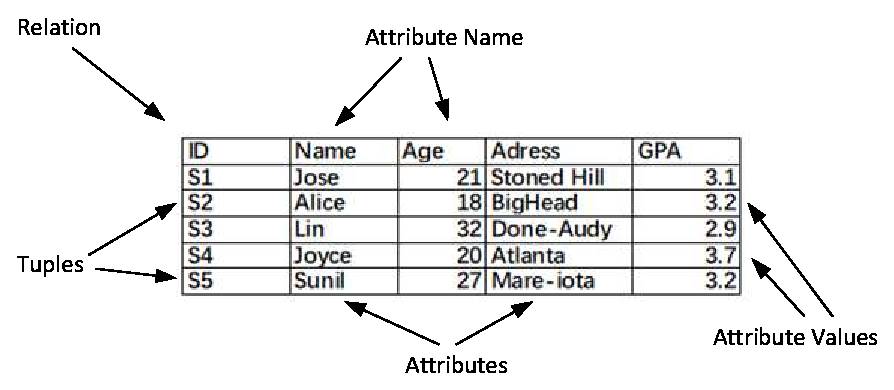
\includegraphics[width=0.8\linewidth]{handout/img/1-relation.eps}
    \caption{关系模型}\label{fig:1-relation}
\end{figure}

关系模型的单目算子包括：
\begin{itemize}
    \item $\pi$投影Projection：从关系中选择出某些属性，形成新的关系。
    \item $\sigma$选择Selection：从关系中选择出满足某些条件的元组，形成新的关系。
    \item $\tau$排序Sort：根据某个属性对关系中的元组进行排序，形成新的关系。
    \item $\delta$去重Distinct：从关系中删除重复的元组，形成新的关系。
    \item $\gamma$分组Group：根据某个属性对关系中的元组进行分组，形成新的关系。
\end{itemize}

\begin{figure}[H]
    \centering
    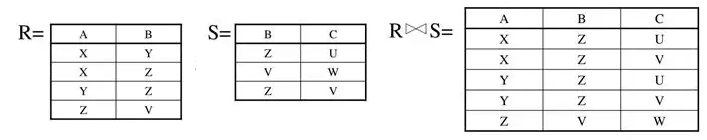
\includegraphics[width=\linewidth]{handout/img/1-join.png}
    \caption{自然连接双目算子示意图}\label{fig:1-join}
\end{figure}

双目算子包括：
\begin{itemize}
    \item $\times$笛卡尔积Cartesian Product：将两个关系的所有可能组合形成新的关系。
    \item $\bowtie$自然连接Natural Join：根据两个关系中公共属性的值进行连接，形成新的关系。
    \item $\bowtie_{c}$ $\theta$连接：根据两个关系中某个属性的值进行连接，形成新的关系。
    \item $\cup$并Union：将两个关系合并成一个新的关系，去除重复的元组。
    \item $\cap$交Intersection：从两个关系中选择出同时满足两个条件的元组，形成新的关系。
    \item $-$差Difference：从第一个关系中删除出同时出现在第二个关系中的元组，形成新的关系。
\end{itemize}

关系模型的更多内容，可以参考数据库原理课程的教材\cite{Ullman1998A}，这里仅简单回顾。

关系模型本质上是一种封闭的代数系统，其基本元素是关系Relation，关系间的运算仍然在这个代数系统上封闭。注意，虽然在实现上，关系是row的集合，但在关系运算中，Relation是基本单位而不是更小的tuple。

\begin{exercise}
    数学上，什么是系统？能举出某个学科上类似的例子吗？
\end{exercise}
\begin{exercise}
    Relation定义了单目、双目操作，这些操作够吗？一个复杂的查询总是能够通过这些操作的组合完成？
\end{exercise}
\begin{exercise}
    单目操作、双目操作，有没有三目操作？更多目操作？
\end{exercise}

\subsection{关系表达式}

一个关系$R$，经过单目操作选择后得到一个新的关系$\sigma_c(R)$，两个关系$R,S$，经过一个双目操作，得到一个新的关系$R\bowtie S$。这些算子组合起来，就可以形成一个复杂的查询表达式。例如，$R,S$关系分别先经过选择和投影，然后再连接：
$$\sigma(R) \bowtie \pi(S)$$
这些表达式称为关系表达式。关系表达式可以通过树形结构表示，如\figurename\ref{fig:1-relation-tree}所示。

\begin{figure}[H]
    \centering
    \begin{tikzpicture}[
        level distance=1cm,
        level 1/.style={sibling distance=2cm},
        level 2/.style={sibling distance=1cm},
        every node/.style={
            align=center,
            font=\small
        },
        edge from parent/.style={
            draw,
            -,
            shorten >=2pt,
            shorten <=2pt
        }
    ]
    % 根节点 - 连接操作
    \node {$\bowtie$}
        child {
            % 左子树 - 选择操作
            node {$\sigma$}
            child {
                % 叶子节点 - 关系R
                node {$R$}
            }
        }
        child {
            % 右子树 - 投影操作
            node {$\pi$}
            child {
                % 叶子节点 - 关系S
                node {$S$}
            }
        };
    \end{tikzpicture}
    \caption{关系表达式 $\sigma(R) \bowtie \pi(S)$ 的树型结构}\label{fig:1-relation-tree}
\end{figure}

关系表达式与树型结构是一一对应的，树的每个节点表示一个操作，叶子节点表示基本关系。通过这种树形结构，可以清晰地表示复杂的关系运算过程。后文在讲述查询处理时，对关系表达式和这种树型表示不加区分，二者是同一的。

在数据库原理课程里\cite{Ullman1998A}，还会介绍SQL语言，SQL语言是关系模型的一种查询语言，通过SQL语句可以方便地对关系数据库进行查询、更新、删除等操作。仅就SQL的查询功能而言，一条语句最终会对应于一个关系表达式。换句话说，SQL语言的设计目标就是能够方便地表达关系表达式。

与C语言不同，C语言是一种命令式语言，它最终的目标是将高级语言翻译成CPU上的指令序列，它的模型是一个栈指令机。SQL语言则要将查询语句翻译成关系表达式，然后选择算子的实现算法，最终生成高效的查询计划。SQL语言的设计与通用语言相比要简单得多，但要记住，它的目标是翻译成关系表达式，而不是CPU指令。

\begin{exercise}
    定义在整数集合上的加减运算，构成了一个代数系统，并由此衍生出代数表达式。代数表达式可以有许多等价表达，例如$a+(b+c)=(a+b)+c$。等价表达式有几多？类似的，关系表达式的等价表达式呢？——这暗示着什么？查询方案可以有$n$多。接下来的问题是，在特定系统中，是否存在一个最简的等价表达式，使得查询代价最低？寻找这样的最简表达式是否可行？
\end{exercise}
\begin{exercise}
    SQL查询语句得到的是什么？关系还是元组？有没有可能得到一个标量？
\end{exercise}

\section{关系数据库结构}

经过多年的发展，关系数据库的内部结构相对稳定下来，如\figurename\ref{fig:1-arch}所示。数据库内部主要有三个核心部件：执行引擎、存储引擎、事务引擎，除此外，还包含与客户对接的会话层接口等。

\begin{figure}[H]
    \centering
    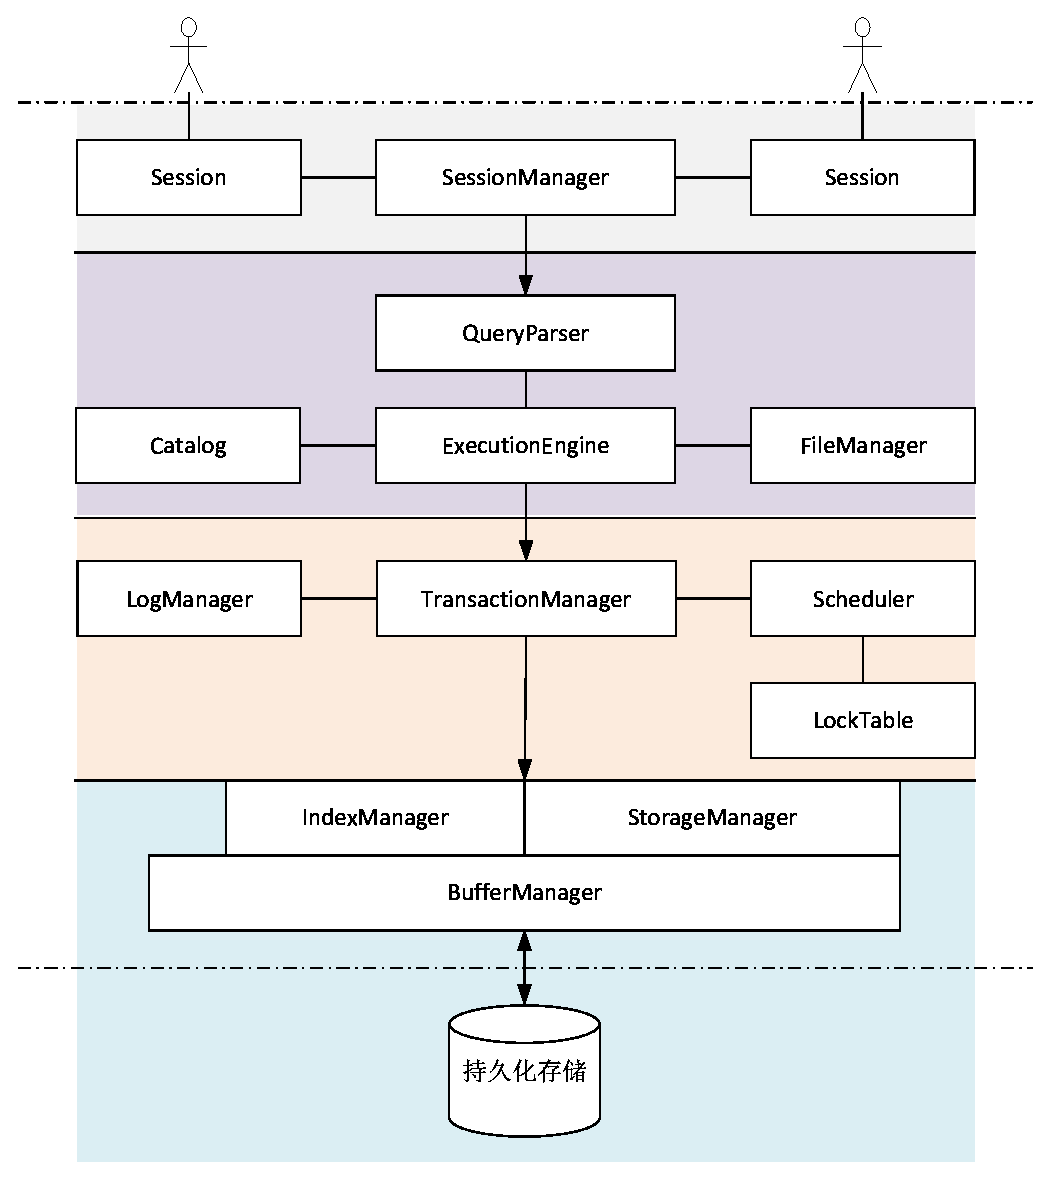
\includegraphics[width=\linewidth]{handout/img/1-arch.eps}
    \caption{关系数据库的内部结构}\label{fig:1-arch}
\end{figure}

\subsection{会话层}

一般情况下，关系数据库会部署在一个服务器上，客户端通过网络连接到数据库服务器，发送各种SQL语句。会话层负责处理客户端的连接请求，管理用户会话状态，并将SQL语句传递给执行引擎，在用户看来，会话层就是用户的代理。

有些嵌入数据库，例如SQLite，会直接将SQL语句传递给执行引擎，而不需要会话层，因为整个数据库运行在用户进程内。会话层为连续用户而设置，看成client/server模型，这里自然会有并发的问题。要保证并发的安全，要引入事务概念，这由事务引擎处理。会话层面临的问题是，如何高效地管理多个用户的连接，如何处理用户的认证和权限管理等。

完整数据库系统一般会以线程/进程形式支持多个用户的并发连接。每个用户连接会对应一个会话，会话层会负责管理这个会话的状态，包括认证、权限检查、查询处理等。随着互联网的发展，对数据库的一个挑战是如何支持大规模的并发连接。线程/进程模型在单机上支持的并发连接数量有限，未来可能会以协程方式提供会话服务。

会话层上另一个值得关注的问题是，会话代理用户执行SQL语句，它是SQL语句执行的主体，前述的执行引擎、事务引擎、存储引擎都要看成库，是会话调用执行引擎执行SQL语句。一个事务开始，中间结果、当前状态都是依附会话而存在，都要看成会话的局部变量。

\begin{exercise}
    会话接受用户SQL指令执行，将指令集看成指令流。指令流的执行是分节的，每个事务是一个小节。根据这个特性设计一个内存管理器arena，用于管理会话的局部变量。可以参考leveldb\cite{GitHubgo38:online}的arena方案。
\end{exercise}

\subsection{执行引擎}

会话收到用户的SQL语句，调用执行引擎的QueryCompiler将SQL语句编译成查询计划。这一过程包括语法分析、语义分析、逻辑优化、物理优化等阶段，最终生成一个查询计划。逻辑上，执行计划可以看成一个关系表达式的实例化，一个树型结构，叶子节点对应于关系，内部节点对应于某个关系算子，按照深度优先遍历方式执行。

以\figurename\ref{fig:1-relation-tree}为例，查询计划的执行过程如下：
\begin{enumerate}
    \item 从根节点开始，执行左子树，即选择操作$\sigma$，对关系R进行选择，得到关系R'。
    \item 然后执行右子树，即投影操作$\pi$，对关系S进行投影，得到关系S'。
    \item 最后执行连接操作$\bowtie$，将关系R'和关系S'进行连接，得到最终结果。
\end{enumerate}

在多数数据库实现中，你不会看到这种显式的树型结构执行计划，一般数据库都是用各种枚举器连接的算法。在\figurename\ref{fig:1-relation-tree}中，先调用$\sigma$算子实现函数，然后调用$\pi$算子实现函数，最后调用$\bowtie$算子实现函数。调用入口是$\bowtie$算子。——这称为火山模型volcano model。

\begin{figure}[H]
    \centering
    \begin{tikzpicture}[
        node distance=2cm,
        every node/.style={
            align=center,
            font=\small,
            minimum width=1.5cm,
            minimum height=0.8cm
        },
        operator/.style={
            rectangle,
            draw=blue!50,
            fill=blue!10,
            rounded corners=3pt,
            thick
        },
        data/.style={
            rectangle,
            draw=green!50,
            fill=green!10,
            rounded corners=3pt,
            thick
        },
        arrow/.style={
            ->,
            >=stealth,
            thick
        },
        callarrow/.style={
            ->,
            >=stealth,
            thick,
            blue,
            dashed
        },
        returnarrow/.style={
            ->,
            >=stealth,
            thick,
            red,
            dashed
        }
    ]

    % 火山模型 - 操作符调用层次
    \node[operator] (join) at (0,0) {$\bowtie$};
    \node[operator] (select) [below left=1.5cm and 1.5cm of join] {$\sigma$};
    \node[operator] (project) [below right=1.5cm and 1.5cm of join] {$\pi$};
    \node[data] (R) [below=1.5cm of select] {$R$};
    \node[data] (S) [below=1.5cm of project] {$S$};

    % 数据流箭头（实线）
    \draw[arrow] (R) -- (select);
    \draw[arrow] (S) -- (project);
    \draw[arrow] (select) -- (join);
    \draw[arrow] (project) -- (join);

    % 调用箭头（蓝色虚线）- 火山模型的核心
    \draw[callarrow] (join) to[out=180,in=90] (select);
    \draw[callarrow] (join) to[out=0,in=90] (project);
    \draw[callarrow] (select) to[out=180,in=180] (R);
    \draw[callarrow] (project) to[out=0,in=0] (S);

    % 添加标签说明
    % \node[anchor=west] at (-7,0) {\textbf{火山模型执行流程:}};
    \node[anchor=west] at (-7,0) {\textcolor{blue}{蓝色虚线}: 操作符调用};
    \node[anchor=west] at (-7,-0.5) {黑色实线: 数据流};

    \end{tikzpicture}
    \caption{火山模型（Volcano Model）执行流程}\label{fig:1-volcano-model}
\end{figure}

火山模型的执行过程可以描述为：
\begin{enumerate}
    \item 根操作符$\bowtie$开始执行，调用其子操作符$\sigma$和$\pi$
    \item 每个子操作符递归调用其子操作符（叶子节点直接访问数据）
    \item 数据从叶子节点逐级向上返回
    \item 每个操作符处理接收到的数据，生成新的数据
    \item 最终结果从根操作符输出
\end{enumerate}

这种模型之所以称为火山，是因为数据从底层向上喷发，经过各个操作符的处理，最终从顶部输出结果。火山模型的一个重要特点是每个操作符都实现了统一的接口，如open、next、close等。对于流式处理，火山模型可以使得某个tuple连续经过多个算子的处理，一次性输出结果，减少中间结果的存储开销，提高查询效率。火山模型的问题是，对指令缓存不友好，因为每个操作符调用都是函数调用，会导致频繁的上下文切换，影响CPU指令缓存的命中率。

\begin{exercise}
    构思一种方案，改善火山模型的指令缓存不友好问题。
\end{exercise}

QueryCompiler如何将SQL语句翻译成查询计划？SQL语言比较小巧，它的目标是最终将SQL语句翻译成关系表达式，然后选择具体的算子实现算法，最终生成查询计划。SQL语言的设计与通用语言相比要简单得多，但要记住，它的目标是翻译成关系表达式，而不是CPU指令。

\subsection{存储引擎}

关系数据库的存储引擎主要包含三个方面的功能：底层存储组织、索引结构、以及buffer缓冲。底层存储组织负责将关系数据存储在磁盘上，通常采用页page的方式进行存储，每个页包含多个记录record。索引结构用于加速数据的查询，多数数据库采用btree作为索引结构。buffer缓冲用于缓存最近访问的数据页，减少磁盘I/O操作，提高查询性能。

在\figurename\ref{fig:1-arch}中，会话执行SQL语句的执行计划，按照火山模型调用next迭代接口，访问某个关系$R$的元组tuple。返回tuple的过程有点长，存储引擎根据$R$名到数据库元信息catalog中找到存储的文件名，打开文件，这里有文件管理的问题。文件打开，对应于一个文件描述符fd。这里我们还不了解btree索引结构，将它想象成一个$f(x)$函数，输入tuple的主键key，输出tuple在文件中的偏移量offset。拿到这个offset后，到缓冲管理器里根据$fd:offset$查找page，如果page不在缓冲区，就从磁盘加载page到缓冲区。页面调入缓冲后，在page内部找到tuple对应的记录，解析后返回给执行引擎。

\begin{figure}[H]
    \centering
    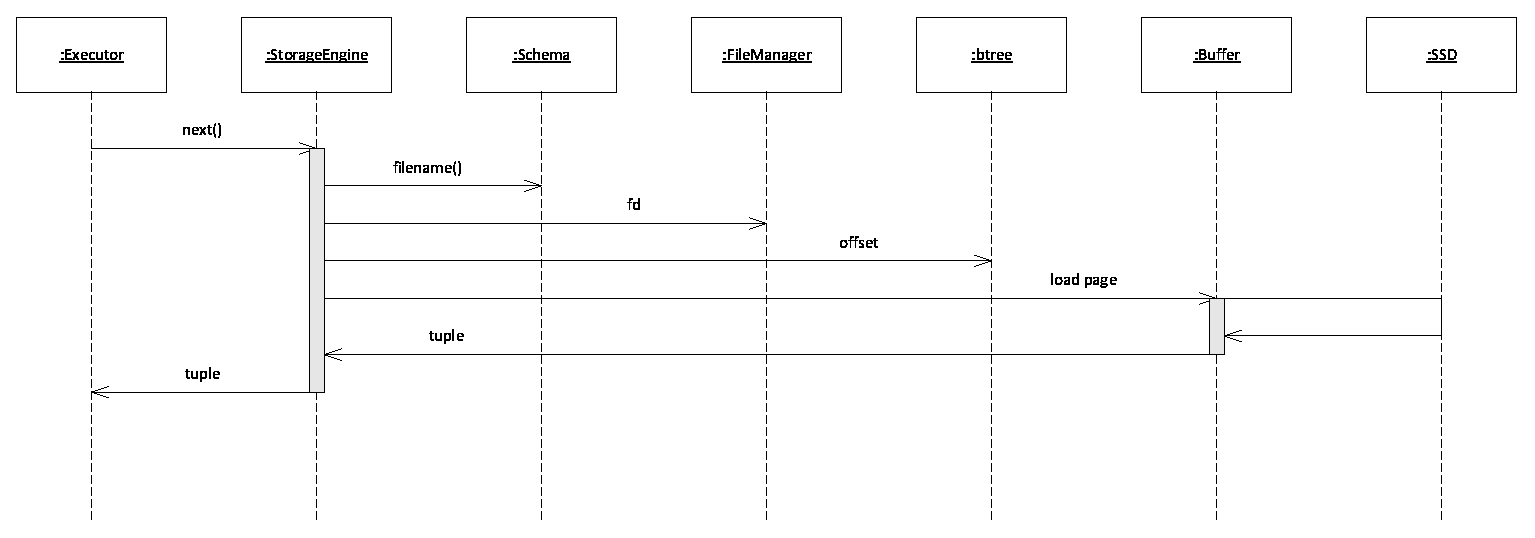
\includegraphics[width=1.2\linewidth]{handout/img/1-tuple.eps}
    \caption{存储引擎返回tuple过程}\label{fig:1-tuple}
\end{figure}

\begin{exercise}
    假设会话层用协程实现，协程模型为$m:n$，有$n$个线程，有远多于$m>>n$的协程，当协程等待异步结果，协程被挂起。编写open\_page()函数伪码，从HDD/SSD上读出page到缓冲区。
\end{exercise}

\subsection{事务引擎}

事务是数据库领域的一个抽象概念，一个事务看成是一组执行流，将数据库的数据看成公共的资源，事务对公共资源的访问要遵循一定的规则，否则会导致不一致问题，例如某个事务正在修改某个银行账户上的余额，另一个事务正在读取这个余额，如果不加控制，就会导致读取到不一致的数据。

事务的概念其实并不仅限于数据库系统，以一个web服务为例，它后台挂着一个数据库，通过web服务暴露API给用户使用。用户连接数据库后，发起一个事务，从物理边界上看，事务涵盖着用户端、web服务端、数据库端多个部分，要将这些部分看成一个整体，才能理解事务的意义。

事务具有原子性、一致性、隔离性、持久性（ACID）等特性。原子性指事务要么全部成功，要么全部失败；一致性指事务执行前后，数据库要保持一致的状态；隔离性指多个事务并发执行时，要相互隔离，避免互相干扰；持久性指事务一旦提交，其结果要永久保存。

ACID原则中，最难理解的是一致性，何谓一致的状态？一致性其实是用户的约束，不同的系统有不同的约束。站在数据库的角度，如何保证一致性？数据库的数据访问抽象为read/write两种操作，数据库的一致性要保证多个事务并发执行时，read/write是一致的。

\begin{exercise}
    事务的原子性要求事务执行得非常快？与CPU的原子指令有何区别？
\end{exercise}

事务引擎主要处理两方面的工作：事务并发、故障恢复。并发目前常用的方案是：基于锁的并发控制、基于时间戳的并发控制。故障恢复则主要通过日志记录和检查点机制实现。

在\figurename\ref{fig:1-arch}中，事务引擎的主要工作是控制会话的执行流。在实现中，事务代码一般是嵌入到执行引擎、存储引擎代码中，控制事务的开始、提交、回滚等操作。以\figurename\ref{fig:1-relation-tree}为例，当读取关系$R$，会对$R$的每个tuple加锁，防止其他事务修改$R$。当读取关系$S$，会对$S$的每个tuple加锁，防止其他事务修改$S$。当事务提交时，会释放所有加的锁。

 % 1
\chapter{Layout}\label{chap:layout}

本章介绍数据库中常见的存储布局layout，包括关系数据库、kv数据库的存储布局。

\section{存储介质}

在组成原理的课程中，计算机体系结构中的存储介质呈现金字塔结构，从上到下分别是：寄存器、缓存、主存、硬盘等，如\figurename\ref{fig:2-pyramid}所示。数据是数据库最重要的资产，数据是保存在持久化介质中。

\begin{figure}[H]
    \centering
    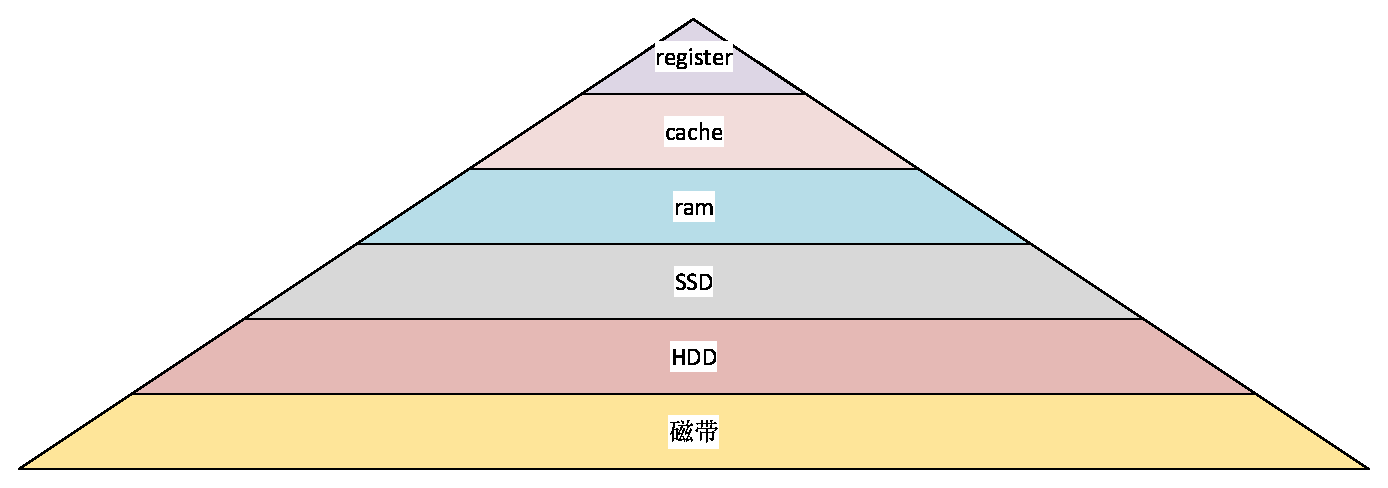
\includegraphics[width=\linewidth]{handout/img/2-pyramid.eps}
    \caption{存储介质金字塔结构}\label{fig:2-pyramid}
\end{figure}

\subsection{HDD}

传统的HDD硬盘，采用机械结构定位磁头，磁头以磁臂的轴心滑动，磁盘高速旋转在磁头感应出微弱信号，信号经过放大，转换为电信号，磁盘控制器通过DMA传送到内存，由CPU接手操作。

\begin{figure}[H]
    \centering
    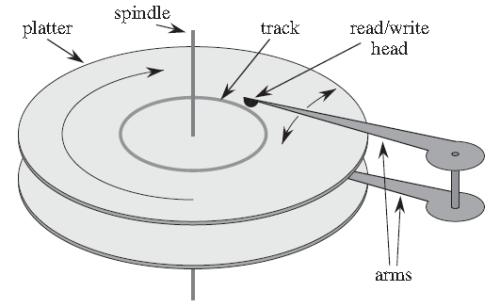
\includegraphics[width=0.5\linewidth]{handout/img/2-hdd.png}
    \caption{HDD硬盘机械结构}\label{fig:2-hdd}
\end{figure}

HDD盘片的双面喷涂磁性材料，这样就需在盘片上下布局磁头。同时，为了增加磁盘容量，会串接多个盘片。每个盘的表面，都有多个磁道，每个磁道上有多个扇区，如\figurename\ref{fig:2-sector}所示。多个磁头的磁臂被固定在一起，当磁臂滑动，所有磁头都滑动到相同位置上。这样，多个盘片的同心磁道组成了一个柱面cylinder。

磁盘的传输单位是扇区sector，通常每个扇区512B。传统HDD硬盘，为定位一个扇区，采用柱面-磁头-扇区3D(Cylinder-Head-Sector)方式定位。这种3D定位方式与厂商的实现有关，不同厂商可能采用不同的方式。为了简化BIOS实现，现代HDD硬盘，通常采用LBA(Logical Block Address)方式定位扇区。LBA方式将柱面-磁头-扇区3D定位方式，映射为一个线性地址，这样就可以用一个简单的整数来定位一个扇区。

\begin{figure}[H]
    \centering
    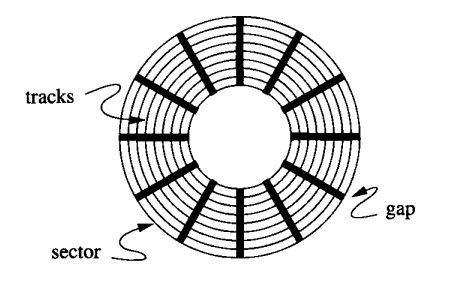
\includegraphics[width=0.6\linewidth]{handout/img/2-sector.png}
    \caption{HDD扇区}\label{fig:2-sector}
\end{figure}

由于HDD硬盘读写采用机械结构定位磁头，寻道时间比较长，一般在10ms左右，旋转延迟一般在5ms左右。传输延迟是将数据从磁盘传送到内存的时间，由于是电信号，延迟很小。

为了加速HDD访问，一般有几种方案：设置缓冲，电梯算法，临近存放，RAID并行等。

\begin{exercise}
    证明磁头的平均移动距离是总距离的1/3。
\end{exercise}
\begin{exercise}
    一般文件系统以block为单位提供存储服务，每个block包括多个扇区，通常为4KB。文件系统声称一个操作是原子的，是指这个操作很快吗？如果不是，那是指的什么？
\end{exercise}
\begin{exercise}
    journal文件系统是一种日志文件系统，它将所有修改操作记录在日志文件中，然后再进行实际的修改。这样可以避免在修改过程中发生故障，导致数据丢失。它是如何实现原子操作的？
\end{exercise}

\subsubsection*{临近存放}

假设一个文件比较大，文件会包含多个扇区。一般文件系统管理磁盘的时候，随着文件增大，按需分配扇区。如果不采取措施，这个文件的扇区会随机分别在磁盘上，IO开销会很大。并且，随着系统运行时间增加，通常而言，磁盘上的文件组织呈现碎片化，有些文件系统会在后台尝试整理硬盘，挤压碎片。

临近存放的策略是，每次文件增长时，申请足够多的扇区数目，文件系统一般会顺序在磁盘上分配，这些分配的扇区会以很高的概率分配在临近的柱面上。如前所述，所有磁头是同步固定的，这样一来就节省了寻道时间。

\begin{exercise}
    Google的文件系统GFS，它每次分配文件都按照一个chunk为单位，每个chunk默认是64MB。解释一下，这种策略的优势。
\end{exercise}

\subsubsection*{RAID}

RAID(Redundant Arrays of Independent Disks)冗余磁盘阵列将多个物理磁盘组合成一个逻辑磁盘，提供数据冗余和性能提升。标准规定了RAID 0-5，RAID 6由厂商自定义。

\begin{exercise}
    查找资料，学习RAID 0-5，RAID 6的原理，包括条带化、镜像、校验、均衡等手法。
\end{exercise}

HDD受限于机械结构，IO访问时间一般平均在10ms左右，相比于CPU执行执行，非常慢。现代CPU执行一条指令平均在2ns左右，两者相比，HDD的IO访问时间是CPU执行指令的100,000-1,000,000倍。所以，在数据库领域，衡量数据库性能，一般计算对HDD硬盘的访问次数就够了。

\begin{figure}[H]
    \centering
    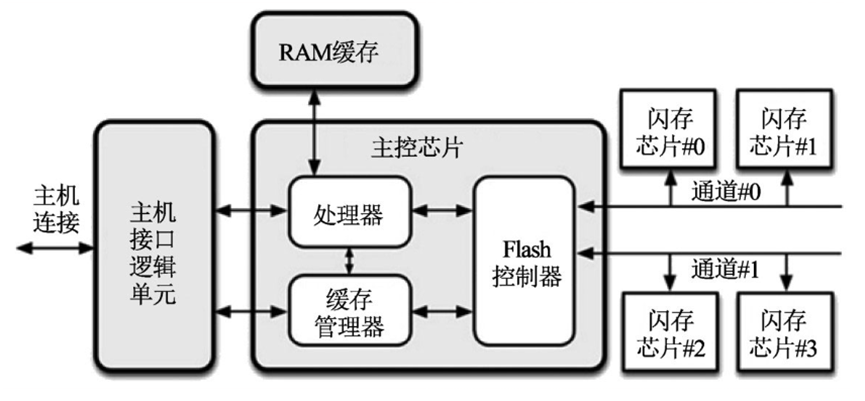
\includegraphics[width=0.8\linewidth]{handout/img/2-ssd.png}
    \caption{SSD内部结构}\label{fig:2-ssd}
\end{figure}

\subsection{SSD}

随着SSD硬盘的普及，目前大量数据库系统采用SSD硬盘作为存储设备。SSD设备没有机械结构，使用支持NVMe协议的M.2接口的随机读写速度一般都在1000KIOPS之上，延迟一般在250us左右。相比于CPU指令执行，SSD的IO访问时间是CPU执行指令的50,000-100,000倍左右。

SSD内部基本上是一个mini的计算机系统，从PCIe通道发送来的速写指令传递到SSD，SSD内部会解析指令，根据指令进行数据读写。SSD内部有多个NAND flash内存芯片，每个芯片有多个页page，每个页有多个块block，每个块有多个扇区sector。SSD内部有一个控制器，负责接收指令，解析指令，根据指令进行数据读写。

SSD的NAND flash器件，与硬盘的读写特性不一样，它有三种操作：读、写和擦除。读写操作是将数据从内存写入NAND flash，或者从NAND flash读取数据到内存。擦除操作是将NAND flash上的一个块全部擦除，变成未写状态。三种操作的耗时是不同，读最快，写大约比读慢10倍，擦除大约比读慢100倍。

\begin{table}[H]
    \centering
    \caption{HDD与SSD性能对比}
    \label{tab:2-hdd-ssd-comparison}
    \begin{tabularx}{\linewidth}{lXXX}
        \toprule
        \textbf{指标} & \textbf{HDD（机械硬盘）} & \textbf{SSD（固态硬盘）} & \textbf{倍数（近似）} \\
        \midrule
        顺序读取带宽 &
        \begin{minipage}[t]{\linewidth}
            100～200MB/s
        \end{minipage} &
        \begin{minipage}[t]{\linewidth}
            7,000MB/s
        \end{minipage} &
        \begin{minipage}[t]{\linewidth}
            70倍
        \end{minipage} \\

        随机读取 IOPS &
        \begin{minipage}[t]{\linewidth}
            50～150 IOPS
        \end{minipage} &
        \begin{minipage}[t]{\linewidth}
            10,000～1,000,000+ IOPS
        \end{minipage} &
        \begin{minipage}[t]{\linewidth}
            100～10,000 倍
        \end{minipage} \\

        访问延迟 &
        \begin{minipage}[t]{\linewidth}
            5～15 毫秒（ms）
        \end{minipage} &
        \begin{minipage}[t]{\linewidth}
            0.01～0.1 毫秒（即 10～100 微秒）
        \end{minipage} &
        \begin{minipage}[t]{\linewidth}
            约 50～1,000 倍
        \end{minipage} \\
        \bottomrule
    \end{tabularx}
\end{table}

SSD盘为了兼容HDD的文件接口，会在SSD内部实现Garbage Collection机制，对block的修改会先写入到一个空闲的block中，然后将原来的block标记为已删除。当SSD内部的block被写满后，会触发垃圾回收，将已删除的block中的数据复制到新的block中，释放空间。

SSD的GC与文件系统在功能上存在语义重叠，二者工作在不同层次、缺乏协同，因信息不对称导致效率损失。例如，文件系统的空闲对SSD是不可见的：
\begin{enumerate}
    \item 用户删除一个1GB文件 $\rightarrow$ 文件系统在元数据上标记 LBA [1000–2000] 为空闲。
    \item SSD并未收到回收这些LBA的通知，仍然认为这些LBA的物理页是有效数据，因此不会被回收。
\end{enumerate}
现代系统引入跨层通信协议，文件系统在删除文件后，向 SSD 发送 TRIM 命令，告知：“LBA X–Y 已不再使用”。SSD 的 FTL 将这些 LBA 对应的物理页标记为“无效”。更新的方案是将SSD的GC机制与文件系统的空闲管理机制进行整合，将SSD的部分功能上移到文件系统，使其能够直接管理物理块。

\begin{exercise}
    查找ZNS SSD / Open-Channel SSD资料，了解跨层文件系统整合方案。
\end{exercise}
\begin{exercise}
    在HDD上，采用预分配大块连续LBA的方案，利用临近柱面寻道事件短的优势，提高IO性能。查找SSD的相关资料，基于SSD并行访问的物理构架，能否提出一种LBA预分配方案，提升IO读写性能。
\end{exercise}

\section{数据库文件}

数据库管理系统一般包括数据文件、索引文件、日志文件、元数据文件、配置文件等。这些文件的通途不同，访问模式也不同。数据文件用于存储tuple数据，关系型数据库的数据文件通常是分页的，索引文件的结构一般与数据文件类似。日志文件用于记录数据库的操作，以便在系统故障时进行恢复，它的操作一般是追加。元数据文件用于存储数据库的结构信息，例如表、索引、约束等，很少修改。配置文件用于存储数据库的配置参数，例如缓存大小、IO 调度策略等，更少修改。

\begin{figure}[H]
    \centering
    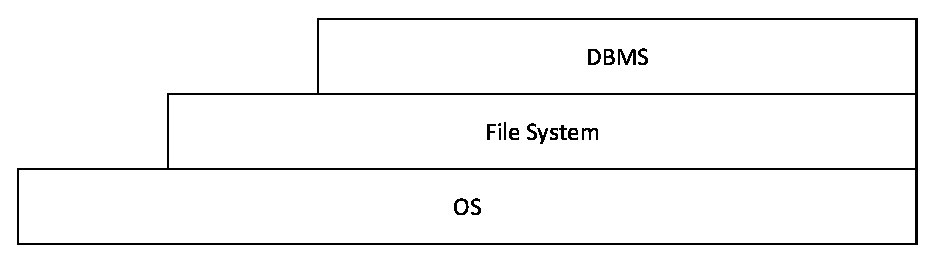
\includegraphics[width=0.8\linewidth]{handout/img/2-dbms.eps}
    \caption{数据库与文件系统}\label{fig:2-dbms}
\end{figure}

大多数数据库管理系统会以文件作为存储单位，将数据文件、索引文件、日志文件、元数据文件、配置文件等存储在不同的文件中，如\figurename\ref{fig:2-dbms}所示。极少数软硬件通吃的厂商会将DBMS直接集成在操作系统中，让DMBS直接管理HDD/SSD等存储设备。

\begin{figure}[H]
    \centering
    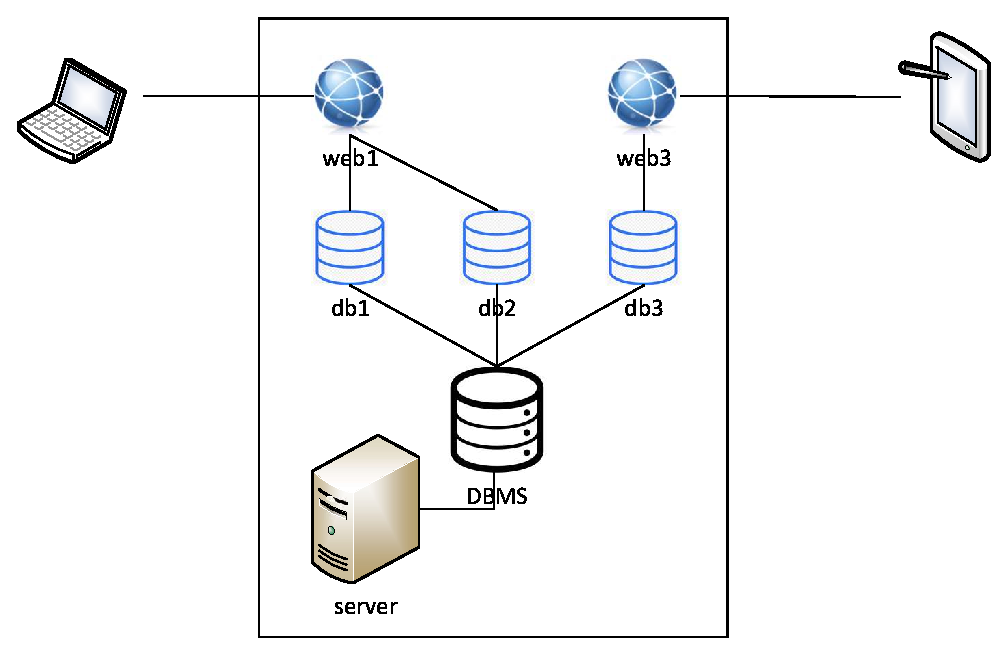
\includegraphics[width=0.9\linewidth]{handout/img/2-deploy.eps}
    \caption{数据库部署}\label{fig:2-deploy}
\end{figure}

在DBMS中，一般假设，一个关系对应于一个数据或多个数据文件，很少会将一个数据文件用于存储多个关系。最简单的方案是每表一文件，即规定每个关系对应于一个数据文件。但复杂构架下的数据库，数据文件可能跨节点分布式存储，一个关系可能对应于多个文件。

DBMS部署一般的模型如\figurename\ref{fig:2-deploy}所示，一个DBMS实例对应于一个物理节点，一个DBMS实例可以运行多个数据库实例。Oracle比较特别，它不支持CREATE DATABASE，每个用户拥有自己的Schema，而不是数据库实例。

考虑到存储的异质，HDD/SSD它们的特性完全不同，PostgreSQL引入表空间概念，用一个目录表示特定存储设备，表的数据文件可以存在不同的表空间中，一个表空间也可以容纳多个表的数据文件。Innodb/Oracle则不同，它们的表空间概念是逻辑上的，一张表对应于一个表空间，表空间容纳多个该表的数据文件。

\subsection{分页}

考虑一个Relation如何将它的tuple存放在一个文件中。最简单的模型，将文件看成一个连续堆，tuple直接顺序写入文件。这种模型简单直接，但是tuple可能会修改删除，从而导致文件碎片化，降低IO性能。

\begin{figure}[H]
    \centering
    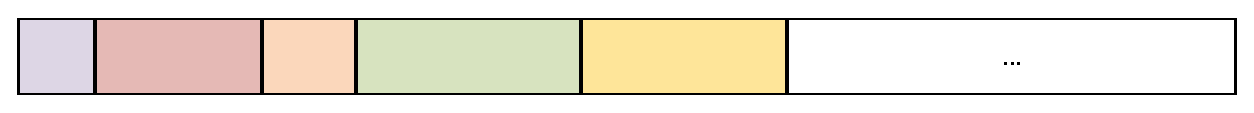
\includegraphics[width=0.8\linewidth]{handout/img/2-heap.eps}
    \caption{简单的堆模型}\label{fig:2-heap}
\end{figure}

操作系统的内存管理可以分段、分页，将物理内存分成固定大小的页，小内存从页面上分配，碎片化仅在页内，不会影响整体性能。借鉴这种思路，数据库的文件管理也可以采用分页的方式，将文件分成固定大小的页，tuple存放在页内。

\begin{figure}[H]
    \centering
    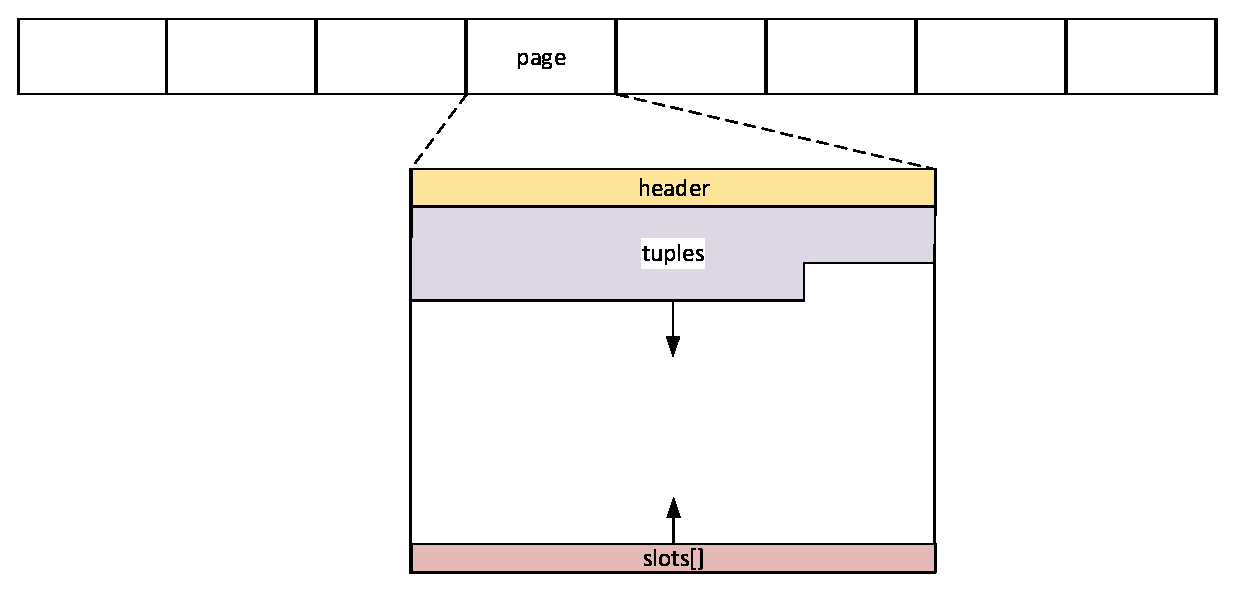
\includegraphics[width=\linewidth]{handout/img/2-page.eps}
    \caption{数据文件分页模型}\label{fig:2-page}
\end{figure}

按照\figurename\ref{fig:2-page}所示，数据文件按照page大小分页存储，每个页包含多个tuple。为管理页面内部的tuple，页面有特定格式，前部是固定大小的头部header，然后是tuple载荷，页面的后部是slots[]数组。slots[]数组用于记录每个tuple的偏移量和大小，方便数据库管理系统快速定位和访问tuple。tuples和slots大小可变，因此分别位于空闲区域的上下两侧，从两个方向扩展。

数据文件分页后，数据库可以管理自己的缓冲，由于页面大小固定，数据库的缓冲设计相对简单。相对于OS缓冲，数据库更了解这些页面的用途，哪些页面可以直接drop掉，哪些页面需要回写。而OS内核缓冲由于难以获取这些信息，缓冲效率较低。

\begin{exercise}
    操作系统一般配置了虚拟内存，当物理内存不敷使用时，会将一部分内存分页转储到硬盘上，称为交换空间。分析一下，当数据库系统进程切换时，数据库的页面是否会被放到交换空间中？如果会，会有什么影响？
\end{exercise}
\begin{exercise}
    数据库日志文件一般会以O\_APPEND模式打开，即每次写入日志时，会将数据追加到文件末尾，而不是覆盖原有内容。Linux系统将这种写入称为原子的，追加写入是否安全？有何风险？
\end{exercise}
\begin{exercise}
    Innodb的数据文件每次扩容，按照extend机制增长，extend最初为8MB，后续会动态增加到64MB。Innodb为什么会引入extend机制？
\end{exercise}

\subsection{分段}

数据文件分页，其设计目标主要是为了容纳tuple，减少碎片化，提升性能。除了容纳tuple外，数据文件其实还有更多的需求，如垃圾收集、容纳BLOB等、维持多版本、构建索引等。

在数据文件内部分段，是基于功能的考虑：存储tuple的数据段、构建索引的索引段、容纳BLOB的溢出段、维持旧版本的堆段。数据文件内的页面根据功能和用途，被划分的不同的逻辑段。

\subsubsection*{超块}

数据文件的头部一般存储该数据文件的一些元信息，包括文件大小、空闲链表指针等，本文称为超块superblock。超块的目的是为了描述该数据文件，给出数据文件内部各段的起始位置和大小等信息。

\begin{figure}[H]
    \centering
    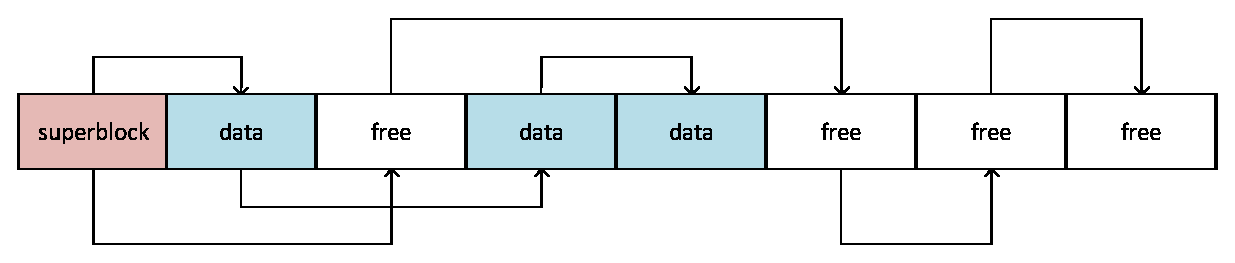
\includegraphics[width=\linewidth]{handout/img/2-superblock.eps}
    \caption{超块页面}\label{fig:2-superblock}
\end{figure}

\begin{exercise}
    超块用于描述数据文件，为了防止对超块的写入错误，超块该如何设计？采用日志，描述超块的修改操作？或者使用双超块？
\end{exercise}

\subsubsection*{垃圾收集与空闲链表}

btree在合并页面后，会废弃一些旧的页面，这些页面被称为空闲页面，空闲页面会被加入到空闲链表中。数据文件在增长时，也会出现空闲页面，这些页面会被加入到空闲链表中。空闲页面以单向链表的形式组织，每个页面包含一个指向下一个空闲页面的指针，如\figurename\ref{fig:2-superblock}。

\begin{exercise}
    为什么不采用双向链表组织空闲页面？或者其它结构？
\end{exercise}

\begin{exercise}
    数据文件如果部署在SSD，该如何管理空闲页面？采用前述的空闲链表，显然有问题。写入后继指针意味着该页面脏，当重新启用该空闲页面，SSD控制器需要从内部的干净页面上再分配来替换这个空闲页面。该用什么方案来解决这个问题？
\end{exercise}

\subsubsection*{溢出页面}

当tuple对应的record尺寸超过页面大小，会发生溢出。溢出部分需要存放在其余页面中，这些页面称为溢出页面。异常页面的头部仍然是固定大小的，与普通数据页面格式相同，只是slots数组可以不再需要。溢出页面需要专门的段来容纳？不需要，它是普通页面的附属。

\begin{figure}[H]
    \centering
    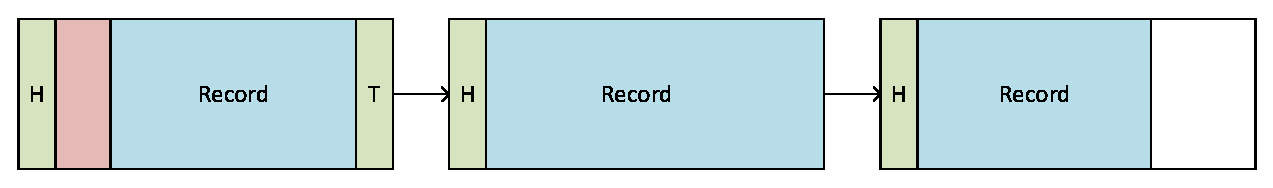
\includegraphics[width=\linewidth]{handout/img/2-blob.eps}
    \caption{溢出页面}\label{fig:2-blob}
\end{figure}

\subsubsection*{旧版本/undo页面}

在MVCC并发控制的数据库系统中，如PostgreSQL/Oracle等，每个key对应于多个版本，版本之间通过时间戳区分，以单向链表形式组织。有些MVCC系统，将旧版本存放在单独的旧版本页面中，而不是与当前版本页面混合在一起。原因是当前版本一定是访问最多的，旧本部访问概率较小，数据页面容纳的record会更多，有助于提升性能。

旧版本页面一般采用堆模型，不会再聚集，这是后面的聚集存储的知识，这里先提一句。旧版本页面一般采用单向链表组织，构成一个段。

\section{Record}

逻辑上，Relation由tuple构成，每个tuple包含多个字段，每个字段有特定的类型。在数据库层面，由于创建的表各不相同，每个关系的tuple字段数量和类型也不同。存储在页面上的tuple，有特定的格式，而不能是简单的字段序列。为区分逻辑上的tuple，将页面上存储的tuple称为记录record，记录带有一定的格式，根据这个格式能够区分出各个字段的长度。

\subsection{记录格式}

站在数据库的角度，记录中字段类型和长度是变化的，完全依赖于Schema不可行。例如，一个变长字符串VarChar(10)，它是说这个字段最长10B，字段长度是不定的，如果在记录中保留10B空间，会使得存储效率低下，IO效率也会降低。因此，记录需要有一定的自解释能力。

记录格式的设计基本要求是能够描述各字段的长度，各数据库的设计有很大不同，这里给出的设计参考了Innodb的方案，但与之稍有不同。如\figurename\ref{fig:2-record}所示，记录主要包含以下几个部分：

\begin{itemize}
    \item header，定长，包含记录的一些元信息，tomstone标记，溢出标记等。
    \item total，变长，记录完整长度。
    \item offsets，变长数组，记录中所有字段的偏移量，偏移量从offsets结尾开始计算，每个偏移量仍然是变长整数。
    \item fields，变长数组，记录中所有字段的实际数据，每个字段的长度根据offsets中描述的偏移量和下一个偏移量之间的差值确定。最后一个字段的长度，需要total参与计算。
    \item pads，填充为0，对齐8B。
\end{itemize}

\begin{figure}[H]
    \centering
    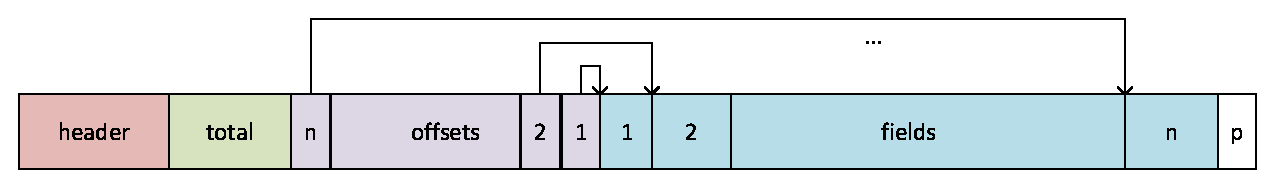
\includegraphics[width=\linewidth]{handout/img/2-record.eps}
    \caption{记录格式}\label{fig:2-record}
\end{figure}

整个记录的设计要点是，使用各字段的offset来计算字段的长度，offsets按照逆序排列，第1个字段的offset排在最后且为0。这样offsets数组虽然每项都是变长的，数目也不确定，但是数值是单调递减到0，从而能够识别出整个offsets数组，不需要Schema的参与。

Innodb中，记录中保存的是各字段的长度，虽然也是逆序保存，但并不象offset一样具有单调性，必须依赖Schema指示字段个数。

\begin{figure}[H]
    \centering
    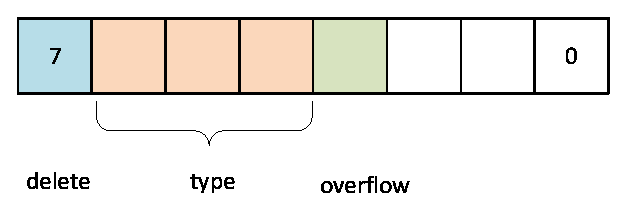
\includegraphics[width=0.5\linewidth]{handout/img/2-header.eps}
    \caption{记录头格式}\label{fig:2-header}
\end{figure}

记录的头部长度固定，暂定为1B，bit7表示tomestone标记，bit6-4是类型标记，bit3表示溢出标记，最低3bit保留。记录类型用于标记是何种类型，有些记录可以使用各种压缩方案。

\subsection{溢出记录}

溢出记录会跨页面保存，如\figurename\ref{fig:2-blob}所示。为响应溢出需求，在记录的header后部添加next字段，该字段定长，指向记录存储的下一个页面。如\figurename\ref{fig:2-overflow}，page2如果放不下，会继续分配页面容纳溢出记录，后续页面之间通过后继指针连接。next字段后是变长的first字段，它指明记录在该页面中的存放大小。next/first字段要尽可能排列在记录的前部，以避免从这两个字段被截断。

溢出记录在截断时，按照8B对齐，不填充。

\begin{figure}[H]
    \centering
    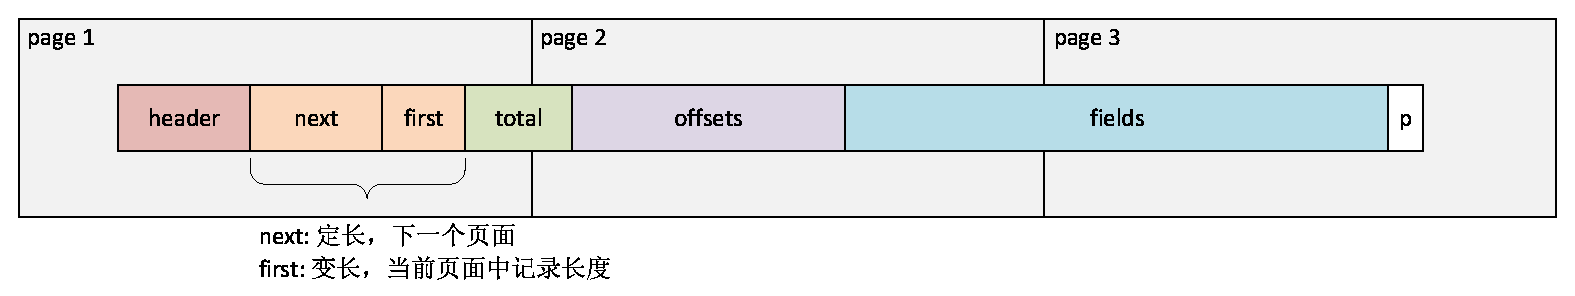
\includegraphics[width=\linewidth]{handout/img/2-overflow.eps}
    \caption{溢出记录跨页面保存}\label{fig:2-overflow}
\end{figure}

\subsection{xmin/xmax}

在PostgreSQL这样的堆存储方案中，由于支持MVCC，一般会在记录中添加xmin/xmax字段，用于记录该记录的可见性。xmin表示该记录被哪个事务创建，xmax表示该记录被哪个事务删除。如\figurename\ref{fig:2-mvcc}，根据key找到记录的位置，然后从page上的slots定位到record1，这是最初的版本。所有版本一般会临近存放，按照从旧到新顺序指向。

\begin{figure}[H]
    \centering
    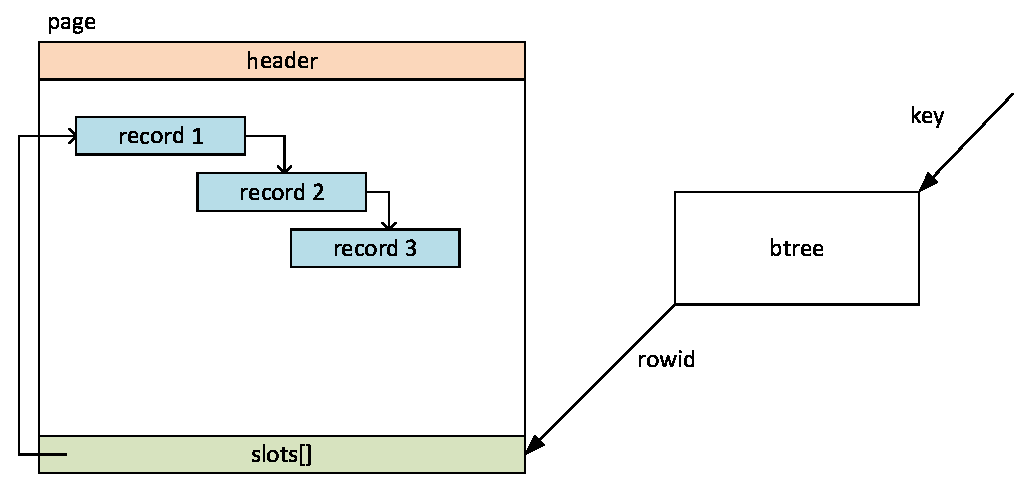
\includegraphics[width=\linewidth]{handout/img/2-mvcc.eps}
    \caption{PostgreSQL多版本存储}\label{fig:2-mvcc}
\end{figure}

在PostgreSQL的非聚集存储方案中，rowid并非是tuple的id，它是一个复合整型：利用某些位来表示页面号，利用其他位来表示的slots序号。拿到rowid后，会先找到对应的页面，然后再根据slots序号找到记录的offset，从而定位到记录。由于存在多个版本，为了快速定位到对应的版本，PostgreSQL的记录格式使用定长xmin/xmax，不需要打开记录格式，能够快速定位记录。

与PostgreSQL不同，Innodb是聚集存储，key临近的记录会聚集在临近的页面。但Innodb页面的slots需要按照key排序，这需要打开记录访问key。PostgreSQL中，btree指向的rowid一般是不动的。而innodb中，btree只需给出记录所在的页号，但页面插入一个记录后，该页面有可能分裂，导致btree指向的页号发生变化。——这是不同的设计选择带来的。

与PostgreSQL不同，Oracle的btree则指向最新的记录，新记录指向旧记录，与PostgreSQL刚好相反。旧记录并不就近保存，而是在旧版本段内维护。

\subsection{rowid}

rowid在堆存储模型中非常有用，它表示一条记录在数据库中的物理位置，用于快速定位一条记录，是一条记录的唯一标识符。rowid一般并不会暴露给用户，而是在系统内部使用。在聚集存储中，如innodb，一般直接使用key来定位记录，而不是rowid。

不同的数据库中，rowid的实现方式不同，甚至名字也不同。Oracle的rowid采用10字节存储，显示为18B的Base64字符串，格式如下：
\begin{lstlisting}[style=verbose]
OOOOOOFFFBBBBBBRRR
│     │   │     └─── Row number (3 chars) → 行在块中的位置（从 0 开始）
│     │   └───────── Block number (6 chars) → 数据块编号
│     └───────────── Relative file number (3 chars) → 相对文件号
└─────────────────── Data object number (6 chars) → 对象 ID
\end{lstlisting}

PostgreSQL的ctid与Oracle的rowid近似，它使用两个整型$[pageno, index]$表示一条记录：
\begin{itemize}
    \item pageno，int32，记录所在的页面编号。
    \item index，记录在页面中slots数组中的序号。
\end{itemize}

在实现中，rowid一般会采用变长表示，放在记录中，只有打开一条记录才能获取rowid。所以，不管是Oracle的rowid，还是PostgreSQL的ctid，不用担心rowid的长度问题。

在堆存储中，一般页面布局仍然采用\figurename\ref{fig:2-page}方式，只是页面尾部的slots数组不再是按照key排列，而是按照记录写入的先后顺序排列。这带来的问题是，如果删除一条记录，它的槽位会被保留，以免影响其它记录的定位。虽然损失的资源较小，后续可以安排一个扫描线程，回收这部分资源。

\section{kv存储}

传统关系型数据库主要使用btree作为索引，主要针对OLTP应用，这些应用一般要求读写平衡。21世纪以来，随着云计算、大数据的发展，大规模OLAP的应用需求逐渐占据主流地位，这些应用的特征是，采用批处理模型，批量写入而非更新，同时对读操作性能要求较高。在这种场景下，kv存储基于列存、无结构、IO效能较高，逐渐成为新型存储组织方式。

kv存储的需求主要来源于批处理场景，设想一下，源源不断的数据写入，如果使用传统的数据组织，还需要找到对应的位置插入，即使使用堆模型，也需将数据插入到结构化的页面中。最简单的方式是，将数据在内存里排好，当数据量超过一定阈值时，一把写入磁盘，也不用带什么页面格式。

\begin{figure}[H]
    \centering
    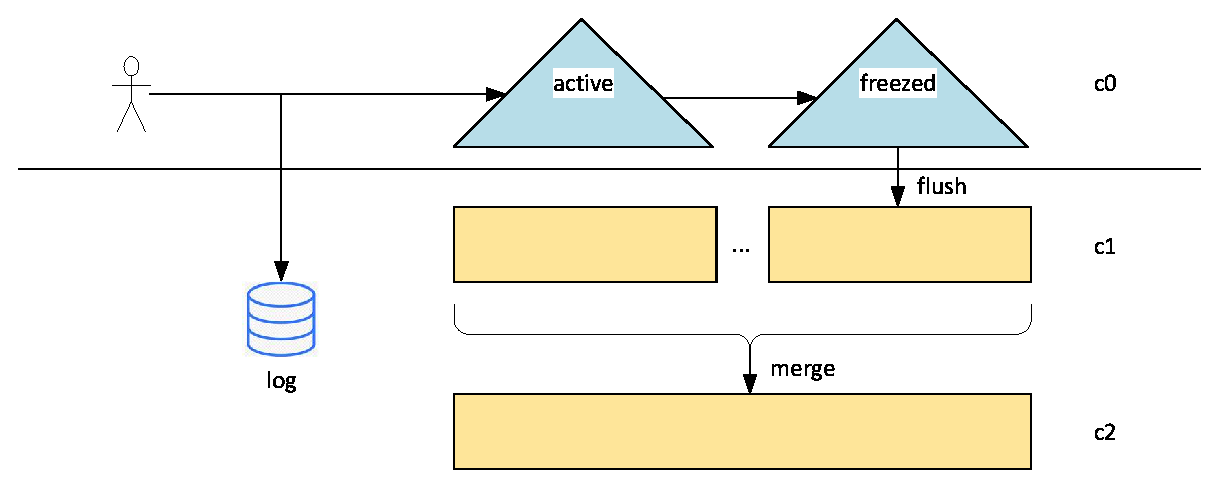
\includegraphics[width=\linewidth]{handout/img/2-lsm.eps}
    \caption{LSM-tree结构}\label{fig:2-lsm}
\end{figure}

LSM-tree\cite{o1996log}是这种思路的实现方案，数据到达，先写日志，然后在内存里排序，当容量超过阈值时，将这个排序结构凝固，然后flush到磁盘。按照这个方案，写入速度会极快，甚至在批处理场景下完全可以不写日志，出错后重启批处理即可。后面为了查询方便，启动一个后台进程，对写入数据做多路归并merge，将小块的有序数据规整为有序的更大块数据。

\subsection{leveldb存储格式}

leveldb\cite{GitHubgo38:online}是LSM结构的一个成熟实现，作者Jeff Dean在google有较长的工作经历，在从google退出后，开源了这个项目。leveldb是google多年kv存储开发经验的集大成作品，发布虽晚于HDFS，但它的成熟设计、高质量代码在发布后立即受到了广泛关注。

这里仅讨论leveldb的底层存储格式，它的架构留到下一章再介绍。

\begin{figure}[H]
    \centering
    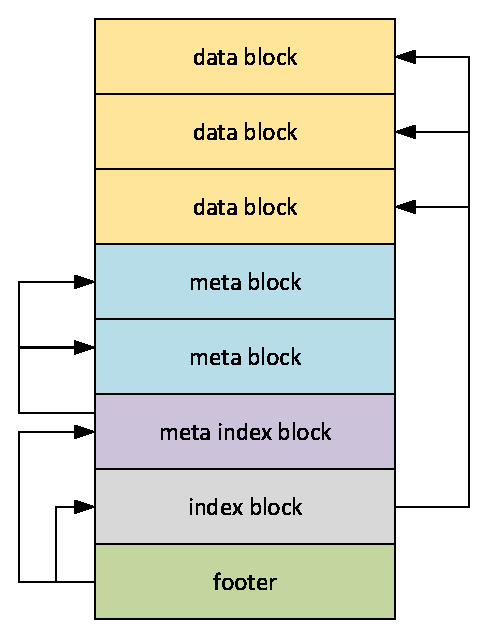
\includegraphics[width=0.5\linewidth]{handout/img/2-sstable.eps}
    \caption{sstable结构}\label{fig:2-sstable}
\end{figure}

leveldb将底层存储格式称为sstable，sstable的格式如\figurename\ref{fig:2-sstable}所示。它内部主要包含5个部分：

\begin{itemize}
    \item data block：存储实际的key-value数据记录。
    \item meta block：存储一些额外的元数据，如压缩算法、校验和等。
    \item index block：用于定位data block，给出每个data block的offset和size。
    \item meta index block：用于定位meta block，给出每个meta block的offset和size。
    \item footer：sstable访问入口，定长位于sstable文件尾部。
\end{itemize}

\begin{figure}[H]
    \centering
    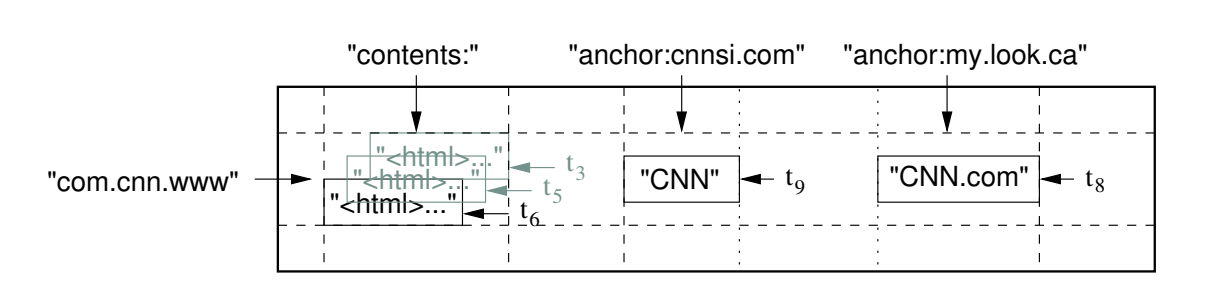
\includegraphics[width=\linewidth]{handout/img/2-kv.png}
    \caption{kv存储模型示例}\label{fig:2-kv}
\end{figure}

对sstable的访问是从尾部footer开始的，footer大小固定，内部有两个指针，分别指向meta index block和index block。如果寻找数据，则从index block开始，二分查找key所在的data block，然后从data block开始顺序查找。

sstable中，datablock和indexblock都是按照kv格式存储。kv存储的数据模型不再是关系型数据库的关系型模型，而是一种简单的键值对。kv模型相对于关系，它更简单，表达能力更强。以\figurename\ref{fig:2-kv}为例，批处理的爬回的页面以kv方式存储，url为www.cnn.com的页面，其网页内容存储在一个单元中。这个单元存放多个爬回的版本，这些版本以时间$t_3,t_5,t_6$作为key存储。这个例子中，anchor称为一个列族，按照锚点cnnsi.com、my.look.ca划分出不同的列，www.cnn.com对应的列族有不同的kv值。从这个例子来看，kv存储非常自由，列并不固定，允许嵌套。

\begin{exercise}
    如果用kv方式来存储一张关系表，采用列式存储，key可能重复多次写入。有没有可能采用key/value分离的方案，将表的一列分别存储？参考tdengine的存储模型提出解决方案。
\end{exercise}

sstable中的kv存储是将一列的多个kv对连续存储，这些kv对按照key顺序排列。由于key类型相同，并且临近kv对的key值相近，因此采用前缀压缩存储。每个kv对称为一个entry，在\figurename\ref{fig:2-prefix}中，key2要和前面的key1相比，表示共享了多少个字节，有多少字节的不同，然后给出不同部分以及value。

\begin{figure}[H]
    \centering
    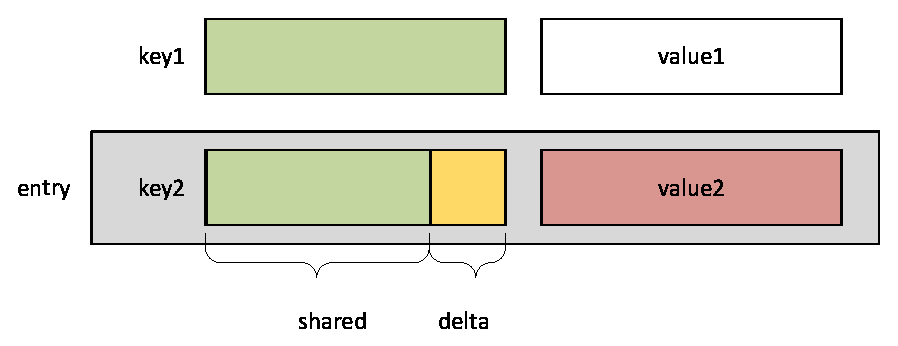
\includegraphics[width=0.8\linewidth]{handout/img/2-prefix.eps}
    \caption{kv前缀压缩示意图}\label{fig:2-prefix}
\end{figure}

leveldb在TableBuilder中创建一个sstable，datablock的格式如\figurename\ref{fig:2-block}所示。offset指向一个datablock，每个datablock的大小约为4KB，不一定对齐4KB。根据size找到datablock的尾部，尾部为num\_restarts、type、crc32，这几个字段都是固定大小。在num\_restarts之上是restarts[]数组，数组的每一项是固定大小的restart偏移量。

leveldb采用前缀压缩存储kv对，在TableBuilder构造datablock时，默认每16个kv对处理为一组，称为一个restart point。每个kv对的存储格式包含5个部分。shared\_bytes表示该kv对与restart point最前面的kv对共享的字节数，non\_shared\_bytes表示key中不同的字节数，value\_length表示value的长度，non\_shared\_key表示key中不同的部分，value表示value。

\begin{itemize}
    \item shared\_bytes (varint32): 表示key和前一个key共享的字节数。
    \item non\_shared\_bytes (varint32): 表示key中不同的字节数。
    \item value\_length (varint32): 表示value的长度。
    \item non\_shared\_key (bytes): 表示key中不同的部分。
    \item value (bytes): 表示value。
\end{itemize}

\begin{figure}[H]
    \centering
    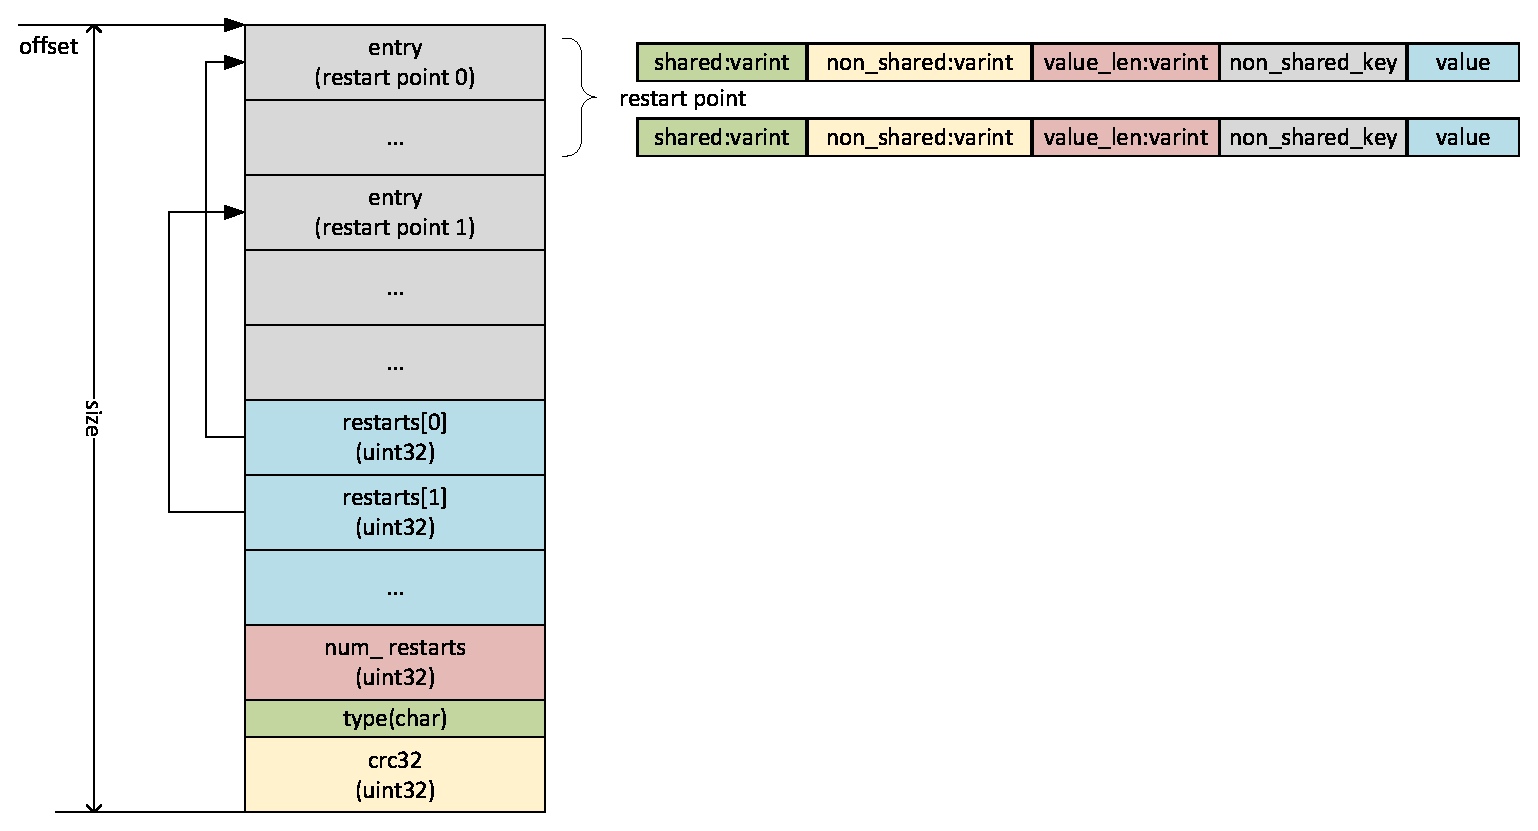
\includegraphics[width=1.2\linewidth]{handout/img/2-block.eps}
    \caption{data block格式}\label{fig:2-block}
\end{figure}

\begin{exercise}
    \figurename\ref{fig:2-block}展示的是datablock的格式，index block的格式呢？sstable中，indexblock可以有多个吗？sstable尾部footer，是否要包含indexblock的大小？
\end{exercise}
\begin{exercise}
    每个restart point最前面的kv对，key的shared\_bytes为多少？non\_shared\_bytes为多少？
\end{exercise}
\begin{exercise}
    关系型数据库中，一般在数据文件的头部放元信息。sstable中的footer包含元信息，为什么放在尾部？同样，num\_restarts也放在尾部，CRC32也放在尾部，这是为什么？
\end{exercise}
\begin{exercise}
    数据校验的方式有多种，有奇偶校验，crc校验，sstable为什么采用crc32？采用奇偶校验行不行？
\end{exercise}

整个datablock内存构建完成后，可以进一步使用snappy压缩，snappy压缩方案速度极快，压缩率中等。然后设置datablock尾部的type，表示为snappy压缩的block。

\section{实验}

本章设计三个实验，分别为聚集存储、堆存储和kv列式存储，前两个是关系型数据库的存储方案，最后一个是kv列式存储方案。

\subsection{聚集存储}

聚集存储实验主要参考innodb方案，数据文件分页，页面格式大致为\figurename\ref{fig:2-page}。聚集存储的页面，slots数组存放kv对的偏移量，这些偏移量按照key顺序排列，搜索以二分查找。使用key查找对应的记录，需要打开记录格式，比较key。

聚集存储的数据一般与主键索引合并存放，数据页面看成btree的叶子节点。每次新插入一条记录，可能会导致页面分裂，由于数据页面看成btree的叶子节点，数据页面分裂可能会引起btree调整。

以上是聚集存储相对于堆存储模型的劣势，但聚集存储带来的好处是，由于key相近的记录存放在相邻的页面，因此可以利用缓存预读，提高访问效率。也就是说，聚集存储以插入的代价换取了查找性能的提升。

\subsection{堆存储}

堆存储实验参考PostgreSQL的存储方案，堆模型将所有页面看成一个堆。当需要分配一个空闲空间，堆模型不会去按照key相近的原则去寻找页面，而是随意找到一个有足够空间的页面就好。

在堆模型的页面中，也安排slots数组，但是该数组不会以key顺序排列，它是作为rowid的间接索引，记录在页面内部不需要定位置，能够在页面移动，只要保证该记录在slots上的索引位置不动就好。如果记录在页面内位置固定，很难处理页面内部的碎片。

堆模型的btree树，它的指针是rowid，按照PostgreSQL的设计，rowid包含page\_number和slot\_number。page\_number表示记录所在的页面，slot\_number表示记录在页面中的偏移量。根据key在btree找到rowid，然后根据rowid再找到记录。

堆模型相对于聚集存储模型，插入速度快，并且对btree调整少，因此堆模型在插入操作频繁的场景下，性能更好。当记录被删除，堆模型页面slots可能会出现空槽位。

\subsection{kv列式存储}

kv列存实验主要参考leveldb方案。leveldb的原始设计中，key/value作为一个整体，存储在一个datablock中。如果kv模型表达关系表，key会存储多次，除非以除key外所有字段作为value。

观察到大多数应用中，每一列的类型都是相同的，并且排序后，相邻行一般数值接近。如果针对该列的类型做压缩，压缩率会非常高。本实验，要求在leveldb基础上，设计一种key/value分离的存储方案，将表中的key和value分别列式存储，可以参考tdengine、cassandra。


 % 2
\chapter{Index}

record存储在底层页面上，如果按照堆模型，要找到某个record，需要遍历整个页面，时间复杂度为$O(n)$，考虑到io非常慢，这个复杂度是难以接受的。一个完整的存储引擎，一般包括三部分的内容：底层存储组织、索引结构和缓冲管理。本章介绍索引结构，主要包括btree和lsm\cite{o1996log}结构。

\section{索引概念}

抽象上看，一个索引就是一个函数，给定key，输出record的位置。
$$
pos = f(key)
$$
将问题简化，假设一个堆模型上，record的位置不发生变化，如何表达这个函数$f(x)$？一个简单的方案是采用用数组记录每个record的位置，如\figurename\ref{fig:3-heap}所示。为了快速找到某个record的位置，需要将数组按照key顺序排列，然后以二分搜索在数组上定位，这个复杂度为$O(log(n))$。

\begin{figure}[H]
    \centering
    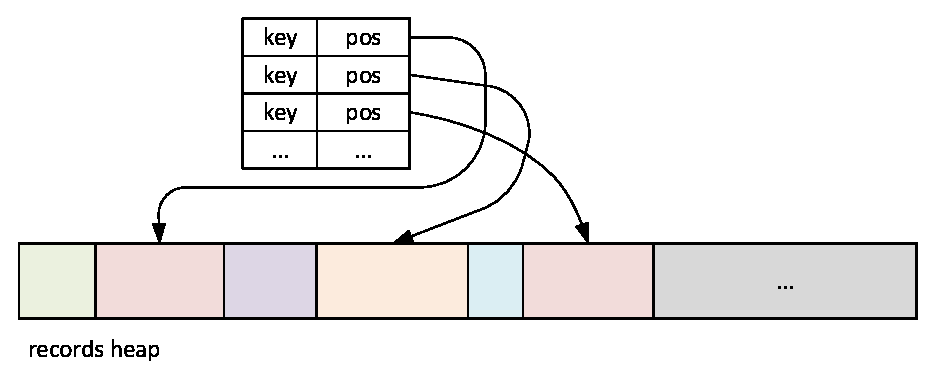
\includegraphics[width=0.8\linewidth]{handout/img/3-heap.eps}
    \caption{数组索引}\label{fig:3-heap}
\end{figure}

\begin{exercise}
    用数组来表示索引函数$f(x)$，有没有其它函数表示方案？
\end{exercise}

\subsection{稀疏索引与密集索引}

\figurename\ref{fig:3-heap}中每条记录在索引中都有一个对应的索引项，这个索引项记录了记录的key和记录的位置，这种索引称为密集索引。密集索引由于对每个记录都有索引项，整体尺寸比较大。索引结构会存放在磁盘上，要访问索引需要先调入内存，索引尺寸月大，访问时间也会增加，也不适合整体调入内存。

索引尺寸越小，io开销越小。同时考虑到并不总是要访问所有记录，所以只需要将部分索引项调入内存即可。因此，将\figurename\ref{fig:3-heap}分级，高层索引指向低层索引，低层索引指向记录，如\figurename\ref{fig:3-sparse}所示。高层索引称为稀疏索引，底层索引按需调入内存。

\begin{figure}[H]
    \centering
    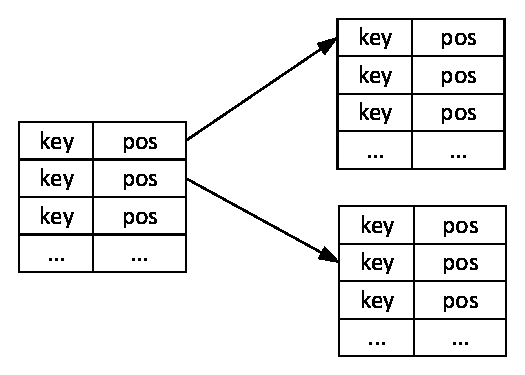
\includegraphics[width=0.5\linewidth]{handout/img/3-sparse.eps}
    \caption{稀疏索引}\label{fig:3-sparse}
\end{figure}

在\figurename\ref{fig:3-sparse}中，高层索引表项仍然是$(key, pos)$，与底层索引相同。实际上高层索引的key表示一个范围，在本文中都假设这个范围是左闭右开的区间$[key_{min}, key_{max})$。

\begin{exercise}
    分级索引下，$[key_{min}$和$key_{max})$对应于什么？最后一个索引项呢？
\end{exercise}

\begin{figure}[H]
    \centering
    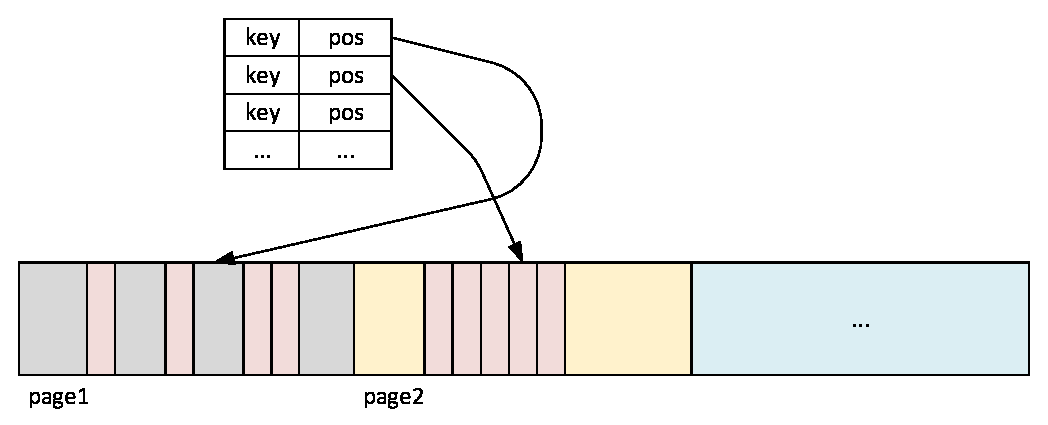
\includegraphics[width=0.8\linewidth]{handout/img/3-clustered.eps}
    \caption{聚集索引}\label{fig:3-clustered}
\end{figure}

\subsection{聚集存储与聚集索引}

\figurename\ref{fig:3-heap}中，底层存储模型为堆模型，如果采用上一章的分页模型，将key临近的记录放在临近的页面上，页面之间用指针连接起来，形成一个链表，页面的存储组织为聚集存储。考查聚集存储上的索引，key相近的记录会放在同一张页面上，页面实际上对应于一个连续的范围，因此聚集存储的索引称为聚集索引，聚集索引天然就是稀疏索引。

\begin{exercise}
    聚集存储的页面对应的范围一般不会相交，有没有相交的情况？
\end{exercise}
\begin{exercise}
    聚集存储中，两个页面临近，是指在位置上相邻吗？
\end{exercise}

实际系统中，不论是堆模型还是分页存储，都有一个问题，就是记录的位置会发生变化。如果记录的位置发生变化，索引就会失效。前述的数组方案只能用于记录位置不发生变化的情况。

\subsection{主索引与辅助索引}

主键的索引称为主索引，主索引的key是唯一的，每个记录都有一个主索引项。辅助索引的key可以重复，每个记录可以有多个辅助索引项。

\begin{figure}[H]
    \centering
    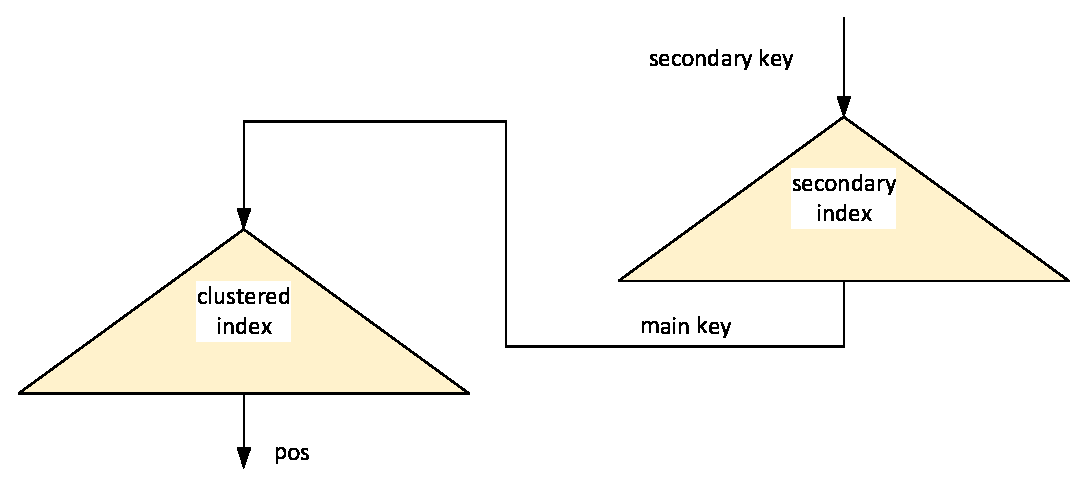
\includegraphics[width=0.8\linewidth]{handout/img/3-secondary.eps}
    \caption{聚集存储下的辅助索引}\label{fig:3-secondary}
\end{figure}

在聚集存储下，主索引是聚集存储，聚集索引给出rid一般是页面id。此时，辅助索引要检索记录的位置，需要先检索主索引，再根据主索引的结果检索记录，如\figurename\ref{fig:3-secondary}所示。

rid是一个重要概念，是记录id的简称，也可以称为rowid。聚集存储的rid一般是页面id，页面会根据key在页面的slots上确定记录在页面的偏移量。而在非聚集存储中，rid是pageid+slotid，slotid表示记录在slots数组上的下标。rid在不同系统上的称呼不同，PostgreSQL称为ctid，Oracle中称为rowid，但Oracle的rowid还会含文件号等信息。

btree里的指针实际上就是rid。

\section{btree}

索引本质上是一个搜索结构问题，在数据结构课程里有大把的搜索结构，如avl树、rbtree、hash表等。最终是btree在数据库系统中得到了广泛的应用，主要原因是btree更适合于磁盘存储。磁盘的访问单位是扇区，扇区在文件系统里组织为block，每次访问都以block为单位，btree天然适合这种访问方式。

\begin{figure}[H]
    \centering
    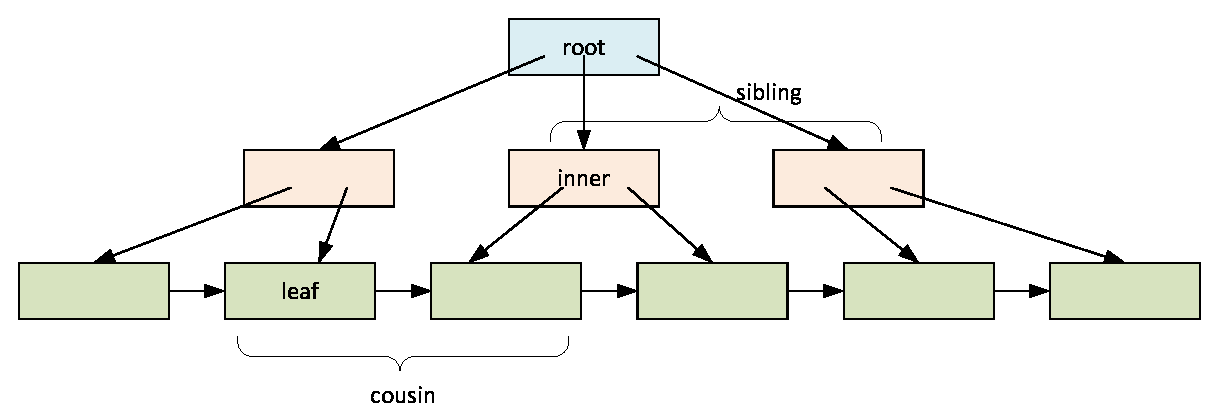
\includegraphics[width=\linewidth]{handout/img/3-btree.eps}
    \caption{btree结构}\label{fig:3-btree}
\end{figure}

btree是一种平衡多叉树，如\figurename\ref{fig:3-btree}所示，由根节点、内部节点和叶子节点构成。所有节点大小相同，在实现中，一般选择上一章的页面大小。同一个内部节点或者根节点的相邻子节点称为兄弟节点sibling，如果两个节点的父节点是兄弟节点，这两个节点称为堂兄节点cousin。

btree根节点和内部节点中，只包含key和指向子节点的指针，叶子节点包含key和指向记录的指针。并且，叶子节点之间形成一个单链表。

\begin{figure}[H]
    \centering
    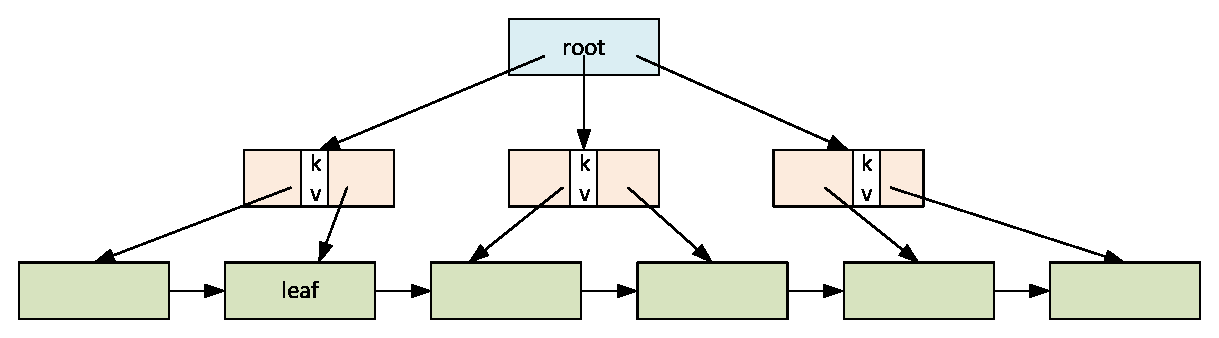
\includegraphics[width=\linewidth]{handout/img/3-btree2.eps}
    \caption{btree内部节点有kv}\label{fig:3-btree2}
\end{figure}
\begin{figure}[H]
    \centering
    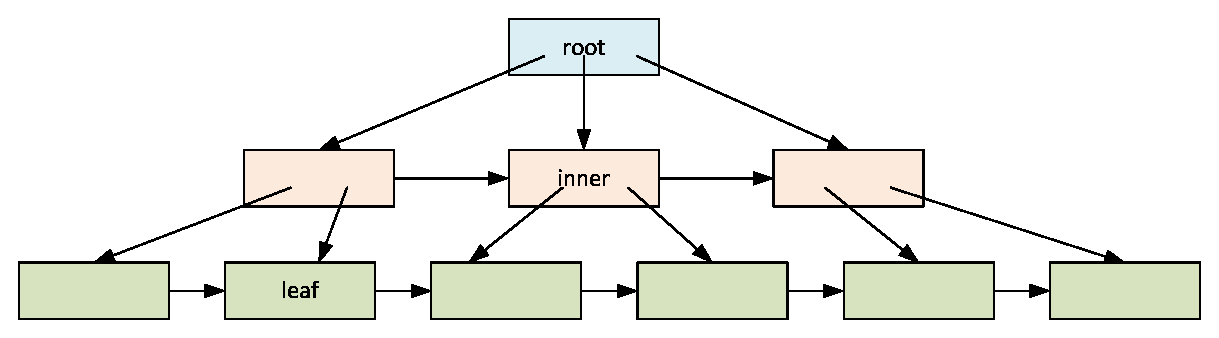
\includegraphics[width=\linewidth]{handout/img/3-bxtree.eps}
    \caption{b*tree内部节点有后继}\label{fig:3-bxtree}
\end{figure}

\subsubsection*{btree/b+tree/b*tree}

最早提出的btree虽然形如\figurename\ref{fig:3-btree}的结构，btree但叶子节点和内部节点上存储的是key+value+pos指针。本讲义中，btree实际指的是b+tree。b+tree与b*tree之间有细微区别，在b*tree中，内部节点之间也形成一个单链表。

b+tree的好处是，叶子节点、内部节点和根节点的结构完全相同，现代数据库中普遍采用b+tree作为索引。再次强调，本讲义中的btree是b+tree，而非最原始的btree。

\subsection{btree原理}

btree的叶子节点内部存储了key和pos指针，pos指针指向记录的位置，其中包括$n$个记录和$n$个记录的指针，同时还有一个指向下一个叶子节点的后继指针，如\figurename\ref{fig:3-leaf}所示。

\begin{figure}[H]
    \centering
    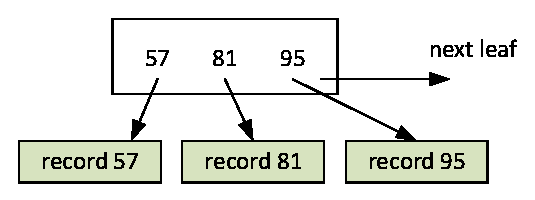
\includegraphics[width=0.5\linewidth]{handout/img/3-leaf.eps}
    \caption{btree叶子节点}\label{fig:3-leaf}
\end{figure}
\begin{figure}[H]
    \centering
    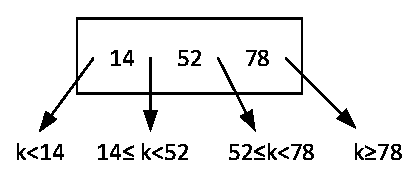
\includegraphics[width=0.4\linewidth]{handout/img/3-inner.eps}
    \caption{btree内部节点}\label{fig:3-inner}
\end{figure}

btree内部节点和根节点如\figurename\ref{fig:3-inner}所示，内部节点包含$n$个key和$n+1$个指向子节点的指针。在内部节点中，位于一个key左侧的指针表示小于这个key，位于key右侧的指针表示大于等于这个key。每个指针指向的是一颗子树，子树位于这个指针的key范围内。

\begin{figure}[H]
    \centering
    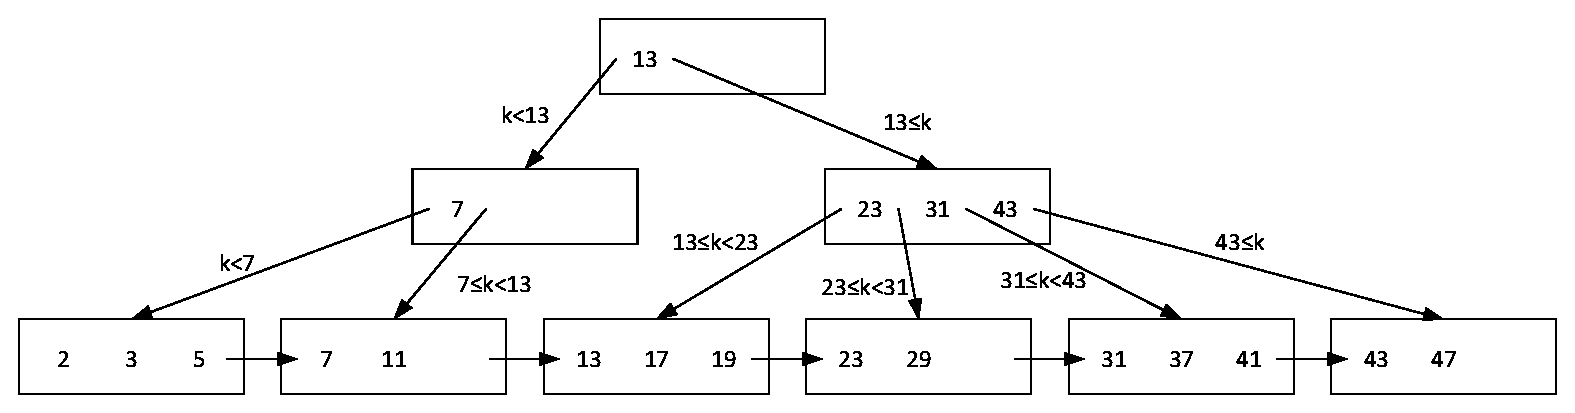
\includegraphics[width=\linewidth]{handout/img/3-btree3.eps}
    \caption{一颗完整的btree树}\label{fig:3-btree3}
\end{figure}

\figurename\ref{fig:3-btree3}是一颗完整的btree树，观察这颗树：
\begin{itemize}
    \item 观察叶子节点，除最左侧和最右侧节点外，所有叶子节点的范围是左闭右开的区间。
    \item 最左侧叶子节点是一个右开区间，最右侧叶子节点是一个左闭区间。
    \item 同理，每层中间节点的性质与叶子节点类似。
    \item 内部节点最左侧指针指向的范围需要父节点参与确定，除非该节点位于最左侧。
\end{itemize}

btree是平衡多叉树，所谓平衡是指节点的分布平衡，所有叶子节点都在同一层内。内部节点、叶子节点都要求容量过半，允许根节点容量低于一半。当key变长时，节点内包含的key和指针数目是变化的。很多教材都会采用固定长度的key来讲解btree，但要注意节点容量是变化的，或者说容量不是key的个数，而是占用节点存储尺寸。

\subsubsection*{查找}

在btree查找一个记录，很直观。从根节点开始，在根节点和内部节点上根据key确定要访问的子树，沿着子树下降，直到叶子节点。在叶子节点上，根据key确定要访问的记录。

在节点内部，使用二分搜索查找子树或者记录，查找的层数是树高，整体的时间复杂度是$O(\log n)$。

\begin{exercise}
    btree的性能一定比rbtree好吗？
\end{exercise}

实际系统中，可能在叶子节点上没有对应的记录，可能要返回小于该key的最大记录位置。并且，考虑到在插入和删除记录，需要使用查找操作来确定记录的位置，查找应该返回从根到叶子节点的整条搜索路径。

\begin{exercise}
    在\figurename\ref{fig:3-btree3}中，查找key为40的记录。
\end{exercise}

\subsubsection*{范围查找}

btree支持范围查找，这在数据库中是非常重要的操作。范围查找的方式是，先确定左边界，然后从左边界开始遍历，直到遍历到右边界。

\begin{example}
    假设执行如下SQL查询：
\begin{lstlisting}[style=verbose]
    SELECT * FROM R WHERE R.k > 40;
    SELECT * FROM R WHERE R.k >= 10 AND R.k <= 25;
\end{lstlisting}
第1条查询语句，从根节点开始，递归下降到叶子节点，找到41，然后向后枚举所有记录，过程如\figurename\ref{fig:3-lookup}所示。
\begin{figure}[H]
    \centering
    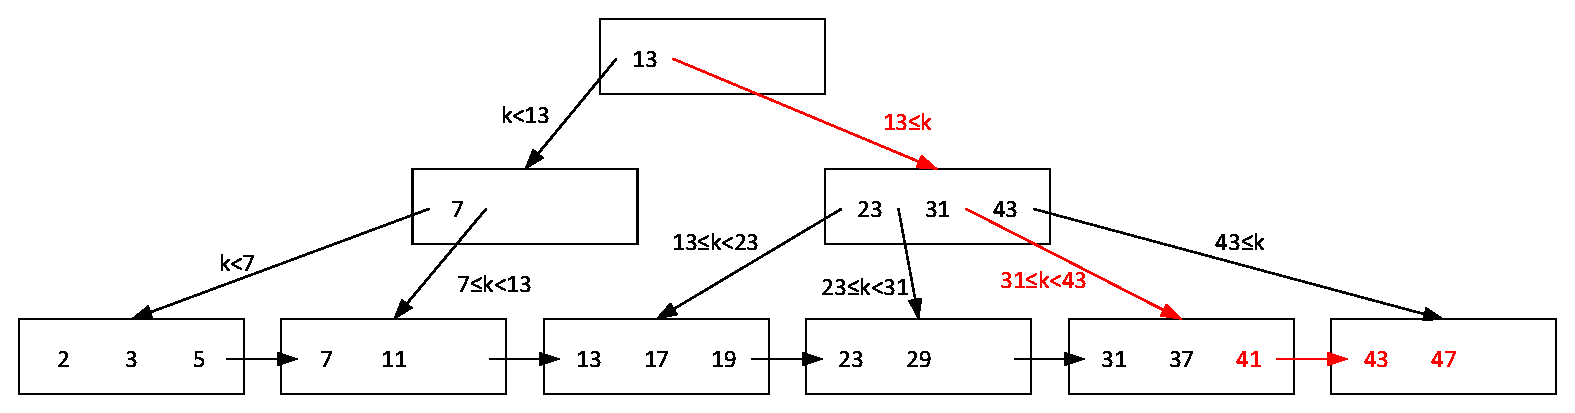
\includegraphics[width=\linewidth]{handout/img/3-lookup.eps}
    \caption{查找40后的记录}\label{fig:3-lookup}
\end{figure}
\end{example}

\begin{exercise}
    为什么btree的范围查找不需要确定右边界？
\end{exercise}
\begin{exercise}
    在\figurename\ref{fig:3-btree3}中，查找key为10到25的记录。
\end{exercise}

\subsubsection*{插入}

在btree中插入一条记录，需要先查找记录的位置，然后在叶子节点上插入记录。如果插入后导致节点容量超过上限，需要进行分裂。节点分裂，意味着多出了一个指针，需要在父节点上新增这个指针。这个过程是从叶子节点向根递归，直到根节点，如果根节点的容量不够，还需对根节点分裂，此时意味着树的高度增加了一层。

节点分裂的标准是，节点的容量超过上限时，分裂成两个节点，每个节点容量减半。实际系统中，由于key可能变长，容量是指节点的存储尺寸，而不是key的个数。并且，由于key变长，这种分裂可能并不一定会很均匀，但实际应用中问题不大。

\begin{exercise}
    证明key变长时，btree仍然是平衡的。
\end{exercise}

\begin{example}
    在\figurename\ref{fig:3-btree3}中，插入key为40的记录。首先在叶子节点上插入，叶子接点分裂如\figurename\ref{fig:3-insert1}所示：
\begin{figure}[H]
    \centering
    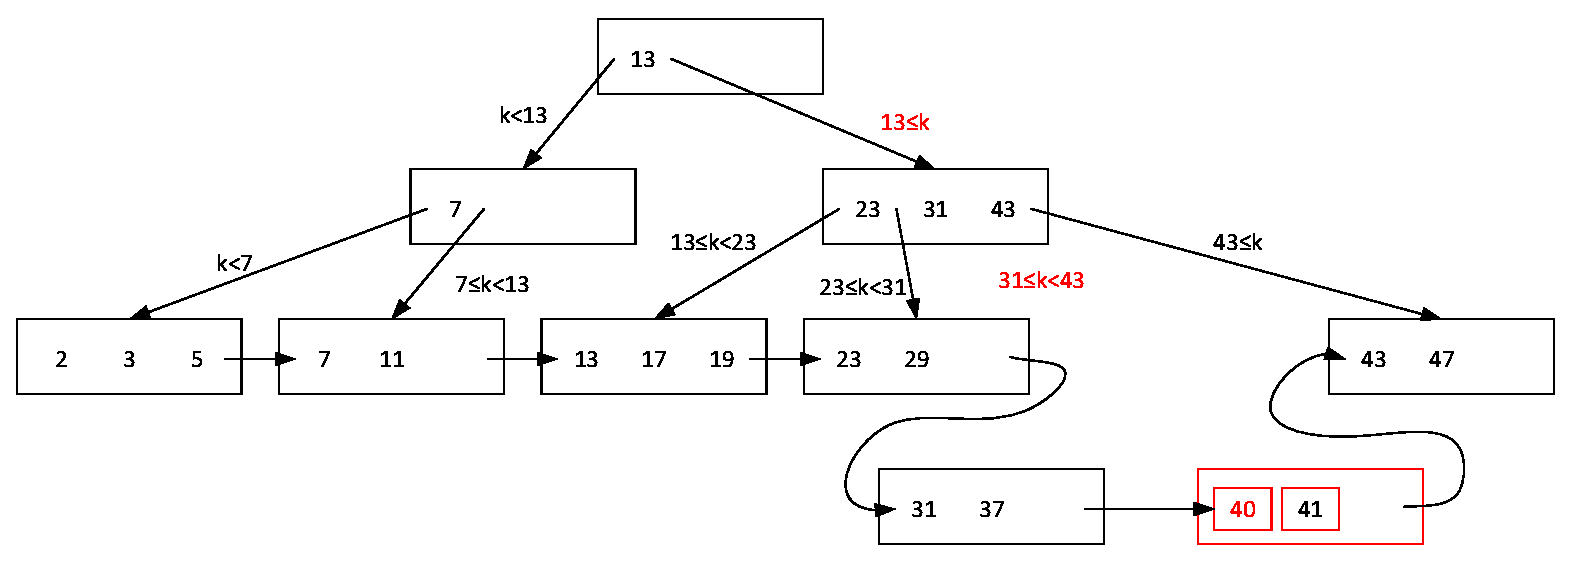
\includegraphics[width=\linewidth]{handout/img/3-insert1.eps}
    \caption{叶子节点分裂}\label{fig:3-insert1}
\end{figure}
新增叶子节点放在原叶子节点之后，然后需要递归向上插入新的指针。新增指针指向新节点最左侧的key，对应于\figurename\ref{fig:3-insert1}的40。这个40的key要在父节点上插入，如果父节点容量也超过上限，需要继续分裂。
\begin{figure}[H]
    \centering
    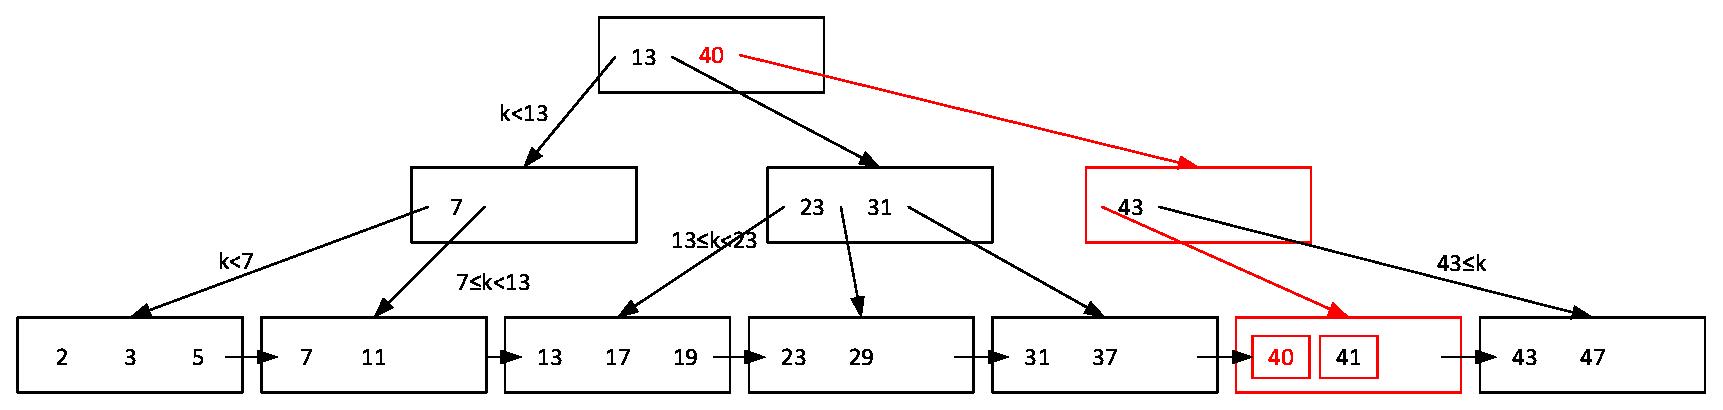
\includegraphics[width=\linewidth]{handout/img/3-insert2.eps}
    \caption{内部节点分裂}\label{fig:3-insert2}
\end{figure}
但是内部节点分裂不同于叶子节点分裂，新的内部节点需要将最左侧的key上移到父节点上，对应于\figurename\ref{fig:3-insert2}中的根节点。为什么不同？设想一下，4个key，5个指针，按照key分裂为2+2形式，2个节点会有6个指针。新内部节点上移，相当于带走了一个指针。
\end{example}

\begin{exercise}
    新增叶子节点为什么要放在右侧？同理，新增内部节点也需要放在右侧？
\end{exercise}

\subsubsection*{删除}

删除一条记录，需要先查找记录的位置，然后在叶子节点上删除记录。如果删除后导致节点容量低于下限，需要向临近的兄弟节点借，如果兄弟节点出借后，也低于下限，就需要将两个兄弟节点合并。

\begin{example}
    在\figurename\ref{fig:3-insert2}中，删除key为7的记录。删除7对应的记录后，叶子节点容量不够，需要向兄弟节点借记录。
\begin{figure}[H]
    \centering
    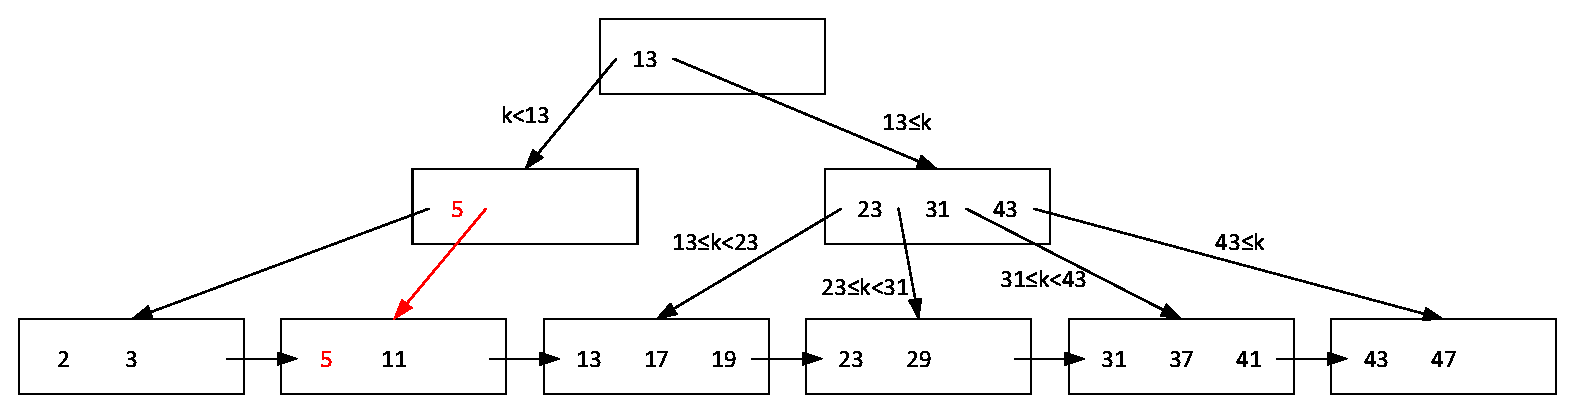
\includegraphics[width=\linewidth]{handout/img/3-delete.eps}
    \caption{删除7后的记录}\label{fig:3-delete}
\end{figure}
由于借到了5的记录，叶子节点的最左key发生变化，父节点的key也需要相应变化。
\end{example}

删除记录，导致叶子节点容量不够，向兄弟节点借记录。兄弟节点有两个，一个是左侧，一个是右侧。如果向左侧兄弟借，会改变节点的最左侧key，该叶子节点的指针对应的key也需要变化。借右侧兄弟节点，需要调整指向右侧节点的指针和key。

\begin{example}
    在\figurename\ref{fig:3-delete}中，删除key为11的记录。删除11对应的记录后，叶子节点容量不够，需要向兄弟节点借记录，如\figurename\ref{fig:3-delete2}所示。
\begin{figure}[H]
    \centering
    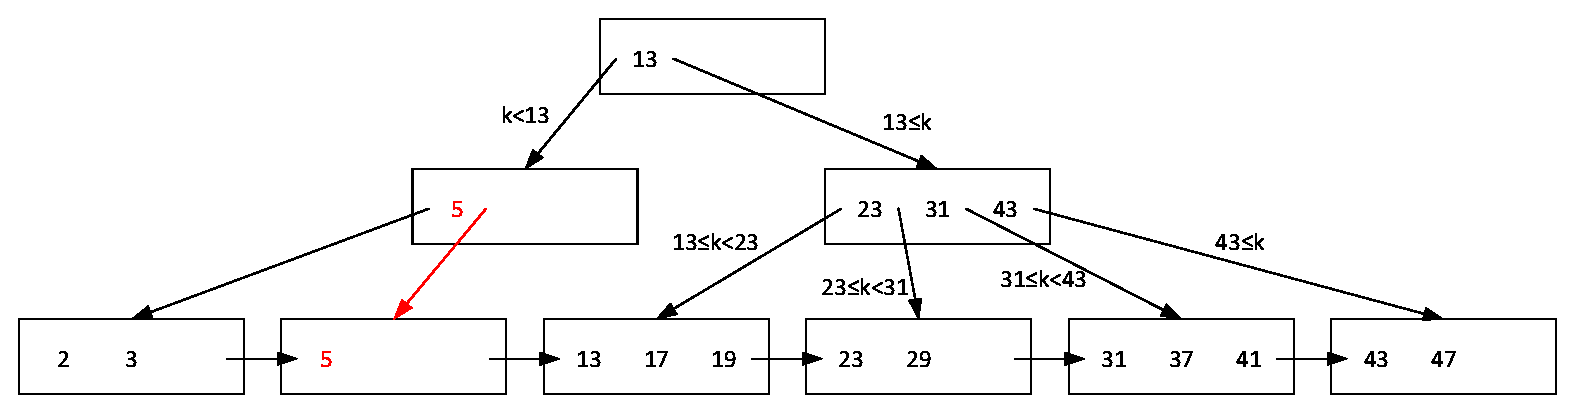
\includegraphics[width=\linewidth]{handout/img/3-delete2.eps}
    \caption{删除11后的记录-1}\label{fig:3-delete2}
\end{figure}
由于右侧没有兄弟节点，只能向左侧兄弟借记录，但左侧兄弟节点仍然不够，因此只能合并。合并后，删除该叶子节点，父节点中，指向该节点的指针和key也需要删除，对应于\figurename\ref{fig:3-delete3}所示：
\begin{figure}[H]
    \centering
    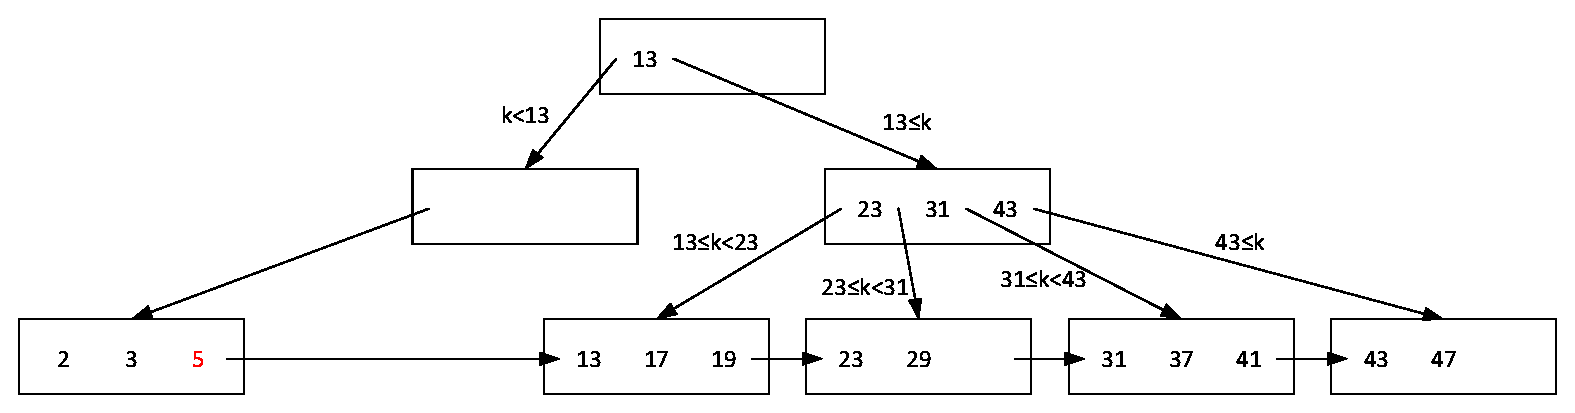
\includegraphics[width=\linewidth]{handout/img/3-delete3.eps}
    \caption{删除11后的记录-2}\label{fig:3-delete3}
\end{figure}
\begin{figure}[H]
    \centering
    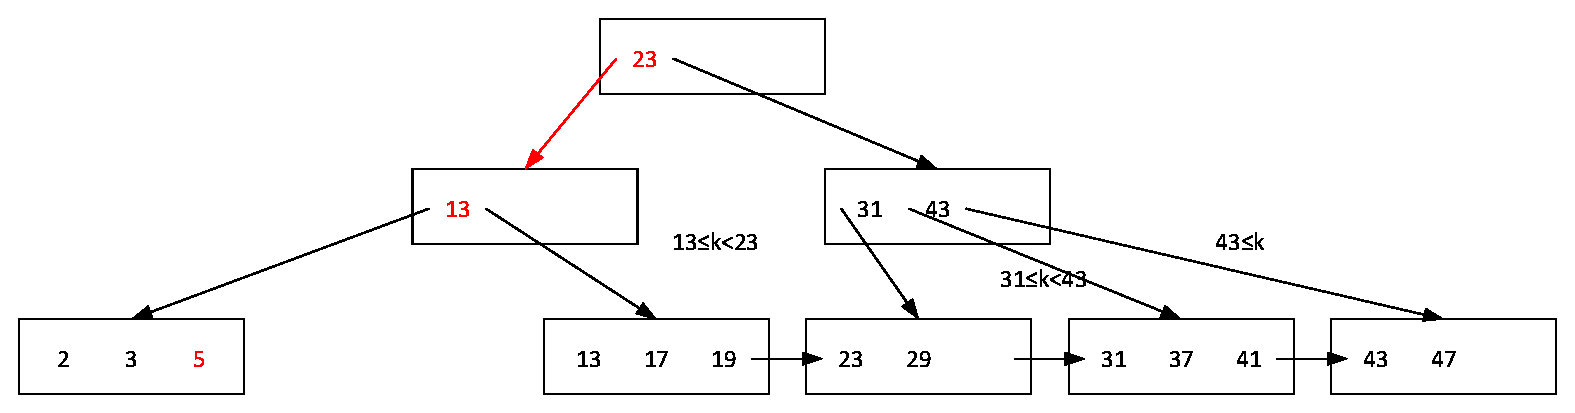
\includegraphics[width=\linewidth]{handout/img/3-delete4.eps}
    \caption{删除11后的记录-3}\label{fig:3-delete4}
\end{figure}
接下来考虑内部节点的情况。内部节点删除key和指针后，可能导致节点容量低于下限，需要向临近的兄弟节点借记录。如果借到的记录也低于下限，就需要将两个兄弟节点合并。内部节点借兄弟节点，也比较麻烦，需要同时调整父节点和兄弟节点，对应于\figurename\ref{fig:3-delete4}所示。
\end{example}

出借记录的情况比较复杂，这里需要总结一下。
\begin{itemize}
    \item leaf：叶子节点向兄弟节点借记录。确定截断位置，将内部节点的key改为截断位置后面的key。
\begin{figure}[H]
    \centering
    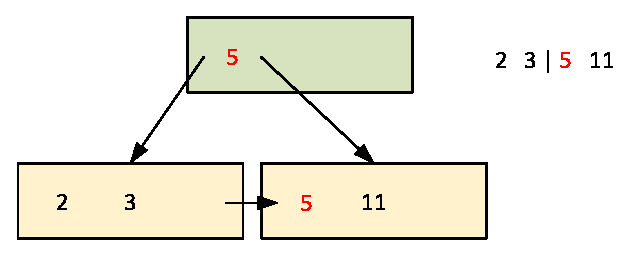
\includegraphics[width=0.5\linewidth]{handout/img/3-leaf-borrow.eps}
    \caption{叶子节点borrow}\label{fig:3-leaf-borrow}
\end{figure}
    \item inner：内部节点向兄弟节点借记录。两个内部节点一定是由某个key分隔，出借要将父节点的key考虑在内，如\figurename\ref{fig:3-inner-borrow}所示。确定截断位置，将父节点的key改为截断位置后面的key。
\begin{figure}[H]
    \centering
    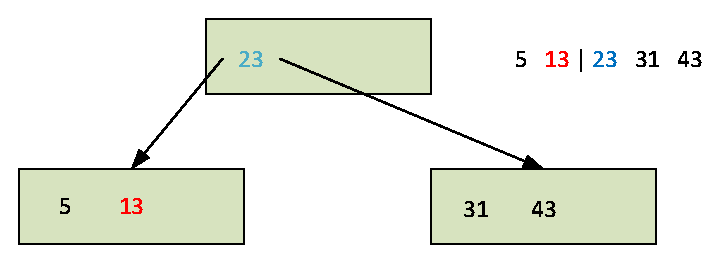
\includegraphics[width=0.5\linewidth]{handout/img/3-inner-borrow.eps}
    \caption{内部节点borrow}\label{fig:3-inner-borrow}
\end{figure}
\end{itemize}

\subsection{btree优化}

btree是数据库广泛采用的索引结构，对它的研究比较透彻，优化角度也比较多。

\begin{figure}[H]
    \centering
    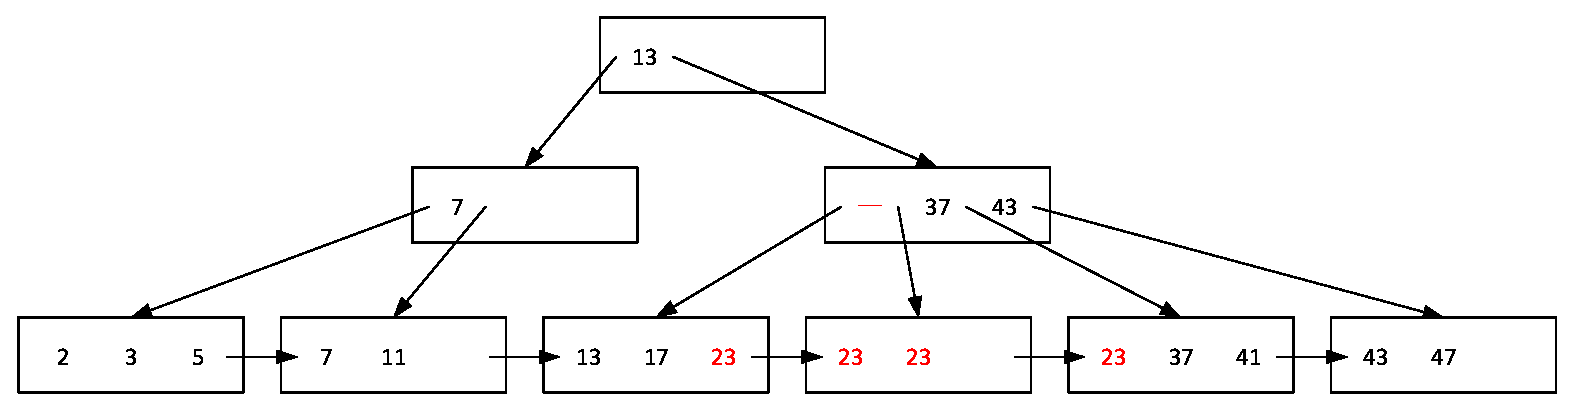
\includegraphics[width=\linewidth]{handout/img/3-duplicate.eps}
    \caption{重复键}\label{fig:3-duplicate}
\end{figure}

\subsubsection*{重复键}

主索引的key都是唯一的，但是辅助索引的key可以重复。重复键的处理方案可以有很多种，一种是直接将重复键的记录指针罗列在叶子节点中，对应于\figurename\ref{fig:3-duplicate}所示。这种方案的主要问题是，重复键过多，可能占用整个叶子节点，这会影响到内部节点的key如何处理。在\figurename\ref{fig:3-duplicate}中，23对应的key值在内部节点中用—来表示，意思是这个key值为null。当key值为null时，意思是整个叶子节点重复前面的key值。

\begin{exercise}
    如何表达key为—？或者说如何在数据库内部表达null？
\end{exercise}

另一种解法是利用记录格式来处理。重复键只能出现在辅助索引中，并且只能出现在辅助索引的叶子节点上，此时可以将这些指向重复键的记录指针顺序的排列在一条记录里。

\begin{figure}[H]
    \centering
    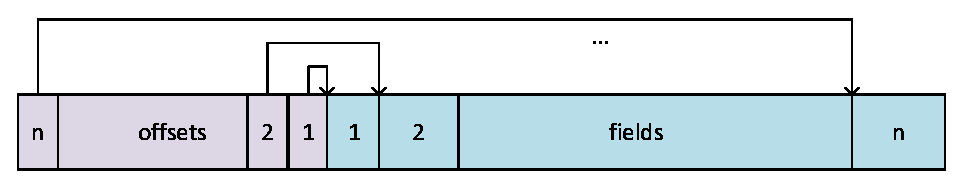
\includegraphics[width=0.8\linewidth]{handout/img/3-duplicate2.eps}
    \caption{将所有重复键的记录顺序罗列在一条记录}\label{fig:3-duplicate2}
\end{figure}

\subsubsection*{性能}

btree总是从根节点开始搜索，整个路径长度为树的高度。每次加载根节点都会产生一次io，io操作非常慢，一个很自然的方案是将根节点时刻缓冲起来。这样每次搜索就节省一次io，算总账的时候会节省很多io。

这个优化方案还可以更贪婪，将btree的高层都缓冲起来。这样每次搜索就节省更多的io。

\subsubsection*{页面格式}

btree的页面大小是上一章的页面大小，页面结构也与上一章相同。假设btree的节点要保存$n$个key，$n+1$个指针，一般是将$<key, ptr>$处理为一条记录，ptr是key右侧指针。页面尾部按照上一章介绍的slots数组维护。内部节点和根节点，最左侧的ptr使用页面头部的next指针存储。

\subsubsection*{前缀压缩}

由于btree中key是有序的，非常适合做前缀压缩。前缀压缩技术可以参考leveldb\cite{GitHubgo38:online}，在上一章也有过介绍。可以将整个page看成是leveldb的datablock，多个kv构成一组，取第1个key的前缀作为压缩前缀，后续key只需要存储与压缩前缀的差异即可。在page的尾部设置slots数组，维护各组的索引。

应用前缀压缩的前提是key要看成二进制字符串，leveldb中简单地用memcmp比较key。在关系数据库中，许多系统先经过collation校对后，再按照二进制字符串比较。

\subsubsection*{top-down策略}

节点分裂从叶子节点开始，向上递归分裂，直到根节点。这个过程与搜索过程相反，在latch节点时，容易出现死锁。可以先计算需要分裂的高度，然后从上向下分裂，分裂完毕后，再插入新记录。

同理，在删除记录时，也应该先计算需要合并的高度，然后从下向上合并或者出借。

\subsubsection*{延迟合并}

删除记录，会导致记录出现在不同的叶子节点或者内部节点，为保证搜索路径的正确性，必须使用拍它的latch，会阻塞其他线程的搜索。

有些系统假设表总是膨胀的，在删除记录后不会立即合并节点，也不主动向兄弟节点借记录。——这种方案可能会出现空节点。

\subsection{范围锁}

在后文介绍事务并发时，会使用范围锁来解决幻读问题，这里简单描述一下幻读问题。

假设系统运行在Read Commited, RC隔离级别及以下。有一张表phantom\_test，它有一个主键列id。两个事务a和b，交替执行以下操作：
\begin{lstlisting}[style=verbose]
-- 事务a第一次查询
BEGIN;
SELECT * FROM phantom_test WHERE id > 3 AND id < 8 FOR UPDATE;
-- 结果: id=5 (Bob)

-- 事务b
BEGIN;
INSERT INTO phantom_test VALUES (6, 'David');
COMMIT;

-- 事务a第二次查询（同一事务内）
SELECT * FROM phantom_test WHERE id > 3 AND id < 8 FOR UPDATE;
-- 结果: id=5 (Bob), id=6 (David)
COMMIT;
\end{lstlisting}

在上面的例子中，事务a第一次查询id大于3小于8的记录，结果只有id为5的记录。然后事务b插入了id为6的记录。事务a第二次查询id大于3小于8的记录，结果有id为5和6的记录。这就发生了幻读问题。

在后文的锁方案中，要杜绝幻读的发生，需要使用范围锁，即对查询的范围加锁，防止其他事务在这个范围插入记录。

\subsubsection*{区间范围}

WHERE语句使用的条件称为谓词predicate，就是限定词，谓词逻辑中使用限定词为$\forall, \exists$，SQL里使用的限定词要更复杂一些。谓词在最后被处理为一个或多个范围，这些范围的开闭有四种情况，如\figurename\ref{fig:3-gap}所示。

\begin{itemize}
    \item $[a, b]$：闭区间，包含a和b。
    \item $(a, b)$：开区间，不包含a和b。
    \item $[a, b)$：闭区间，包含a不包含b。
    \item $(a, b]$：开区间，不包含a包含b。
\end{itemize}

\begin{figure}[H]
    \centering
    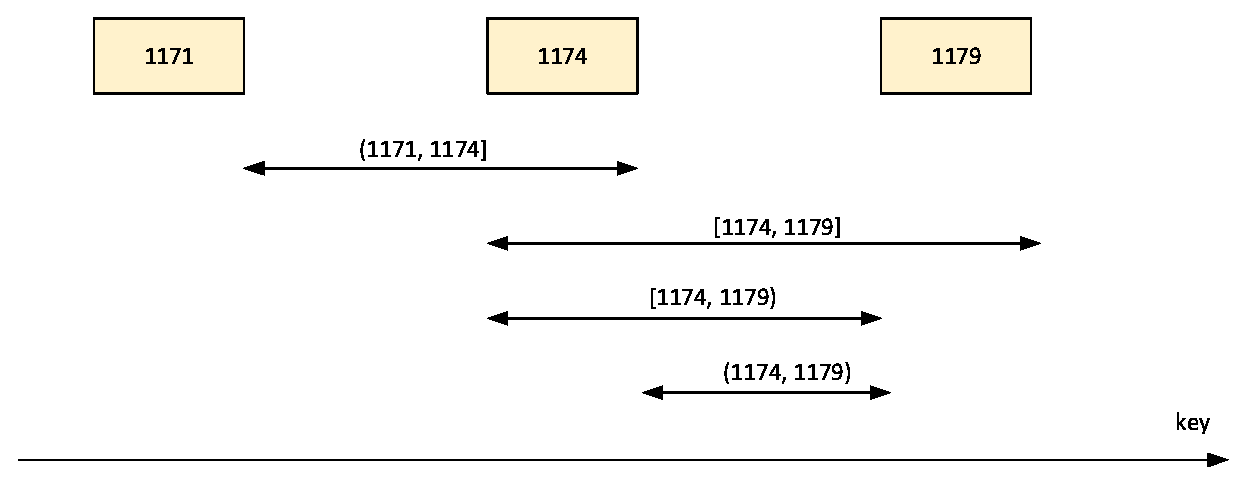
\includegraphics[width=0.8\linewidth]{handout/img/3-gap.eps}
    \caption{各种区间范围}\label{fig:3-gap}
\end{figure}

\subsubsection*{锁表}

在下一章会更详细介绍锁表，锁表是一个内存结构，一般用hash表构建。给定一个key，会先在锁表中查找是否有对应的锁。如果没有，就创建一个新的锁。如果有，则返回key对应的锁。\figurename\ref{fig:3-locktable}的锁表是一个点锁表，还不支持范围锁，接下来要扩展这个结构支持范围锁。

\begin{figure}[H]
    \centering
    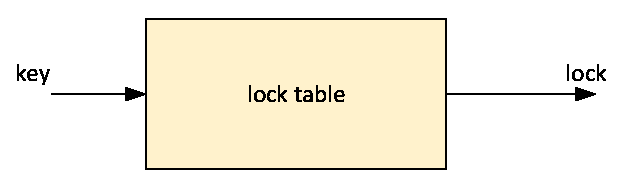
\includegraphics[width=0.6\linewidth]{handout/img/3-locktable.eps}
    \caption{锁表示意图}\label{fig:3-locktable}
\end{figure}

\subsubsection*{gap锁}

WHERE条件的谓词，可以直接处理为锁。每次想要获取锁时，先执行一下这个谓词，如果返回为true，就获取锁。但这种方案开销巨大，所有事务都必须无差别执行一遍谓词。解决方案是将这个谓词范围映射到btree的叶子节点上，在每个叶子上维持一个局部的小范围锁，如\figurename\ref{fig:3-gap2}。

每个btree叶子节点对应于一个锁管理结构，它管理叶子上的所有gap锁，包括点锁。这个管理结构以叶子节点的指针为key，注册到锁表。当搜索到叶子节点，就查找锁表获取这个结构。

\begin{figure}[H]
    \centering
    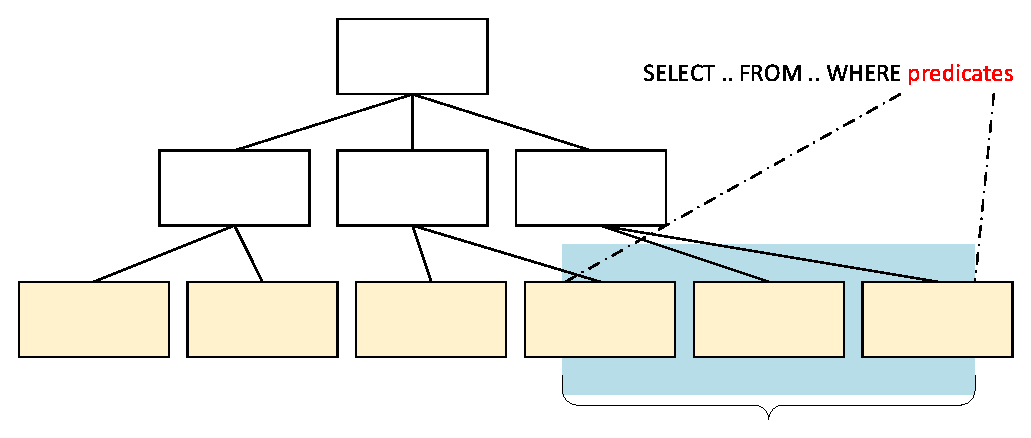
\includegraphics[width=\linewidth]{handout/img/3-gap2.eps}
    \caption{谓词映射为gap锁}\label{fig:3-gap2}
\end{figure}

\begin{exercise}
    gap锁为什么不在中间节点和内部节点上实现？
\end{exercise}

称叶子节点上的锁管理结构为leaf lock manager，它使用一个链表管理所有gap锁，需要加锁时要逐个测试这些gap锁。为了加快测试，可以将这个链表组织成一个区间树，每个区间对应一个gap锁。另外，为了判断是否加锁，使用bitmap来标记叶子上每个区间是否加锁。

\begin{figure}[H]
    \centering
    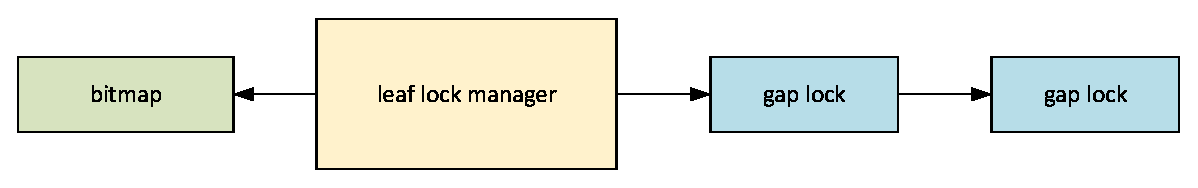
\includegraphics[width=\linewidth]{handout/img/3-leaflock.eps}
    \caption{叶子节点上的gap锁}\label{fig:3-leaflock}
\end{figure}

当使用bitmap来判断一个key是否落入某个区间时，实现上有些问题。gap锁的区间与叶子节点上的记录区间并不对齐，如\figurename\ref{fig:3-interval}所示。\figurename\ref{fig:3-leaflock}里的bitmap是用slots[]数组来标定，因此借用bitmap来判断是否加锁可能会出现误报，需要进一步使用链表来确定是否加锁。

\begin{exercise}
    为什么用slots[]数组来标定gap锁的区间？
\end{exercise}
\begin{exercise}
    如果使用gap树而非链表，是否可以省略掉bitmap？
\end{exercise}

\begin{figure}[H]
    \centering
    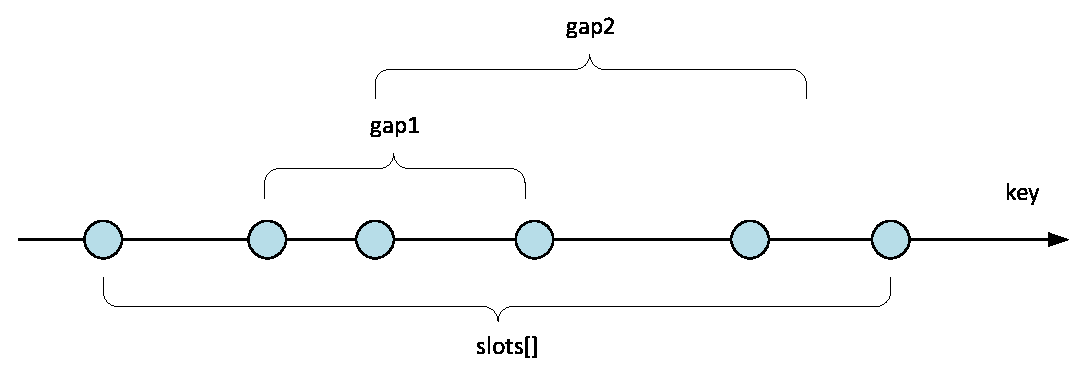
\includegraphics[width=\linewidth]{handout/img/3-interval.eps}
    \caption{gap与slots[]数组不对齐}\label{fig:3-interval}
\end{figure}

\section{skiplist}

跳表是kv存储中最常见的数据结构。kv存储一般采用append追加模型，数据写入后不再修改，这种模型与传统关系数据库中读写平衡的设计不同。kv存储的索引结构分为两部分，一是活动内存结构，二是持久化结构。活动结构用于索引未落盘的数据，参考\figurename\ref{fig:2-lsm}。持久化结构用于索引已落盘的数据，由于不会改变，就是有序数组，如\figurename\ref{fig:3-heap}。

leveldb是一个成熟的kv存储引擎，它的活动索引为跳表。之所以选择跳表，有几方面的原因：一是跳表是一写多读的lockfree结构，对多核系统支持较好。二是跳表天然支持范围查询，这在kv存储中是一个重要的功能。三是跳表的实现比较简单，容易理解和维护。四是跳表一开始就要设定容量，而在kv存储中，这不是问题。

\subsection{跳表结构}

跳表需要在内存中动态构建，它的基础数据结构是单链表，为了加快查询，它概率的在某些节点上建立多层的后向指针。

跳表结构如\figurename\ref{fig:3-skiplist}，head是一个多层的后向指针，初始化指向null，n是跳表中的节点数目。表中的节点除了存储数据外，还带有随机数目的层，每层指向同层的后继节点。这个随机层数与该节点插入时n的数目有关，当一个节点插入时，它取的层数服从均匀分布$l \sim U(1, \lfloor \log_2(n) \rfloor)$，在实现中这个$\lfloor \log_2(n) \rfloor$很容易计算，只需看n的哪个高位是1即可。

在levelDB的代码中，跳表节点表示如下。next是变长的一个原子指针数组，可以原子的方式修改指针。key是搜索键，结构中只定义了1个指针长度，需要在该节点构造时临时确定这个数组的大小。
\begin{lstlisting}[style=c++]
template<typename Key, class Comparator>
struct SkipList<Key,Comparator>::Node {
    Key const key;
    port::AtomicPointer next_[1];
};
\end{lstlisting}

\begin{figure}[H]
    \centering
    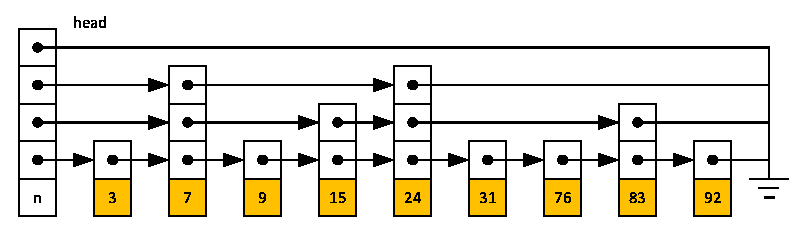
\includegraphics[width=\linewidth]{handout/img/3-skiplist.eps}
    \caption{跳表结构}\label{fig:3-skiplist}
\end{figure}

leveldb的跳表是一写多读的，只能有一个线程写入，原因是跳表是lockfree的，如果多写会丧失这些特性。leveldb采用c++实现，不支持删除操作。在leveldb实现中，节点分配使用了arena内存池，所以跳表节点没有析构函数。

\begin{exercise}
    加载一个\figurename\ref{fig:2-block}的sst文件，是否还需要构建跳表？
\end{exercise}
\begin{exercise}
    分析leveldb源码中，arena内存池是如何实现的？
\end{exercise}
\begin{exercise}
    跳表的容量如何确定？可不可以动态修改？
\end{exercise}

\subsection{功能}

跳表的搜索复杂度为$O(\log n)$，插入复杂度为$O(\log n)$，性能不弱于rbtree、btree。

\subsubsection*{查询}

跳表查询从head开始，从高层向底层迭代：1)~当碰到后继指针为null，向底层迭代；2)~如果后继节点的key比查询的键大，向下层迭代。\figurename\ref{fig:3-skiplist2}是查询9的例子。

\begin{figure}[H]
    \centering
    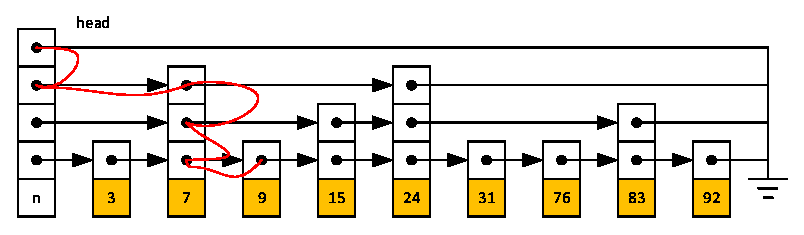
\includegraphics[width=\linewidth]{handout/img/3-skiplist2.eps}
    \caption{查询9的例子}\label{fig:3-skiplist2}
\end{figure}

在跳表上做范围查找，也是容易的，首先定位起始的节点，然后沿着最底层向后枚举即可。

\subsubsection*{插入}

在跳表上插入，首先要找到小于等于键的最大位置，然后分配节点，准备插入。由于新分配的节点可能有多层，为了将多层引入跳表，需要在定位插入位置时，保存所有层次的前驱节点。自上而下先初始化指向后继节点，然后自下而上修改前驱节点指向新增节点。

\begin{figure}[H]
    \centering
    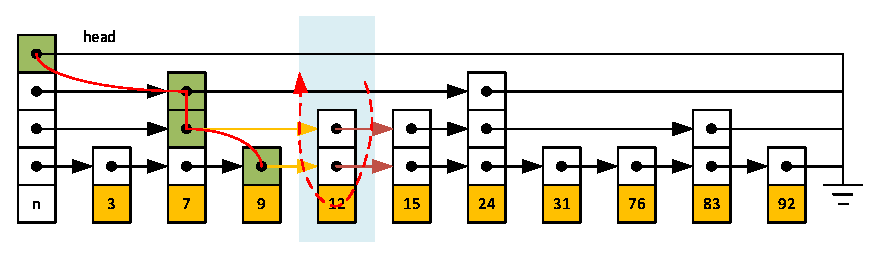
\includegraphics[width=\linewidth]{handout/img/3-skiplist3.eps}
    \caption{跳表插入}\label{fig:3-skiplist3}
\end{figure}

如\figurename\ref{fig:3-skiplist3}，要插入一个新节点12，先保存所有搜索路径。然后随机分配了一个2层的节点，自上而下先设置12节点的后继指针，然后修改前驱指针指向12。

\begin{exercise}
    跳表为什么不支持删除操作？还是leveldb里不支持？leveldb为什么不支持删除？
\end{exercise}
\begin{exercise}
    分析一下，跳表能否支持多写多读？
\end{exercise}

\section{rtree}

关系数据库的索引都是一维索引，实际的应用中存在着多维索引的需求。在诸如地理信息系统这样的应用中，数据按照二维或三维组织，这个时候就需要根据多维索引查找。

但是，多维索引的数据模型与一维索引的数据模型不同，如图\ref{fig:3-map}，地图上的图元有点、线、面的形式。点表示一个位置，线可能是一条道路，面可能是一栋大楼，线和面可以是任意形状的，例如道路可以是曲线，大楼可能是异形的。

地理信息系统GIS的数据模型与关系数据库的表不同，需要在SQL语言基础上做一些扩展，增加如下查询方式：
\begin{enumerate}
    \item 范围查询。给定任意形状的范围，搜索哪些图元在这个范围中。
    \item 邻居查询。给定一个图元，查找最近的图元。
    \item 定位查询。给定一个图元，定位包含该图元其它图元有哪些。
\end{enumerate}

空间索引是对存储在介质上的数据位置信息的描述，用来提高系统对数据获取的效率。空间索引的设计需要适应它的应用方式与图元的特性，例如电子地图需要由粗到细的刻画图元，图元的形状可能是任意的，rtree就比较合适。而在向量数据库中，由于维度很高，目标多为点且稀疏，用rtree来描述就不太合适。

\begin{figure}[H]
    \centering
    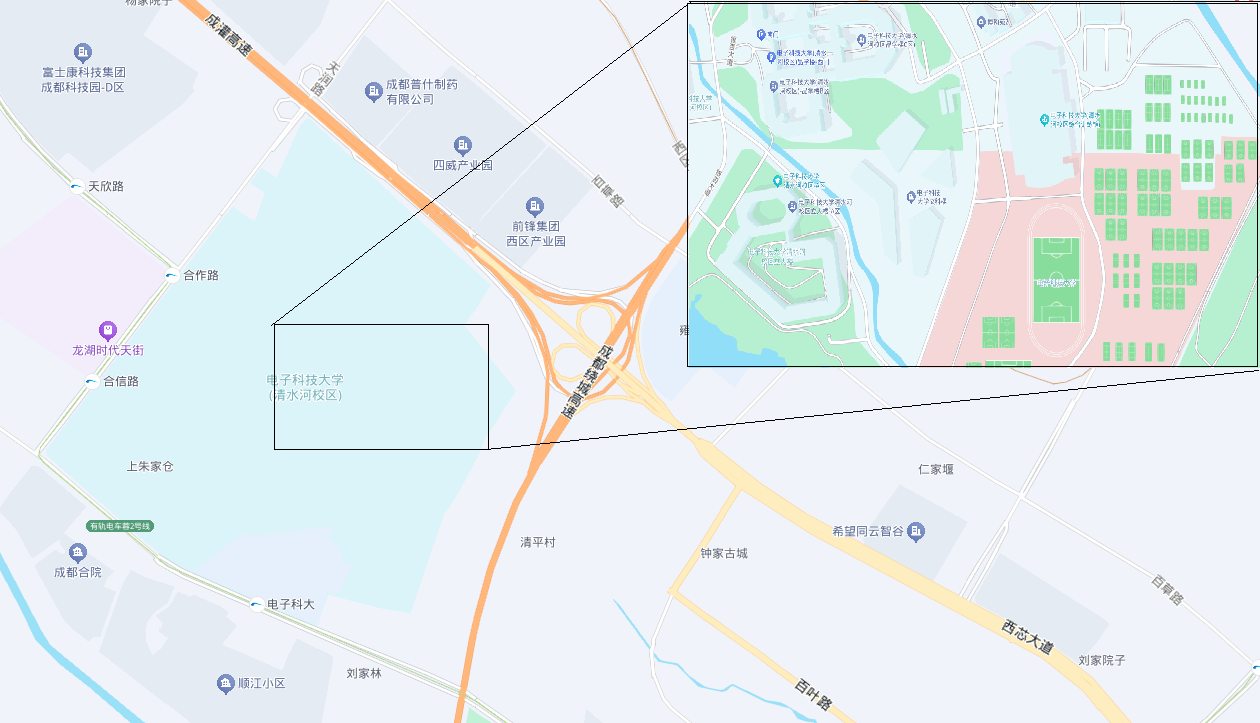
\includegraphics[width=\linewidth]{handout/img/3-map.png}
    \caption{二维地图与缩放}\label{fig:3-map}
\end{figure}

\subsection{rtree原理}

在rtree中，点、线、面使用bounding box来统一表示，如\figurename\ref{fig:3-rtree1}所示。在这个视场内，bounding box是最小的图元单位，它们之间可能彼此相交或者包含。在电子地图中，图元存放了对应的形状、坐标等信息。

\begin{figure}[H]
    \centering
    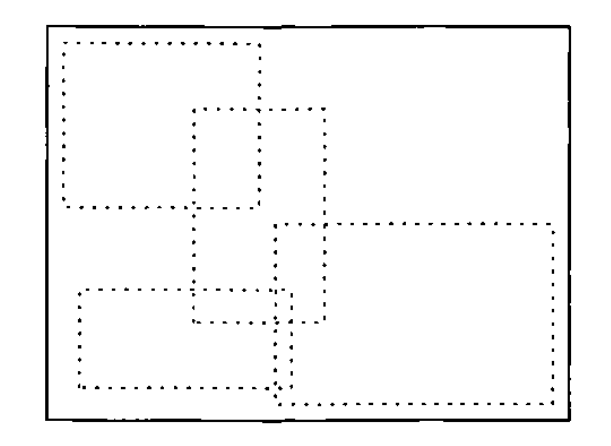
\includegraphics[width=0.6\linewidth]{handout/img/3-rtree1.png}
    \caption{bounding box示意图}\label{fig:3-rtree1}
\end{figure}

接下来需要考虑的是如何组织这些bounding box，以方便地进行范围查询。rtree的思路是在底层bounding box基础上，使用多个bounding box的并充当更高层的bounding box。通过分层的bounding box，就可以将视场分为多个区域，每个区域下会有多个图元。

\begin{figure}[H]
    \centering
    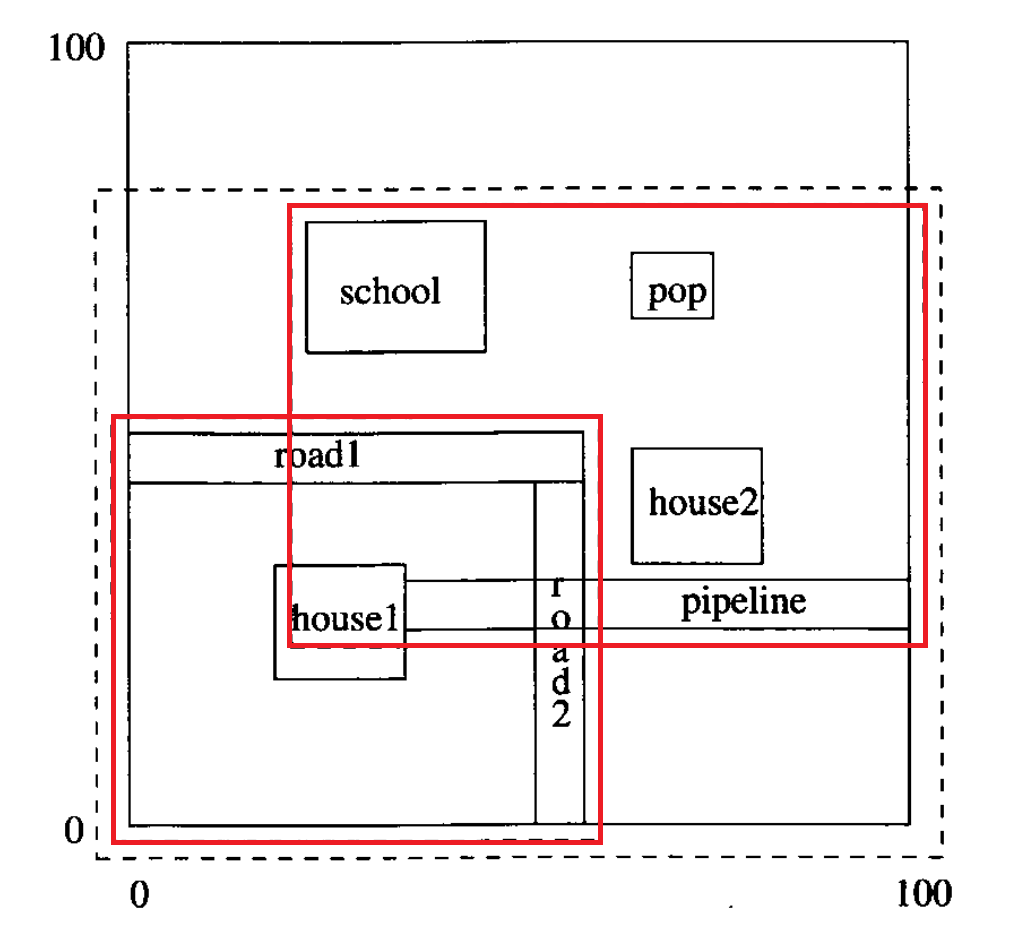
\includegraphics[width=0.6\linewidth]{handout/img/3-rtree2.png}
    \caption{rtree分层}\label{fig:3-rtree2}
\end{figure}

\subsection{rtree树}

rtree是一种空间索引数据结构，它模仿btree是一个多叉树，以固定大小的页面为节点。每个节点对应于一个区域，或者说是一个bounding box。rtree也分为根节点、内部节点、叶子节点。叶子结点上包含图元，其对应的矩为所有对象的外包矩形，非叶结点的矩形为所有子结点矩形的外包矩形。

\section{倒排索引}

在通常的应用中，我们使用key来访问索引，通过索引找到key对应的内容。倒排索引inverted index则相反，使用部分内容来找到包含该内容的所有key。

\begin{figure}[H]
    \centering
    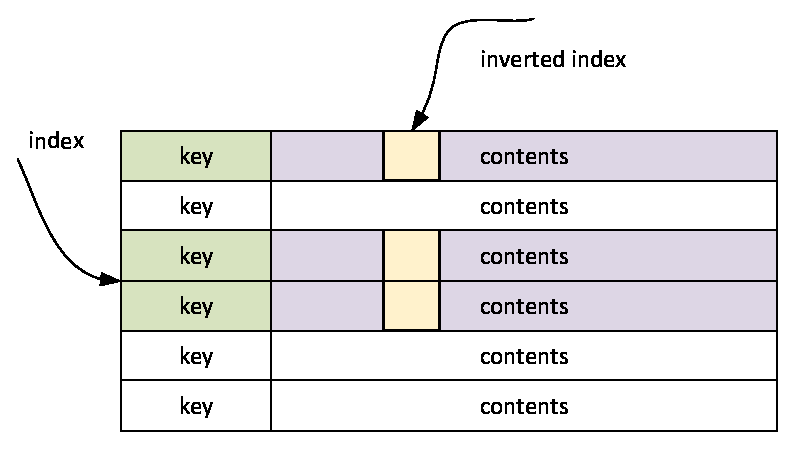
\includegraphics[width=0.6\linewidth]{handout/img/3-inverted.eps}
    \caption{倒排索引}\label{fig:3-inverted}
\end{figure}

倒排索引经常使用在全文检索中，例如搜索引擎。在搜索引擎中，用户输入一个查询字符串，搜索引擎需要找到包含该字符串的所有文档。倒排索引可以将每个文档中的每个单词作为key，将包含该单词的所有文档作为value，构建一个倒排索引。

\begin{exercise}
    搜索引擎的工作原理是怎样的？在搜索引擎中输入一个关键字，搜索引擎是象数据库一样即时查找的吗？
\end{exercise}

\subsection{标签}

在个人博客等应用中，经常对文章或者照片添加标签，例如“技术”、“生活”、“工作”等。用户可以根据标签来查找自己感兴趣的内容。标签索引就是用来支持这种功能的索引。

标签要看成对象的一种属性，根据标签来查找对象，实际上也是一种倒排索引，因为标签是对象的属性。但是标签应用中，并不需要象搜索引擎那么大型，因为标签的数量通常是比较少的，并且应用中很少有标签删除操作。

\subsubsection*{基于bitmap的标签系统}

将对象用id整型来表示，要构造标签索引，需要为每个标签维护一个bitmap，bitmap的每个位表示对应对象是否有该标签。id空间比较大，为了保存bitmap可以采用roaring压缩方案。

\begin{exercise}
    构思一个标签系统，支持添加标签、根据标签查找对象。
\end{exercise}

\subsubsection*{kv标签}

博客应用中，文章打的标签是tag类型。有些应用中，标签还可以带value，例如在iot设备中，某个检测点带的标签为position=32，意思是标签position的value值为32。 % 3
\chapter{Buffer and Schema}

本章介绍缓冲管理与schema设计。Schema部分的内容是一个独立的部分，并不属于存储引擎，放在此处是为了章节的平衡。

\section{缓冲管理}

\section{原生类型}

\section{Schema}

在DMBS中，Schema是一个重要概念，它的核心作用是组织和管理数据库对象（如表、视图、函数、索引等）的逻辑容器。注意，这些对象虽然在同一个Schema中，但是根据对象类型，Schema细分为不同的名字空间。例如，表、视图一般属于一个名字空间，函数、过程属于一个名字空间，索引是一个名字空间，触发器和约束分别对应于不同的名字空间，如\figurename\ref{fig:4-schema}。

\begin{figure}[H]
    \centering
    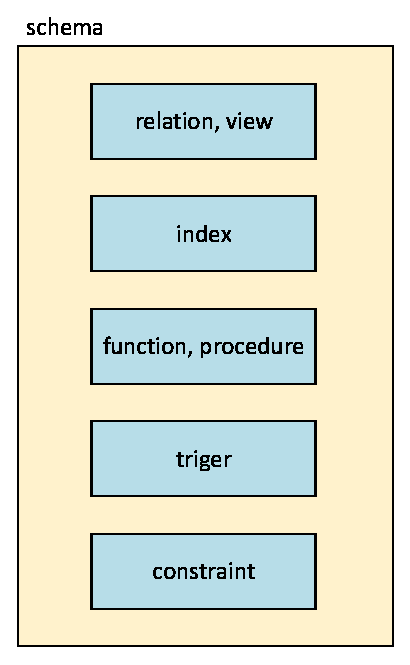
\includegraphics[width=0.4\linewidth]{handout/img/4-schema.eps}
    \caption{schema按照对象类型细分为不同名字空间}\label{fig:4-schema}
\end{figure}

在不同的数据库系统中，schema虽然是一个对象容器，但范畴有些不同。MySQL中最简单，一个库对应于一个schema，库名就是schema名。而在Oracle中，每个用户对应于一个schema，用户名就是schema名。PostgreSQL中，一个库可以创建多个schema，缺省schema为public。SQL server 2005之后，允许一个库有多个schema。从设计初衷来看，多schema主要是为了管理方便，包括权限、逻辑组织等。

MySQL中，一个库对应于一个目录，该库的所有对象（如表、视图、函数、索引等）都存储在该目录下，库的元信息放在系统的数据字典中。PostgreSQL中，一个库的所有文件、索引都放在该库名对应的OID目录下，可以通过库名找到对应的OID，这种设计是为了防止修改库名再去调整目录，PostgreSQL的schema元信息也放在系统数据字典中。

\section{Catalog}





 % 4
\chapter{Operator}

参考\figurename\ref{fig:1-arch}，前面的章节主要介绍存储引擎，本章和下一章介绍执行引擎。SQL语句大体按照如下过程执行：将SQL语句翻译为关系表达式，然后经过逻辑优化阶段，对关系表达式做等价变换。物理优化阶段，根据数据库实例的统计特征选择合适的关系算子实现算法，最后得到执行计划。

\begin{figure}[H]
    \centering
    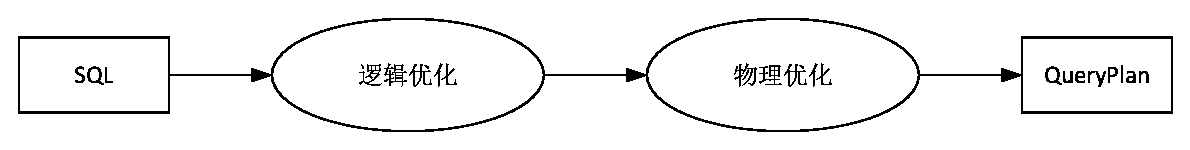
\includegraphics[width=\linewidth]{handout/img/5-plan.eps}
    \caption{SQL语句执行过程}\label{fig:5-plan}
\end{figure}

本章主要介绍如何实现表的交、并、连接、乘积等操作，这些操作会被使用在下一章的SQL解析中。一个关系模型算子可能有多种实现方式，需要关注是算子实现的性能、内存开销，同时本章还将讨论如何将算子连接以实现算子表达式。

\section{关系操作}

在讨论关系模型的算子具体实现之前，本节先回顾关系模型及其主要操作，介绍bag模型，最后讨论算法评估指标与参数。

\subsection{关系代数}

关系数据库的数据模型是\emph{关系}，数据模型是一个用于描述数据组织的抽象概念，它并非是数据库中具体实现的数据结构，而是是一个高层次的逻辑概念。一般将数据库中实现的的数据结构称为\emph{物理模型}，而称数据模型为\emph{概念模型}。数据模型的准确抽象是一类数据库成熟的标志。

在数据模型之上，数据库会定义各种操作。操作即函数，函数的参数是数据模型，后文将操作又称为算子。算子组合为算子表达式，以SQL为例，查询语句最终会被映射成一个算子表达式的实现。最后，应用采用数据模型来描述，仍然存在一些特性未能完全反应设计者的需求，比如数据完整性等，数据库需要提供一些特定的约束手段，如触发器等。

简单地说，关系就是一张二维的表，横向是行，纵向是列。横向称为tuple或者记录，纵向称为属性。每个属性都有名字，关系的属性构成一个集合，称为schema。通常一个关系的schema是固定的，属性集合是不变的，但schema与属性的排列顺序无关。逻辑上，关系的tuple如何排列也是无关的。

所谓\emph{关系代数}是指关系的操作结果仍然是关系，这样关系及其运算就构成了一个封闭的代数系统。关系的操作符有：
\begin{itemize}
    \item 单目操作，即操作符后只跟一个关系：
          \begin{enumerate}
              \item $\tau(R)$，对关系$R$做排序操作
              \item $\sigma_C(R)$，对关系$R$做选择操作，选择条件是$C$
              \item $\pi_E(R)$，对关系$R$做投影操作，投影的属性列表是$E$
              \item $\gamma_C(R)$，对关系$R$做分组，分组后的tuple做聚合操作$C$
              \item $\delta(R)$，对关系$R$去重，适用于后文的bag模型
          \end{enumerate}

    \item 双目操作，即操作符后跟两个关系：
          \begin{enumerate}
              \item $R \cap S$，关系$R$和$S$做交操作
              \item $R \cup S$，关系$R$和$S$做并操作
              \item $R - S$，关系$R$和$S$做差操作
              \item $R \times S$，关系$R$和$S$做笛卡尔积操作
              \item $R \bowtie S$，关系$R$和$S$做自然连接操作
              \item $R \bowtie_C S$，关系$R$和$S$做$\theta$连接操作，条件是$C$
          \end{enumerate}
\end{itemize}

\begin{exercise}
    单目、双目，有没有三目操作？
\end{exercise}

\subsection{bag模型}

虽然关系数据库的数据模型是关系，是tuple的集合，逻辑上不应该存在相同的tuple，但商用数据库通常采用bag数据模型，即允许关系中多次出现相同的tuple。原因是bag模型的算法实现更简单方便。例如，两个关系做并操作，$R \cup S$，如果是bag模型，简单地将所有tuple收集起来即可。

基于bag模型的关系操作，比关系模型的操作多一个$\delta$去重算子，除此外两者的算子语义有所不同，后文特别用下标$_B$表示bag模型操作。

\subsubsection*{投影$\pi_B$}

设$R$是bag模型的关系，对$R$做属性列表$E$的投影$\pi_E(R)$。结果可能出现多个相同的tuple，但结果的tuple数目与$R$相同。

\subsubsection*{选择$\sigma_B$}

设$R$是bag模型的关系，对$R$做条件为$C$的选择$\sigma_C(R)$，结果可能出现多个相同的tuple。

\subsubsection*{并$\cup_B$}

设$R$和$S$是两个bag模型的关系，一个tuple在$R$中出现$n$次，在$S$中出现$m$次，则$R \cup_B S$中，该tuple出现$n+m$次。

\subsubsection*{交$\cap_B$}

设$R$和$S$是两个bag模型的关系，一个tuple在$R$中出现$n$次，在$S$中出现$m$次，则$R \cap_B S$中，该tuple出现$min(n,m)$次。

\subsubsection*{差$-_B$}

设$R$和$S$是两个bag模型的关系，一个tuple在$R$中出现$n$次，在$S$中出现$m$次，则$R -_B S$中，该tuple出现$max(0,n-m)$次，当$n \le m$时出现$0$次，当$n \ge m$时出现$n-m$次。

\subsubsection*{积$\times_B$}

设$R$和$S$是两个bag模型的关系，则$R \times_B S$中，结果可能出现多个相同的tuple，数目为为$n \times m$。

\subsubsection*{连接$\bowtie_B$}

设$R$和$S$是两个bag模型的关系，则$R \bowtie_B S$中，结果可能出现多个相同的tuple。

\begin{figure}[H]
    \centering
    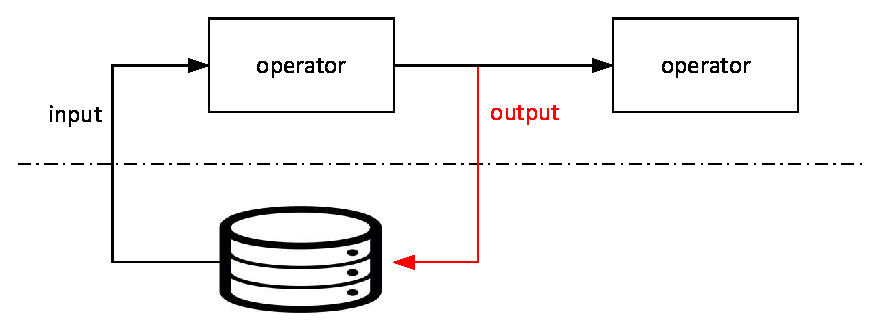
\includegraphics[width=0.8\linewidth]{handout/img/5-io.eps}
    \caption{operator连接与评估指标}\label{fig:5-io}
\end{figure}

\subsection{评估指标}

本章在比较各种操作的性能时，仍然使用磁盘IO次数这个指标。但是，\underline{本章假设输入的表都是存储在磁盘上的，而计算结果都容纳在内存中}。这里需要解释，一个算子可以有多种实现，这些实现会得到相同的结果，比较这些算子的实现时，考虑这个结果的大小不不影响对这算法性能的评估，并且有些算子会直接输出到屏幕上。算子输出结果的大小实际上与后文讨论的算子之间连接的问题有关。

另一个重要的指标是操作算法的内存使用量。通常数据库的buffer是以page为单位管理。对表操作，首先要求BufferManager调入表，所以对算法实现而言，当前能够使用的buffer总量是选择一个算子实现算法的重要依据。以$M$来表示BufferManager可用的内存，当系统轻载时$M$大致等于系统的内存总量，但是多数情况下系统总是会有多个进程，所以$M$会发生变化，有些操作系统能够实时提供这个$M$信息。

在评估算法时，还会用到一些参数，这些参数都是关系表的统计数据，如表的大小、记录的长短等。假设要操作的关系是$R$：
\begin{enumerate}
    \item $B(R)$表示存储$R$的page数目
    \item $T(R)$表示关系$R$的记录数目，$T/B$是每个page上平均存储的记录数
    \item $V(R, a)$表示$R$的属性$a$上，有多少个不同的值。如果考察$R$的部分属性列表$[a_1, a_2, ..., a_n]$，$V(R,[a_1, a_2, ..., a_n])$表示$R$关于这个属性列表不同的记录数，形式上可以表示为$\delta(\pi_{a_1, a_2, ..., a_n}(R))$
\end{enumerate}

\section{单轮算法}

本节开始讨论算子实现问题，需要实现的算子包括：投影$\pi$、选择$\sigma$、分组与统计$\gamma$、消除副本$\delta$、排序$\tau$；双目操作包括：交$\cap$、并$\cup$、差$-$、笛卡尔积$\times$、自然连接$\bowtie$、$\theta$连接$\bowtie_C$等。

在考虑算子实现方式时，需要注意几个方面的问题：
\begin{itemize}
    \item 表的大小是否能够整体调入内存。按照这个维度，可以将算子实现划分为：单轮、两轮和多轮。所谓单轮是指数据能够一次调入内存，完成处理。多轮是指数据太大，必须分成多个部分进行处理。
    \item 算子实现方式。算子可以按照page枚举，或者基于排序、基于索引。按照page枚举是最基础的形式，基于排序对应于多路归并方案，当前ssd/nvram器件逐渐流行，基于索引的方案也值得关注。
    \item 结果是否是流式输出，也就是说不必等到所有结果计算完毕就可以输出，流式输出便于与其它算子连接组合，流式输出可以分为tuple流或者page流输出。
\end{itemize}

除了上述关系算子外，还可以抽象出更多的算子，如迭代、多路归并。这些算子更为基础，它们一方面实现关系算子，同时也可以连接组合多个关系算子。

\subsection*{$\sigma_C(R)$}

在关系$R$上实现选择$\sigma_C(R)$，可以逐个枚举page，如\figurename\ref{fig:5-sigma}，然后根据条件$C$判断每个page中的记录是否满足条件。由于需要调入所有page，它的性能是$B(R)$，内存约束是$1$。

\begin{figure}[H]
    \centering
    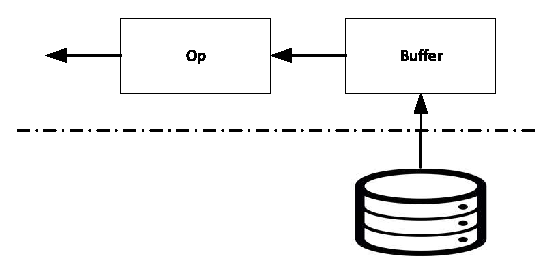
\includegraphics[width=0.5\linewidth]{handout/img/5-sigma.eps}
    \caption{选择算子实现}\label{fig:5-sigma}
\end{figure}

在bag模型或者set模型上做选择$\sigma$，输出都是bag模型，并且是tuple级别流式输出。下一章将会了解到$\sigma$下推是一个比较常用的逻辑优化方案。

\subsection*{$\pi_L(R)$}

在关系$R$上做投影$\pi_L(R)$，只需要逐个调入所有page，然后纵向截取tuple的属性即可，如\figurename\ref{fig:5-sigma}。由于需要调入所有page，它的性能是$B(R)$，内存约束是$1$。

SQL中支持扩展投影，所谓扩展投影是指$L$不仅仅是属性列表，还可以是一个判断表达式。是否是扩展投影，对方案没有影响，都必须调入所有page然后裁剪。

在set模型上做投影$\pi$，如果$L$包含主键，输出是set模型。算法支持tuple级别流式输出。$\pi$下推是一个比较常用的逻辑优化方案。

\subsection*{$\delta(R)$}

对于表空间存储的表来说，是不会有重复项的，重复项一般出现在中间结果中。去重算子$\delta(R)$挨个枚举所有page，如\figurename\ref{fig:5-delta}，同时建立一个内存索引，如果在索引中找到一条记录，则丢弃。由于需要调入所有page，它的性能是$B(R)$，不考虑索引开销的情况下内存约束是$1$。

\begin{figure}[H]
    \centering
    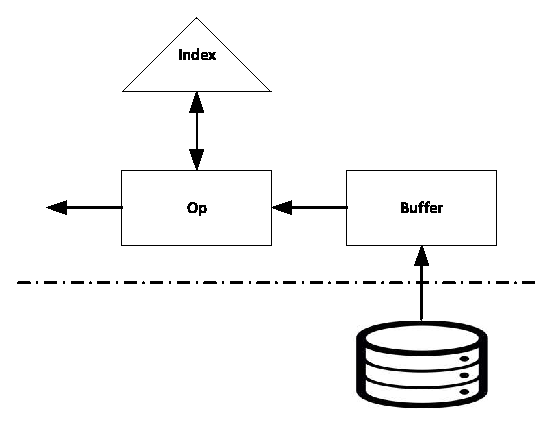
\includegraphics[width=0.5\linewidth]{handout/img/5-delta.eps}
    \caption{去重算子实现}\label{fig:5-delta}
\end{figure}

消除副本的一种开销最小的方案是采用bloom filter高概率的确定没有tuple存在。最后，去重算子支持流式输出。

\subsection*{$\tau(R)$}

单轮算法的排序方案，如\figurename\ref{fig:5-tau}，利用中间缓冲保存结果，在排完序后输出。如果中间缓冲能够兜住关系$R$，$\tau$的性能是$B(R)$，内存约束是$B(R)$。

\begin{figure}[H]
    \centering
    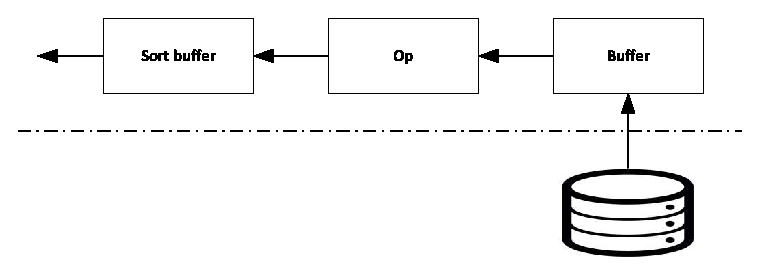
\includegraphics[width=0.8\linewidth]{handout/img/5-tau.eps}
    \caption{排序算子实现}\label{fig:5-tau}
\end{figure}

排序算子$\tau(R)$在完成前，无法输出。在后文的多路归并中，如果先保证部分有序，可以支持tuple级别流式输出。

在实现中，由于排序一般直接使用quick sort，要求连续大块内存。\figurename\ref{fig:5-tau}中的排序缓冲需要单独配置，PostgreSQL/Innodb中缺省在4MB左右。可以考虑使用内存版本的btree，这样可以直接使用buffer管理器的分页内存。此时，调入buffer的page不能swap到硬盘，同时在buffer中构建一个内存版本btree作为索引，当该表的所有页面调入完毕，内存btree索引构建完成，按照索引输出，结构上参考\figurename\ref{fig:5-delta}。

\subsection*{$\gamma_L(R)$}

在SQL语言中，GROUP BY将表中的tuple按照属性分成多个组，这些分组可以利用聚合函数做进一步处理，不加聚合函数的分组输出类似于排序$\tau(R)$，它的处理方案如\figurename\ref{fig:5-tau}。先按照分组构建一个索引，这个索引可能是键重复的，然后读入所有page，枚举tuple。当枚举完所有tuple，按照索引输出。

\begin{lstlisting}[style=verbose]
SELECT name, gender FROM employee GROUP BY gender, name
\end{lstlisting}

加了聚合函数处理的分组查询，由于输出的聚合结果，不需要保留分组后的表。由于聚合的结果一般是一个标量，所以输出的结果尺寸比较小，内存约束大致等于一个索引的大小。

下面这条语句对先按照column\_name属性分组，然后做聚合操作，最终的计算结果是一张表，表以column\_name为键，另一个属性是聚合函数计算出来的标量。

\begin{lstlisting}[style=verbose]
SELECT column_name, aggregate_function(column_name)
FROM table_name
WHERE column_name operator value
GROUP BY column_name
\end{lstlisting}

如果存在索引，并且按照索引分组做聚合，则可以利用索引直接处理，不需要调入page，性能很高。

与排序$\tau$类似，分组$\gamma$必须等待所有结果处理完毕后，才能输出。

\subsection*{$R \cup S$}

两个bag模型关系的并$R \cup S$，只需将两个关系合并即可。逻辑上需要枚举两个关系的所有page，但实际上可以做一个简单的记号即可。

\subsection*{$R \cap S$}

两个bag模型关系的交$R \cap S$，先将关系$R$逐page调入内存，建立$R$的索引并记录相同tuple出现的次数，然后丢弃掉该page。再将关系$S$逐page调入内存，比较tuple，如果一个tuple在索引中出现，则将引用计数减1，然后输出；否则丢弃。它的性能是$B(R)+B(S)$，内存约束是$1$。

\begin{figure}[H]
    \centering
    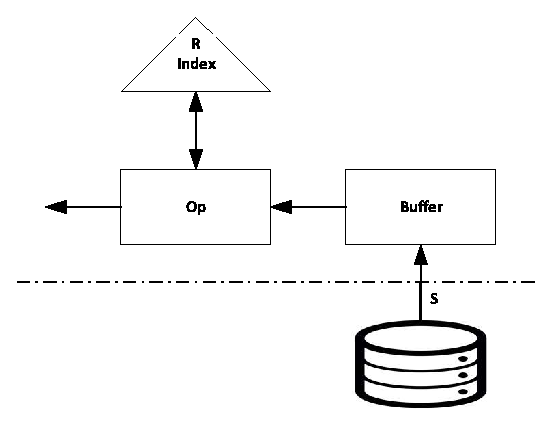
\includegraphics[width=0.6\linewidth]{handout/img/5-cap.eps}
    \caption{交算子实现}\label{fig:5-cap}
\end{figure}

以上是bag模型实现，但考虑到引入bag模型无非是为了方便实现，其实基于bag模型的交实现比set交要复杂一些。bag交与set交的实现，仅在$R$全部调入内存后，支持tuple级别流式操作。

\begin{exercise}
    设计set交方案。
\end{exercise}

\subsection*{$R - S$}

两个bag模型关系的差$R - S$，如\figurename\ref{fig:5-minus}，先将关系$R$逐page调入内存，然后建立索引记录次数，再将关系$S$逐page调入内存，比较tuple，当引用计数减到0，删除索引条目；如果$S$的tuple没有命中索引条目，直接drop掉。当$S$的所有tuple枚举完毕，按照索引输出。它的性能是$B(R)+B(S)$，内存约束是$B(R)+1$。如果存在索引，就更简单一些。

\begin{figure}[H]
    \centering
    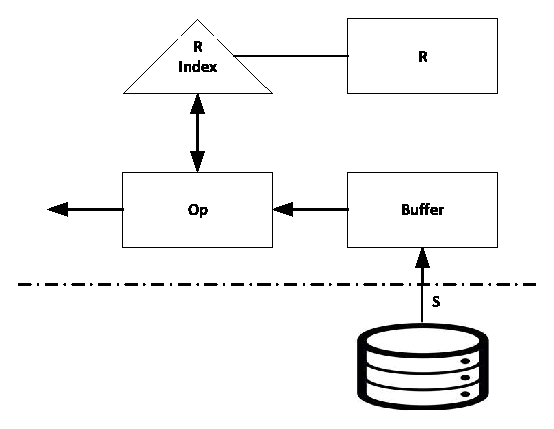
\includegraphics[width=0.6\linewidth]{handout/img/5-minus.eps}
    \caption{差算子实现}\label{fig:5-minus}
\end{figure}

差算子必须等结果计算完毕后才能输出。

\begin{exercise}
    设计set差方案。
\end{exercise}

\subsection*{$R \times S$}

两个bag模型关系的积$R \times S$，需要将$R$中的tuple与$S$中的每个tuple做合并处理，先将$S$整体调入内存，然后再逐个调入$R$的page，结构如\figurename\ref{fig:5-minus}。如果$min(B(R),B(S))+1 \le M$，性能是$B(R)+B(S)$，内存约束是$min(B(R),B(S))+1$。乘积可以直接tuple输出。

\subsection*{$R \bowtie S$}

两个bag模型关系的积$R \bowtie S$，需要将$R$和$S$中的tuple按照某个属性做连接处理。先将$S$整体调入内存，然后再逐个调入$R$的page，结构如\figurename\ref{fig:5-minus}。$min(B(R),B(S))+1 \le M$，性能是$B(R)+B(S)$，内存约束是$min(B(R),B(S))+1$。连接可以直接tuple输出。

总结一下，单目、双目算子在单轮算法的性能如\tablename\ref{tab:5-single}。
\begin{table}[H]
    \centering
    \caption{单轮算法性能表}\label{tab:5-single}
    \begin{tabular}{lccc}
        \toprule
        算子 & 内存约束 & 磁盘IO & 流输出 \\
        \midrule
        $\sigma, \pi, \delta$ & $1$ & $B$ & \checkmark \\
        $\gamma, \tau$        & $B < M$ & $B$ & \ding{55} \\
        $\cup$                & $1$ & $B(R) + B(S)$ & \checkmark \\
        $\cap$                & $1$ & $B(R) + B(S)$ & \checkmark \\
        $-$                   & $B(R) < M$ & $B(R) + B(S)$ & \ding{55} \\
        $\times, \bowtie, \bowtie_C$ & $min(B(R),B(S))) < M$ & $B(R) + B(S)$ & \checkmark \\
        \bottomrule
    \end{tabular}
\end{table}

在\tablename\ref{tab:5-single}中，$\sigma, \pi, \delta, \cup$这几个算子的内存约束仅为1，又支持流输出，后续将不再关注这几个算子的实现，这些算子均采用单轮算法。后面主要关注$\gamma, \tau, -, \times, \bowtie, \bowtie_C$这几个算子。

\section{nested-loop}

嵌套循环主要用于实现$\times, \bowtie, \bowtie_C$这几个算子。

\subsection*{$R \times S$}

假设$min(B(R),B(S)) > M$，无法使用单轮算法。嵌套循环比较直观，尽可能的调入$R$或$S$，设调入部分是$S_1$，然后逐page调入$R$，将$R$的tuple与$S_1$的tuple组合；然后再尽可能调入$S_2$，重复上述动作。

\begin{figure}[H]
    \centering
    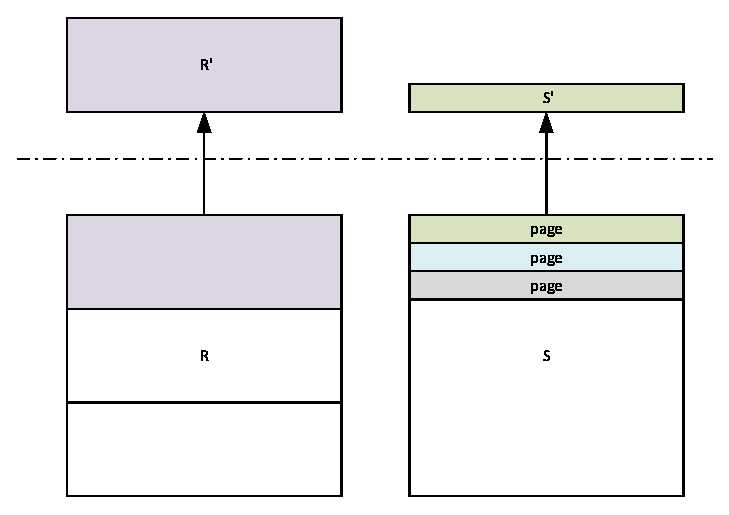
\includegraphics[width=0.8\linewidth]{handout/img/5-nested.eps}
    \caption{积算子nested-loop实现}\label{fig:5-nested}
\end{figure}

如\figurename\ref{fig:5-nested}所示，nested-loop算法先尽可能将$R$调入内存，然后逐个将$S$的页面调入内存，与$R$的每个tuple组合。

在\figurename\ref{fig:5-nested}中，$R$会调入一轮，$S$会调入$B(S)B(R)/M$轮，支持tuple流输出。对于$\times$算子，nested-loop是一个重要实现，后面介绍的排序归并方案中，排序无助于提升性能。

\subsection*{$R \bowtie S$}

方案与$R \times S$相同。

\section{两轮算法}

单轮算法要求关系能被整体调入内存，如果关系的尺寸很大，难以做到。两轮、多轮算法首先将关系排序，持久化后再做进一步处理，内存约束可以小于$M$，多路归并是一类通用的算子实现方案。在分布式系统中，多路归并与mapreduce、spark这样的任务调度框架相结合，用途很广。

\subsection*{$\tau$}

根据\tablename\ref{tab:5-single}，$B > M$无法使用单轮算法。两轮多路归并排序算法$\tau$如图\ref{fig:5-sort}所示，算法分为两个轮：
\begin{enumerate}
    \item 将$R$均分为$M$个分片，每个分片大小为$B(R)/M$。每次读入一个分片，然后排序，将排序后分片写入磁盘；
    \item 从$M$个分片读1个page，在每个分片上设置一个指针。分片已经排序，指针按照顺序枚举所有记录。merge算子从$M$个指针指向的记录中选取最小的记录输出。
\end{enumerate}

\begin{figure}[H]
    \centering
    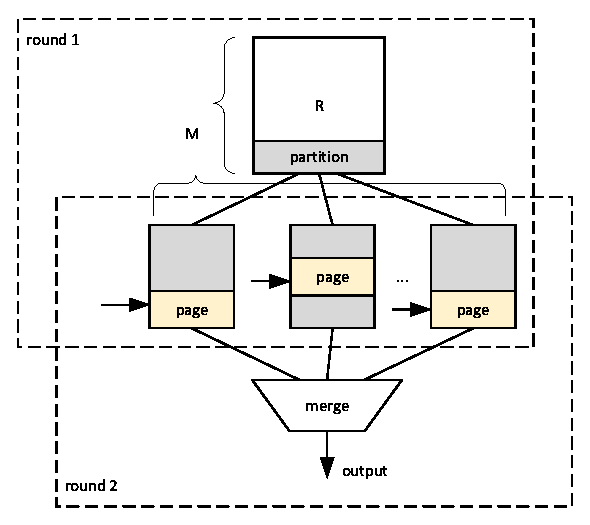
\includegraphics[width=0.8\linewidth]{handout/img/5-sort.eps}
    \caption{排序归并算法$\tau$实现}\label{fig:5-sort}
\end{figure}

两轮多路归并排序，在第2轮，不考虑输出buffer，至多能容纳$M$个块，内存约束是$M < B(R) < M*M$。一般情况下，两轮多路归并排序可以处理大多数关系，但是有些表尺寸太大，会超过这个内存约束，此时会用到某个的多轮多路归并算法处理。

两轮多路归并排序在第1轮读入$B$个块，写出$B$个块，第2轮读入$B$个块，所以磁盘IO开销是$3B$。得益于分片是排序的，方案在第2轮支持tuple流输出。

\subsection*{$\gamma$}

分组后如果使用聚合函数，在第2轮归并后应用聚合函数。

\begin{exercise}
    设计$\gamma$算子的两轮多轮归并算法。
\end{exercise}

\subsection*{$-$}

差算子在$B(R) < M$时，无法使用单轮算法。两轮多路归并的差算子实现如\figurename\ref{fig:5-minus2}所示，先将$R, S$分为$M$个分片，每个分片大小为$(B(R)+B(S))/M$，对每个分片排序后回写到硬盘。在第2轮，调入$R,S$的$M$个分片，从$R, S$的分片中选取最小的记录。bag模型下，如果两条记录匹配，则drop掉，否则输出$R$的最小记录。

\begin{figure}[H]
    \centering
    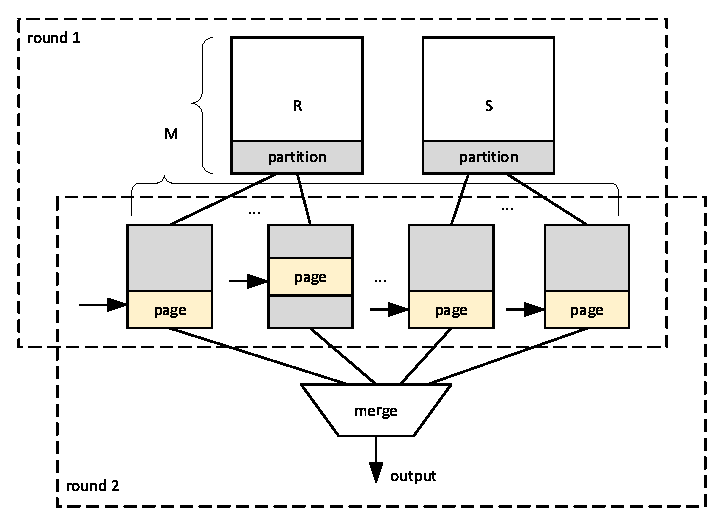
\includegraphics[width=\linewidth]{handout/img/5-minus2.eps}
    \caption{差算子两轮多路归并实现}\label{fig:5-minus2}
\end{figure}

\figurename\ref{fig:5-minus2}的方案中，$R,S$被调入两轮，开销是$3(B(R) + B(S))$。在第2轮开始后，支持tuple流输出，内存约束是$(B(R)+B(S) )< M^2$。

两轮多路归并差算子的方案可以进一步优化，先调入$S$，同时构造一个索引。然后对$R$做多路归并，每次从$R$的分片中选取最小的记录，与索引中的记录匹配。如果匹配，则drop掉，否则输出$R$的最小记录。

\begin{figure}[H]
    \centering
    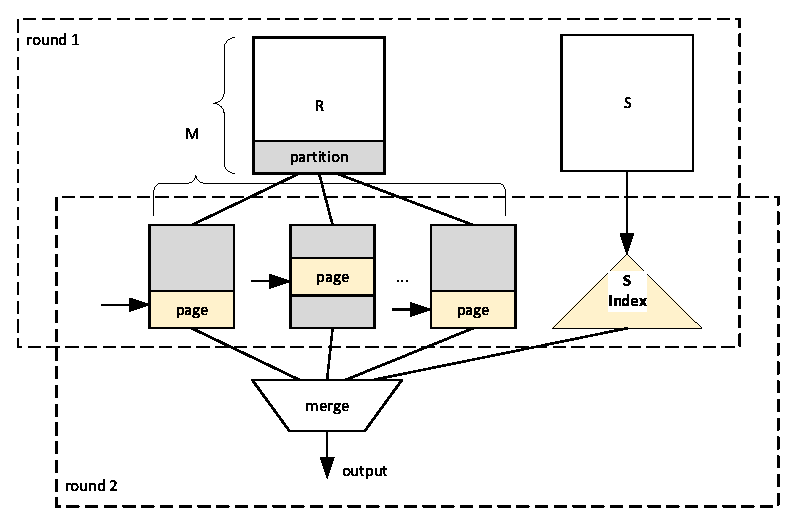
\includegraphics[width=\linewidth]{handout/img/5-minus3.eps}
    \caption{差算子两轮多路归并优化实现}\label{fig:5-minus3}
\end{figure}

\figurename\ref{fig:5-minus3}的方案中，$R$被调入两轮，$S$被调入一轮，开销是$3B(R) + B(S)$。在第2轮开始后，支持tuple流输出，内存约束是$B(R) < M^2$。

\begin{exercise}
    在\figurename\ref{fig:5-minus3}方案下，讨论bag和set模型的实现差异。
\end{exercise}

\subsection*{$\bowtie$}

\subsubsection*{基本方案}

$\bowtie$基本方案如\figurename\ref{fig:5-minus2}所示，先将$R, S$分为$M$个分片，每个分片大小为$(B(R)+B(S))/M$，对每个分片排序后回写到硬盘。在第2轮，调入$R,S$的$M$个分片，从$R, S$的分片中选取最小的记录。如果两条记录匹配，则输出，否则drop掉。

这个方案有一个潜在的问题：假设$S$的一条记录与$R$分片中的记录可以连接，然后移动$R$分片上的指针，当指针耗尽了分片上该page的所有记录，就应该调入下一个页面。此时，假设$S$的另一个分片上的记录也可以连接，但这个分片上的记录已经错失了机会。

这个问题在bag模型下尤为突出，set模型会好些，但仍然会出问题，问题的本质是$R,S$可连接的记录延展到多个page，如\figurename\ref{fig:5-join}所示。

\begin{figure}[H]
    \centering
    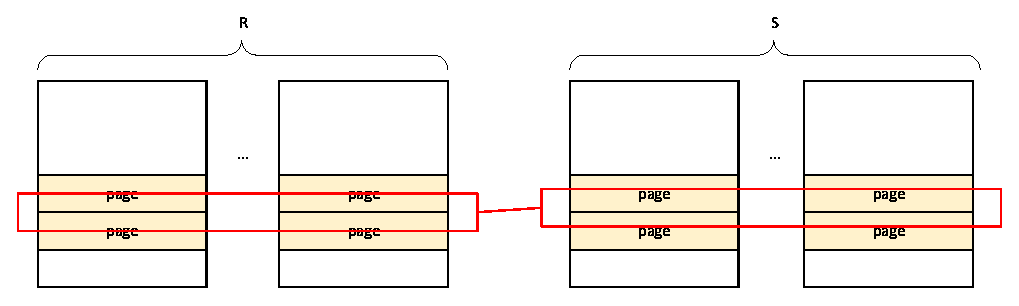
\includegraphics[width=\linewidth]{handout/img/5-join.eps}
    \caption{连接算子的潜在问题}\label{fig:5-join}
\end{figure}

\subsubsection*{改进方案}

一个改进方案是三轮，如\figurename\ref{fig:5-join2}所示。
\begin{enumerate}
    \item 用两轮多路归并方案分别对$R,S$排序，排序后回写磁盘。
    \item 采用两路归并处理$R\bowtie S$，这样就尽可能的在$M$内存大小容纳$R,S$的可连接记录。
\end{enumerate}

\begin{figure}[H]
    \centering
    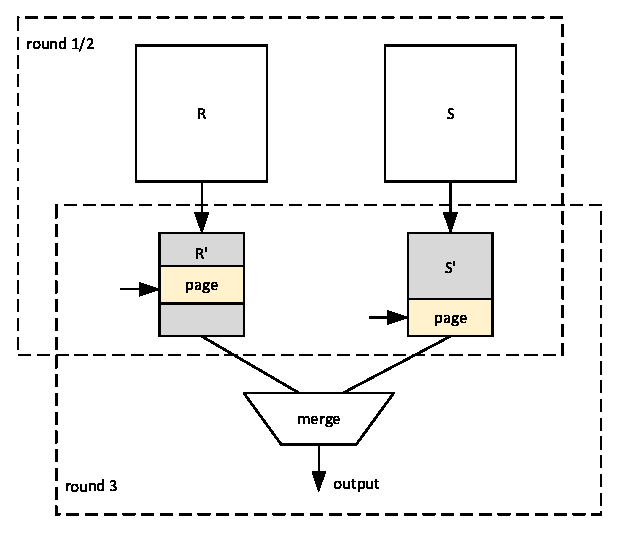
\includegraphics[width=0.8\linewidth]{handout/img/5-join2.eps}
    \caption{连接算子改进方案}\label{fig:5-join2}
\end{figure}

这个改进方案跑了三轮，io开销是$3(B(R) + B(S))$，并且仍然不能完全杜绝连接算子的潜在问题。

\subsubsection*{进一步改进}

对$R\bowtie S$的进一步改进，如\figurename\ref{fig:5-join3}所示。
\begin{enumerate}
    \item 对$R,S$分片，分片大小为$(B(R)+B(S))/M$。将分片调入内存，对$R,S$分别构建索引，索引指向排序后的分片。
    \item 按照$R,S$的索引，做zig-zag扫描，进行匹配，匹配成功调入$R,S$排序好的分片，进行连接。
    \item 如果$R,S$的可连接记录数在$M$内存中兜不住，产生内存溢出则使用前述的nested-loop方案处理。
\end{enumerate}

\begin{figure}[H]
    \centering
    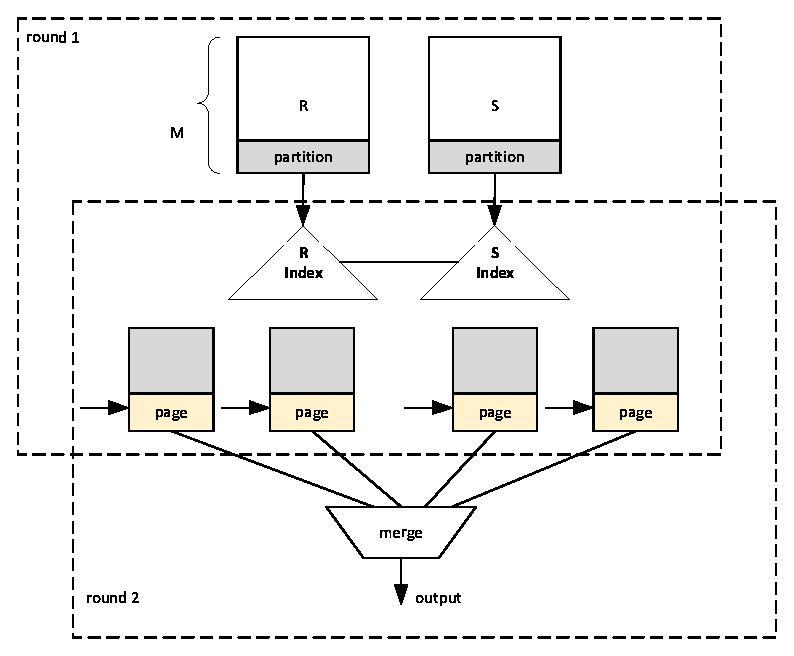
\includegraphics[width=\linewidth]{handout/img/5-join3.eps}
    \caption{连接算子进一步改进}\label{fig:5-join3}
\end{figure}

\figurename\ref{fig:5-join3}的性能基本是$3(B(R) + B(S))$，内存约束是$(B(R)+B(S) )< M^2$，在第2轮可以tuple流输出。

总结一下两类多路归并算法，如\tablename\ref{tab:5-two}所示。

\begin{table}[H]
    \centering
    \caption{两轮算法性能表}\label{tab:5-two}
    \begin{tabular}{lccc}
        \toprule
        算子 & 内存约束 & 磁盘IO & 流输出 \\
        \midrule
        $\tau, \gamma$ & $M < B(R) < M^2$ & $3B$ & \checkmark \\
        $-$   & $M < B(R) < M^2$ & $3B(R) + B(S)$ & \checkmark \\
        $\bowtie$ & $M < (B(R) + B(S)) < M^2$ & $3(B(R) + B(S))$ & \checkmark \\
    \bottomrule
    \end{tabular}
\end{table}

\subsection{多轮算法}

递归的多轮排序$\tau$算法如下：

\textbf{基础}：如果$R$能够整体调入$M$，采用单轮排序算法处理$R$，然后写盘。

\textbf{递推}：如果$R$不能整体调入$M$，将$R$拆分成$M$个子表$R_1, R_2, ..., R_M$。然后递归地对每个$R_i$做排序，最后对$M$个子表做多路归并。

其余多轮算法可以模仿这个排序算法处理，这个多轮算法将单轮、双轮、多轮集成到一个框架，简化了算法选择。

\section{基于索引的算法}

索引相较于数据，尺寸要小得多，可以利用索引来快速定位需要加载的page。采用索引来实现算法的问题是，当沿着索引扫描，可能会遇到一个page被反复加载的问题。没法完全规避这个问题，但是考虑到缓冲层的存在，page被反复加载的概率比较小。

在前述递归多路归并基础上，如果表上有索引，要优先采用索引来处理。现在重新考虑如下算子的实现方案：$\sigma, \delta, \tau, \gamma, \cap, -, \bowtie$。

\subsection*{$\sigma$}

在索引上根据$\sigma_{a=v}(R)$查找，根据条目调入相应的page。如果索引是聚集的，平均指标为$B(R)/V(R,a)$，其中$V(R,a)$是$R.a$不同属性数量，实际的指标可能要比这个值高一些。

如果索引是非聚集的，索引的tuple散布在各个page上，并且$R.a=v$条件可能会对应于多个tuple，$T(R)/V(R,a)$是这个条件平均需要访问的page数目，性能大约是$min(B(R), T(R)/V(R,a))$。

举例而言，假设$B(R)=1000$，$T(R)=20000$，即$R$有20000个tuple存放在1000个page上。考虑$R$的$a$属性上的$\sigma_{a=v}(R)$操作：
\begin{enumerate}
    \item 如果$R$聚集，不使用索引，磁盘IO为$B(R)$
    \item 如果$R$非聚集，不使用索引，磁盘IO为$T(R)$
    \item 假设$V(R,a)=100$，聚集索引，$\sigma_{a=v}(R)$操作的平均磁盘IO为$B(R)/V(R,a)=10$，再加上索引的IO数量
    \item 假设$V(R,a)=10$，非聚集索引，$\sigma_{a=v}(R)$操作的平均磁盘IO为$T(R)/V(R,a)=2000$，再加上索引的IO数量
    \item 假设$V(R,a)=20000$，$a$是$R$的主键，$\sigma_{a=v}(R)$操作的平均磁盘IO为1，再加上索引的IO数量
\end{enumerate}

上述的选择是一种简单的相等$\sigma_{a=v}(R)$操作，如果查询的条件更复杂，比如$\sigma_{a \ge 10\ \sf{AND}\ a \le 20}(R)$，可以在btree上处理。同时，对形如$\sigma_{a=v\ \sf{AND}\ C'}(R)$这样的复杂查询，可以先花少量磁盘IO处理$R.a=v$，然后再处理$C'$条件。

\subsection*{$\bowtie$}

两个表做自然连接$R(X,Y) \bowtie S(Y,Z)$，如果$R,S$上都有索引，可以采用\figurename\ref{fig:5-zigzag}的zig-zag扫描方案。沿着索引$R.Y$和$S.Y$移动指针，找到匹配的tuple，做自然连接。整个动作过程就象啮合的两个齿轮，称为zig-zag扫描。

\begin{figure}[H]
    \centering
    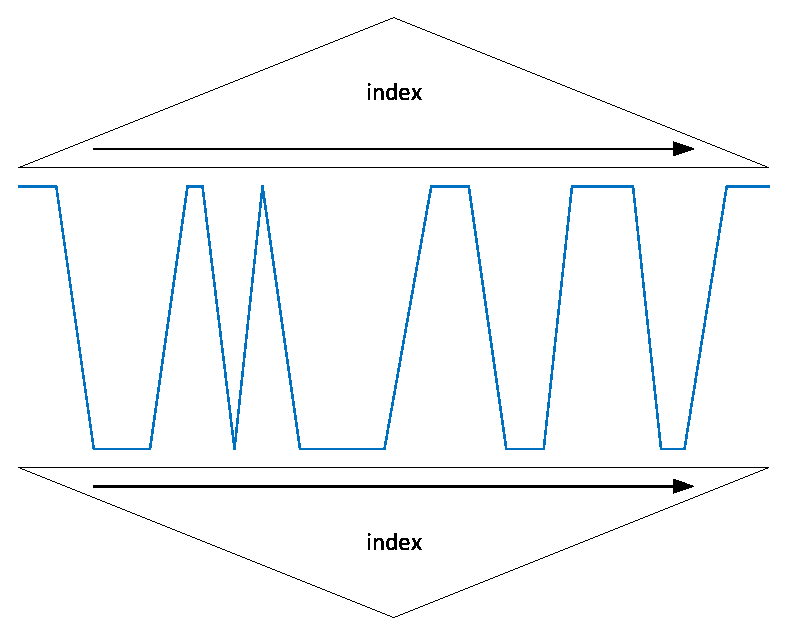
\includegraphics[width=0.5\linewidth]{handout/img/5-zigzag.eps}
    \caption{zig-zag扫描}\label{fig:5-zigzag}
\end{figure}

如果$R$是聚集的，枚举$R$需要$B(R)$的磁盘IO；如果如果$R$是非聚集的，枚举$R$需要$T(R)$的磁盘IO。

每个$R$的tuple平均需要读取$T(S)/V(S,Y)$个$S$上的tuple。如果$Y$是$S$的非聚集索引，则平均磁盘IO开销为$T(S)/V(S,Y)$。如果$Y$是$S$的聚集索引，平均磁盘IO开销为$max(1,B(S)/V(S,Y))$。


\section{算子连接}

SQL语句被解析成算子表达式，经过优化后要得到一个执行计划，执行计划中各个算子的实现算法需要彼此连接起来，关系和中间计算结果要流经各个算法，最终得到SQL查询结果。

本节讨论如何将各个算子连接起来，数据如何流经各个算子。一般来说，算子的组合主要有两种方式：一是tuple流，二是\emph{物化}，所谓物化是指中间计算结果以关系的形式被完整保存在磁盘上。在分布式系统中，算子连接还涉及mapreduce、spark这样的调度框架。

\begin{figure}[H]
    \centering
    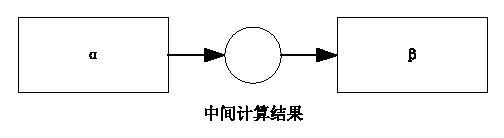
\includegraphics[width=0.7\linewidth]{handout/img/5-connect.eps}
    \caption{两个算子连接}\label{fig:5-connect}
\end{figure}

用函数的形式表示算子，假设两个算子$\alpha, \beta$，在算子表达式表示为$\alpha\beta(R)$。如果$\beta(R)$输出tuple流，并且$\alpha$接受tuple流，就可以将两个算法用tuple串联起来。

\subsection{迭代器}

关系算子的实现往往依赖于一个更基础的算子——迭代。迭代器可以看成一个对象，它暴露一个next()函数，该函数返回一条记录。基础的迭代器包括：
\begin{itemize}
    \item tablescan，按照page迭代
    \item indexscan，按照索引迭代
    \item pagescan，枚举一个page内部的tuple
\end{itemize}
 % 5
\chapter{Query}

上一章主要讨论关系算子的实现问题，本章介绍SQL语句如何被翻译成算子表达式，算子表达式如何优化等问题。按照前一章所述，整个过程分为两步：生成逻辑执行计划，得到物理执行计划。详细的过程包括：
\begin{enumerate}
    \item 生成CST语法树
    \item CST上的预处理
    \item 生成算子表达式（或者抽象语法树AST）
    \item 优化逻辑执行计划
    \item 优化物理执行计划
\end{enumerate}

在SQL翻译阶段，主要利用编译原理的技术对SQL语句做词法、语法分析，得到一棵语法树，然后在语法树上做类型检查、视展开等预处理。这棵语法树需要被翻译成为算子表达式，算子表达式表现为AST抽象语法树。接下来需要变换算子表达式，目的是使算子表达式更容易计算，然后生成逻辑执行计划。最后选择算子实现算法，得到物理执行计划。逻辑执行计划与物理执行计划的优化方式有两种：一种是采用直观的规则，另一种是根据算法的性能做动态规划。

\begin{figure}[H]
    \centering
    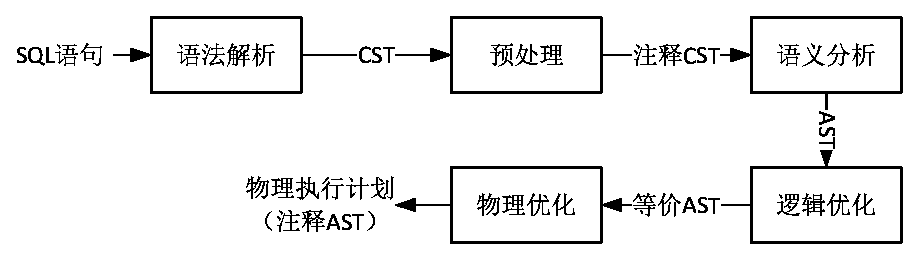
\includegraphics[width=\linewidth]{handout/img/6-process.eps}
    \caption{查询处理过程}\label{fig:6-process}
\end{figure}

\section{SQL语法解析}

在编译原理中，通常用正则表达式RE来描述词法，通过有限自动机FA来识别词法，有限自动机能识别的语言等价于正则表达式描述的语言。有限自动机输出为一个token流，在此基础上做语法解析。

当前绝大多数计算机语言使用上下文无关文法CFG来描述，使用堆栈下推自动机PDA来识别语法，二者也是等价的。CFG文法定义可能存在歧义，不能保证语法树的唯一性，并且理论上不存在判定CFG是否歧义的算法。另一方面，通用下推自动机PDA存在需要$O(n^3)$的复杂度来识别语法，这个复杂度太高了，人们追求的是在$O(n)$线性复杂度内识别语言。所幸的是，存在LL/LR这样的算法能够在线性复杂度识别某些CFG文法的结构，并且是保证无歧义。

\subsection{SQL子集文法}\label{sec:query-sql}

SQL语句按照语法规则被解析为一颗具体语法树CST。语法树的叶子节点称为\emph{终止符}，包括关键字、标识符、符号等，语法树的内部节点称为\emph{非终止符}。具体来说，终止符包括：1)~关键字，如\texttt{SELECT}、\texttt{WHERE}、\texttt{FROM}等；2)~对应于表名或者属性名的标识符；3)~表达式的各种符号，如\texttt{(}、\texttt{)}、\texttt{=}等。

这里以一个SQL子集文法作为示例，展示如何描述和识别SQL语言。这个子集没有包括\texttt{GROUP BY}、\texttt{ORDER BY}等产生式，完整的SQL语法定义可以参考\cite{SQLSynta19:online}。

这个SQL子集的语法产生式如下：

\begin{lstlisting}[style=verbose]
<Query> ::= SELECT <SelList> FROM <FromList> WHERE <Condition>
<SelList> ::= <Attribute>, <SelList>
<SelList> ::= <Attribute>
<FromList> ::= <Relation>, <FromList>
<FromList> ::= <Relation>
<Condition> ::= <Condition> AND <Condition>
<Condition> ::= <Attribute> IN ( <Query> )
<Condition> ::= <Attribute> = <Attribute>
<Condition> ::= <Attribute> LIKE <Pattern>
\end{lstlisting}

在SQL语法子集中，\texttt{<Query>}位于生成式左部，是一个非终止符，并且是整个语法生成式的根。\texttt{<Attribute>}、\texttt{<Relation>}、\texttt{<Pattern>}三个是终止符，词法分析器是无法判定这样的token类型的，必须在语义分析阶段由上下文来解释。\texttt{<Relation>}是指关系名称，\texttt{<Attribute>}指关系包含的属性名，\texttt{<Pattern>}指模式匹配的字符串。

按照语法规则，采用top-down或者bottom-up方法，将SQL语句解析为一颗具体语法树CST后，语法分析阶段就结束了，后面是语义分析阶段。

\begin{example}\label{exp:6-cst}
    假设有两张表定义如下：
\begin{lstlisting}[style=verbose]
    StarsIn(movieTitle, movieYear, starName)
    MovieStar(name, address, gender, birthdate)
\end{lstlisting}
在这两张表上执行查询语句：
\begin{lstlisting}[style=verbose]
    SELECT movieTitle
    FROM StarsIn
    WHERE starName IN (
        SELECT name
        FROM MovieStar
        WHERE birthdate LIKE '%1960'
    );
\end{lstlisting}
词法分析器首先扫描整个语句，识别token。\texttt{SELECT}被识别为一个关键字，token类型假设为1，然后movieTitle被识别成为一个关系属性，假设token类型为2。如此，当词法分析器识别一个token，然后输出token流。

语法分析器拿到token流后，根据LL或者LR语法解析程序，将token流装配成一棵具体语法树\figurename\ref{fig:6-cst}。注意这个查询语句是嵌套的，内层\texttt{SELECT}语句查询出一张表，然后使用\texttt{starName IN}表示相等。
\end{example}

\begin{figure}[H]
    \centering
    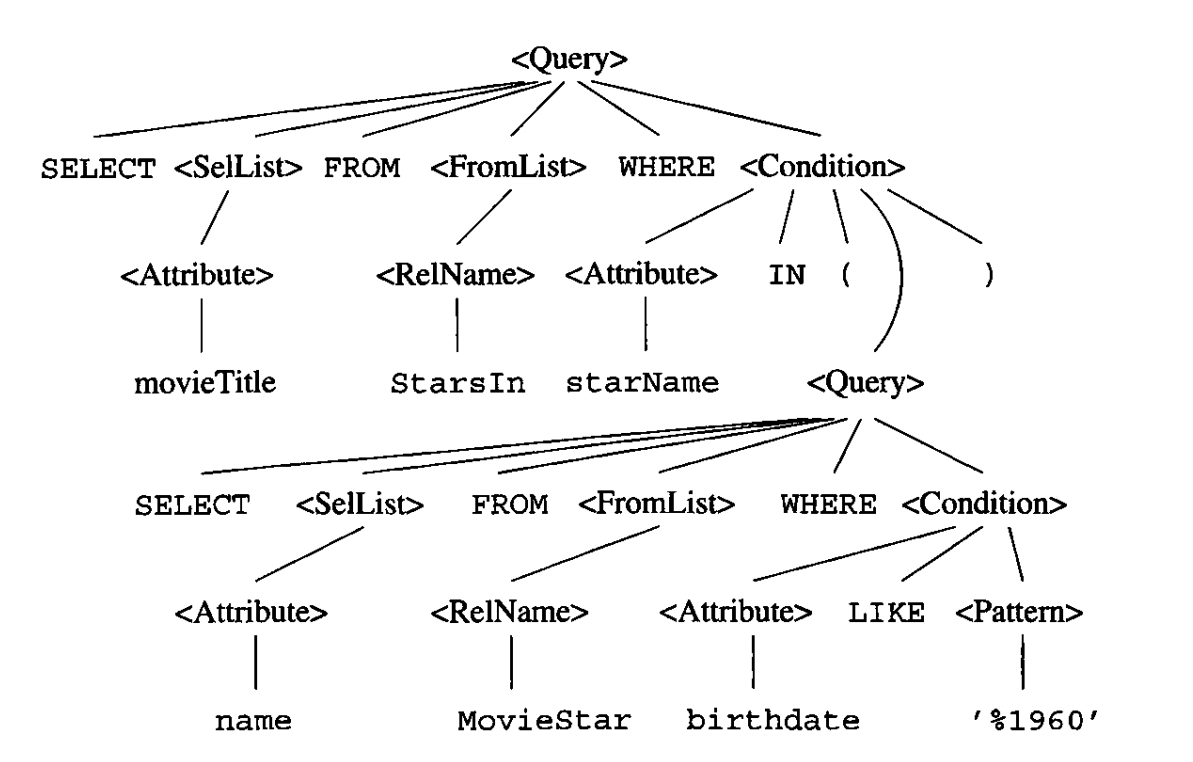
\includegraphics[width=\linewidth]{handout/img/6-cst.png}
    \caption{具体语法解析树CST}\label{fig:6-cst}
\end{figure}

\begin{example}\label{exp:6-cst2}
    \examplename\ref{exp:6-cst}采用嵌套方式查询，另一种方式采用多个条件的方式来查询：
\begin{lstlisting}[style=verbose]
    SELECT movieTitle
    FROM StarsIn, MovieStar
    WHERE starName = name AND birthdate LIKE '%1960';
\end{lstlisting}

    这个SQL语言被翻译成两个条件的组合，如\figurename\ref{fig:6-cst2}。
\end{example}

\begin{figure}[H]
    \centering
    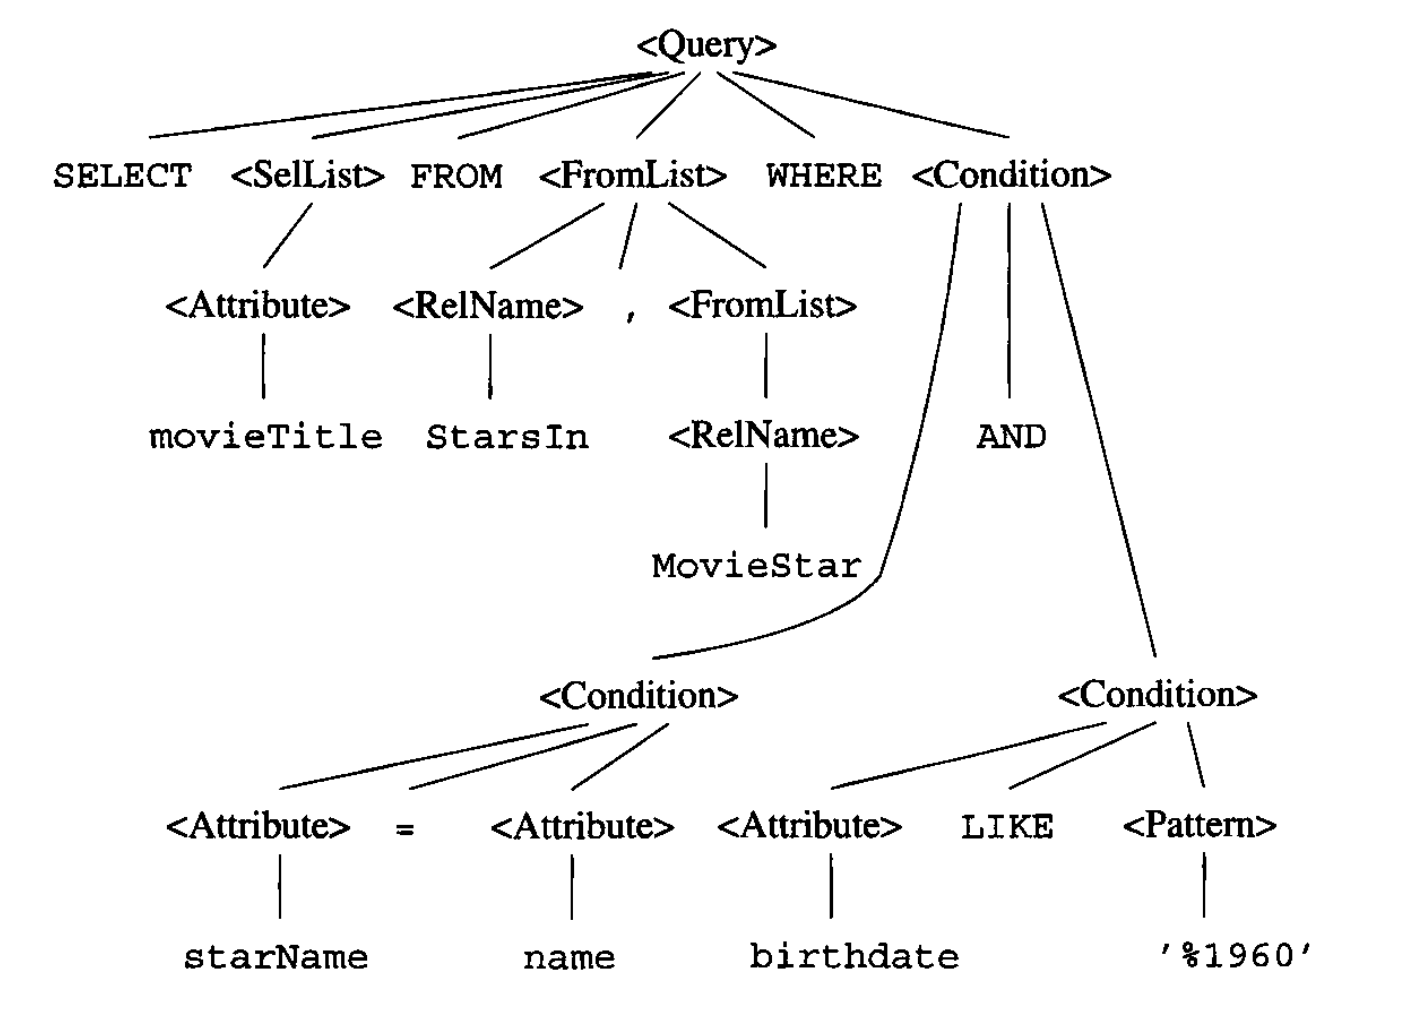
\includegraphics[width=\linewidth]{handout/img/6-cst2.png}
    \caption{具体语法解析树CST}\label{fig:6-cst2}
\end{figure}

\subsection{类型检查}

得到语法解析树CST后，接下来是语义分析，站在编译原理的角度，本章大部分的内容都是语义分析与优化。

一般来说，语义分析的第一步要检查变量的类型。与c语言不同，SQL语言没有变量声明，所以\examplename\ref{exp:6-cst}中\texttt{MovieStar}先被识别为某种类型的token，然后根据它在树中的位置确定为关系，去schema中查找是否有这样的关系。再去确定\texttt{name}是否出现在这个关系的属性中，检查条件判断中\texttt{birthdate}是否有这样的属性。

内部嵌套的这个\texttt{SELECT}语句输出为一个关系，这个关系的属性只有\text{name}字段。语句\texttt{WHERE starName IN}表示一个选择条件。

总结下来，类型检查的主要工作包括：
\begin{itemize}
    \item 检查from-list的关系变量是否有效
    \item 检查select-list或者condition的属性是否有效
    \item 检查类型，检查属性使用的类型是否满足各种计算的要求
\end{itemize}

类型检查围绕AST语法树做深度遍历，在树上做标记。一般的计算过程是先根据\texttt{<FromList>}生成式右部的\texttt{<Relation>}确定关系，然后再确定\texttt{<SelList>}和\texttt{<Condition>}中的属性，最后在\texttt{<Query>}节点上标注输出关系的属性集合。

\subsection{view展开}

在CST语法树上做类型检查时，还会碰到一些token为虚拟视view的情况。所谓视实际上是一条查询语句，SQL可以创建一个视，一个视并不一定意味着有底层存储的关系与之对应。如\figurename\ref{fig:6-view}，在语义解析时view需要展开成一段查询语句，效果上类似于嵌套查询。

\begin{figure}[H]
    \centering
    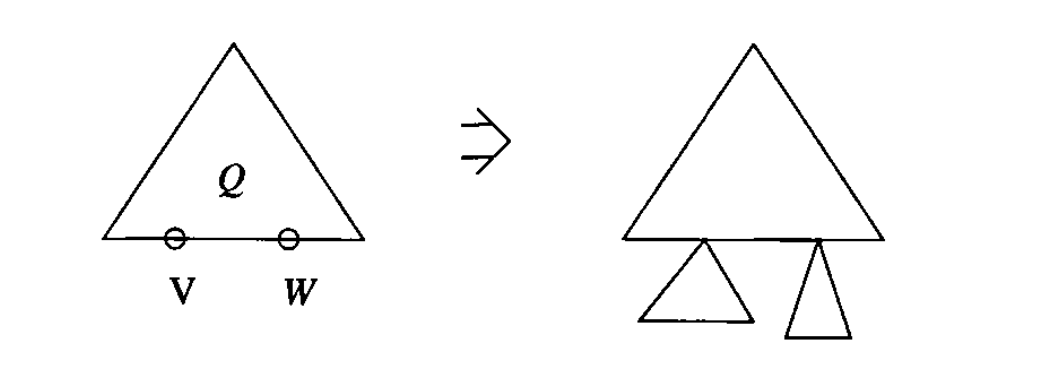
\includegraphics[width=0.5\linewidth]{handout/img/6-view.png}
    \caption{视的替换展开}\label{fig:6-view}
\end{figure}

view在某些数据库实现中会持久化为一张表，通过创建一些常用的视可以加快数据库查询过程，因为视可以看成是物化的中间结果。另外，教材中将类型检查与view展开都称为预处理是有道理的，它暗指这两个动作在一次CST遍历中处理。

\begin{example}\label{exp:6-view}
    利用下面的语句创建一个名为ParamountMovies的视：
\begin{lstlisting}[style=verbose]
    CREATE VIEW ParamountMovies AS
        SELECT title, year
        FROM Movies
        WHERE studioName = 'Paramount';
\end{lstlisting}

这个视的CST语法树表示为\figurename\ref{fig:6-view1}。假设有一条查询语句为：
\begin{lstlisting}[style=verbose]
    SELECT title
    FROM ParamountMovies
    WHERE year = 1979;
\end{lstlisting}

查询语句做语法解析后得到\figurename\ref{fig:6-view2}，对查询CST做深度遍历，如\figurename\ref{fig:6-view3}。遍历中，检查类型同时做view展开，最后得到\figurename\ref{fig:6-view4}。
\end{example}

\begin{figure}[H]
    \centering
    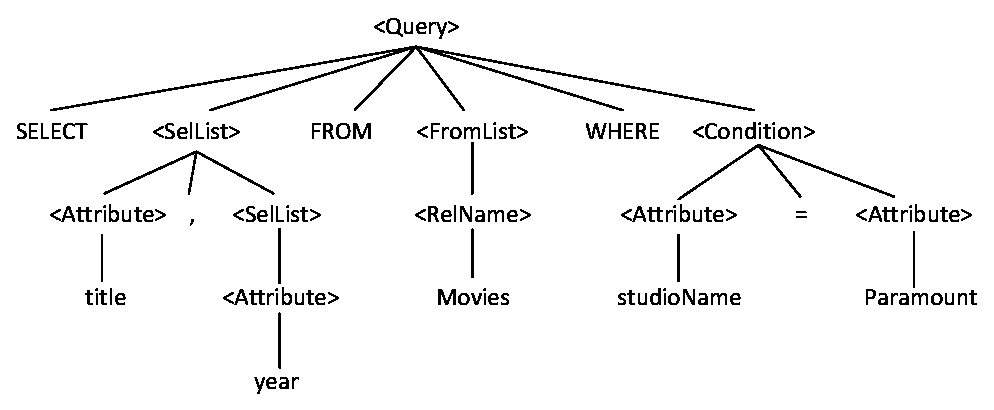
\includegraphics[width=\linewidth]{handout/img/6-view1.eps}
    \caption{view的CST}\label{fig:6-view1}
\end{figure}
\begin{figure}[H]
    \centering
    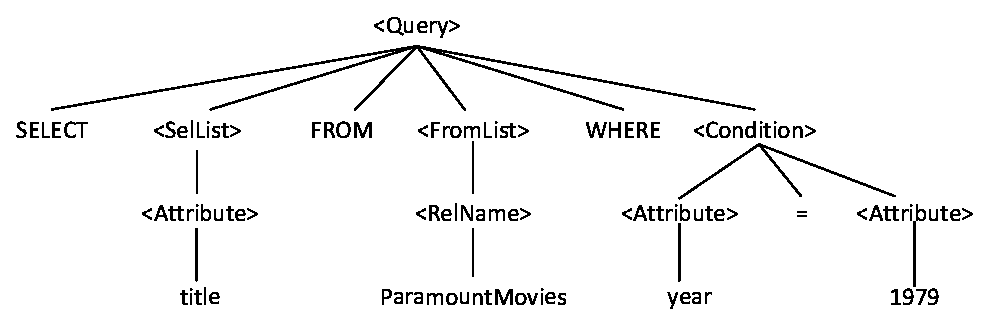
\includegraphics[width=\linewidth]{handout/img/6-view2.eps}
    \caption{查询CST}\label{fig:6-view2}
    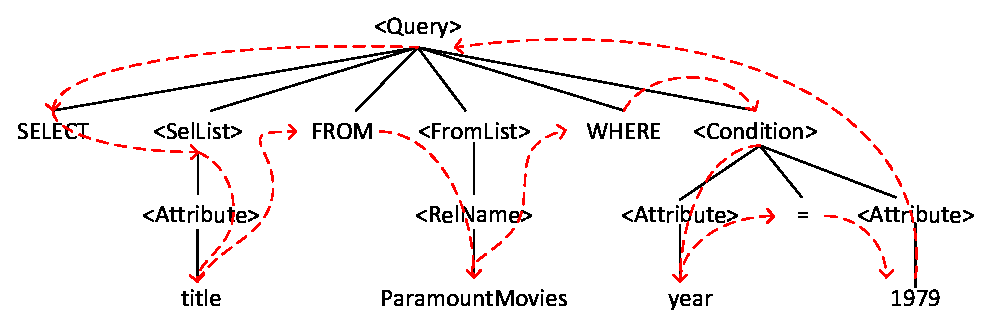
\includegraphics[width=\linewidth]{handout/img/6-view3.eps}
    \caption{深度遍历CST}\label{fig:6-view3}
    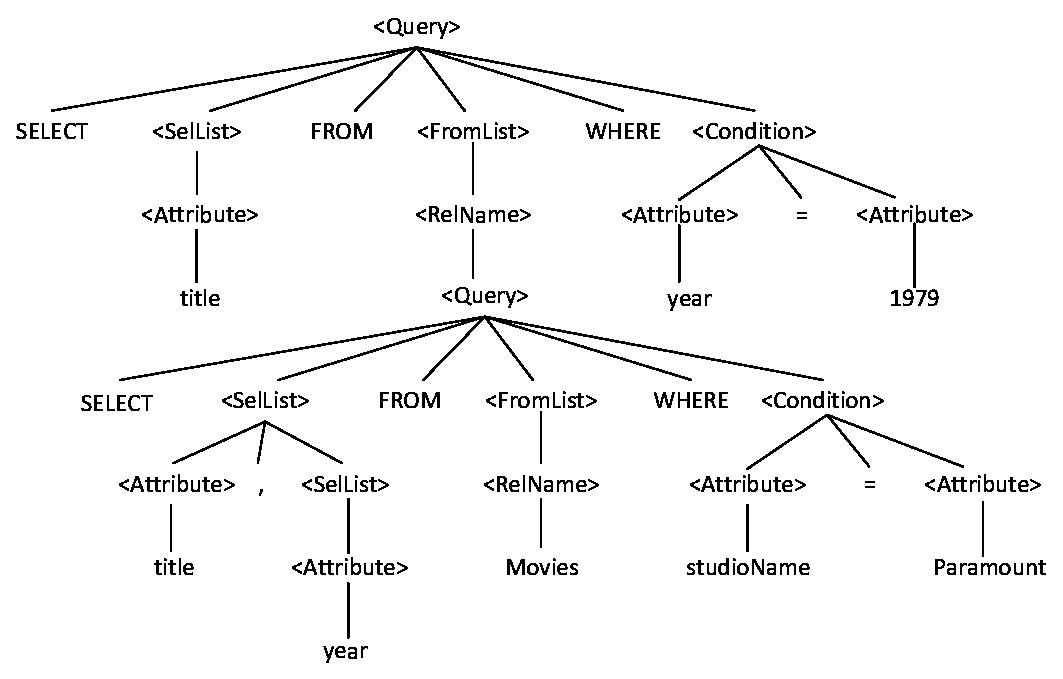
\includegraphics[width=\linewidth]{handout/img/6-view4.eps}
    \caption{视展开CST}\label{fig:6-view4}
\end{figure}

\section{算子表达式特性}

在CST语法树做完预处理后，下一步是要将查询语句翻译成算子表达式，这对应于一个抽象语法树AST。本节先讨论算子表达式的特性，下一节给出AST翻译方法。需要注意，所有关系运算的结果都是关系，换句话说关系代数是一个\emph{关系的封闭系统}。

\subsection{交换律与结合律}

只有双目算子能够考察交换性或结合性，单目算子不需要考虑。如果算子具有交换性与结合性，可将该算子的多次连续操作交换顺序，变换后的算子表达式仍然是等价的，这是一个常见的逻辑优化方案。

多数双目算子具有交换律和结合律，除了差$-$和$\theta$连接，并且适用于bag或者set模型：

\begin{itemize}
    \item $R \times S = S \times R$，$(R\times S) \times T = R\times (S\times T)$
    \item $R \bowtie S = S \bowtie R$，$(R \bowtie S) \bowtie T = R \bowtie (S \bowtie T)$
    \item $R \cup S = S \cup R$，$(R \cup S) \cup T = R \cup (S \cup T)$
    \item $R \cap S = S \cap R$，$(R \cap S) \cap T = R \cap (S \cap T)$
\end{itemize}

考虑等式左边的一个tuple一定会出现在等式的右边，容易证明以上规则。$\theta$连接$\bowtie_C$具有交换律，一般情况下没有结合律，除非$\bowtie_C$的条件在结合后有意义。
\begin{itemize}
    \item $R \bowtie_C S = S \bowtie_C R$
\end{itemize}

\begin{example}
    假设有三个关系$R(a,b)$、$S(b,c)$和$T(c,d)$，表达式$R \bowtie_{R.b>S.b} S \bowtie_{R.a<T.d} T$，条件$R.a<T.d$导致无法结合，因为$R.a$属性只出现在$R$和$R \bowtie_C S$中，$S$本身并没有这个属性。
\end{example}

如果为set模型，对并交操作满足分配律：
\begin{itemize}
    \item $A \cap_S (B \cup_S C) = (A \cap_S B) \cup_S (A \cap_S C)$
\end{itemize}
但是如果底层数据模型为bag，则$\cup_B$和$\cap_B$上不满足分配律。

\subsection{选择操作规则}

绝大多数数据库操作都是根据条件做tuple的查询，这对应于关系上的选择$\sigma$。$\sigma$算子能够穿透大多数双目算子，并且由于选择操作能够大幅降低中间计算结果尺寸，所以关系表达式最常见的逻辑优化规则是下推选择。

\vskip\baselineskip
第一组$\sigma$规则关于交、并、差三种双目算子，这三种算子要求操作关系的属性完全相同：
\begin{itemize}
    \item $\sigma_C(R \cup S) = \sigma_C(R) \cup \sigma_C(S)$
    \item $\sigma_C(R - S) = \sigma_C(R) - S = \sigma_C(R) - \sigma_C(S)$
    \item $\sigma_C(R \cap S) = \sigma_C(R) \cap S = R \cap \sigma_C(S) = \sigma_C(R) \cap \sigma_C(S)$
\end{itemize}

两个关系并的选择，等价于两个关系选择之后再并，注意等式右侧的$\sigma_C$\emph{必须}分别作用在两个操作关系上。

两个关系差的选择，要求$\sigma_C$\emph{必须}作用在被减的关系上。

两个关系交的选择，$\sigma_C$可以作用在任意一个或两个关系上，这使得选择$\sigma$可以在交操作上灵活上推或下推。

\vskip\baselineskip
第二组$\sigma$规则关于其它双目操作，如乘积、连接等，$\sigma$的选择条件不一定能作用到两个关系上，下面的规则假设条件$C(R)$是关于$R$的属性：

\begin{itemize}
    \item $\sigma_C(R \times S) = \sigma_C(R) \times S $
    \item $\sigma_C(R \bowtie S) = \sigma_C(R) \bowtie S$
    \item $\sigma_C(R \bowtie_D S) = \sigma_C(R) \bowtie_D S$
\end{itemize}

上述规则由于具有可交换性，当$C$是关于$S$的，可以写成$R \times \sigma_C(S)$。如果条件$C$关于的属性同时出现在$R,S$，则有：

\begin{itemize}
    \item $\sigma_C(R \times S) = \sigma_C (R) \times \sigma_C(S)$
    \item $\sigma_C(R \bowtie S) = \sigma_C(R) \bowtie \sigma_C(S)$
    \item $\sigma_C(R \bowtie_D S) = \sigma_C(R) \bowtie_D \sigma_C(S)$
\end{itemize}

在上述规则中，要求$\sigma$同时下推到两侧。

\vskip\baselineskip
第三组选择法则是关于\texttt{AND}和\texttt{OR}复合条件：

\begin{itemize}
    \item $\sigma_{C_1 \text{ AND } C_2}(R) = \sigma_{C_1}(\sigma_{C_2}(R)) =  \sigma_{C_2}(\sigma_{C_1}(R))$
    \item $\sigma_{C_1 \text{ OR } C_2}(R) = (\sigma_{C_1}(R)) \cup_S (\sigma_{C_2}(R))$
\end{itemize}

$\sigma$操作是\texttt{AND}连接的两个条件，等价于两个条件的$\sigma$操作的嵌套，并且这两个条件的嵌套顺序无所谓。而$\sigma$操作是\texttt{OR}连接的两个条件，等价于两个条件的$\sigma$操作的set并。当处理bag并时，\texttt{OR}两个条件穿透或后可能导致重复计算。

在生成物理执行计划时，可以考虑使用iterator管道，将多个\texttt{AND}或\texttt{OR}条件连接起来运算，对关系的tuple做选择。也就是说，逻辑执行计划更偏好于组合多层$\sigma$形成一个复杂的选择条件。

\vskip\baselineskip
第四组选择规则将条件扩展为连接，这条规则一般用于处理SQL语句中的\texttt{IN}和\texttt{NOT IN}条件：
\begin{itemize}
    \item $\sigma_{R.a \in S.b}(R) = \pi_R( R \bowtie_{R.a=S.b} S)$
    \item $\sigma_{R.a \overline{\in} S.b}(R) = \pi_R( R \bowtie_{R.a \neq S.b} S)$
    \item $\sigma_{C(R,S) }(R) = \pi_R( R \bowtie_{C} S)$
\end{itemize}
这条规则中，$R.a \in S.b$表示的是两个关系的等值连接，$R.a \overline{\in} S.b$表示两个关系做$\theta$连接，$C(R,S)$在两个关系$R,S$上做选择得到$\theta$连接。一般情况下，第三组规则的左侧更优，但在后文的相关查询中需要将选择变换为$\theta$连接。

\begin{example}
    两个关系$R(a,b)$和$S(b,c)$，考虑算子表达式：
    $$\sigma_{(a=1 \text{ OR } a=3) \text{ AND } b < c}(R \bowtie S)$$
考虑到条件$a=1 \text{ OR } a=3$只作用在$R$上，这个关系表达式变换为：
    $$\sigma_{b < c}(\sigma_{(a=1 \text{ OR } a=3}(R) \bowtie S)$$
进一步，条件$b<c$虽然涉及到$R$的属性，但由于按照$b$做连接，穿透$\bowtie$时可只作用在一侧：
    $$\sigma_{a=1 \text{ OR } a=3}(R) \bowtie \sigma_{b < c}(S)$$
这个例子还暗示着在$\sigma_C(\bowtie)$，如果选择条件$C$涉及到连接属性的处理。
\end{example}

\begin{example}
    这个例子与\examplename\ref{exp:6-view}有关，假设有两个关系：
\begin{lstlisting}[style=verbose]
StarsIn(title, year, starName)
Movies(title, year, length, genre, studioName, producerC#)
\end{lstlisting}
在这两个关系上做查询：
\begin{lstlisting}[style=verbose]
CREATE VIEW Movies0fl996 AS
    SELECT *
    FROM Movies
    WHERE year = 1996;

SELECT starName, studioName
FROM MoviesOf1996 NATURAL JOIN StarsIn;
\end{lstlisting}
    这个查询在两个关系的title和year属性上做连接，view表示为：
    $$\sigma_{year = 1996}(Movies)$$
查询表示为两个关系的自然连接：
    $$\sigma_{year = 1996}(Movies) \bowtie StarsIn$$
    这个算子表达式对应于\figurename\ref{fig:6-select}。先将$\sigma$上推穿透连接，然后再下推得到：
    $$\sigma_{year = 1996}(Movies) \bowtie \sigma_{year = 1996}(StarsIn)$$
    这对应于\figurename\ref{fig:6-select2}。
\end{example}

\begin{figure}[H]
    \centering
    \begin{tikzpicture}
        \node (n1){$\pi_{starName, studioName}$};
        \node[below of=n1] (n2){$\bowtie$};
        \node[below of=n2, xshift = -1cm] (n3){$\sigma_{year=1996}$};
        \node[below of=n2, xshift = 1cm] (n4){StarsIn};
        \node[below of=n3] (n5){Movies};
        \draw[-] (n1) -- (n2);
        \draw[-] (n2) -- (n3);
        \draw[-] (n2) -- (n4);
        \draw[-] (n3) -- (n5);
    \end{tikzpicture}
    \caption{$\sigma$算子下推例子}\label{fig:6-select}
\end{figure}
\begin{figure}[H]
    \centering
    \begin{tikzpicture}
        \node (n1){$\pi_{starName, studioName}$};
        \node[below of=n1] (n2){$\bowtie$};
        \node[below of=n2, xshift = -1cm] (n3){$\sigma_{year=1996}$};
        \node[below of=n2, xshift = 1cm] (n4){$\sigma_{year=1996}$};
        \node[below of=n3] (n5){Movies};
        \node[below of=n4] (n6){StarsIn};
        \draw[-] (n1) -- (n2);
        \draw[-] (n2) -- (n3);
        \draw[-] (n2) -- (n4);
        \draw[-] (n3) -- (n5);
        \draw[-] (n4) -- (n6);
        \end{tikzpicture}
    \caption{$\sigma$算子下推例子2}\label{fig:6-select2}
\end{figure}

在处理$\sigma$下推时，为保证$\sigma$尽可能作用在更多的关系上，优化关系表达式时应该先将$\sigma$上推，然后再下推。

\subsection{投影相关法则}

与下推选择的优化类似，可以下推投影，一般情况下投影也可以减少关系的尺寸。与$\sigma$不同，$\pi$穿透其它算子一般需要引入新的$\pi$，实现中一般会在AST上标注输出属性，根据这个属性可以计算尽可能的做投影。

SQL语句中将属性的表达式也看成投影$\pi_{E \rightarrow x}$，这称为\emph{扩展投影}。扩展投影计算出结果$x$后，将$E$中的属性去掉。例如，扩展投影$\pi_{x+y \rightarrow z}$或者$\pi_{x \rightarrow y}$，实际的SQL语句可能对应于\texttt{SELECT a1+a2 AS b FROM ...}。扩展投影对属性做变换，虽然去掉了$E$中的属性，但并不能保证结果会变小。相对的，将原先的投影定义为\emph{简单投影}，即不涉及属性改名或者没有属性计算的投影$\pi_{E \rightarrow x}$。

对投影做优化的基本思路是：1)~将结果不需要的属性做简单下推投影；2)~扩展投影$\pi_{E \rightarrow x}$尽可能下推；3)~简单投影如果包含在属性$E$中，不能穿透扩展投影。

\begin{itemize}
    \item $\pi_L(R \bowtie S) = \pi_L(\pi_M(R) \bowtie \pi_N(S))$，$M$和$N$是$L$中分别关于$R$和$S$的属性
    \item $\pi_L(R \bowtie_C S) = \pi_L(\pi_M(R) \bowtie_C \pi_N(S))$，$M$和$N$是$L$和$C$中分别关于$R$和$S$的属性
    \item $\pi_L(R \times S) = \pi_L(\pi_M(R) \times \pi_N(S))$，$M$和$N$是$L$中分别关于$R$和$S$的属性
\end{itemize}

上述规则中，$M$和$N$下推投影去除了$\bowtie$、$\bowtie_C$和$\times$运算结果中的无用属性，$\pi_M$和$\pi_N$是两个简单投影。

对于bag模型而言，两个关系的并等价于投影的并：
\begin{itemize}
    \item $\pi_L(R \cup_B S) = \pi_L(R) \cup_B \pi_L(S)$
\end{itemize}
但是set模型没有这个特性。

最后，简单投影可以穿透选择做下推：
\begin{itemize}
    \item $\pi_L(\sigma_C(R)) = \pi_L(\sigma_C(\pi_M(R)))$，$M$是$L$和$C$中依赖的属性
\end{itemize}
这里$M$是简单投影，它表示$L$和$C$中依赖的属性。这个规则没什么用，因为选择会使用iterator管道将投影连接起来处理。

\begin{example}
    以\examplename\ref{exp:6-view}为例，
\begin{lstlisting}[style=verbose]
    CREATE VIEW ParamountMovies AS
        SELECT title, year
        FROM Movies
        WHERE studioName = 'Paramount';
\end{lstlisting}

    这个视表示如下的关系表达式：
    $$\pi_{title, year}(\sigma_{studioName = 'Paramount'}(Movies))$$

    而查询
\begin{lstlisting}[style=verbose]
    SELECT title
    FROM ParamountMovies
    WHERE year = 1979;
\end{lstlisting}

    表示的关系表达式为：
    $$\pi_{title}(\sigma_{year = 1979}(ParamountMovies))$$

\end{example}

\begin{figure}[H]
    \centering
    \begin{tikzpicture}
        \node (n1){$\pi_{title, year}$};
        \node[below of=n1] (n2){$\sigma_{studioName = \text{'Paramount'}}$};
        \node[below of=n2] (n3){Movies};
        \draw[-] (n1) -- (n2);
        \draw[-] (n2) -- (n3);
    \end{tikzpicture}
    \caption{视的AST语法树}\label{fig:6-view-tree}
\end{figure}

\begin{figure}[H]
    \centering
    \begin{tikzpicture}
        \node (n1){$\pi_{title}$};
        \node[below of=n1] (n2){$\sigma_{year = 1979}$};
        \node[below of=n2] (n3){ParamountMovies};
        \draw[-] (n1) -- (n2);
        \draw[-] (n2) -- (n3);
    \end{tikzpicture}
    \caption{包含视的AST语法树}\label{fig:6-view-tree2}
\end{figure}

\begin{figure}[H]
    \centering
    \begin{tikzpicture}
        \node (n1){$\pi_{title}$};
        \node[below of=n1] (n2){$\sigma_{year = 1979}$};
        \node[below of=n2] (n3){$\pi_{title, year}$};
        \node[below of=n3] (n4){$\sigma_{studioName = \text{'Paramount'}}$};
        \node[below of=n4] (n5){Movies};
        \draw[-] (n1) -- (n2);
        \draw[-] (n2) -- (n3);
        \draw[-] (n3) -- (n4);
        \draw[-] (n4) -- (n5);
    \end{tikzpicture}
    \caption{视在语法树上展开}\label{fig:6-view-tree3}
\end{figure}

\begin{figure}[H]
    \centering
    \begin{tikzpicture}
        \node (n1){$\pi_{title}$};
        \node[below of=n1] (n2){$\sigma_{\substack{studioName = \text{'Paramount'} \text{ AND } \\year = 1979}}$};
        \node[below of=n2] (n3){Movies};
        \draw[-] (n1) -- (n2);
        \draw[-] (n2) -- (n3);
    \end{tikzpicture}
    \caption{化简后得到的AST语法树}\label{fig:6-view-tree4}
\end{figure}

\subsection{连接与乘积法则}

根据定义，连接和乘积之间有如下规则：
\begin{itemize}
    \item $R \bowtie_C S = \sigma_C(R \times S)$
    \item $R \bowtie S = \pi_L(\sigma_C(R \times S))$，$C$表示$R$和$S$关系上做连接的同名属性值做相等选择，$L$将两个同名属性去掉一个
\end{itemize}
这里两个规则一般从右向左转化，因为连接比乘积之后的选择要快得多。

如果一个关系自己连接自己：
\begin{itemize}
    \item $R \bowtie R = R$
\end{itemize}

\subsection{副本消除法则}

SQL语言中，一般使用\texttt{DISTICT}关键字表示去重。在在中间计算结果的表上做下推副本消除$\delta$操作可以减小中间表的尺寸，可以加快查询的执行。并且在某些情况下，可以从逻辑上判断直接去掉$\delta$操作：
\begin{itemize}
    \item 聚集存储的关系上声明了主键
    \item set模型上除$\pi$的所有单目操作的计算结果
    \item 当两个关系都是set模型，除$\cup_B$的双目算子计算结果
\end{itemize}

实现上，需要在AST每个节点上设置一个set属性，标记该计算结果是否是set。下推$\delta$可以穿透大多数其它运算：
\begin{itemize}
    \item $\delta(R \times S) = \delta(R) \times \delta(S)$
    \item $\delta(R \bowtie S) = \delta(R) \bowtie \delta(S)$
    \item $\delta(R \bowtie_C S) = \delta(R) \bowtie_C \delta(S)$
    \item $\delta(\sigma_C(R)) = \sigma_C(\delta(R))$
\end{itemize}

对于$\cap$运算，$\delta$可以作用在任意一侧：
\begin{itemize}
    \item $\delta(R \cap S) = \delta(R) \cap S = R \cap \delta(S) = \delta(R) \cap \delta(S)$
\end{itemize}
教材上，交$\cap$是bag模型，其实对set模型也是有效的。这个规则比较有用，与下推$\sigma$类似，它可以先穿越$\cap$上推$\delta$，然后再下推$\delta$。

$\delta$不能穿透$\cup_B$、$-_B$和$\pi$。

\subsection{分组聚合法则}

一般数据库DMBS中，都需要实现\texttt{MIN}、\texttt{MAX}、\texttt{AVG}、\texttt{COUNT}、\texttt{SUM}等几个聚合算法。聚合算法不是普通的函数，它们往往与分组\texttt{GROUP BY}关联，即\texttt{SELECT}的属性列表如果包含了这些聚合函数，则内部实现一般需要分组，而不能看成是扩展投影extending projection。

在实现上，这些聚合函数依赖于分组，即使查询语句中没有显式给出分组\texttt{GROUP BY}，内部也需要根据这些聚合函数的参数做分组。

此外，需要注意的是，聚合计算的结果必然是去重，所以对聚合结果做去重没有意义：
\begin{itemize}
    \item $\delta(\gamma_L(R)) = \gamma_L(R)$，$L$必须包含聚合函数。
\end{itemize}

但是单纯的分组没有上述结论，分组属性$L$中必须包含聚合函数。与上面的结论相对，如果聚合函数是\texttt{MIN}或\texttt{MAX}，去重$\delta$可以穿透分组$\gamma$：
\begin{itemize}
    \item $\gamma_L(R) = \gamma_L(\delta(R))$
\end{itemize}

最后，在\texttt{SELECT}关键字后出现的聚合函数，暗示着类似于投影的语义：
\begin{itemize}
    \item $\gamma_L(R) = \gamma_L(\pi_M(R))$，先对$R$做投影，然后再做分组
\end{itemize}

\begin{example}
    假设两个关系定义如下：
\begin{lstlisting}[style=verbose]
    MovieStar(name, addr, gender, birthdate)
    StarsIn(movieTitle, movieYear, starName)
\end{lstlisting}
    在这两个关系上做如下查询：
\begin{lstlisting}[style=verbose]
    SELECT movieYear, MAX(birthdate)
    FROM MovieStar, StarsIn
    WHERE name = starName
    GROUP BY movieYear;
\end{lstlisting}
    这个查询在\texttt{MovieStar, StarsIn}关系上查找\texttt{name = starName}的元组。虽然在\texttt{GROUP BY}的列表中只有\texttt{movieYear}，但是聚合函数\texttt{MAX}暗示了需要按照\texttt{birthdate}分组。

    这个查询的AST对应于\figurename\ref{fig:6-example-agv}，然后$\sigma(\times(...))$合并成自然连接。\texttt{MAX}函数可以在内部生成一个去重，$\gamma$在内部生成一个投影，得到如\figurename\ref{fig:6-example-agv2}。将$\pi$和$\delta$下推，得到\figurename\ref{fig:6-example-agv3}。

    在\figurename\ref{fig:6-example-agv2}，先在内部生成一个$\pi$，然后再生成一个$\delta$，因为$\delta$无法穿透$\pi$。
\end{example}

\begin{figure}[H]
    \centering
    \begin{tikzpicture}
        \node (n1){$\gamma_{movieYear, \text{ MAX}(birthdate)}$};
        \node[below of=n1] (n2){$\sigma_{name=starName}$};
        \node[below of=n2] (n3){$\times$};
        \node[below of=n3, xshift=-1cm] (n4){MovieStar};
        \node[below of=n3, xshift=1cm] (n5){StarsIn};
        \draw[-] (n1) -- (n2);
        \draw[-] (n2) -- (n3);
        \draw[-] (n3) -- (n4);
        \draw[-] (n3) -- (n5);
    \end{tikzpicture}
    \caption{分组聚合示例}\label{fig:6-example-agv}
\end{figure}

\begin{figure}[H]
    \centering
    \begin{tikzpicture}
        \node (n0){$\gamma_{movieYear, \text{ MAX}(birthdate)}$};
        \node[below of=n0] (n1){$\delta$};
        \node[below of=n1] (n2){$\pi_{movieYear, birthdate}$};
        \node[below of=n2] (n3){$\bowtie_{name=starName}$};
        \node[below of=n3, xshift=-1cm] (n4){MovieStar};
        \node[below of=n3, xshift=1cm] (n5){StarsIn};
        \draw[-] (n0) -- (n1);
        \draw[-] (n1) -- (n2);
        \draw[-] (n2) -- (n3);
        \draw[-] (n3) -- (n4);
        \draw[-] (n3) -- (n5);
    \end{tikzpicture}
    \caption{分组聚合示例2}\label{fig:6-example-agv2}
\end{figure}

\begin{figure}[H]
    \centering
    \begin{tikzpicture}
        \node (n1){$\gamma_{movieYear, \text{ MAX}(birthdate)}$};
        \node[below of=n1] (n3){$\bowtie_{name=starName}$};
        \node[below of=n3, xshift=-1.5cm] (n4){$\delta$};
        \node[below of=n3, xshift=1.5cm] (n5){$\delta$};
        \node[below of=n4] (n6){$\pi_{birthdate,name}$};
        \node[below of=n5] (n7){$\pi_{movieYear,starName}$};
        \node[below of=n6] (n8){MovieStar};
        \node[below of=n7] (n9){StarsIn};
        \draw[-] (n1) -- (n3);
        \draw[-] (n3) -- (n4);
        \draw[-] (n3) -- (n5);
        \draw[-] (n4) -- (n6);
        \draw[-] (n5) -- (n7);
        \draw[-] (n6) -- (n8);
        \draw[-] (n7) -- (n9);
    \end{tikzpicture}
    \caption{分组聚合示例3}\label{fig:6-example-agv3}
\end{figure}

\section{算子表达式生成}

SQL语言按照生成式被翻译成CST语法树，在经过类型检查等预处理后，下一步需要将CST变换成抽象语法树AST，AST对应于关系算子表达式。c语言的CST与AST差异不大，但SQL语言中二者有很大差异。在编译原理中，CST转换为AST属于语义分析的范畴，通常采用语法制导翻译。

\subsection{SQL语言}

这里先回顾SQL语言，更详细的内容参见文献\cite{Ullman1998A}第6章。

\subsubsection*{\texttt{SELECT-FROM-WHERE}}

一条简单的\texttt{SELECT-FROM-WHERE}查询语句如下：

\begin{lstlisting}[style=verbose]
    SELECT *
    FROM Movies
    WHERE studioName = 'Disney' AND year = 1990;
\end{lstlisting}

在这条语句中，各个部分的含义是：
\begin{itemize}
    \item \texttt{FROM}指出查询算子作用的关系
    \item \texttt{WHERE}指出查询的条件
    \item \texttt{SELECT}指定输出的字段，对应于投影算子
\end{itemize}

这三个部分与\ref{sec:6-sql}的SQL语法子集中\texttt{<SelectList>}、\texttt{<FromList>}、\texttt{<Con\-dition>}非终止符是对应的。

在SQL-99中，\texttt{SELECT}语句可以利用\texttt{AS}变换输出的属性名称：
\begin{lstlisting}[style=verbose]
    SELECT title, length*0.016667 AS length
    FROM Movies
    WHERE studioName = 'Disney' AND year = 1990;
\end{lstlisting}

\texttt{WHERE}后部的条件是最复杂的部分，SQL-99支持逻辑、算术运算、模式匹配等。

\subsubsection*{\texttt{GROUP BY, ORDER BY}}

使用排序和分组的语句示例如下：
\begin{lstlisting}[style=verbose]
    SELECT *
    FROM Movies
    WHERE studioName = 'Disney' AND year = 1990
    ORDER BY length, title;

    SELECT *
    FROM Movies
    WHERE year = 1990
    GROUP BY sudioName;
\end{lstlisting}

\texttt{GROUP BY, ORDER BY}后面指明分组和排序的属性列表。聚合操作支持\texttt{MIN, MAX, AVG, COUNT, SUM}，这些聚合函数出现在\texttt{SELECT}后的列表中。

\subsubsection*{$\times, \bowtie$}

SQL使用\texttt{FROM}中给出需要处理的多个关系名表示积$\times$。SQL专门设计自然连接\texttt{NATURAL JOIN}和外连接\texttt{OUTER JOIN}关键字，但很少使用，一般表示为乘积，然后由SQL编译器优化为连接或者$\theta$连接。
\begin{lstlisting}[style=verbose]
    SELECT name
    FROM Movies, MovieExec
    WHERE title = 'Star Weirs' AND producerC# = cert#;
\end{lstlisting}

上面的语句中由于使用条件\texttt{producerC\# = cert\#}，表示两个关系的自然连接。所以，要区分出积和连接，是SQL解析器的任务。并且，从SQL语言来看，并没有强制规定算子一定是双目的，可以是多目的。

\subsubsection*{$-, \cap, \cup$}

交并差在SQL中使用关键字\texttt{INTERSECT, UNIION, EXCEPT}表示，如下面的例子：
\begin{lstlisting}[style=verbose]
    (SELECT name, address
     FROM MovieStar
     WHERE gender = 'F'))
    INTERSECT
    (SELECT name, address
     FROM MovieExec
     WHERE netWorth > 10000000);
\end{lstlisting}

\subsubsection*{嵌套子查询}

SQL语法是生成式表述，它支持\texttt{SELECT-FROM-WHERE}语法结构嵌套使用，具体来说嵌套子查询只出现在两个位置：\texttt{FROM}和\texttt{WHERE}。

\begin{itemize}
    \item 子查询的结果可能是一个标量，这个标量可以参与外层查询语句中\texttt{WHERE}中的逻辑表达式计算。
    \item 子查询的结果如果是一个关系，这个关系可以用在\texttt{FROM}和\texttt{WHERE}中。
\end{itemize}

如果查询条件作用在键上，并且\texttt{SELECT}指定只选择一个属性，由于只能选中一行的一个属性，输出结果一定是标量。

\begin{example}
    有两个关系，
\begin{lstlisting}[style=verbose]
Movies(title, year, length, genre, studioName, producerC#)
MovieExec(name, address, cert#, netWorth)
\end{lstlisting}

\texttt{MovieExec}关系的主键是\texttt{cert\#}，然后在这两张表上查询Star Wars电影的制片商
\begin{lstlisting}[style=verbose]
    SELECT name
    FROM Movies, MovieExec
    WHERE title = 'Star Wars' AND producerC# = cert#;
\end{lstlisting}

换一个角度考虑这个问题，由于\texttt{producerC\#}是\texttt{MovieExec}的外键，可以在\texttt{WHERE}条件中指定相等：
\begin{lstlisting}[style=verbose]
    SELECT name
    FROM MovieExec
    WHERE cert# =
        (SELECT producerC#
         FROM Movies
         WHERE title = 'Star Wars');
\end{lstlisting}

后者的的执行效果要好很多，因为可以使用\texttt{Movies}和\texttt{MovieExec}的索引直接输出，而前者如果优化没做好，会使用乘积来处理。
\end{example}

在\ref{sec:6-sql}的语法定义中，\texttt{LIKE}也是作用在单个属性上，它如果嵌套子查询也要求是一个标量。\texttt{IN}后可以嵌套一个子查询，子查询的输出为一个关系。

\begin{example}
    有三张表，
\begin{lstlisting}[style=verbose]
Movies(title, year, length, genre, studioName, producerC#)
StarsIn(movieTitle, movieYear, starName)
MovieExec(name, address, cert#, netWorth)
\end{lstlisting}

在这三张表上查询Harrison Ford参演影片的片商：
\begin{lstlisting}[style=verbose]
    SELECT name
    FROM MovieExec
    WHERE cert# IN
        (SELECT producerC#
         FROM Movies
         WHERE (title, year) IN
            (SELECT movieTitle, movieYear
             FROM StarsIn
             WHERE starName = 'Harrison Ford')
        );
\end{lstlisting}

整个查询嵌套了三层，最内层先在\texttt{StarsIn}上查询Harrison Ford参演的影片，然后在\texttt{Movies}上查询影片的生产商，最后在\texttt{MovieExec}上查询片商的名称。这个查询等价于：
\begin{lstlisting}[style=verbose]
    SELECT name
    FROM MovieExec, Movies, Starsln
    WHERE cert# = producerC# AND
        title = movieTitle AND
        year = movieYear AND
        starName = 'Harrison Ford';
\end{lstlisting}
\end{example}

\subsubsection*{名字解析}

SQL中的名字包括：属性名、表名或者视名。SQL名字解析原则如下：
\begin{itemize}
    \item 在解析SQL语句之前，已创建的表和视，及其属性可见；
    \item \texttt{SELECT-FROM-WHERE}构成一个名字scope；\texttt{FROM}后用\texttt{AS}声明的表实例在这个scope内可见；
    \item 在嵌套子查询中，外层scope的名字可见；
\end{itemize}

\subsection{简单算子表达式构造} \label{sec:6-convert-relation-exp}

\texttt{SELECT-FROM-WHERE}的SQL语法结构包含了投影$\pi$，选择$\sigma$以及乘积$\times$，CST语法树可以利用语法制导翻译出一个$\pi_D(\sigma_C(R \times S \times ...))$或$\gamma_D(\sigma_C(R \times S \times ...))$表达式，其中属性列表$D$由\texttt{SELECT}节点属性给出，条件$C$由\texttt{WHERE}节点属性给出。

这里先讨论最简单的情况：假设\texttt{FROM}和\texttt{WHERE}中没有子查询。条件$C$和$D$的构造是容易的：
\begin{itemize}
    \item 如果只有一个关系则去掉$\times$
    \item 条件$C$即为\texttt{WHERE}中的逻辑表达式
    \item 投影$D$为\texttt{SELECT}中的扩展投影
\end{itemize}

\begin{figure}[H]
    \centering
    \begin{tikzpicture}[node distance = 1cm]
        \node                                   (pi)    {$\pi_D$};
        \node [below of= pi]                    (sigma) {$\sigma_C$};
        \node [below of= sigma]                 (times) {$\times$};
        \node [below of= times, xshift = -1cm]  (R)     {$R$};
        \node [right of= R]                     (S)     {$S$};
        \node [below of= times, xshift = 1cm]   (dot)   {$...$};
        \path (pi)      edge    (sigma);
        \path (sigma)   edge    (times);
        \path (times)   edge    (R);
        \path (times)   edge    (S);
        \path (times)   edge    (dot);
    \end{tikzpicture}
    \caption{将select-from-where构造基本关系表达式}\label{fig:6-construct-relation}
\end{figure}

在实现中，$\times$可以拥有1个或多个子节点，在优化时利用$\sigma_D(R \times S) = R \bowtie_{D} S$将去除$\times$。举例而言，\examplename\ref{exp:6-parse-tree2}的查询语句，它的语法树被翻译成表达式如\figurename\ref{fig:6-example}。

\begin{figure}[H]
    \centering
    \begin{tikzpicture}
        \node (n1){$\pi_{movieTitle}$};
        \node[below of=n1] (n2){$\sigma_{\substack{starName=Name \text{ AND } \\ birthdate \text{ LIKE } '\%1960'}}$};
        \node[below of=n2] (n3){$\times$};
        \node [below of= n3, xshift = -1cm]  (R){StarsIn};
        \node [right of= R, xshift = 1cm] (S){MovieStar};
        \draw[-] (n1) -- (n2);
        \draw[-] (n2) -- (n3);
        \draw[-] (n3) -- (R);
        \draw[-] (n3) -- (S);
    \end{tikzpicture}
    \caption{\examplename\ref{exp:6-parse-tree2}查询语句被翻译为关系表达式}\label{fig:6-example}
\end{figure}

\subsection{\texttt{FROM}嵌套子查询}

当\texttt{FROM}中包含子查询，这个子查询生成的中间结果作为$\times$的一个子节点进行处理，类似于view替换。

\begin{example}\label{exp:6-parse-tree3}
    假设有三个关系定义如下：
\begin{lstlisting}[style=verbose]
    Movies(title, year, length, genre, studioName, producerC#)
    StarsIn(movieTitle, movieYear, starName)
    MovieExec(name, address, cert#, netWorth)
\end{lstlisting}

    在这三个关系上做查询
\begin{lstlisting}[style=verbose]
    SELECT name
    FROM MovieExec, (SELECT producerC#
                     FROM Movies, StarsIn
                     WHERE title = movieTitle AND
                           year = movieYear AND
                           starName = 'Harrison Ford'
                    ) Prod
    WHERE cert# = Prod.producerC#;
\end{lstlisting}

    这条查询语句的算子表达式为\figurename\ref{fig:6-example3}。
\end{example}

\begin{figure}[H]
    \centering
    \begin{tikzpicture}
        \node (n1){$\pi_{name}$};
        \node[below of=n1] (n2){$\sigma_{cert\# = Prod.producerC\#}$};
        \node[below of=n2] (n3){$\times$};
        \node[below of= n3, xshift = -1cm]  (n4){MovieExec};
        \node[right of= R, xshift = 1cm] (n5){$\pi_{producerC\#}$};
        \node[below of=n5] (n6){$\sigma_{\substack{title = movieTitle \text{ AND } \\
        year = movieYear \text{ AND } \\
        starName = \text{'Harrison Ford'}}}$};
        \node[below of=n6, xshift = -1cm] (n7){Movies};
        \node[right of=n7, xshift = 1cm] (n8){StarsIn};
        \draw[-] (n1) -- (n2);
        \draw[-] (n2) -- (n3);
        \draw[-] (n3) -- (n4);
        \draw[-] (n3) -- (n5);
        \draw[-] (n5) -- (n6);
        \draw[-] (n6) -- (n7);
        \draw[-] (n6) -- (n8);
    \end{tikzpicture}
    \caption{\examplename\ref{exp:6-parse-tree3}查询语句被翻译为算子表达式}\label{fig:6-example3}
\end{figure}

\subsection{\texttt{WHERE}属性嵌套子查询}

\texttt{WHERE}后部是选择条件，这个选择条件是$\sigma$算子的下标。\texttt{WHERE}的条件表达式可能嵌套一个子查询，这个子查询在AST中被处理成$\sigma$算子的属性，教材上将它处理成一个\emph{双参}$\sigma$。

\begin{example}\label{exp:6-parse-tree4}
    以\examplename\ref{exp:6-parse-tree}为例，\texttt{WHERE}后的条件\texttt{starName IN}被处理成$\sigma$算子的属性：
    $$\pi_{movieTitle}(\sigma_{starName \in \pi_{name}(\sigma_{birthdate \text{ LIKE } '\%*.1960'}(MovieStar))}(StarsIn))$$
    其中$\pi_{name}(\sigma_{birthdate \text{ LIKE } '\%*.1960'}(MovieStar))$对应于一个中间结果关系，name是这个中间结果的一个属性，表示为\figurename\ref{fig:6-example4}。至于转化为$\times$是一个优化问题，由于$name \in$可以表示为一个等值连接，这个表达式最终被转化为\ref{fig:6-example5}。
    \end{example}

\begin{figure}[H]
    \centering
    \begin{tikzpicture}
        \node (n1){$\pi_{movieTitle}$};
        \node[below of=n1] (n2){$\sigma$};
        \node[below of=n2] (n3){StarsIn};
        \node[right of=n2, xshift=1.5cm] (n41){\tiny$starName \in$};
        \node[right of=n41, xshift=0.2cm] (n4){\tiny$\pi_{name}$};
        \node[below of=n4] (n5){$\sigma_{birthdate \text{ LIKE '\%.1960'}}$};
        \node[below of=n5] (n6){MovieStar};
        \draw[-] (n1) -- (n2);
        \draw[-] (n2) -- (n3);
        \draw[dashed] (n2) -- (n41);
        \draw[-] (n4) -- (n5);
        \draw[-] (n5) -- (n6);
    \end{tikzpicture}
    \caption{\examplename\ref{exp:6-parse-tree4}查询语句被翻译为算子表达式}\label{fig:6-example4}
\end{figure}

\begin{figure}[H]
    \centering
    \begin{tikzpicture}
        \node (n1){$\pi_{movieTitle}$};
        \node[below of=n1] (n2){$\substack{\bowtie \\ starName=name}$};
        \node[below of=n2, xshift=-1cm] (n3){StarsIn};
        \node[right of=n3, xshift=1cm] (n4){$\pi_{name}$};
        \node[below of=n4] (n5){$\sigma_{birthdate \text{ LIKE '\%.1960'}}$};
        \node[below of=n5] (n6){MovieStar};
        \draw[-] (n1) -- (n2);
        \draw[-] (n2) -- (n3);
        \draw[-] (n2) -- (n4);
        \draw[-] (n4) -- (n5);
        \draw[-] (n5) -- (n6);
    \end{tikzpicture}
    \caption{\examplename\ref{exp:6-parse-tree4}查询语句优化后的算子表达式}\label{fig:6-example5}
\end{figure}

\subsection{相关子查询}

子查询的翻译会碰到一个问题：子查询有可能会引用外部名字，这个名字可能是外部的关系或者属性。如果子查询没有引用外部名字，称子查询是\emph{无关的}，否则称为\emph{相关的}。

与c语言不同，SQL中的名字可以定义在\texttt{SELECT}、\texttt{FROM}或者\texttt{WHERE}中。名字的scope在整个\texttt{SELECT-FROM-WHERE}结构内有效，内层子查询可以引用外部名字。CST在预处理阶段还应该有一个工作：收集该层结构上的所有变量，然后在\texttt{<Query>}节点上标注。

如果内层嵌套子查询引用的外部名字是关系，则意味着这个关系会参与内层嵌套子查询的计算，按照前述的嵌套子查询方式处理。如果引用的是外部关系的属性，这个外部属性一般出现在内层嵌套子查询的\texttt{WHERE}部分，此时问题实质是：内层子查询可能引用外部关系的属性作为条件判断，但是计算总是从内层开始，而外部关系的属性值是未知的。

当内层嵌套子查询的\texttt{WHERE}条件判断出现外部关系的属性，需要利用$\sigma_{C(R,S)}(R) = R \bowtie_{C} S$将选择转化为一个$\theta$连接。

\begin{example}
    假设有两个关系：
\begin{lstlisting}[style=verbose]
    StarsIn(movieTitle, movieYear, starName)
    MovieStar(name, address, gender, birthdate)
\end{lstlisting}

    在\texttt{StarsIn}和\texttt{MovieStar}关系上做如下查询：
\begin{lstlisting}[style=verbose]
    SELECT DISTINCT m1.movieTitle, m1.movieStar
    FROM StarsIn m1
    WHERE m1.movieYear - 40 <= (
        SELECT AVG(s.birthdate)
        FROM StarsIn m2, MovieStar s
        WHERE m2.starName = s.name AND
            m1.movieTitle = m2.movieTitle AND
            m1.movieYear = m2.movieYear
    );
\end{lstlisting}

    这条SQL命令查询影星的平均年龄在40岁之下的电影。先看内部嵌套子查询，这个子查询从StarsIn和MovieStar两个表的连接做查询，其余条件使用了外部变量m1，计算平均生日，然后再利用平均生日去计算外部查询。
    \begin{gather}
        a=m1.movieTitle \notag \\
        b=m1.movieStar \notag \\
        c=m2.starName \notag \\
        d=s.name \notag \\
        e=m2.movieTitle \notag \\
        f=m1.movieYear \notag \\
        g=m2.movieYear \notag \\
        h=s.birthdate \notag \\
        i=\sigma_{a=e \text{ AND } f=g \text{ AND } c=d }(m2 \times s) \notag \\
        j=\gamma_{AVG(h)}(i) \notag \\
        k=\delta(\pi_{a,b}(\sigma_{f-40 \le j}(m1))) \notag
    \end{gather}
    由于\texttt{m1.movie\-Year = m2.movieYear}，可以将之处理成为一个自然连接，得到\figurename\ref{fig:6-example6}。条件$j(m1,m2,s)$处理成一个$\theta$连接，\figurename\ref{fig:6-example7}。
    \begin{gather}
        k_2=\delta(\pi_{a,b}(\sigma_{f-40 \le h}(m1 \times i))) \notag
    \end{gather}
    然后将选择算子$\sigma_{a=e \text{ AND } f=g}$上移与$\times$结合得到连接算子，得到\figurename\ref{fig:6-example8}。$\pi$算子上移后，得到：
    $$m1 \bowtie (m2 \bowtie s)$$
    由于$m1,m2$是同一个关系，最后得到$m1 \bowtie s$，如\figurename\ref{fig:6-example9}。
\end{example}

\begin{figure}[H]
    \centering
    \begin{tikzpicture}
        \node (n0){$\delta$};
        \node[below of=n0] (n1){$\pi_{m1.movieTitle,m1.movieYear}$};
        \node[below of=n1] (n2){$\sigma$};
        \node[below of=n2] (n3){StarsIn m1};
        \node[right of=n2, xshift=1.5cm] (n4){$m1.movieYear-40 \le$};
        \node[right of=n4, xshift=2.2cm] (n5){$\gamma_{AVG(s.birthdate)}$};
        \node[below of=n5] (n6){$\sigma_{\substack{m1.movieTitle = m2.movieTitle \text{ AND }\\ m1.movieYear = m2.movieYear}}$};
        \node[below of=n6] (n7){$\substack{\bowtie \\m2.starName = s.name}$};
        \node[below of=n7, xshift=-1cm] (n8){StarsIn m2};
        \node[right of=n8, xshift=1cm] (n9){MovieStar s};
        \draw[-] (n0) -- (n1);
        \draw[-] (n1) -- (n2);
        \draw[-] (n2) -- (n3);
        \draw[dashed] (n2) -- (n4);
        \draw[-] (n5) -- (n6);
        \draw[-] (n6) -- (n7);
        \draw[-] (n7) -- (n8);
        \draw[-] (n7) -- (n9);
    \end{tikzpicture}
    \caption{相关嵌套子查询举例}\label{fig:6-example6}
\end{figure}

\begin{figure}[H]
    \centering
    \begin{tikzpicture}
        \node (n0){$\delta$};
        \node[below of=n0] (n1){$\pi_{m1.movieTitle,m1.movieYear}$};
        \node[below of=n1] (n21){$\sigma_{m1.movieYear-40 \le AVG(s.birthdate)}$};
        \node[below of=n21] (n2){$\times$};
        \node[below of=n2] (n3){StarsIn m1};
        \node[right of=n3, xshift=3cm] (n6){$\sigma_{\substack{m1.movieTitle = m2.movieTitle \text{ AND }\\ m1.movieYear = m2.movieYear}}$};
        \node[below of=n6] (n7){$\substack{\bowtie \\m2.starName = s.name}$};
        \node[below of=n7, xshift=-1cm] (n8){StarsIn m2};
        \node[right of=n8, xshift=1cm] (n9){MovieStar s};
        \draw[-] (n0) -- (n1);
        \draw[-] (n1) -- (n21);
        \draw[-] (n21) -- (n2);
        \draw[-] (n2) -- (n3);
        \draw[-] (n2) -- (n6);
        \draw[-] (n6) -- (n7);
        \draw[-] (n7) -- (n8);
        \draw[-] (n7) -- (n9);
    \end{tikzpicture}
    \caption{相关嵌套子查询举例2}\label{fig:6-example7}
\end{figure}

\begin{figure}[H]
    \centering
    \begin{tikzpicture}
        \node (n0){$\delta$};
        \node[below of=n0] (n1){$\pi_{m1.movieTitle,m1.movieYear}$};
        \node[below of=n1] (n21){$\sigma_{m1.movieYear-40 \le abd}$};
        \node[below of=n21] (n2){$\bowtie_{\substack{m1.movieTitle = m2.movieTitle \text{ AND }\\ m1.movieYear = m2.movieYear}}$};
        \node[below of=n2] (n3){StarsIn m1};
        \node[right of=n3, xshift=3cm] (n6){$\gamma_{\substack{m2.movieTitle,\\ m2.movieYear, \\AVG(s.birthdate) \rightarrow abd}}$};
        \node[below of=n6] (n7){$\substack{\bowtie \\m2.starName = s.name}$};
        \node[below of=n7, xshift=-1cm] (n8){StarsIn m2};
        \node[right of=n8, xshift=1cm] (n9){MovieStar s};
        \draw[-] (n0) -- (n1);
        \draw[-] (n1) -- (n21);
        \draw[-] (n21) -- (n2);
        \draw[-] (n2) -- (n3);
        \draw[-] (n2) -- (n6);
        \draw[-] (n6) -- (n7);
        \draw[-] (n7) -- (n8);
        \draw[-] (n7) -- (n9);
    \end{tikzpicture}
    \caption{相关嵌套子查询举例3}\label{fig:6-example8}
\end{figure}

\begin{figure}[H]
    \centering
    \begin{tikzpicture}
        \node (n0){$\delta$};
        \node[below of=n0] (n1){$\pi_{m2.movieTitle,m2.movieYear}$};
        \node[below of=n1] (n2){$\sigma_{m2.movieYear-40 \le abd}$};
        \node[below of=n2] (n3){$\gamma_{\substack{m2.movieTitle,\\ m2.movieYear, \\AVG(s.birthdate) \rightarrow abd}}$};
        \node[below of=n3] (n4){$\substack{\bowtie \\m2.starName = s.name}$};
        \node[below of=n4, xshift=-1cm] (n5){StarsIn m2};
        \node[below of=n4, xshift=1cm] (n6){MovieStar s};
        \draw[-] (n0) -- (n1);
        \draw[-] (n1) -- (n2);
        \draw[-] (n2) -- (n3);
        \draw[-] (n3) -- (n4);
        \draw[-] (n4) -- (n5);
        \draw[-] (n4) -- (n6);
    \end{tikzpicture}
    \caption{相关嵌套子查询举例4}\label{fig:6-example9}
\end{figure}

\section{逻辑优化}

在语义分析完毕后，CST转化为一个AST。这个AST的内部节点为各种算子，叶子节点为存储在磁盘上的关系，每个节点上会标注输出属性列表、是否是set模型。与每个子查询\texttt{SELECT-FROM-WHERE}对应，会在该子查询的根节点标注名字列表，实现中可以考虑引入一个特定的节点$\alpha$表示。

逻辑优化的目标至少有两个：1)~变换算子表达式，得到开销最小的算子表达式；2)~消除相关子查询。后者可以通过检查AST的节点属性判断，当发现一个嵌套子查询引用外部关系的属性，可以判断为相关子查询。——这种情况只能出现在\texttt{WHERE}之后，如果出现在\texttt{SELECT}后，CST类型检查会报错。

除了处理相关子查询correlated subquery，逻辑优化的目标是得到开销最小的算子表达式，这要求准确度量一个段子表达式的开销。以\figurename\ref{fig:6-example9}为例计算开销，从根出发，$\delta$建连索引可以支持tuple管道，$\pi$算子支持tuple管道，主要问题在于$\gamma$和$\bowtie$。参考\tablename\ref{tbl:operator-two-pass}，一个算子表达式的开销主要考虑的是$\gamma, -, \times, \bowtie, \bowtie_C$这些不支持tuple管道或者$M$兜不住的算子。进一步，\figurename\ref{fig:6-example9}中$m2 \bowtie s$的开销是可知的，但问题是它的计算结果大小是未知的，从而$\gamma$的开销是未知的。

教材中，估算这个中间计算结果的开销需要利用$V(R,a)$参数，这个统计值由数据库系统周期性的在空闲时扫描全表建立。

逻辑优化的主要方案由两种：1)~直观的规则变换，从原始的AST出发，利用规则对AST上的算子做变换；2)~采用动态规划法，枚举所有规则对算子表达式做变换，估算变换后的算子表达式开销。后者能够得到全局最优解，前者只能得到一个局部最优解。但是，动态规划法存在两个方面的问题：1)~中间计算结果的估算不准确，$V(R,a)$统计值的维护成本很高。2)~存在$R \cap R=R$这样的冗余公式，使得等价算子表达式无穷多，必须将等价算子表达式的解空间降下来。

\subsection{中间结果开销估计}

上一章中，度量一个操作的算法性能主要有两个指标：磁盘IO数量和内存约束。与通常的算法性能评估一致，磁盘IO数量以幂的阶次$O()$来评估。但需要注意，采用多项式幂来评估算子表达式性能，精度是不够的。这也是本小节的目的，希望更精确地给出算子实现算法的性能。

估计中间关系大小需要满足如下几个要求，其中一致性估计比较难以满足。
\begin{itemize}
    \item 准确
    \item 方便
    \item 一致，操作可以采用不同的实现算法，但是中间关系的结果是不变的
\end{itemize}

\subsubsection*{估计投影大小}

不论是简单投影还是扩展投影，都可以准确地推算出$\pi$结果的大小，只是扩展投影要创建新的属性，有可能会增加结果尺寸。

\subsubsection*{估计选择大小}

$\sigma_C$选择的条件有几种：相等、不等、不同。

$\sigma_=$得到的中间结果可以估计为$T(S)=T(R)/V(R,A)$，即对关系$R$的属性$A$做相等选择，平均选择概率是总的记录数目除以属性$A$的不同个数。

$\sigma_<$得到的中间结果可以估计为$T(S)=T(R)/3$，就是$1/3$左右。

$\sigma_{\neq}$得到的中间结果估计为$T(S)=T(R)(V(R,A)-1)/V(R,A)$，即属性$A$的数目减1的概率。

当$\sigma_C$是由\texttt{AND}连接的多个条件，我们可以将之处理为多个$\sigma$级联。这个级联的顺序无所谓，反正结果都是一样的。

$\sigma_{C_1 \text{ OR } C_2}(R)$，如果$C_1$和$C_2$两个条件互相独立，$R$有$n$个记录，$C_1$选择得到了$m_1$个记录，$C_2$选择得到了$m_2$个记录，结果关系的大小为$n(1-(1-m_1/n)(1-m_2/n))$。

$\sigma_{\text{NOT } C}(R)$的中间结果大小为$T(R)$减去$\sigma_C$的估计值。

更准确的估计需要精确掌握$R$关于属性$A$的概率分布，这并不容易做到。教材上介绍了Zipf分布，简单地说，就是2/8律。

实际的选择估计还需要判断条件是否为false，从而导致中间结果大小为0。

\subsubsection*{估计连接的大小}

这里只考虑自然连接，其余的连接按如下规则处理：
\begin{itemize}
    \item 相等连接等同于自然连接，需要考虑的指数属性名字的不同
    \item $\theta$连接等同于$\times$算子后跟一个$\delta$算子，笛卡尔积产生的记录数等于两个关系的记录数目的乘积
\end{itemize}

计算$R(X,Y) \bowtie S(Y,Z)$的大小，主要问题是$Y$在$R$和$S$中是何种关系，例如：
\begin{itemize}
    \item 如果$R$和$S$中的$Y$不相交，则$T(R\times S)=0$
    \item 如果$Y$是$R$的主键，是$S$的外键，则$T(R\times S)=T(R)$
    \item 如果$R$和$S$中的$Y$都相同，则$T(R\times S)=T(R)T(S)$
\end{itemize}

上述例子中，计算连接时结果存在巨大差异。为应付一般性的场景，做如下假设：
\begin{itemize}
    \item 值集包容，如果$V(R,Y) \le V(S,Y)$，则$R$中每个$Y$值都会出现在$S$中。
    \item 值集保持，如果属性$A$是$R$属性但不是$S$的属性，则$V(R\bowtie S,A)=V(R,A)$。
\end{itemize}
值集包容假设并不一定成立，但是在多数情况下是成立的，并且满足$Y$是$S$的主键$R$的外键的情况。值集保持假设也可能不成立，但是对于$Y$是$S$的主键$R$的外键的情况是满足的。值集保持假设在绝大多数情况下是成立的，仅当\emph{dangling tuple}的情况才会出错，即$R$和$S$在属性$Y$上不相交。基于上述假设，自然连接的估计为$T(R\bowtie S)=T(R)T(S)/max(V(R,Y),V(S,Y))$。

当$Y$是多个属性时，估计为$T(R\bowtie S)=T(R)T(S)/max(V(R,y_1),V(S,y_2))$，其中$y_1$使得$V(R,y_1)$最大，$y_2$使得$V(S,y_2)$最大。

多个自然连接的情况$S=R_1 \bowtie R_2 \bowtie ... \bowtie R_n$，先将$T(R_i)$相乘，然后找到所有出现过两次的属性$A$，将乘积除以$V(R_i,A)$（最小的$V(R_i,A)$除外）。

\subsubsection*{估计其它操作大小}

处理前面介绍的投影$\pi$、选择$\sigma$和连接$\bowtie$三种操作外，其余的操作只能凭经验给出估计。

$R \cup_B S$相对容易，$T(R)+T(S)$。$R \cup_S S$不好估计，它的最大值是$T(R)+T(S)$，最小值是$max(T(R),T(S))$，教材中的估计值是$(T(R)+T(S)+max(T(R),T(S)))/2$。

$R \cap S$的最小值是0，最大值是$min(T(R),T(S))$，估计值为$min(T(R),T(S))/2$。

$R-S$的结果在$T(R)$和$T(R)-T(s)$之间，教材给出估计值为$T(R)-T(S)/2$。

\subsubsection*{统计信息收集}

一个关系$R$上的所有统计信息中，$V(R,a)$的信息最难以维持。教材中的主要方法是由一个定期执行的后台程序扫描整个关系，抽取histogram。可以按照等宽、等高、频率收集histogram信息。

这个方案开销太大，一个更好的方案是采用bloomfilter来维护。对每个属性$a$维护一个pair<bloomfilter, count>，新插入一条记录，同时在每个属性的bloomfilter中判断是否出现，如果没有则在count上加1。进一步，pair<bloomfilter, count>可以用Counting BloomFilter代替。Spectral BloomFilter和Dynamic BloomFilter还可以象histogram一样统计各个区段的信息，这些信息可以进一步扩展教材中的预估方案。

\subsection{直观算法}

直观算法从原始AST出发，直接对树型结构做变换。考虑到：1)~等价算子表达式的结果不变；2)~tuple管道的开销不计算。直观算法的目标是减小$\gamma, -, \times, \bowtie, \bowtie_C$算子之间的中间计算结果，尽可能避免中间结果的物化。

例如\figurename\ref{fig:6-example9}，它首先要减少一个$\bowtie_C$，然后可以将$\gamma$对自然连接做投影$\pi$。而投影在AST上的计算，可以从根开始逐步约束其它内部节点。

一般直观算法会写成各种规则，对AST应用这些规则，例如$\sigma,\pi$的下推规则等。直观算法的步骤是：
\begin{enumerate}
    \item 遍历AST树，消除$\sigma$属性上的相关子查询；
    \item 遍历AST树，尝试利用冗余规则减少$\gamma, -, \times, \bowtie, \bowtie_C$算子；
    \item 尝试将$\bowtie, \times, \bowtie_C$转化为$\sigma$条件中的标量；
    \item 标定需要物化的算子，然后尝试利用$\sigma,\pi,\gamma$去缩减该算子的输入中间计算结果；
    \item 尝试利用交换律、结合律确定多目算子$\bowtie, \times, \cap, \cup$的计算顺序；
\end{enumerate}

\subsection{多目算子计算顺序}

$\cap$、$\cup$、$\times$和$\bowtie$这几个算子既满足交换律又满足结合律，这样的操作可以看成是多目操作，执行顺序不影响最终结果，如\figurename\ref{fig:6-assoc-rule}。

\begin{figure}[H]
    \centering
    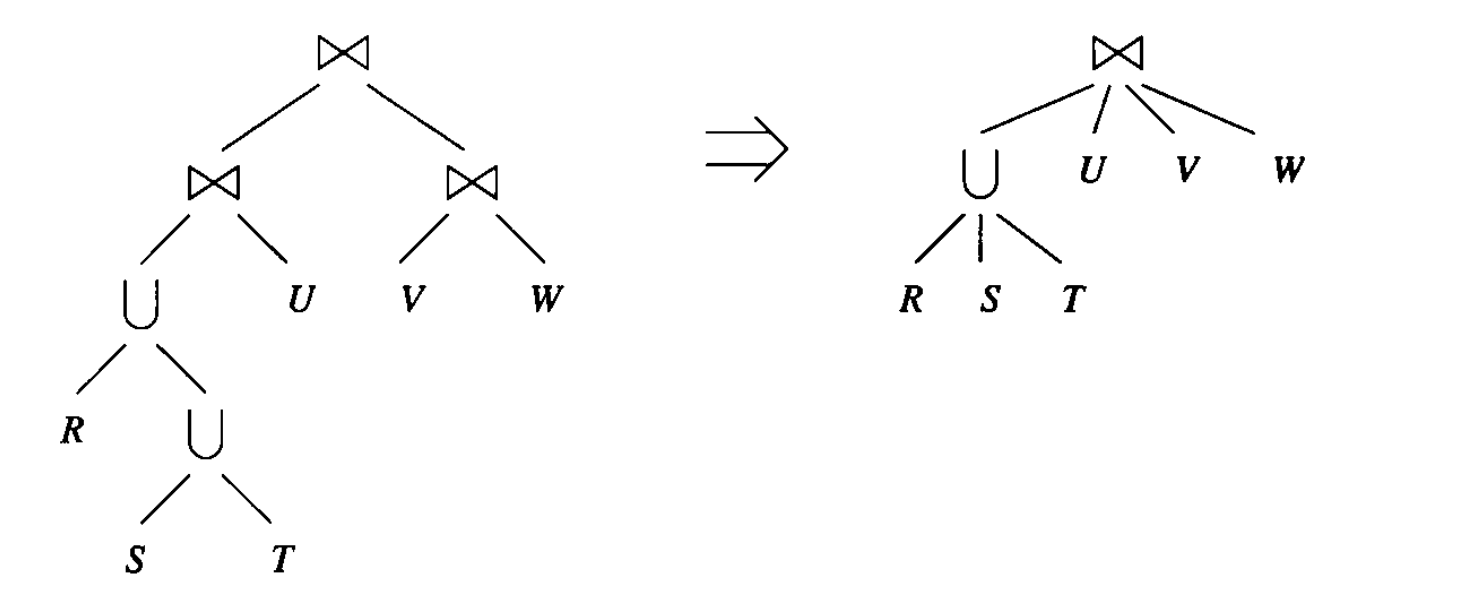
\includegraphics[width=0.8\linewidth]{handout/img/6-assoc-rule.png}
    \caption{可交换可结合的双目操作看成多目操作}\label{fig:6-assoc-rule}
\end{figure}

要确定夺目算子的计算顺序，优化的目标是使总的中间计算结果之和最小，可以使用动态规划来处理这个优化问题。一般是现在都采用贪婪算法，保证下一个的中间结果最小。

在分布式场景中，会假设内存足够大，通过MapReduce、Spark这样的分布式调度方案在各节点上传递数据，由于$\cap, \cup, \times, \bowtie$都支持tuple管道，分布式系统中处理这个问题的手法会不同。

\subsubsection*{左join树}

假设有$m$个关系组合成为一个多目操作，如果不加括号，多目算子的计算顺序等价于一个排列问题$m!$。双目操作的计算顺序落实到join树，有很多种如\figurename\ref{fig:6-join-tree}，其中最左join树对应于一个关系排列。

\begin{figure}[H]
    \centering
    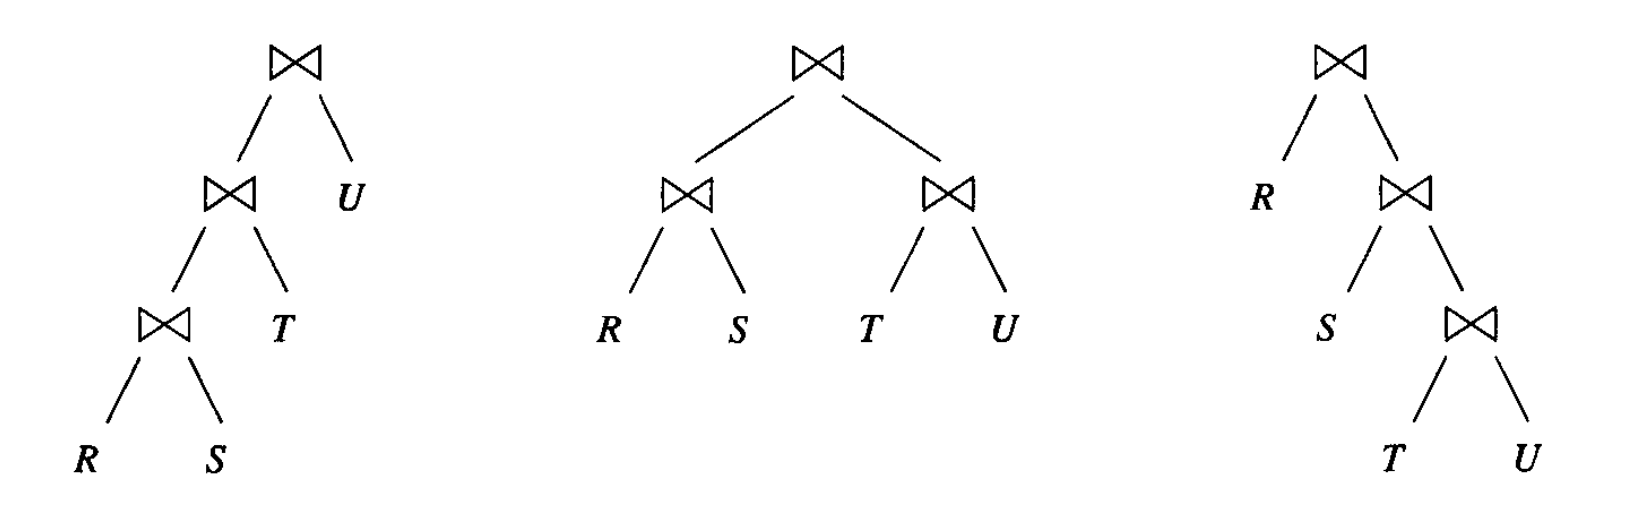
\includegraphics[width=0.8\linewidth]{handout/img/6-join-tree.png}
    \caption{join树}\label{fig:6-join-tree}
\end{figure}

在实现中，上一次$\bowtie$操作的结果不需要物化(merterialization)到磁盘，直接与选定的下一个关系做join操作。

\section{物理优化}

在完成逻辑优化后，得到一棵AST，最后一步是选择AST树上算子的实现算法，连接各算子。按照上一章的说法，算子连接主要有两种：tuple管道和物化。物理优化的主要工作是：1)~选择算子实现算法；2)~处理算子之间的连接。

根据上一章的讨论，主要关注的是$\times, \gamma, \tau, -, \bowtie, \bowtie_C$这些算子的输出，因为它们不支持单轮的tuple管道。具体的算子直接利用上一章的递推多轮算法。

物理优化仍然会在AST上标注，可以采用深度遍历方式处理，如\figurename\ref{fig:6-physical-plan}。

\begin{figure}[H]
    \centering
    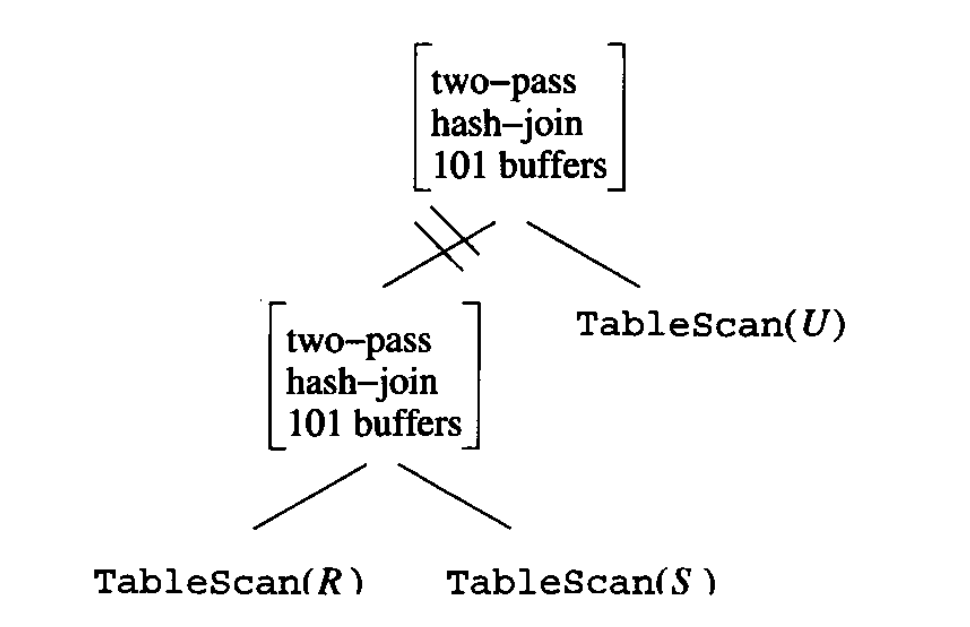
\includegraphics[width=0.6\linewidth]{handout/img/6-physical-plan.png}
    \caption{物理执行计划的树型表示}\label{fig:6-physical-plan}
\end{figure}
 % 6
\chapter{Concurrent}\label{chap:concurrent}

本章及后章介绍数据库系统的事务处理机制，主要包括事务并发与恢复两部分。

\section{Transaction}

数据库是数据的共享资源池，当多个用户同时访问数据库，必然会带来一致性方面的问题。事务是一个抽象概念，它将用户的多个操作原子化，要么全部执行要么全部不执行。Jim Gray在\cite{Gray1992Transaction}一书中对事务处理的方案做了完备的介绍，他将事务总结为ACID四个方面的特性：
\begin{itemize}
    \item 原子性：事务的执行是原子性的；
    \item 一致性：事务执行前后，数据库的状态保持一致；
    \item 隔离性：事务与事务之间是隔离的，彼此不会干扰；
    \item 持久性：事务一旦提交，其对数据库状态的改变是永久的；
\end{itemize}

事务的原子性并不是说事务执行有多快，它要求事务的执行效果要么完全发生，要么完全不发生。计算机组成原理中，CPU原子操作是指CPU指令在执行过程中不会被中断。事务的隔离性是指事务与事务之间是隔离的，即一个事务的执行不会影响到其他事务的执行。操作系统中，进程之间通过地址空间隔离，事务的隔离要求在并发控制下协调运行。

ACID四个特性中，最难理解的是一致性，这个一致性本质上是用户的要求，但数据库作为一个独立的系统，如何满足外部的要求，需知用户的要求是千变万化的。一致性有两方面的要求：在用户侧，要求事务执行前后，用户对数据库的修改能够保证状态的一致；在这个前提下，数据库系统承诺，事务在并发或者出错场景下，依然能保证按用户的要求执行或者不执行。

事务是一个抽象概念，在数据库系统上，它对应于用户执行BEGIN/COMMIT的一个操作序列，这个操作序列由数据系统的会话层执行，它会调用执行引擎在事务引擎的控制下推进，并将结果写入存储引擎，将过程记录在日志中。在事务的执行过程中，它会占用不同的资源，包括索引、页面、记录、元数据等等，在事务执行完毕后，这些资源被释放。

并非仅有数据库系统才提供事务服务。在一个复杂系统中：一个web服务器后台挂着一个数据库系统，暴露各种http服务，用户通过Restful API调用这些服务。当用户开启一个事务，概念上，事务并不仅仅是数据库系统的一个操作序列，它的操作包括从客户发出的请求，web服务器的响应动作，底层数据的执行序列，涉及的对象包括客户端、web服务器、数据库。微软曾经引入Jim改造自己的分布式系统框架ActiveCOM，目的是在各种业务系统上提供事务服务。

\begin{exercise}
    事务不仅仅存在与数据库中，文件系统同样存在着类似的概念，考查Journal文件系统的设计，仔细甄别文件系统对事务的需求，对比它与数据库事务的异同。
\end{exercise}
\begin{exercise}
    自云计算兴起后，数据广泛的存储在分布式节点上，分布式存储系统如何保持数据的一致性？
\end{exercise}

\section{事务模型}

为了便于讲述事务的并发与恢复，需要先对数据库事务的操作抽象，这些抽象并不能完全反映数据的所有操作，但对理解事务并发与恢复的机制足够了。

\subsection{行模型}

关系型数据的数据模型是关系，关系由元组组成，事务对关系的操作是对元组的增删改查。所谓行模型，是将对元组的操作抽象为read/write两个操作，显然行的读写模型并不能涵盖元组上的所有操作，读写操作要求是可逆的。读的可逆操作，就是简单的drop掉读到的数据，写的可逆操作要求取消写入的元组，当事务恢复时，在恢复中会要求撤销以前的写操作。

\begin{exercise}
    对一个关系的操作包括增删改查CRUD，这些操作的逆操作是怎样的？
\end{exercise}

\begin{figure}[H]
    \centering
    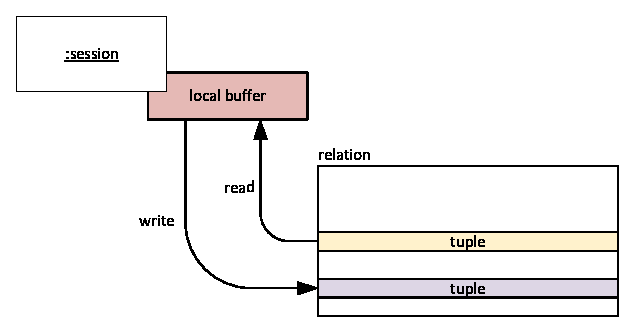
\includegraphics[width=0.8\linewidth]{handout/img/7-model.eps}
    \caption{行读写操作模型}\label{fig:7-model}
\end{figure}

\figurename\ref{fig:7-model}中，用户连接数据库，由会话代理用户执行SQL语句。假设一客户一会话，会话的本地缓冲对其它会话不可见。会话开启一个事务，先清空本地缓冲，然后按要求读元组，根据读到的元组在本地计算，最后将结果写入关系。写入关系的元组对其它事务不可见，只有当该事务提交后，事务的修改才可见。

有些事务实现不会在事务执行过程中去修改关系，而是在事务提交后，才去修改关系，这称为组提交策略。有些实现则在事务开启前不清空本地缓冲，这存在着风险，因为读到的数据可能不是最新，需要在修改元组或者提交事务时检查读到数据的有效性。在会话的实现中，除缓存元数据外，一般要求清晰地标定读集合与写集合，以便在提交事务时进行冲突检测。读集合与写集合除了保存元组数据外，还会保存元组的版本号。

会话代理执行SQL语句，不能假设事务的执行是线性的，事务的各种操作可能是并发的，例如一个事务可能会同时去读多个元组，或者一边读一边写。但在后文讲解中，一般都会假设事务的读写操作是顺序执行的，目的是为了便于表达，有助于理解事务的并发与恢复。总之，事务的行模型是一个读写操作的偏序模型，但讲解中用全序序列来表达。

$$
t=r(x)w(x)r(y)r(x)w(x)
$$

以上面的事务为例，事务先读$x$，然后写$x$，再读$y$和$x$，最后写$x$。这里例子里，事务对$x$元组写了两次，假设在事务可以在执行过程中写入关系，$x$对其它事务是不可见的；或者采用写提交策略，$x$的修改在会话本地，只有在事务提交后才会写入关系。后文在讨论事务并发中，一般会做如下假设，这个假设有助于简化讨论，并没有禁止事务实现对同一元组多次读写：

\begin{itemize}
    \item 在事务执行过程中，对同一元组不会读写两次；
    \item 在事务写入一个元组后，不会再读该元组；
\end{itemize}

行的读写操作一般由执行引擎实现，在并发控制中，锁方案要求控制对读写操作的推进，这要求并发控制会嵌入到执行引擎中。而在乐观并发控制中，读写操作的推进一般不受控制，事务在提交时会进行冲突检测。

\begin{exercise}
    如果采用偏序模型来描述事务执行的操作，它的表达应该是怎样的？
\end{exercise}
\begin{exercise}
    后文在介绍事务并发时，强加了不重复读写记录的假设。潜台词，事务的缺省隔离级别是多少？
\end{exercise}
\begin{exercise}
    在MVCC场景下，事务的执行是乐观的，在提交阶段才检查读写集合的冲突。我们前面假设会话执行SQL语句，会在本地保存记录的读集合与写集合，该如何实现？对比锁方案，能不能不在会话本地实现读写集合？
\end{exercise}

\subsection{树模型}

事务的操作抽象为行的读写，这种抽象是一种极致的简化，现实中，事务的操作远比行模型复杂得多。以一个银行转账事务为例，先从一个账户$a$提取1000元，然后将1000元存入另一个账户$b$。这两个操作要进一步分解为数据库的SQL语句，SQL语句然后被抽象为行的读写。

\begin{figure}[H]
    \centering
    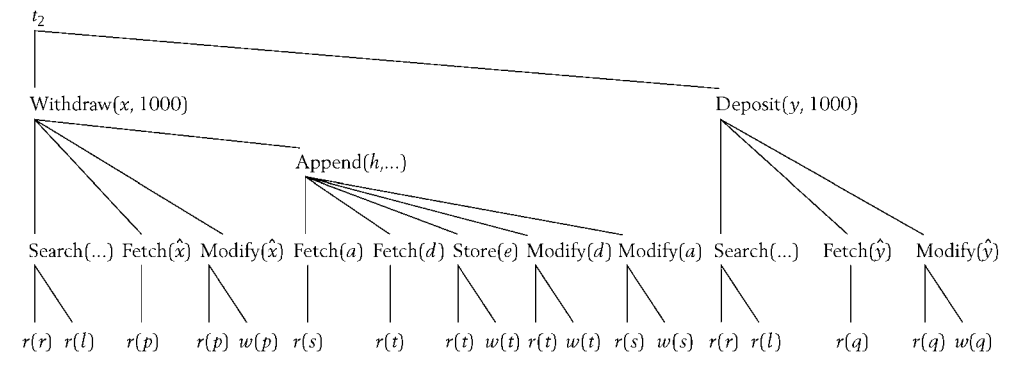
\includegraphics[width=\linewidth]{handout/img/7-tree.png}
    \caption{转账事务操作的树型模型}\label{fig:7-tree}
\end{figure}

在这个例子中，事务不仅是数据库上，而是全系统范围的操作序列。整个事务的执行被分解为多级，withdraw/deposit对应于账务的业务操作，Search/Fetch/Modify是数据库的操作，这些操作进一步分解为底层的行读写操作，所有操作按照树型组织。

树模型支持更丰富的语义，能够表达复杂的事务。树模型虽然分层，基础仍然是底层的行读写操作。以前面的withdraw为例，withdraw是一个业务操作，它会分解为数据库SQL语句，进一步分解为底层行模型。在业务层次，一般不会提供可逆操作，因为withdraw的分解并不一定是唯一的，withdraw的可逆性最终要依赖于底层的页模型来确保。

树模型的并发，也依赖底层页模型，底层页模型控制多个事务的推进。但是，并不是说树模型中某些操作不需要并发控制，有些中间操作是需要显式加入并发控制的。

数据库库内部的对象，并不仅限于数据元组，可能还有索引、页面、元数据等，在一个完整事务处理中，需要根据对象类型来处理并发与恢复，尤其是这些对象的逆操作实现。

\begin{exercise}
    一个聚集存储的页面上的操作有哪些？这些操作的逆操作如何实现？如果页面分裂，如何处理逆操作？
\end{exercise}
\begin{exercise}
    btree索引上的逆操作呢？
\end{exercise}

\subsection{版本模型}

将数据库存储的数据看成一个集合，每次事务提交对这个集合做更改。如果从用户需求来看，如果每次只访问最新的更新，整个数据集总是最新版本。这种模型下，事务并发一般采用锁方案，由两阶段锁2PL协议控制事务并发推进。锁方案下，事务更新的可见性按照标准分为4个隔离级别，这4种隔离级别的约束逐渐增高：

\begin{itemize}
    \item 读未提交（Read Uncommitted）：允许一个事务读取另一个事务未提交的数据，可能会导致脏读（Dirty Read），数据一致性差。
    \item 读已提交（Read Committed）：一个事务只能读取已提交事务的数据，避免了脏读，但可能会出现不可重复读（Non-repeatable Read）。
    \item 可重复读（Repeatable Read）：在同一事务中多次读取同一数据时，结果始终相同，避免了脏读和不可重复读，但可能会出现幻读（Phantom Read）。
    \item 可串行化（Serializable）：最高的隔离级别，强制事务串行执行，完全避免了脏读、不可重复读和幻读，但性能较低。
\end{itemize}

\begin{exercise}
    构造一个脏读的例子。
\end{exercise}
\begin{exercise}
    构造一个不可重复读的例子，在锁方案中，它出现的根本原因是什么？
\end{exercise}
\begin{exercise}
    构造一个幻读的例子，在锁方案中，它出现的根本原因是什么？
\end{exercise}

可串行化serializable与串行化serialized二者是存在根本区别的，可串行化目的是允许事务并发执行，串行化是将所有事务按照某种顺序串行执行。可串行化目的是提升系统吞吐量，执行的结果要等同于串行化执行，或者说，可串行化的目标是以并发的方式实现串行化的效果。

脏读、不可重复读、幻读的产生，都是由于是否加锁、是否加写锁、加读锁、对不存在项是否加锁的选择所致。要充分理解这4种隔离级别，需要从锁的方案出发。

如果用户允许数据库对象存在多个版本，但对象版本的增长要求为线性，此时可能会使得应用的性能得到显著提升。例如，一个公司要对上个月的销售情况做统计，这些统计操作并不需要最新的数据版本，允许读取一个历史版本即可。如果依赖于最新的数据，很可能会由于等待一个缓慢的事务，拖慢整个统计操作的完成时间。

\begin{figure}[H]
    \centering
    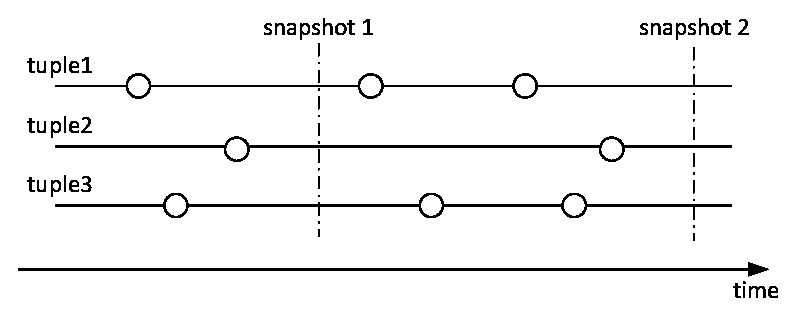
\includegraphics[width=0.8\linewidth]{handout/img/7-snapshot.eps}
    \caption{多版本事务}\label{fig:7-snapshot}
\end{figure}

如\figurename\ref{fig:7-snapshot}所示，每个元组有不同版本，根据时戳可以划分出不同的版本。对旧有版本的访问不会影响最新版本的更新，事务可以并发地读取不同版本的数据。

\begin{exercise}
    \figurename\ref{fig:7-snapshot}中展示的的多版本有统一的时钟，在分布式系统下，维护一个全局的物理时钟开销很大，如何利用因果关系在分布式节点上读取一个快照snapshot？参考\cite{lamport2019time}。
\end{exercise}

目前，数据库的多版本模型都是线性的，即对象可能存在多个版本，但是版本号是严格递增的。但有些应用中，版本的增加可能会出现分支，例如git版本控制系统。
\begin{exercise}
    线性版本系统，一般直接用时戳来标记版本。假设一个数据库的模板模型是非线性的，元组会出现分支版本，版本该如何表达？
\end{exercise}
\begin{exercise}
    假设有一个协同文档编辑系统，类似于wiki，它是一个非线性的版本系统吗？讨论一下。
\end{exercise}

\section{单版本并发}

在不同的版本模型下，事务并发控制的方案也不同。单版本模型下，事务读记录需要考虑该记录是否被修改或者将被修改，而多版本模型下，事务从某个snapshot上读数据，不会被阻塞。单版面模型需要考虑的资源共享问题更严格。

\begin{figure}[H]
    \centering
    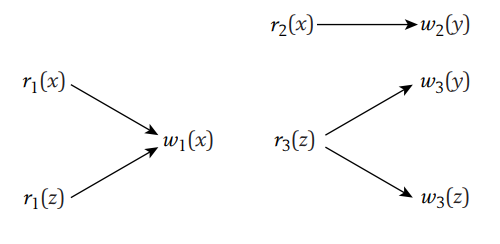
\includegraphics[width=0.6\linewidth]{handout/img/7-partial.png}
    \caption{三个事务}\label{fig:7-partial}
    \vspace{1em}
    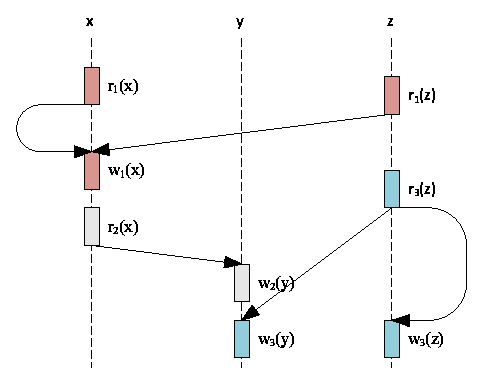
\includegraphics[width=0.7\linewidth]{handout/img/7-seq.eps}
    \caption{三个事务偏序执行}\label{fig:7-seq}
\end{figure}

\subsection{调度的正确性}

每个事务如果用偏序表达，多个事务并发，这些事务的r/w操作会交叠执行，将多个事务并发执行的偏序表达称为一个调度。在\figurename\ref{fig:7-partial}中有三个事务，它们的一种执行顺序如\figurename\ref{fig:7-seq}所示。我们要判定\figurename\ref{fig:7-seq}的执行过程是否符合事务的一致性要求，如果符合，这三个事务的并行执行就是合法的。

根据ACID的原则，一致性要求一个事务$t$执行前后数据库的状态必须是一致的。数据库的状态一致，在不同的场景下语义可能不同，行的读写操作并不能保证一致性，这种一致性是由用户保证的，数据库无法做出承诺。回到\figurename\ref{fig:7-partial}，可以断定单独执行$t_1, t_2, t_3$，数据库的状态是一致的，并且串行执行$t_1, t_2, t_3$三个事务，最终结果也是一致的。由此，判定\figurename\ref{fig:7-seq}是否合法，就需判定它是否等价于某个串行执行的结果。

\begin{exercise}
    假设有$n$个事务，它们串行执行的方案有多少种？
\end{exercise}
\begin{exercise}
    如果多个事务偏序并发，它们的并发方式比串行执行更多吗？是否每种偏序并发会对应于一种串行执行的结果？
\end{exercise}

\figurename\ref{fig:7-seq}的执行结果实际上等价于$t_1 > t_2 > t_3$，$r_3(z)$虽然在$t_2$前执行，但$z$的值与$t_2$是无关的，即使$r_3(z)$向下滑动到$w_2(y)$之后，结果仍然是相同的。

\begin{exercise}
    \figurename\ref{fig:7-seq}中，$w_3(z)$向上滑动到$w_2(y)$之前，是否是一致的？对数据库而言是一致的，但是数据库作为一个系统，它要向外暴露内部状态，在外部看来，$y,z$的数据更新发生交叠，这并不符合一致性预期。在单节点服务器上，要求事务的提交是顺序的，分布式数据库呢，是否也要求事务提交的全局顺序性？
\end{exercise}
\begin{exercise}
    \figurename\ref{fig:7-seq}中，如果将$w_2(y), w_3(y)$位置交换，是否是一致的？$w_1(x), r_2(x)$交换呢？
\end{exercise}

\subsection{调度的可串行化}

调度的可串行化serializable，是指一个调度等价于某个串行执行的结果。按照\cite{Weikum2001Transactional}，有多种等价定义，如语义可串行化、结果可串行化、视图可串行化、冲突可串行化等。其中，语义可串行化计算调度的语义，但如前所述，语义的定义与特定应用相关，数据库无法单独定义。结果可串行化只看调度完成后是否与某个串行调度等价，未考虑并发过程。视图可串行化VSR在结果可串行化的基础上，约束并发执行每一个操作都等价于某个串行调度，由于串行调度的数量庞大，是个NP难题。本文只从冲突可串行化开始介绍，更多的可串行化定义参考\cite{Weikum2001Transactional}。

\subsubsection*{冲突}

非形式化的，冲突是指同一资源上，两个事务间的操作间的关系。考虑行模型，记录上只有两种操作：读取和写入。$t_1$事务对资源$x$写入$w_1(x)$，$t_2$事务对资源$x$读取$r_2(x)$，如果$w_1(x)$在$r_2(x)$之前执行，$t_1$和$t_2$是冲突的。行模型中，只有$r_1(x)r_2(x)$操作是不冲突的，其余写操作都会引起冲突。

冲突发生，实际上规定了事务间的执行顺序，以$w_1(x)r_2(x)$为例，它要求$t_1 > t_2$。利用从冲突得到的事务间偏序关系，可以构造后面的冲突图，如果图上存在环，则可以判定调度不可串行化，这是引入冲突概念的目的。

给定一个调度$s$，找出在同一资源上的所有两两冲突关系，这些两两冲突构成了这个调度的冲突集，利用这个冲突集可以构造后文的冲突图。当两个调度的冲突集相同，称这两个调度等价。
$$
s=w_1(x)r_2(x)w_2(y)r_1(y)w_1(y)w_3(x)w_3(y)c_1a_2
$$
上式中，调度$s$的冲突集如下。在计算冲突集时，当遇到取消事务时，简单地将该事务的所有操作忽略掉，例如上式中$t_2$被取消，$r_2(x)$和$w_2(y)$都被忽略。
$$
conf(s) = \{ (w_1(x),w_3(x)), (r_1(y), w_3(y)), (w_1(y), w_3(y)) \}
$$

\begin{exercise}
    两个调度$s, s'$是否等价？
    $$
    s=r_1(x)r_1(y)w_2(x)w_1(y)r_2(z)w_1(x)w_2(y)
    $$
    $$
    s'=r_1(y)r_1(x)w_1(y)w_2(x)w_1(x)r_2(z)w_2(y)
    $$
\end{exercise}

\subsubsection*{冲突可串行化CSR}

按照可串行化正确性的规定，冲突可串行化定义为：如果一个调度与某个串行调度等价，称这个调度是冲突可串行化的。举例而言，
$$
r_1(x)r_2(x)r_1(z)w_1(x)w_2(y)r_3(z)w_3(y)c_1c_2w_3(z)c_3
$$
上式的冲突集为
$$
\{ (r_2(x), w_1(x)), (w_2(y), w_3(y)), (r_1(z),w_3(z))\}
$$
这个冲突集等价于$t_2 < t_1 < t_3$，如果刨除调度尾部的提交动作，这个调度是冲突可串行化的。注意到上式中提交顺序$c_1c_2c_3$与等价串行化序列并不相符，后文将定义更严格的提交保序冲突可串行化。

再举一个例子，$r_2(y)w_1(y)w_1(x)c_1w_2(x)c_2$的冲突集为$\{(r_2(y),w_1(y)),(w_1(x),w_2(x))\}$，冲突集的两项是矛盾的，没有串行化序列与之对应。从这个例子，进一步引申出冲突图的概念，冲突图是一个有向图，图中每个节点对应于一个节点，冲突关系规定了两个节点的先后顺序，从前一个节点指向后一个几点。要判定一个调度是否合法，只需保证冲突图无环。

\begin{figure}[H]
    \centering
    \begin{tikzpicture}[node distance=4cm, auto, >=stealth]
        % 事务节点
        \node[draw, circle, minimum size=0.8cm] (t1) {$t_1$};
        \node[draw, circle, minimum size=0.8cm, right of=t1] (t2) {$t_2$};

        % 冲突边
        \draw[->, thick] (t2) to [bend left=30] node[above] {$r_2(y), w_1(y)$} (t1);
        \draw[->, thick] (t1) to [bend left=30] node[below] {$w_1(x), w_2(x)$} (t2);
    \end{tikzpicture}
    \caption{冲突集$\{(r_2(y),w_1(y)),(w_1(x),w_2(x))\}$对应的冲突图}
    \label{fig:conflict-graph}
\end{figure}

\subsubsection*{提交保序可串行化COP}

冲突可串行化CSR没有考虑到提交顺序，提交顺序保持冲突可串行化Commit-Order Preserving CSR(COP)在CSR基础上，要求提交顺序与CSR串行化顺序一致。
$$
s_1 = w_1(x)r_2(x)c_2w_3(y)c_3w_1(y)c_1
$$
$s_1$是CSR，等价串行化调度为$t_3t_1t_2$，按照COP定义，事务提交顺序是$t_2t_3t_1$。

$$
s_2 = w_3(y)c_3w_1(x)r_2(x)w_1(y)c_1c_2
$$
$s_2$是CSR，等价串行化调度为$t_3t_1t_2$。提交顺序是$c_3c_2c_1$，$s_2$是COP。

\begin{figure}[H]
    \centering
    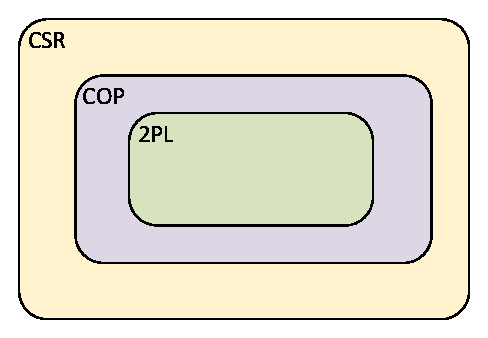
\includegraphics[width=0.4\linewidth]{handout/img/7-cop.eps}
    \caption{CSR、COP、2PL间的关系}\label{fig:7-cop}
\end{figure}

\begin{exercise}
计算下式的冲突集，等价串行化调度，画出冲突图，是否COP。
$$
s = r_1(y)r_3(w)r_2(y)w_1(y)w_1(x)w_2(x)w_2(z)w_3(x)c_1c_2
$$
\end{exercise}

\subsection{锁方案}

COP是大多数基于锁方案的事务并发的理论基础。冲突发生，实际上规定了两个事务间的先后顺序，确定了CSR对应的串行化调度，当提交顺序与CSR串行化顺序一致时，调度就是COP。事务提交顺序与CSR串行化顺序不一致，会破坏事务的可见性。但事务何时提交完全由用户确定，事务引擎实现只能退而求其次，禁止所有冲突的发生。也就是说，事务访问资源，如果发生冲突，会阻止事务推进，阻塞事务，这种机制正好用锁来实现。

\begin{exercise}
    冲突可串行化的接受调度为COP，由于不确定事务间的提交顺序，只能采用锁方案。锁方案采用后文的2PL协议，接受的调度集合是COP的子集。假设已知事务及其提交顺序，有没有可能实现COP？
\end{exercise}

回顾一下事务并发的场景，会话代理执行SQL语句，这些语句会读写底层记录。为了尽可能提升系统吞吐量，系统需要支持多事务并发。采用锁来实现冲突检测，当事务访问资源，检测是否发生冲突，如果发生冲突，阻塞事务执行，等待其他事务释放锁。当其它事务提交，是否资源上的锁，锁会通知事务线程继续执行。

事务的推进由锁控制，它的逻辑是嵌入到行模型的读写操作中，这不太友好，好消息是树模型的事务虽然复杂，我们只需要关注底层行模型的实现即可。

\subsubsection*{事务状态机}

在数据库中，会话代理用户执行SQL语句，一个会话对应一个客户。会话是活动对象，通常用线程或者进程来表示。当会话开启一个事务，事务进入Running状态，访问资源发生冲突，事务被阻塞。事务完成后，进入提交状态，这是事务的终态。当事务被取消，事务会重启，重新开始，如\figurename\ref{fig:7-states}。

\begin{figure}[H]
    \centering
    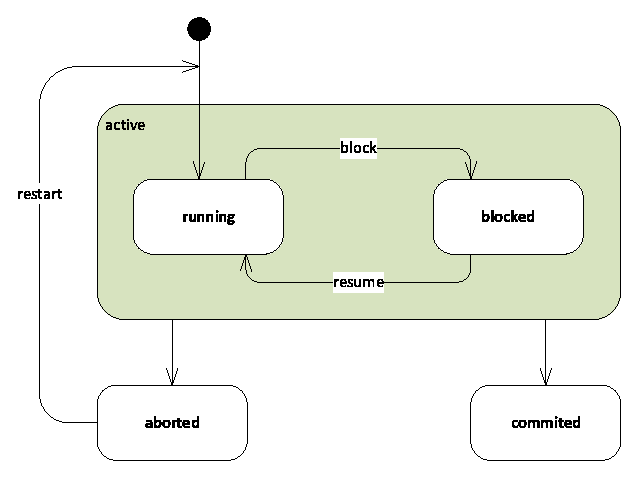
\includegraphics[width=0.8\linewidth]{handout/img/7-states.eps}
    \caption{事务状态机}\label{fig:7-states}
\end{figure}

\subsubsection*{锁表}

锁方案在内存中建立一个锁表，每行对应于一把锁。当事务访问记录时，在锁表中创建记录对应的锁，然后对记录加读锁或写锁。如果加锁成功，事务继续执行；如果加锁失败，事务阻塞，等待其他事务释放锁。

\begin{exercise}
    锁方案中，一条记录一把锁，可以在记录上建立锁吗？
\end{exercise}

由于行数会很多，而事务访问的资源，在某些场景下并不一定很多，所以锁表里的锁是按需创建的。但在记录中内嵌锁，并不是不可行，只是在传统关系型数据库中，系统崩溃，意味着接受的未完成事务会被放弃，持久化锁没有意义。而在分布式系统中，系统运行的容错模型要求$7 \times 24$不间断，单个节点崩溃意味着锁的丢失，其余节点重启服务，会导致事务推进错误，所以在Percolator\cite{peng2010large}中锁被持久化到kv存储中。

锁表包含锁，事务访问资源，会先进入锁表查看资源是否有锁，如果没有则创建，然后加锁。如果有锁，则访问该锁。目前的锁表方案是hash+btree，利用hash实现对点加锁，利用btree处理范围锁。

\begin{exercise}
    能否利用区间树interval tree来设计锁表，支持点、范围加锁？
\end{exercise}

\subsubsection*{锁的设计}

锁的基本结构，如\ref{fig:7-lock}所示，每个记录对应于一把锁，锁的状态包括未加锁、读锁、写锁。当事务访问记录时，在锁表中创建记录对应的锁，然后对记录加读锁或写锁。如果加锁成功，事务继续执行；如果加锁失败，事务阻塞，进入等待状态，等待其他事务释放锁。

\begin{figure}[H]
    \centering
    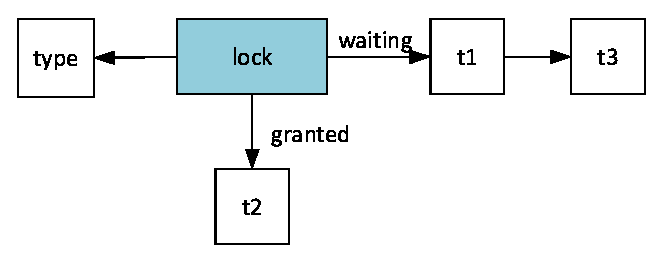
\includegraphics[width=0.6\linewidth]{handout/img/7-lock.eps}
    \caption{锁的设计}\label{fig:7-lock}
\end{figure}

将读锁标记为S，写锁标记为X，根据冲突检测规则，S锁与S锁不冲突，S锁与X锁冲突，X锁与X锁冲突，有\figurename\ref{fig:7-lock}的相容性矩阵。

\begin{table}[H]
    \centering
    \caption{S锁和X锁的相容性矩阵}\label{tab:lock}
    \begin{tabular}{ccc}
        \toprule
        \textbf{请求类型} & \textbf{已加S锁} & \textbf{已加X锁} \\
        \midrule
        \textbf{S锁} & $\checkmark$ & $\times$ \\
        \textbf{X锁} & $\times$ & $\times$ \\
        \bottomrule
    \end{tabular}
\end{table}

事务在执行过程中，开始可能并不知道是否要对一行加锁，后面才决定写该行。此时事务持有S锁，如果没有其它事务同时持有这个S锁，可以安全地升级为X锁。这里的问题是，如果该S锁被多个事务持有，升级为X锁会导致其他事务阻塞，该如何处理？一般的方案是，将该锁标记为待升级，待升级标志指向希望升级的事务。进一步，当多个持有S锁的事务同时希望升级，会发生死锁。

行模型是一种简单的模型，数据库中除了行外，还包括索引、页等结构，事务对这些结构的访问，要复杂一些。以SELECT FROM WHERE语句为例，事务需要先查询btree索引，找到符合条件的记录，然后对这些记录加S锁。多数数据库实现中，将btree看成是内部数据结构，以latch方式加锁，latch不同于lock，它用完后立即释放。innodb实现中，先对btree加latch，找到记录后，对记录加S锁，释放latch，latch不遵循后面的2PL协议。考虑到事务正在读该表的某行，innodb可能会对该表加一个意向锁，禁止删除该表。

从上面的讨论中，可以看到，数据库中锁的设计非常精妙细微，一般分为表锁和行锁，表锁的设计需要根据细微的语义设计兼容性矩阵。

\begin{exercise}
    检查innodb与PostgreSQL中表锁的设计，体会这些锁的设计意图。
\end{exercise}

\subsubsection*{2PL协议}

事务对资源的访问一般遵循两阶段2PL协议，获取锁后，事务会持续访问资源，直到提交或回滚。2PL协议是说事务对锁的持有和释放是有序的，先获取锁然后再释放，观察\figurename\ref{fig:7-2pl}，事务的资源持有呈现为单峰。注意，单峰的衰减实际发生在提交或回滚阶段，设想一下，如果在提交前释放锁，意味着放弃对该资源的冲突检测。

采用2PL协议实现的调度器，它接受的调度集合是COP的子集，如\figurename\ref{fig:7-cop}。

\begin{figure}[H]
    \centering
    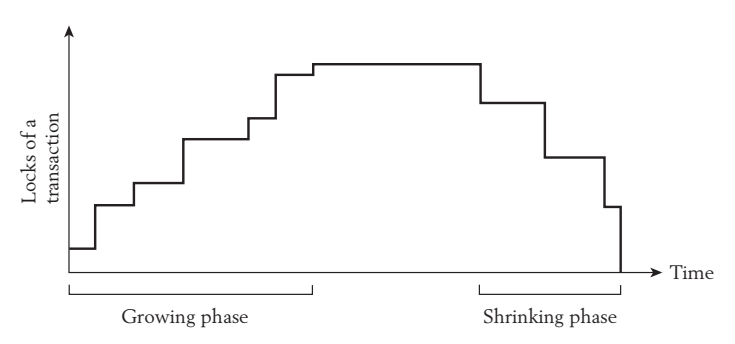
\includegraphics[width=0.8\linewidth]{handout/img/7-2pl.png}
    \caption{2PL协议}\label{fig:7-2pl}
\end{figure}

\begin{exercise}
    在2PL协议中，在提交前先释放读锁是否可行？如果不可行，举出反例。
\end{exercise}

\subsubsection*{死锁检测}

数据库内部加表锁和行锁后，可能会导致死锁的发生，死锁是多个事务彼此持有资源，等待对方释放锁，导致所有事务无法推进。操作系统课程中，关于死锁部分的内容包括死锁的检测和避免。数据库中采用类似的方案，一般会维护一个全局等待图。

在等待图waiting graph中，每个事务对应于一个节点v，当事务$t_1$等待某个锁，该锁被其它事务$t_2$持有，会画一条边$t_1 \rightarrow t_2$，从$t_1$出发，沿着这些边遍历，如果形成环，则表面存在死锁，对应着资源的彼此持有。实现中，这个等待图比较大，一般是在事务阻塞时启动一个定时器，超时后从该事务出发检测死锁。

当检测到死锁，会以某个标准选出环上的一个事务来牺牲，打破等待环，被选中的事务回滚重试。

\begin{exercise}
    事务由会话发起，构思一下这个等待图如何设计与实现。每个节点用vector容纳出边，对应于一个会话，会话有指针指向这个vector，出边需要描述lock。然后带入前述的多事务升级共享锁导致的死锁，看看这个方案需要补充什么。
\end{exercise}

\subsubsection*{死锁预防}

目前的死锁预防策略主要是基于时戳，假设每个事务启动都带有一个初始时戳，在此前提下，有如下两种方案：
\begin{itemize}
    \item wait-die：一个事务请求锁时，如果锁被其它事务持有，且该事务的时戳较大，那么该事务会等待；如果锁被其它事务持有，且该事务的时戳较小，那么该事务会回滚。也就是说，事务只会等待更年轻的事务，否则会回滚。
    \item wound-wait：一个事务请求锁时，如果锁被其它事务持有，且该事务的时戳较小，那么该事务会等待；如果锁被其它事务持有，且该事务的时戳较大，那么该事务会尝试杀死持有该锁的事务。也就是说，事务只会等待更老的事务，否则会杀死年轻事务。
\end{itemize}

现代主流数据库较少采用死锁预防，而更倾向于死锁检测，原因是死锁预防方案会减少可接受的调度集合，而死锁检测方案不会。

\section{多版本并发}

这本讲义中，关于锁的内容主要参考了\cite{Weikum2001Transactional}，可惜的是，mvcc方案真正成熟是在2009年之后。TIS\cite{Weikum2001Transactional}对多版本并发的描述较为简略，并且个人认为这部分的理论分析是错误的。

本节的内容主要参考了\cite{berenson1995critique, fekete2005making, cahill2009serializable}。\cite{berenson1995critique}指出SQL-92标准中的4种隔离级别用几种异常来划分，并不能正确区分一些某些异常，并提出一种基于多版本的snapshot isolation隔离级别。\cite{fekete2005making}形式化定义了 SI 的语义模型，指出write-skew是 SI 的根本缺陷。\cite{cahill2009serializable}在SI基础上，自动检查并阻断写偏序write-skew异常的发生，从而实现可串行化。

\subsection{一些基本前提}

在讨论多版本并发前，需要明确一些基本前提。多版本事务模型是线性的，对象按照线性版本递增。每个事务都带有两个时戳，一个是启动时戳，一个是提交时戳\cite{berenson1995critique}，一般用启动时戳来标记事务。启动时戳是事务执行BEGIN语句分配的时戳，提交时戳是事务执行COMMIT语句分配的时戳，时戳的分配是全局递增的，这在分布式场景下要求过于严格。

\begin{exercise}
    查阅google spanner的论文，了解truetime的设计目标与方案。
\end{exercise}

事务使用启动时戳读取数据，在会话本地计算，本地缓冲临时版本，使用组提交策略，这避免了脏读。事务执行COMMIT命令，先用latch锁住所有写入对象，然后用会话局部版本更新数据，提交后释放latch。

\begin{exercise}
    不用latch用锁行不行？可以的，这里用latch主要是因为SI隔离级别实现是无锁的。在\cite{cahill2009serializable}中，SSI可串行化的调度器使用了锁，参考一下该论文。
\end{exercise}

事务读取的版本是启动时戳之前的最近版本，启动时戳实际上对应了一个快照snapshot，加上组提交策略，事务天然避免了脏读和不可重复读，这对应了一个称为snapshot isolation的隔离级别\cite{berenson1995critique}。SI隔离级别并不等同于可重复读隔离级别，因为它并没有杜绝幻读，同时具有写偏write-skew异常。不能说SI与RR隔离级别哪个更高，基于锁的RR隔离级别与SI不完全等同。

\begin{exercise}
    参考一下\cite{berenson1995critique}，指出SI隔离级别与RR隔离级别为什么不同。
\end{exercise}

mvcc讨论的基线是SI隔离级别，因为SI基本非常吸引人，它天然高于读未提交RU和读已提交RC隔离级别，并且没有在对象上加锁，这使得它具有更好的性能。

\subsection{SI}

SI隔离级别的实现非常容易，事务读取启动时戳的快照，在提交时刻检查是否存在被提交时戳更高的版本即可。多个事务同时提交，latch竞争采用first-write-wins策略，即先提交的事务获得latch，后提交的事务等待。

\begin{figure}[H]
    \centering
    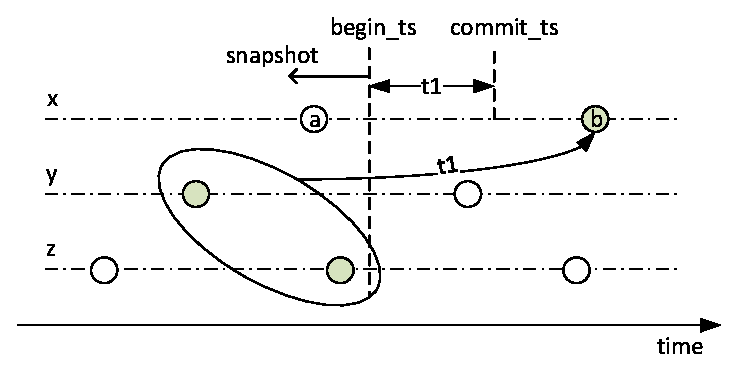
\includegraphics[width=0.8\linewidth]{handout/img/7-version.eps}
    \caption{提交写入过程}\label{fig:7-version}
\end{figure}

这里需要对提交时戳做一个更细部的说明，如\figurename\ref{fig:7-version}，事务读取启动时戳快照上的版本$y, z$，然后更新$x$。采用组提交策略，写入$x_b$版本时，使用提交时戳。事务的提交是需要时间的，对$x$的写入并不会发生在提交时戳的当下，而是需要拖后一段时间。如果latch加锁不成功，还可能导致事务的回滚。

\begin{exercise}
    mvcc中，是否需要检查死锁？如何防止latch的死锁？
\end{exercise}

\subsection{版本冲突}

令人惊讶的是，mvcc的相关理论与技术在2009年前后才成熟，而其时已进入了云计算与大数据时代。在此之前，Oracle 9.2宣称的SERIALIABLE隔离级别，实际上是SI隔离级别\cite{fekete2005making}。

与单版本并发类似，多版本并发的正确性准则仍然是——并发调度是否等价于多个事务的串行化调度。单版本上要求冲突集等价，多版本上仍然是要求冲突集等价，但是多版本上的冲突定义有变化，甚至可以不称之为冲突。单版本的冲突表现为同一行上操作间不相容，一个事务在改变数据，另一个事务依赖于旧值。而在多版本上，读写分别落在不同的版本上，写不会改变旧值，新版本的增加带来的问题更多的要从因果逻辑上看。

下面分析多版本的冲突，设有一个对象$x$，它的版本为$x_1, x_2, x_3, \ldots$，每个版本都有一个时戳$t_1, t_2, t_3, \ldots$。在讨论冲突时，需要讨论相邻版本间的冲突，即$x_1$与$x_2$、$x_2$与$x_3$等版本之间的冲突。跨版本间不存在冲突，例如$x_1$与$x_3$之间不存在冲突。同时，不同数据$x,y$上的操作间不存在冲突。

\subsubsection*{rr}

虽然由于两个事务$t_1, t_2$的启动时戳不同，对应于不同的快照，两个事务读同一个版本的对象，并不冲突。如\figurename\ref{fig:7-rr1}，两个事务启动时戳不同，对应于不同的快照，但读同一个版本的$x$，它们并不冲突。由于没有冲突，我们无法根据对该版本的读操作推测两个事务的串行化先后顺序。

对于读操作而言，无需讨论两个事务读不同版本的情况，如$r_1(x_1)r_2(x_2)$。原因在于，事务读到的版本不同，必然有某个事务写入了新版本，本质上是读写rw/wr关系，而不是不同版本的读读关系。

\begin{figure}[H]
    \centering
    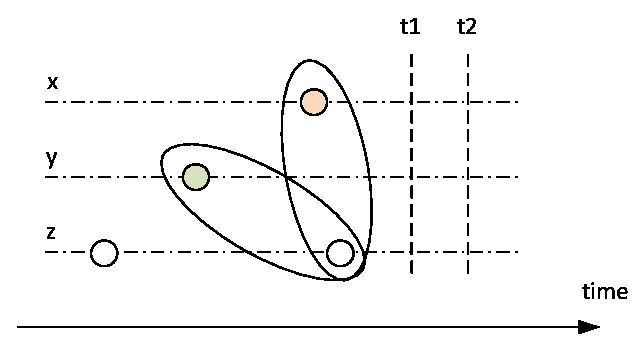
\includegraphics[width=0.6\linewidth]{handout/img/7-rr1.eps}
    \caption{两个事务读同一版本}\label{fig:7-rr1}
\end{figure}

在\figurename\ref{fig:7-rr2}中，事务$t_1$读取$x_a$，事务$t_2$读取$x_b$，但在$t_2$之前一定有一个$t_3$事务写入了$x_b$版本。

\begin{figure}[H]
    \centering
    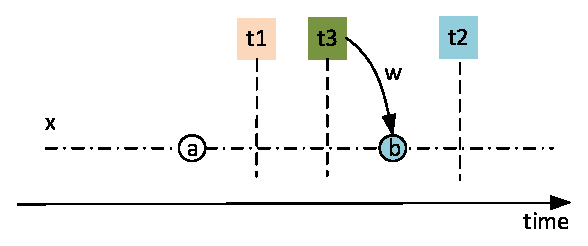
\includegraphics[width=0.6\linewidth]{handout/img/7-rr2.eps}
    \caption{两个事务读不同版本}\label{fig:7-rr2}
\end{figure}

\subsubsection*{wr}

一个事务写入新版本，另一个事务读取该版本，$w_1(x_1)r_2(x_1)$，两个事务操作在同一版本上。考查这种wr关系，它规定了写事务必须先写入，才能被读事务读取。

\begin{figure}[H]
    \centering
    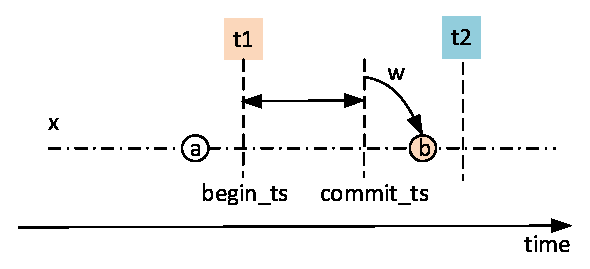
\includegraphics[width=0.6\linewidth]{handout/img/7-wr.eps}
    \caption{写读wr冲突}\label{fig:7-wr}
\end{figure}

在组提交策略下，$w_1(x)$写入动作在提交前做出，意味着$t_1$的提交时戳必然小于$t_2$的启动时戳，否则$w_1(x)$对$t_2$不可见，如\figurename\ref{fig:7-wr}。因此wr冲突的两个事务不会其实不会出现并发执行，$t_1, t_2$本身是串行执行的，在后文中wr不被认为是一种冲突。由于采用组提交策略，在表示调度时，一个事务写入新版本，后面会紧跟着提交动作。

\subsubsection*{rw}

一个事务读取老版本，另一个事务写入新版本，$r_1(x_0)w_2(x_2)$。两个事务操作在不同版本上，这是一个读写冲突，如\figurename\ref{fig:7-rw}。
\begin{figure}[H]
    \centering
    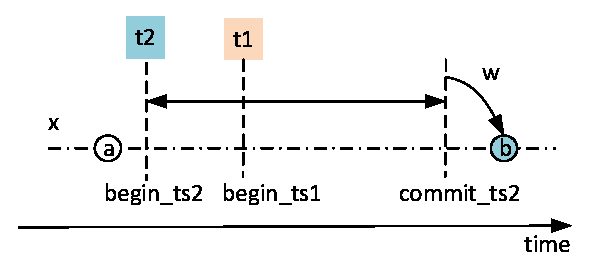
\includegraphics[width=0.6\linewidth]{handout/img/7-rw.eps}
    \caption{读写rw冲突}\label{fig:7-rw}
\end{figure}

在\figurename\ref{fig:7-rw}中，$t_2$写入版本$x_b$，$t_1$读取版本$x_a$，$x_b$对$t_1$不可见，说明begin\_ts1 < commit\_ts2。

对rw的分析可以有两种方法，一种是观察并发是否相对于串行化调度引入了新的冲突，另一种是根据rw的冲突含义，分析是否会产生因果矛盾。

将一个事务看成一个函数，读取作为输入，写入作为输出，输出依赖于输入。这个假设中，可能某个输出只依赖于部分输入，但这是用户所知，作为数据库而言，只能假设一个输出依赖于所有输入。

将事务的所有读取行记作读集合rset，事务的所有写入行记作wset。\figurename\ref{fig:7-rw}中的读写冲突实际上是两个事务的读写集合出现了版本交叠，如\figurename\ref{fig:7-wset}所示。

\begin{figure}[H]
    \centering
    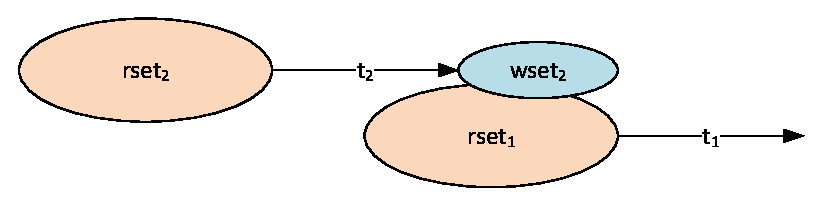
\includegraphics[width=0.8\linewidth]{handout/img/7-wset.eps}
    \caption{两个事务读写集合交叠}\label{fig:7-wset}
\end{figure}

$r_1(x_0)w_2(x_2)$这两个作用在$x$对象上的操作本身并不冲突，它们是两个版本。但问题是每个事务从rset $\rightarrow$ wset，这是一个因果关系，两个事务在这个前提下有可能会产生因果矛盾。


两个事务的等价串行化调度为$t_1t_2$或者$t_2t_1$，rw冲突下有$rset_1 \cap wset_2 \neq \emptyset$，先考查$t_1t_2$串行化调度，然后考查$t_2t_1$串行化调度：

\begin{itemize}
    \item $t_1t_2$：
    \begin{itemize}
        \item \figurename\ref{fig:7-rw2}中(a)所示，$t_1$先执行$t_2$后执行，冲突集中可能会包含一些wr冲突，但冲突并不意味着不可串行化。
        \item 将$t_1$向右滑动，如果$wset_1 \cap rset_2 = \emptyset$，冲突集没有变化，但不能就此判断是否可串行化。因为$t_1$的wset有可能与其它事务的rset交叠，导致新的冲突。
        \item \figurename\ref{fig:7-rw2}中(b)所示，如果$wset_1 \cap rset_2 \neq \emptyset$，并且$wset_1$对$t_2$不可见，这里有新的冲突$r_2(y_0)w_1(y_1)$。逻辑上，$t_2$的输出部分依赖于$t_1$，$t_1$的输出部分依赖于$t_2$，而(b)中这些输出又相互不可见，是矛盾的。
        \item 当$t_1$继续向右滑动，需要考虑$wset_1 \cap wset_2$，这是ww冲突。
    \end{itemize}
\end{itemize}

\begin{figure}[H]
    \centering
    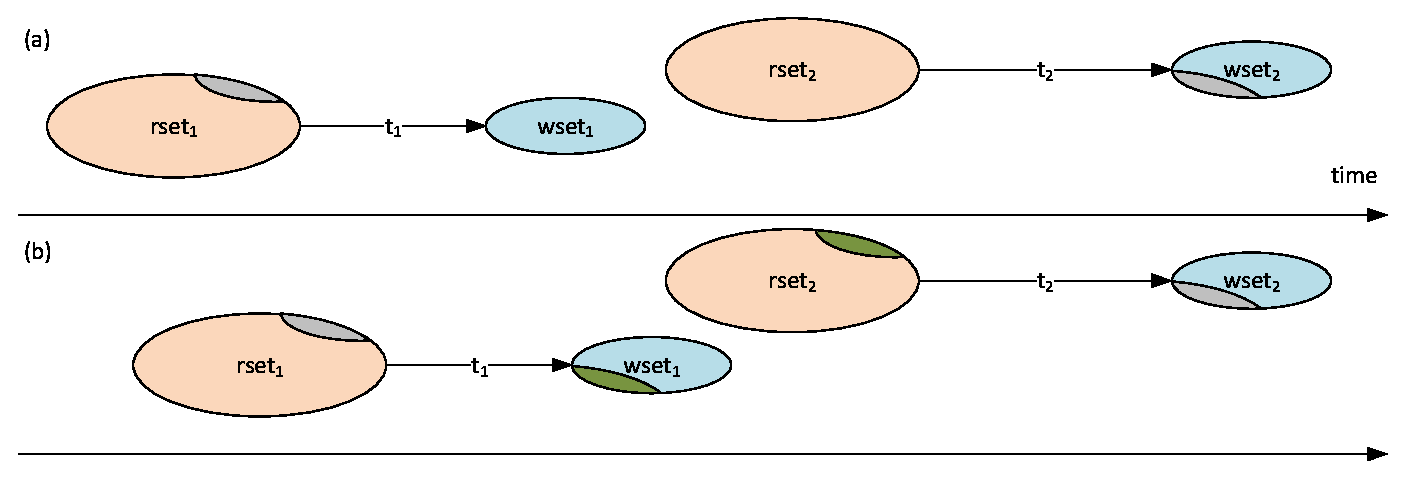
\includegraphics[width=\linewidth]{handout/img/7-rw2.eps}
    \caption{rw等价于$t_1t_2$冲突集}\label{fig:7-rw2}
\end{figure}

\begin{exercise}
    考查$t_2t_1$的等价冲突集。
\end{exercise}

rw读旧版本写新版本，两个事务分别在两个版本上操作，这两个操作之间其实没有冲突，关键是按照因果关系，事务间可能因为rset与wset之间的交集形成彼此依赖的循环关系。

\subsubsection*{ww}

两个事务写同一个对象，$w_1(x_1)w_2(x_2)$，这两个事务操作在不同版本上，两个操作本身没有冲突。在\figurename\ref{fig:7-ww}中，$t_1$先执行$t_2$后执行，冲突集中可能会包含一些ww冲突。在后文分析中，ww之间存在的问题实际上被转化为rw冲突。

\begin{figure}[H]
    \centering
    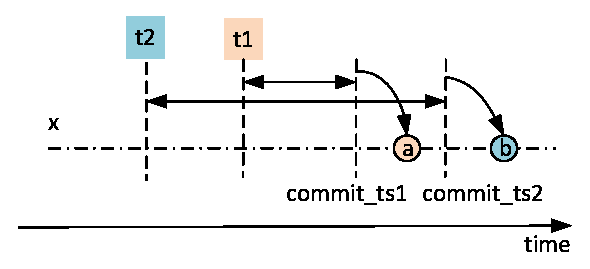
\includegraphics[width=0.6\linewidth]{handout/img/7-ww.eps}
    \caption{写写ww冲突}\label{fig:7-ww}
\end{figure}

两个事务$t_1, t_2$的等价冲突集，如\figurename\ref{fig:7-ww2}所示，在(b)中，假设$rset_1 \cap rset_2 \cap wset_1 \cap wset_2\neq \emptyset$，$t_1, t_2$读取相同的对象，会引入新的冲突rw。本讲义中，ww不被认为是一种冲突，因为它最终会转化为rw冲突，只需要在提交时刻保证新写入的版本时戳更高即可。

\begin{figure}[H]
    \centering
    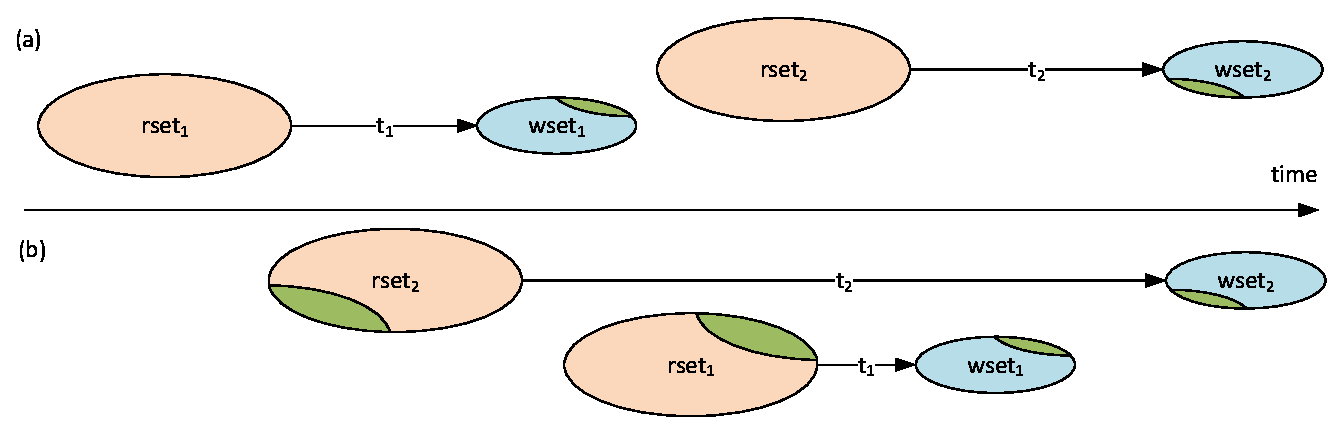
\includegraphics[width=\linewidth]{handout/img/7-ww2.eps}
    \caption{ww等价于$t_1t_2$冲突集}\label{fig:7-ww2}
\end{figure}

根据前面多版本下rr、rw、wr、ww的讨论，本讲义认为：在多版本模型下，只有一种冲突rw，甚至可以不称之为冲突，称为潜在依赖。在多版本模型下，要分析rw冲突集是否等价，在提交时刻保证新版本时戳更高。

\begin{theorem}
    一个多版本调度能够正确并发，当且仅当存在一个串行化调度，其rw冲突集等价于该多版本的冲突集。
\end{theorem}
\begin{theorem}\label{theorem:7-circle}
    多版本能够正确并发，当且仅当冲突图上无环。
\end{theorem}

\subsection{一些异常}

文献\cite{fekete2005making}认为SI的异常都是写偏write skew。写偏write skew是多版本模型下一种特殊的异常，单版本模型下没有这种异常。由于多版本模型下，常用的隔离级别就两个：SI+可串行化，写偏当然是SI级别下特有的一种异常。

写偏表现为多个事务写入不同的对象，满足SI的写入条件，但这些对象在逻辑上又是有约束的，写入会导致异常。由于表现为写入不同的对象，就象代数里的偏序，所以称为写偏。

本文对写偏并没有过分关注，它只是一种异常，理论上的判据为冲突图上是否存在环。

\begin{example}\label{ex:7-skew1}
    考虑如下一个调度，分析调度的冲突集，画出冲突图。
$$
m = r_1(x)r_2(y)w_1(y)w_2(x)
$$
$m$的冲突集为$conf(m)= \{ (r_2(y),w_1(y)),(r_1(x),w_2(x)) \}$，对应的冲突图如下：
\begin{figure}[H]
    \centering
    \begin{tikzpicture}[node distance=4cm, auto, >=stealth]
        % 事务节点
        \node[draw, circle, minimum size=1.2cm] (t1) {$t_1$};
        \node[draw, circle, minimum size=1.2cm, right of=t1] (t2) {$t_2$};

        % 冲突边
        \draw[->, thick] (t2) to [bend left=30] node[above] {$r_2(y),w_1(y)$} (t1);
        \draw[->, thick] (t1) to [bend left=30] node[above] {$r_1(x),w_2(x)$} (t2);
    \end{tikzpicture}
    \caption{\examplename\ref{ex:7-skew1}的冲突图}
    \label{fig:7-skew1}
\end{figure}
\end{example}

\examplename\ref{ex:7-skew1}是一个典型的写偏例子，两个事务分别读一个对象，然后分别写入另一个对象。在SI隔离级别中，这是允许的，但在可串行化隔离级别中，出现冲突环，是一个异常。

\begin{example}\label{ex:7-skew2}
    考虑如下调度，
$$
m = r_2(x)r_2(y)r_1(y)w_1(y)c_1r_3(x)r_3(y)c_3w_2(x)c_2
$$
$m$的冲突集为$conf(m) = \{ (r_2(y),w_1(y)),(r_3(x),w_2(x))\}$，对应的冲突图为：
\begin{figure}[H]
    \centering
    \begin{tikzpicture}[node distance=4cm, auto, >=stealth]
        % 事务节点
        \node[draw, circle, minimum size=1.2cm] (t2) {$t_2$};
        \node[draw, circle, minimum size=1.2cm, right of=t2] (t1) {$t_1$};
        \node[draw, circle, minimum size=1.2cm, left of=t2] (t3) {$t_3$};

        % 冲突边
        \draw[->, thick] (t2) to node[above] {$r_2(y),w_1(y)$} (t1);
        \draw[->, thick] (t3) to node[above] {$r_3(y),w_2(y)$} (t2);
    \end{tikzpicture}
    \caption{\examplename\ref{ex:7-skew2}的冲突图}
    \label{fig:7-skew2}
\end{figure}
冲突图上并没有环，无异常。但是，冲突图并没有表达提交，按照冲突图应该$t_2 < t_1$，实际调度中，$c_1$先提交，与冲突提示的提交顺序相悖。\figurename\ref{fig:7-skew2}中，$t_3$是一个只读事务，它不会改变异常结果，在应用中，只读事务是一个观察者，会观察到这次异常。
\end{example}

\begin{exercise}
    只读事务由于没有wset，实际可以直接省略。将\examplename\ref{ex:7-skew2}中拿掉只读事务，冲突集和冲突图是怎样的？
\end{exercise}

在组提交策略下，事务写完数据后会紧跟提交动作，在其后的读操作会读到新写入的版本，wr不被认为是冲突，原因是w对应的事务已经提交，这是两个事务的串行操作。\examplename\ref{ex:7-skew2}中，冲突意味着事务间的执行顺序，它与调度中的提交顺序是矛盾的，所以有问题。

\begin{example}\label{ex:7-skew3}
    考查如下的调度
$$
m = r_1(s)w_1(y)r_2(s)w_2(z)c_1c_2
$$
其中$s$表示一个范围，意思是$t_1, t_2$先锁住一个范围，然后分别写其中的$y, z$值，$y, z \in s$。调度对应的冲突集是$conf(m) = \{(r_2(s),w_1(y)),(r_1(s),w_2(z))\}$，因为$s \cap y, z \neq \emptyset$，所以$r_2(s),w_1(y)$、$r_1(s),w_2(z)$是冲突的。冲突集对应的冲突图如下：

\begin{figure}[H]
    \centering
    \begin{tikzpicture}[node distance=4cm, auto, >=stealth]
        % 事务节点
        \node[draw, circle, minimum size=1.5cm] (t1) {$t_1$};
        \node[draw, circle, minimum size=1.5cm, right of=t1] (t2) {$t_2$};

        % 冲突边
        \draw[->, thick] (t2) to [bend left=30] node[above, align=center] {$(r_2(s),w_1(y))$} (t1);
        \draw[->, thick] (t1) to [bend left=30] node[below, align=center] {$(r_1(s),w_2(z))$} (t2);
    \end{tikzpicture}
    \caption{\examplename\ref{ex:7-skew3}的冲突图}
    \label{fig:7-skew3}
\end{figure}

\figurename\ref{fig:7-skew3}中，存在冲突环，是一个异常。
\end{example}

\examplename\ref{ex:7-skew3}取自\cite{fekete2005making}，文献中称为谓词读锁predicate read lock，意思是以一个逻辑判断作为谓词，然后封装成锁。每次在锁表搜索时，进入该范围，都会去执行这个谓词判断。

\begin{example}\label{ex:7-skew4}
    这个例子取自\cite{berenson1995critique}，文献中称为A5A读偏read skew。考查如下的调度：
$$
m = r_1(x)w_2(x)w_2(y)c_2r_1(y)
$$
$m$的冲突集为$conf(m) = \{(r_1(x),w_2(x))\}$，对应的冲突图为：

\begin{figure}[H]
    \centering
    \begin{tikzpicture}[node distance=4cm, auto, >=stealth]
        % 事务节点
        \node[draw, circle, minimum size=1.5cm] (t1) {$t_1$};
        \node[draw, circle, minimum size=1.5cm, right of=t1] (t2) {$t_2$};

        % 冲突边 - 只有一个冲突
        \draw[->, thick] (t1) to node[above, align=center] {$r_1(x),w_2(x)$} (t2);
    \end{tikzpicture}
    \caption{\examplename\ref{ex:7-skew4}的冲突图}
\end{figure}

在\cite{berenson1995critique}中，$r_1(y)$会读新版本，发生读偏异常，但即使在SI隔离级别，$r_1(y)$读取的仍是旧版本，$w_2(y)$新版本对$t_1$不可见。冲突图无环，不会发生读偏，并且注意到$t_1$其实是一个只读事务。

\end{example}

\begin{example}\label{ex:7-skew5}
    这个例子取自\cite{berenson1995critique}的P4，称为lost update。考查如下调度：
$$
m=r_1(x)w_2(x)w_1(x)c_1
$$
它的冲突集为$conf(m) = \{(r_1(x),w_2(x))\}$，对应的冲突图为：

\begin{figure}[H]
    \centering
    \begin{tikzpicture}[node distance=4cm, auto, >=stealth]
        % 事务节点
        \node[draw, circle, minimum size=1.5cm] (t1) {$t_1$};
        \node[draw, circle, minimum size=1.5cm, right of=t1] (t2) {$t_2$};

        % 冲突边 - 只有一个冲突
        \draw[->, thick] (t1) to node[above, align=center] {$r_1(x),w_2(x)$} (t2);
    \end{tikzpicture}
    \caption{\examplename\ref{ex:7-skew5}的冲突图}
\end{figure}

在多版本模型下，其实更新并没有丢失，只是存储为一个版本而已。冲突图无环，可串行化。但是按照$r_1(x)w_2(x)$冲突提示，$t_1$应该先提交，$w_1(x)$应该先于$w_2(x)$，出错。这个例子在本讲义的场景下稍微有点问题，按照组提交策略，$w_2(x)$后应该紧跟一个$c_2$。

\end{example}

在以上的例子中，在应用\theoremname\ref{theorem:7-circle}判定调度是否可串行化，当无环时，冲突提示了提交顺序，在提交时应该补充提交顺序的检查。

\subsection{WSI}

前述的例子中，判断调度是否可串行化，只需要检查冲突图是否存在环即可。但在工程中，有几个方面的问题，一是环的检测开销比较大，二是读集合一般都很大，冲突图会很复杂。因此工程上完整实现基于SI的可串行化存在性能上的问题，需要简化环的检测判据。

SI级别只甄别ww冲突，WSI（Write-Snapshot Isolation）\cite{cahill2009serializable}引入rw时空重叠作为冲突，在提交时检查rset、wset是否出现冲突，如果出现冲突则取消。WSI不构建冲突图，不检查图中是否存在环，它是对可串行化的判据是充分但不必要的，可能会误杀一些事务。

WSI的提交算法如下，在提交时首先检查读集合$R_r$，如果有新提交的行，则取消提交，然后更新写集合。实际上算法仍然需要象SI那样检查写集合的时戳，原算法有疏漏。同时按照WSI提交算法，只读事务可能会被取消，为避免这一点，WSI要求只读事务的读集合被清空，绕开算法，但用户必须先确定当前事务是一个只读事务。

\begin{algorithm}[H]\label{alg:wsi}
    \caption{WSI Commit ($T_s(txn_i), R_w, R_r$): \{commit, abort\}}
    \begin{algorithmic}
        \For{each row $r \in R_r$}
            \If{$\mathrm{lastCommit}(r) > T_s(txn_i)$}
                \State\Return abort;
            \EndIf
        \EndFor
        \State \Comment{Commit $txn_i$}
        \State $T_c(txn_i) \gets \mathrm{TimestampOracle.next()}$
        \For{each row $r \in R_w$}
            \State $\mathrm{lastCommit}(r) \gets T_c(txn_i)$;
        \EndFor
        \State\Return commit;
    \end{algorithmic}
\end{algorithm}

\begin{exercise}
    用WSI方案处理\examplename\ref{ex:7-skew1}。
\end{exercise}
\begin{exercise}
    用WSI方案处理\examplename\ref{ex:7-skew2}。
\end{exercise}
\begin{exercise}
    用WSI方案处理\examplename\ref{ex:7-skew3}。
\end{exercise}
\begin{exercise}
    用WSI方案处理\examplename\ref{ex:7-skew4}。
\end{exercise}
\begin{exercise}
    用WSI方案处理\examplename\ref{ex:7-skew5}。
\end{exercise}

WSI算法要求事务在本地维持一个读集合和写集合，采用组提交策略，写集合是必须维持的，并且写集合一般并不大，维持读集合就比较成问题。

\begin{figure}[H]
    \centering
    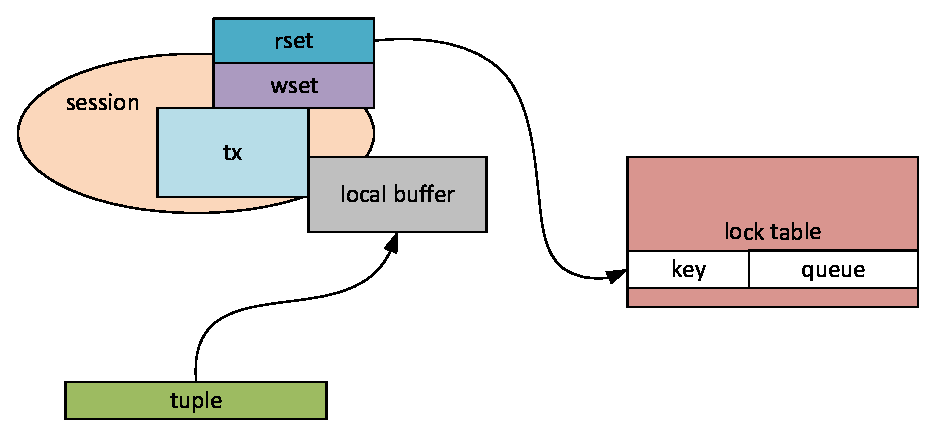
\includegraphics[width=\linewidth]{handout/img/7-rset.eps}
    \caption{读集合实现}\label{fig:7-rset}
\end{figure}

\subsubsection*{读集合}

读集合实现一般会利用锁表，读一行，会加读锁，锁进入全局锁表，每个事务自己还必须跟踪这个锁。如前所述，基于SI的方案，不会被阻塞，这个读锁也不会阻塞自己以及其它事务。这个锁不同于锁方案的锁，它的相容性矩阵不同，不会阻塞写锁。——此锁非彼锁。

在\figurename\ref{fig:7-rset}中，事务$tx$在会话中执行，它将一个tuple读到会话本地的局部缓冲，在锁表中加读锁，这个读锁的索引在事务本地以一个链表形式维持，指针指向全局锁表的表项。

在多版本模型下，读锁是加在版本上的，写锁也是加在版本上的，但是会影响上一个版本的读锁。

\subsection{SSI}

WSI方案中，只要读集合被修改，在提交时刻就无法通过rset的检查，会被取消。正如在锁方案中所了解到的，在调度中出现冲突并不可怕，冲突只是提示了事务两两之间的前后串行顺序，只要提交顺序与这个顺序一致，就不会出现问题。WSI的方案太过侵略性，损失了许多合法的调度。

SSI\cite{cahill2009serializable}与WSI相比，要精细一些，但它仍然没有完整检测环，仍然会出现误杀现象。

\begin{algorithm}[H]\label{alg:ssi}
    \caption{SSI Commit $\mathrm{commit}(T)$}
    \begin{algorithmic}[1]
        \State \textbf{atomically:}
        \State \quad \texttt{set } $T.\text{running} = \text{false}$
        \If{$T.\text{inConflict} \land T.\text{outConflict}$}
            \State \texttt{abort}$(T)$
            \State \Return UNSAFE\_ERROR
        \EndIf
        \Statex \Comment{existing SI code for $\mathrm{commit}(T)$, do not release SIREAD locks}
        \If{$T$ holds any SIREAD locks}
            \State suspend $T$, keeping SIREAD locks active
        \EndIf
        \If{$T$ was the oldest active transaction}
            \State clean up any suspended transactions older than active transactions
        \EndIf
    \end{algorithmic}
\end{algorithm}

SSI在每个事务引入两个bool变量：$T.\text{inConflict}$和$T.\text{outConflict}$，分别表示事务在冲突图上是否有入边和出边，暗示是否有环。每次事务开启，都会分配起始时戳，清掉这两个变量。

在事务提交时，SSI检查事务的$T.\text{inConflict}$和$T.\text{outConflict}$是否为真，同时为真则取消提交，意思是既有出边又有入边，说明事务在冲突图上可能有环，无法提交。这个入边出边主要是在读写操作时，根据rw冲突填写。在组提交策略下，一般是其它事务更新该事务的读集合，会产生一个出边标记，入边标记只会在短暂的提交阶段出现。

SSI的怪异之处在于第7行，事务已经提交，仍然需要维持该事务的读锁，直到与该事务的rset有交集的所有事务都提交或者取消。意思是要维持一个僵尸事务rset，用于判断是否有环。

SSI方案的出发点是利用\theoremname\ref{theorem:7-circle}，但在实际系统中，一般事务提交会释放所有锁，而rset是用读锁实现的。事务一旦提交，需要释放锁，销毁它的rset。这样一来就无从判断一个调度是否出现环，因为环上某个因果链缺失了，环被打断了。

\begin{algorithm}[H]\label{alg:ssi-write}
    \caption{SSI Write $\mathrm{write}(T, x, x\text{New})$}
    \begin{algorithmic}[1]
        \State \textbf{get lock}$(key = x,\ owner = T,\ mode = EXCLUSIVE)$
        \For{each conflicting SIREAD lock $(rl)$}
            \If{$rl.owner.running \lor \mathrm{commit}(rl.owner) > \mathrm{begin}(T)$}
                \If{$rl.owner \text{ is committed} \land rl.owner.inConflict$}
                    \State abort$(T)$
                    \State \Return UNSAFE\_ERROR
                \EndIf
                \State set $rl.owner.outConflict = \text{true}$
                \State set $T.inConflict = \text{true}$
            \EndIf
        \EndFor
        \Statex \Comment{existing SI code for $\mathrm{write}(T, x, x\text{New})$, do not get the EXCLUSIVE lock again}
    \end{algorithmic}
\end{algorithm}

SSI除了在提交时刻检查是否可能出现环，还会在wset上检查是否可能出现环。如\algorithmname\ref{alg:ssi-write}，当前事务有入边，而wset上有新版本，可能出现环。

\begin{example}
    用SSI方案处理\examplename\ref{ex:7-skew1}：
$$
m = r_1(x)r_2(y)w_1(y)c_1w_2(x)
$$
当事务$t_1$提交，只有一个入边，按照SSI提交协议\ref{alg:ssi}，$t_1$会被允许提交，同时标记$t_2$有一条出边。当$t_2$提交，写入$x$，发现$t_1$在读$x$，注意此时$t_1$已提交，因此标记为一条入边。这样，$t_2$的$\text{inConflict}$和$\text{outConflict}$都为true，回滚。
\end{example}

\begin{example}
    用SSI方案处理\examplename\ref{ex:7-skew2}：
$$
m = r_1(s)w_1(y)r_2(s)w_2(z)c_1
$$
在组提交策略下，$t_1$提交写入$y$，出现一条入边，同时标记$t_2$有一条出边。当$t_2$提交，准备写入$z$，此时$t_1$已提交，但有一个僵尸事务在维持rset，然后出现一条入边，因此$t_2$回滚。
\end{example}
\begin{example}
    用SSI方案处理\examplename\ref{ex:7-skew5}：
$$
m=r_1(x)w_2(x)c_2w_1(x)c_1
$$
按照组提交策略对原调度修改，$t_2$先提交，写入$x$新版本，事务标定入边，设定$t_1$有一条出边。当$t_1$提交，先尝试写入$x$，按照\algorithmname\ref{alg:ssi-write}，会检查$x$是否有新版本，如果有，写入新版本的事务已提交且有入边，则回滚。
\end{example}

\begin{example}\label{ex:ssi}
    SSI会导致误杀，这里构造一个用例。假设有一个公司有两张表，一张是当前的销售表，一张是按月的销售收入统计表。在下月的第1天统计上月的销售情况，更新销售收入统计表。
$$
m = r_1(x)r_2(y)w_2(x)c_2r_3(z)w_1(z)c_1
$$
在上述调度中，$t_1$对应于统计事务，$t_2$是一个更新销售表的事务，$t_3$是一个读取销售收入统计表的只读事务。$x$表示销售表的tuple，$y$表示销售收入统计表的tuple，$z$表示统计表的另一个tuple。

这个调度的冲突集是$conf(m)=\{(r_1(x),w_2(x)), (r_3(z),w_1(z)) \}$，对应的冲突图如下：

\begin{figure}[H]
    \centering
    \begin{tikzpicture}[node distance=4cm, auto, >=stealth]
        % 事务节点
        \node[draw, circle, minimum size=1.2cm] (t1) {$t_1$};
        \node[draw, circle, minimum size=1.2cm, right of=t1] (t2) {$t_2$};
        \node[draw, circle, minimum size=1.2cm, left of=t1] (t3) {$t_3$};

        % 冲突边
        \draw[->, thick] (t1) to node[above, align=center] {$r_1(x),w_2(x)$} (t2);
        \draw[->, thick] (t3) to node[above, align=center] {$r_3(z),w_1(z)$} (t1);
    \end{tikzpicture}
    \caption{SSI误杀案例}
    \label{fig:ssi-false-positive}
\end{figure}

冲突图中，没有出现环，可串行化。但按照SSI算法，$t_1$提交时，会出现入边和出边，判断为可能出现环，被放弃，出现误杀。

\end{example}

\begin{exercise}
    用SSI方案处理\examplename\ref{ex:7-skew3}。
\end{exercise}
\begin{exercise}
    用SSI方案处理\examplename\ref{ex:7-skew4}。
\end{exercise}

\subsubsection*{僵尸事务}

SSI\cite{cahill2009serializable}并没有详细描述僵尸事务如何维持，基本思路参考\figurename\ref{fig:7-zombie}，$t_x$事务的起始时戳和提交时戳用于区隔，系统范围内只要存在一个事务落在这个范围内，并且与$t_x$的rset有交集，则必须保留这个僵尸事务。

在\figurename\ref{fig:7-zombie}中，$t_3$事务无需考虑，$t_1, t_2$事务完结就可以删除僵尸事务。但是，实际系统中，只要$t_1$不提交，是无从了解是否与rset有交集的。因此，僵尸事务的清理条件为，Active Transaction Table, ATT表中的启动时戳大于$t_x$的提交时戳，就可以清理$t_x$的遗留信息了。

\begin{figure}[H]
    \centering
    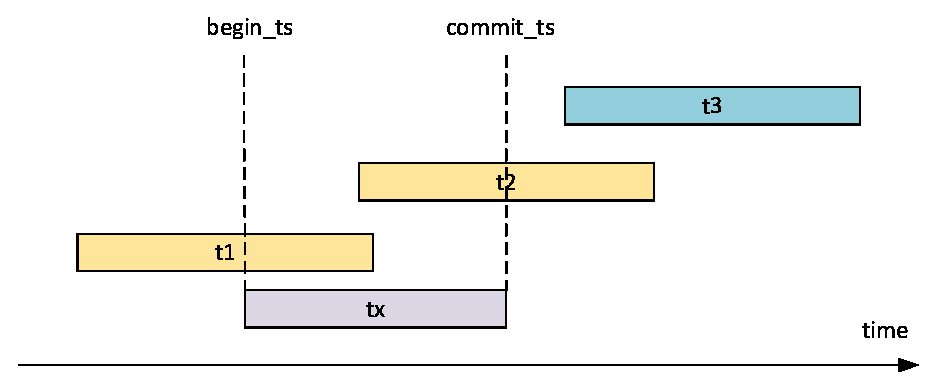
\includegraphics[width=0.8\linewidth]{handout/img/7-zombie.eps}
    \caption{僵尸事务实现}\label{fig:7-zombie}
\end{figure}

\subsection{CSI}

SSI方案通过保留僵尸事务来维持rset，用于判断是否出现环，付出的成本是维护僵尸事务，并且可能出现误杀。这里提出一种无环检测的SI可串行化方案，检测提交事务是否出现冲突环，称为CSI，unCircular SI。CSI的基本思路是，冲突并不可怕，冲突提示了事务提交的顺序，将这些提示收集为一个集合，当事务提交时，检查是否违反冲突提示即可。

\begin{figure}[H]
    \centering
    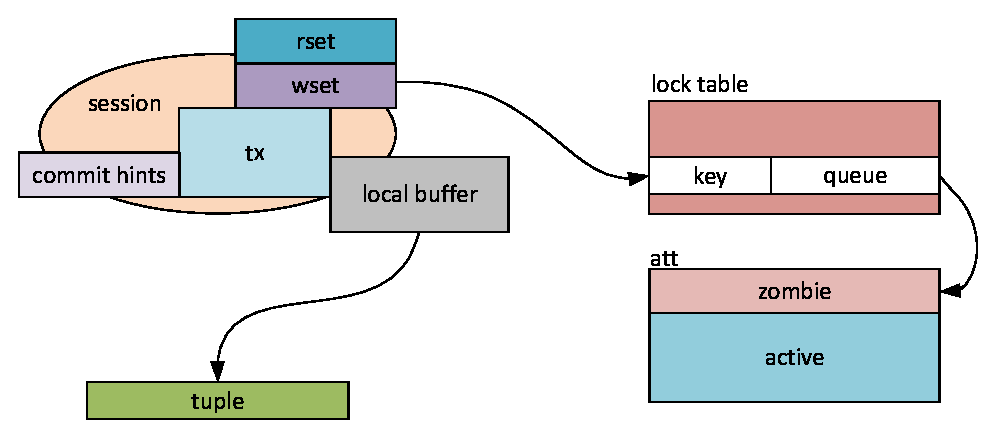
\includegraphics[width=\linewidth]{handout/img/7-csi.eps}
    \caption{CSI实现}\label{fig:7-csi}
\end{figure}

如\figurename\ref{fig:7-csi}所示，CSI在事务中增加了一个提交提示表。已提交事务在写入数据时，会产生rw冲突，这些冲突会被传递给各事务的提交提示表，该表记录了冲突图上该事务的所有出边。当该事务提交，检查wset，填写所有rset冲突事务的提交提示表，在填写时检查本地的提交提示表，如果匹配则出现环，取消写入，回滚。——此为方案一。

方案一，仍然不能避免所有环。将已提交事务之间的rw关系做剪枝，让事务指向未提交事务。——此为方案二，方案二更完整。

方案三，结合\figurename\ref{fig:7-zombie}，过滤掉所有提交时戳小于该事务的启动事务的已提交事务。

\begin{example}
    利用CSI处理\examplename\ref{ex:ssi}：
$$
m = r_1(x)r_2(y)w_2(x)c_2r_3(z)w_1(z)c_1
$$
$t_2$提交，在$t_1$的提交提示表中添加$commit\_ts(t_2)$，然后提交成功。$t_1$提交，由于更新的是$z$，在$t_3$的提交提示表中添加$commit\_ts(t_1)$。然后剪枝已提交事务的冲突图，在$t_3$的提交提示表中，添加$commit\_ts(t_2)$。
\end{example}

\section{对象的并发}

前述的单版本、多版本的并发都是基于行模型，更复杂的是对象模型。对象模型在行模型基础上，会组合成语义更复杂的上层操作，如\figurename\ref{fig:7-tree}。用户调用事务接口总是从上层开始的，这些操作最终被分解为行模型的叶子节点上的操作。考虑到各种操作可能会异步执行，\figurename\ref{fig:7-tree}的执行会以偏序森林的方式执行，对象的并发以这种偏序森林为模型展开讨论。

以一个web服务为例，一般会在服务端设置应用服务器，底层存储数据库。如果该web服务向外暴露事务接口，该接口的内部实现一般分层实现。以银行账户转账接口为例，应用服务器实现对单个账户的取款withdraw和存款deposit，取款与存款动作再分解为底层数据库行上的操作。两个转账事务$t_1, t_2$，$t_1$将钱从a账户转到b账户，$t_2$将钱从b账户转到c账户，\figurename\ref{fig:7-object}展示了这两个事务的并发执行过程。

\begin{figure}[H]
    \centering
    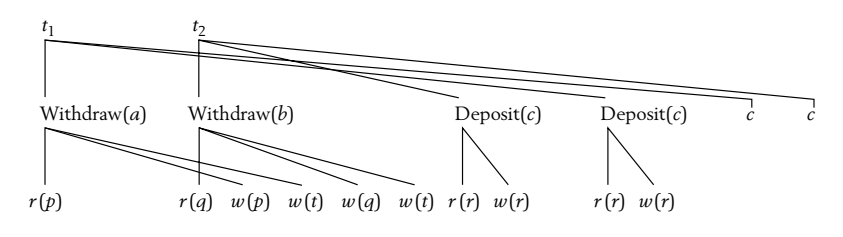
\includegraphics[width=\linewidth]{handout/img/7-object.png}
    \caption{对象并发执行}\label{fig:7-object}
\end{figure}

观察\figurename\ref{fig:7-object}，在根节点，两个事务顺序执行。但分解到取款与存储动作后，两个动作就开始并发执行。如果允许单个事务内部分层执行可以异步并发，例如存款取款并发由多个线程执行，可以想象，这种分层结构的操作构成了复杂的偏序森林。在形如\figurename\ref{fig:7-object}模型上讨论对象并发的正确性，就显得很复杂。

但实际上，对象并发性在学术届很少被讨论。对这个问题我们有几个判断：一个高层的事务接口被分解为行模型后，底层行模型的并发能保证多个事务并发的正确性。这个正确性有几个方面前提，前提一，要求单个事务并发后执行正确。一般会以一个线程对应一个用户会话，虽然理论上允许多线程并发实现高层事务，但实际系统中没这么复杂。前提二，高层事务能最终分解为行模型，这并不总是成立的，因为系统内部有一些维护程序，它们的动作也会被看成一些事务，这些维护程序并不是以行模型为叶子节点。

\section{谓词锁与锁表方案}

在前述的讲解中，我们都假设对行加锁，这简化了问题。但在实际应用中，SQL语句的WHERE子句会使用复杂的谓词限定查询范围，然后读取数据修改。如果谓词是单行，容易实现，麻烦的是范围锁如何处理。一种方案是将它们转换为行级锁，这个开销其实不小，因为需要在锁表中创建大量的行级锁。另一种方案是在采用Innodb的gap锁，对范围内所有行加锁，同时为防止幻读，对行与行间的间隙加锁。这两种方案都是基于btree，要对范围内的所有行加锁。

从上面的分析可以看到，将谓词转换为行或索引上的锁，并不是一种很好的方案。有几个方面的问题，首先要正确的将谓词转换为行上的操作；其次是行锁的粒度太小，锁表会非常大，导致锁表扫描成本过高；最后，还要防止幻读。所以，一般是直接将谓词处理为锁，称为谓词锁。

\begin{figure}[H]
    \centering
    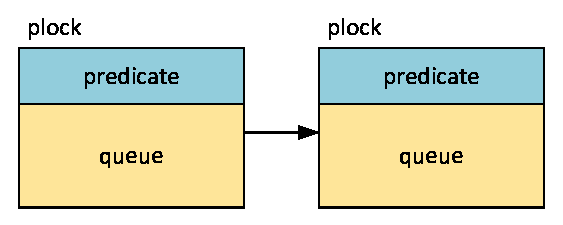
\includegraphics[width=0.6\linewidth]{handout/img/7-predicate.eps}
    \caption{谓词锁}\label{fig:7-predicate}
\end{figure}

谓词锁的实现如\figurename\ref{fig:7-predicate}所示，主要分为两部分，一部分是谓词，谓词表现为一个函数对象，范围一个bool值，当执行这个函数对象，返回true时，说明该谓词对当前行成立，对当前行加锁。另一部分是队列，用于存放等待的事务。

\figurename\ref{fig:7-predicate}中，谓词锁构成一个链表，要挨个尝试完队列中的所有谓词锁，分别确定哪些需要加锁。这个开销是比较大的，因为要遍历队列中的所有元素。

一个完整的、工程可用的锁表方案，并不容易，要容纳不同粒度的锁，如行级锁、范围谓词锁等。\figurename\ref{fig:7-predicate}将所有谓词堆砌在一起，性能不好。

mvcc的锁其实用得不多，SSI方案需要借助于锁表实现rset，在OLAP场景中，mvcc的锁表会非常大，导致锁表扫描成本过高。Neumann\cite{neumann2015fast}借助于precision lock\cite{jordan1981precision}方案，用谓词表达式来替代rset表示，而wset一般是点集，在多版本模型下，wset会自然体现为新版本。在提交验证阶段，用当前事务的wset的点去测试已提交事务的rset，同时检查rset上是否有新版本，如果有则用新版本测试提交事务的rset。

\begin{figure}[H]
    \centering
    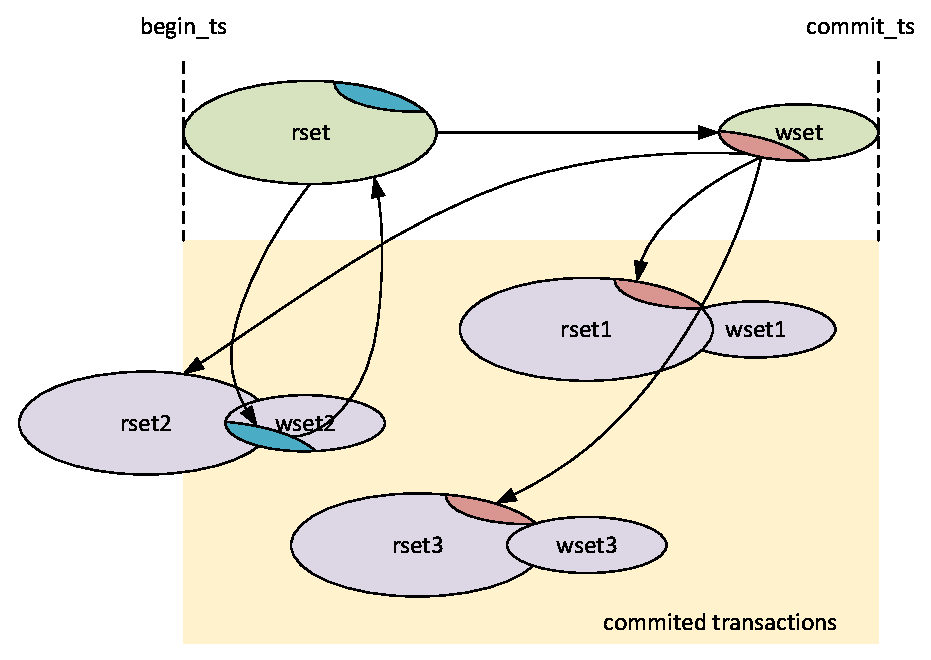
\includegraphics[width=0.8\linewidth]{handout/img/7-pt.eps}
    \caption{使用谓词锁替代rset}\label{fig:7-pt}
\end{figure}

如\figurename\ref{fig:7-pt}所示，在提交验证阶段，从两个方面验证rw冲突：1. 提交事务自己的rset用谓词表示，去rset上寻找被修改的行，找到后将这些新版本去匹配rset的谓词；2. 用当前wset上的点去测试过往已提交事务rset的谓词，找到冲突集。
 % 7
\chapter{Recovery}

事务主要包含两个大的功能：并发与恢复，上一章介绍了事务的并发控制，本章讨论事务的恢复。

\section{故障模型}

单机故障模型假设数据库系统运行在一个单机上，故障发生，系统崩溃，当系统重启，系统回滚恢复到崩溃前的状态，所有未完成事务被放弃。而在云计算中，要求提供7*24小时的服务，这就要求数据库系统必须要提供高可用性，即系统崩溃后，能够快速恢复到正常状态。

单机故障恢复主要依赖于日志WAL，在系统重启后，先分析日志，找到最近的checkpoint，然后从checkpoint后的日志开始回放，恢复状态。云计算的系统主要依赖于冗余提供高可用性，某个节点崩溃，其它可用节点能够快速接管，提供服务。云计算中的节点仍然高度依赖日志回放，副本节点通过全局日志回放接管服务。

单机故障模型和云计算故障模型的区别是明显的，前者依赖于持久化存储设备上的日志，后者还依赖于心跳+Paxos协议等来实现全局状态的一致。本章的内容主要讨论单机故障模型的恢复，云计算故障模型的恢复会在后续章节介绍。

\begin{exercise}
    单机故障模型下，认为日志总是是可靠的。实际系统中，日志也不一定总是可靠的，如何保证日志的可靠性？
\end{exercise}

\subsection{扩展行模型}

在单机故障中，系统恢复的是已提交的事务，未提交的事务被回滚。回滚要撤销该事务的所有修改，将数据库恢复到事务开始前的状态，它是一个逆操作。我们仍然从简单的模型开始讨论，先讨论行模型的回滚，然后再讨论对象模型的回滚。

行模型有两个操作，读和写，其中只有写操作会对行做修改，因此只有写操作需要实现逆操作。行模型是一个抽象模型，写的逆操作是恢复之前的行。考虑下面的一个调度：
$$
s = r_1(x)w_1(x)r_2(x)a_1w_2(x)c_2
$$
这个调度中，$t_1$事务回滚，要撤销之前的修改，将$x$恢复到$w_1(x)$之前的状态，$a_1$会执行逆操作$w_1^{-1}(x)$，其实际执行的调度是：
$$
s' = r_1(x)w_1(x)r_2(x)w_1^{-1}c_1(x)w_2(x)c_2
$$
在本章的讨论中，形式化的调度在上一章并发控制的基础上，增加了提交和取消两个动作，取消或者回滚可以扩展为写操作的逆操作，然后归结于正常提交。

\subsection{行模型的可恢复性}

在调度中引入提交和取消动作，扩展了行模型。要判读一个扩展行模型的并发是否正确，仍然要看它是否冲突等价于一个串行化执行的调度。

\begin{example}\label{ex:8-recover}
考虑如下调度：
$$
s = r_1(x)w_1(x)r_2(x)a_1c_2
$$
这个例子中，$t_2$脏读了$x$。$s$的冲突集是$conf(s)=\{ (w_1(x),r_2(x))\}$，它的扩展调度是：
$$
s' = r_1(x)w_1(x)r_2(x)w_1^{-1}(x)c_1c_2
$$
无需考虑逆操作的冲突，$s'$的冲突集是$conf(s')=\{ (w_1(x),r_2(x))\}$，与$conf(s)$相同。但$t_1$的写操作$w_1(x)$已经被取消，这个调度有问题。
\end{example}

在处理扩展行模型时，取消操作$a$可以将整个事务的所有操作全部删除，删除后的等价冲突集不变。

\begin{example}\label{ex:8-recover2}
    考虑如下调度：
$$
s=r_1(x)w_1(x)r_2(x)w_2(x)a_2a_1
$$
它等价于如下的调度：
\begin{align*}
s' &= r_1(x)w_1(x)r_2(x)w_2(x)w_2^{-1}(x)c_2a_1 \\
   &= r_1(x)w_1(x)r_2(x)c_2a_1 \\
   &= r_1(x)w_1(x)c_2a_1 \\
   &= r_1(x)w_1(x)c_2w_1^{-1}(x)c_1 \\
   &= r_1(x)c_2c_1 \\
   &= c_2c_1
\end{align*}
\end{example}

仔细观察两个例子，\examplename\ref{ex:8-recover2}能正常恢复，而\examplename\ref{ex:8-recover}是有问题的。本章引入扩展行模型的的目的是为了讨论事务的恢复，\examplename\ref{ex:8-recover}是不可恢复的。这里不形式化定义可恢复性，可以参考\cite{Weikum2001Transactional}。

一个基本常识：如果扩展行模型的所有事务正常提交，或者说可串行化，那么以逆序方式取消事务，得到的调度是可恢复的。

\examplename\ref{ex:8-recover}的脏读例子，为了使得调度正确，需要使得$t_2$被回滚，这称为级联回滚。一般来说，级联回滚会使得系统的恢复时间增加，因此在设计数据库系统时，要尽量避免级联回滚。

\subsection{对象模型}

在上一章讨论事务并发时，我们引入了对象模型：我们假设，高层事务接口被分解为几个层次，最后一层是行模型。对象模型调度的正确性依赖于底层行模型的正确性，对象模型的可恢复性类似，我们寄望于底层行模型上能够实现可恢复性，那么对象模型的调度也是可恢复的。

在高层实现逆操作，开销非常大，设计难度很高，对象模型可恢复性由底层行模型实现是非常美好的。但是，这一原则并不总是有效，因为系统内总有些高层事务接口无法映射为行模型，例如对数据库文件页面的操作，操作的对象是页面而非抽象的行，要处理页面分裂合并等问题。

\section{wal}

上一节我们简单讨论了事务恢复在行模型上的可恢复性，技术上，在单机模型上实现逆操作需要日志的支持。因为取消动作并不只在并发才有，在系统恢复也会用到。基于日志的恢复方案主要源自ARIES\cite{mohan1992aries}，ARIES规范了恢复流程，解耦了并发与恢复，讨论了checkpoint的实现等。

数据库为了恢复，任何对数据库内部对象的修改，都要先记录日志，这称为write ahead logging（WAL）。WAL的实现一般要求文件系统支持journaling，并且由于日志是追加写入，日志条目的增加虽然变长，但是原子的。底层文件系统journalling机制的要求其实不低，从文件系统的发展来看，这个机制的完整实现都是很后来的事情了。

随着SSD器件的普及，wal的实现变得要简单一些\cite{GitHubgo38:online}，因为SSD内部有一套虚拟块号映射机制，追加写入要先分配一块新的地址，擦除原物理地址。

\subsection{物理日志与逻辑日志}

WAL记录的信息用于恢复系统，数据库系统是分层次的，底层是存储系统，上层是执行引擎、事务引擎等。日志需要记录哪些信息？从目前众多数据库的选择来看，不约而同选择底层存储系统的变化作为日志信息。其中的道理可以类比前述的对象模型，高层对象的操作最终会分解为底层存储系统上的操作。

一般而言，物理日志记录的是底层存储系统的变化，逻辑日志记录的是高层事务接口的变化。数据库日志一般以物理日志为主，但并不排除跨层记录的情形，例如2PC协议，prepare阶段需要记录状态。

\begin{exercise}
    在分布式系统中，存储系统分为share nothing或者share everything两种设计。为了提供7*24不间断服务，一般会采用Paxos/Raft协议提供冗余，这些协议是否要记录日志？
\end{exercise}

在ARIES的设计中，基本上是以buffer管理为界线，如\figurename\ref{fig:1-arch}，其上为高层，其下是存储系统。可以说，ARIES是面向存储系统的日志机制。

这里有必要再回顾一下，前述的事务并发控制基于行模型，行模型是一个高层的逻辑模型。而日志系统是针对底层存储系统设计，两者之间有明显的设计差异。在后面的内容中，要注意观察高层的恢复需求是如何体现在底层日志系统的设计上的。

\subsection{日志的结构}

日志是有结构的，正如第\ref{chap:layout}章的记录。按照ARIES的方案\cite{mohan1992aries}，一个日志条目包含如下字段，这些字段设计的必要性在后介绍。

\begin{itemize}
    \item LSN：日志条目编号，全局唯一，递增。有些系统中的LSN是日志文件中的偏移量，在日志条目中并没有这个字段。oracle数据库中，SCN是一个逻辑时戳。
    \item checksum：校验和，用于检查日志是否损坏。
    \item length：日志条目长度。
    \item type：日志类型，update、compensation、checkpoint、prepare等。
    \item tid+prevLSN：事务号以及该事务的前一个日志条目编号，用于构建事务的日志链。
    \item pageid：页面编号。
    \item undoNxtLSN：补偿日志的指针。
    \item data：日志载荷。
\end{itemize}

\begin{exercise}
    Oracle的SCN为什么设计为一个逻辑时戳？
\end{exercise}

从设计的弹性来看，一般用type来标记特定的函数对象，data标记函数对象的调用参数，如\figurename\ref{fig:8-wal}所示，其中payload部分的设计模仿第\ref{chap:layout}章的记录。

\begin{figure}[H]
    \centering
    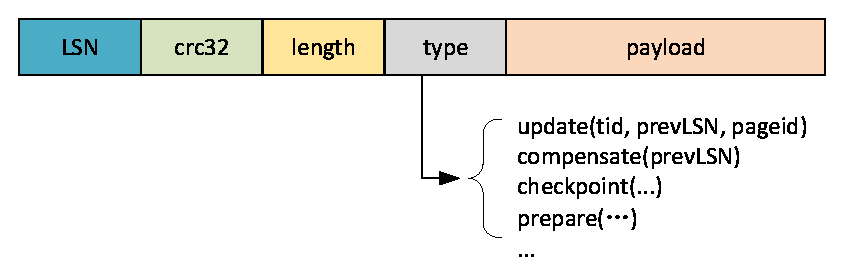
\includegraphics[width=0.8\linewidth]{handout/img/8-wal.eps}
    \caption{WAL日志格式}\label{fig:8-wal}
\end{figure}

日志文件用追加方式写入，多数文件系统会提供原子追加操作。日志条目之间，不用添加特殊分隔符，因为日志条目的扫描从checkpoint开始向后扫，每个条目包含长度信息。如果出现校验损坏，其后的日志条目也是不可信的，要放弃。

\begin{exercise}
    如果扫描日志条目，遇到校验损坏的条目，为什么要放弃后续日志的扫描？
\end{exercise}
\begin{exercise}
    模仿第\ref{chap:layout}章的记录，补充\figurename\ref{fig:8-wal}的payload设计。
\end{exercise}

\section{基本功能}

本节开始讨论日志需要支持的功能及其实现方案，数据库日志的功能设计是具有弹性的，并不是固定的。本讲义从最简单的需求开始，逐步丰富日志的功能，堆砌出一个完整的日志框架。

\subsection{update}

考虑在行模型中，写一行数据如何在底层存储系统上实现。如\figurename\ref{fig:8-update}所示，一个在session运行的事务，要将本地缓冲的行写入一页。先在锁表中加锁，然后对页面上闩，在修改页面之前，先记录日志。

\begin{figure}[H]
    \centering
    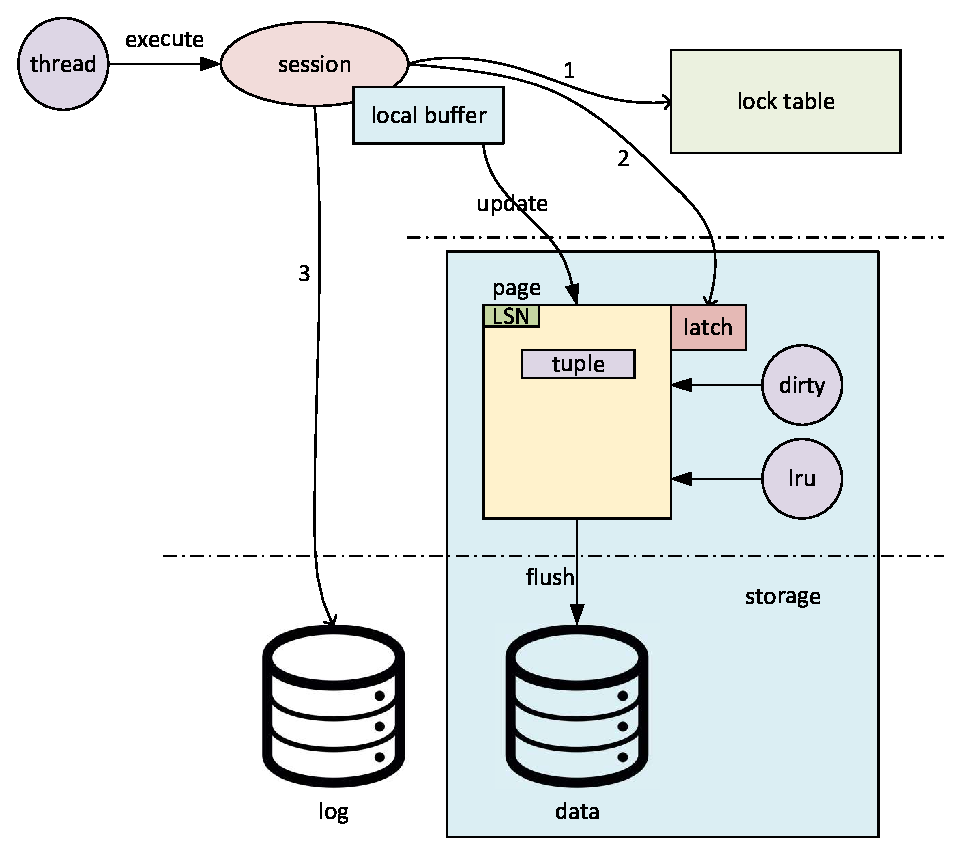
\includegraphics[width=0.8\linewidth]{handout/img/8-update.eps}
    \caption{写一行过程}\label{fig:8-update}
\end{figure}

\begin{exercise}
    \figurename\ref{fig:8-update}所示为锁方案，假设采用第\ref{chap:concurrent}章两种rset维持方案，该如何处理？
\end{exercise}

在锁方案中，对行更新可能会导致死锁，需要一个死锁检测与解锁机制。在mvcc中，由于读锁不会阻塞事务推进，所以不需要死锁检测。\figurename\ref{fig:8-update}对页面加锁也可能会导致闩的死锁，如果采用组提交策略，在提交阶段写入，以first-commit-wins策略可以避免这一问题。——可以看到，mvcc比锁方案先进太多，规避了很多难题。

\figurename\ref{fig:8-update}中，存储引擎包含了缓冲管理、底层存储管理、文件管理等功能，日志是针对这一层设计。页面由缓冲层管理，一般内置脏链、lru链，当缓冲层的页面不敷使用，会下刷dirty页面或者释放干净页面。

另一个值得注意的是，\figurename\ref{fig:8-update}解耦了事务处理与数据刷新。事务对数据的更新只到缓冲层的页面，脏页面的刷新由缓冲管理层负责。

\begin{exercise}
    假设系统不支持脏读，\figurename\ref{fig:8-update}中的latch会导致死锁发生吗？
\end{exercise}

\subsubsection*{undo+redo}

考虑日志的设计，对一个对象的修改，需要记录两个信息：UNDO+REDO。前者用于回滚，后者用于恢复，两类信息是必需的，缺一不可。但在实现中，可以将UNDO和REDO拆开为两条日志，先记录UNDO，然后记录REDO。

\begin{figure}[H]
    \centering
    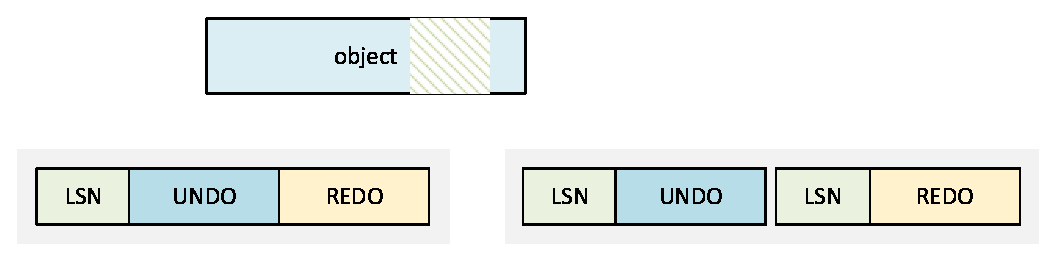
\includegraphics[width=0.8\linewidth]{handout/img/8-modify.eps}
    \caption{undo+redo}\label{fig:8-modify}
\end{figure}

如\figurename\ref{fig:8-modify}所示，对于一个对象的update操作，有两种方案，一种是在一条日志中记录所有UNDO+REDO，另一种是先记录UNDO，然后记录REDO。

\begin{exercise}
    \figurename\ref{fig:8-modify}中，为什么一定要先记录UNDO？可不可以先记录REDO？
\end{exercise}

采用read-only+undo-only的日志方案，需要在type字段补充一些信息。因为在系统恢复阶段，日志会被重放，所以仍然要在undo-only日志中类型中标记update，意思是这个undo日志在更新中不需要执行。

\subsubsection*{页面结构}

日志是针对存储系统设计的，关系型数据的存储都是按页组织的，undo+redo日志中一定会包含pageid，在系统恢复中，这些信息足够了。但是，另一个场景是，一个事务修改了页面，但后来又被取消，页面需要回滚。

要提供页面回滚功能，可以扫描日志，找到对该页面的undo条目，撤销该页面的修改。这个过程太漫长了，为了方便页面的回滚，在页面上设计了一个LSN字段，指向日志条目。

\begin{figure}[H]
    \centering
    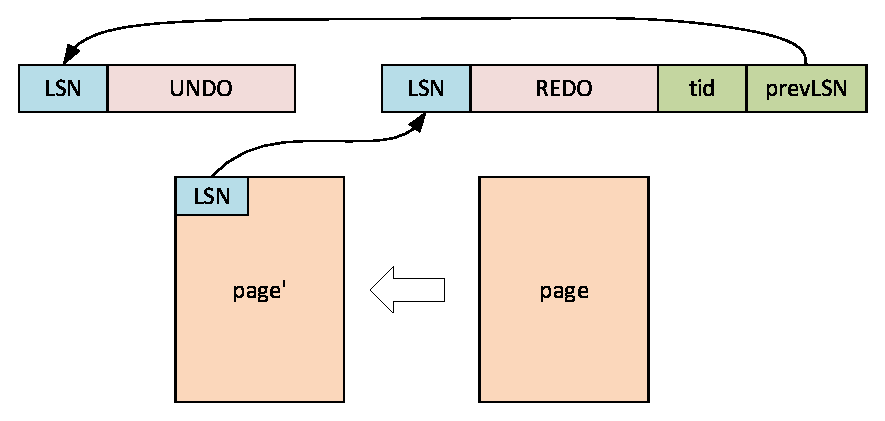
\includegraphics[width=0.7\linewidth]{handout/img/8-prev.eps}
    \caption{事务日志前驱指针}\label{fig:8-prev}
\end{figure}

在\figurename\ref{fig:8-prev}中，为快速定位修改页面的日志条目，在页面结构上增加一个字段LSN。LSN指向修改该页面的REDO日志，REDO日志带上prevLSN指针，指向前一个日志条目，顺着这个逆向链表，可以快速定位该页面的undo日志。

\begin{exercise}
    \figurename\ref{fig:8-prev}中，LSN为什不指向的UNDO日志？
\end{exercise}

从页面LSN字段的设计，可以获得一个技能：要快速回滚某个对象，只需在对象上带上LSN字段即可。\figurename\ref{fig:8-prev}中，prevLSN并不是指向UNDO日志，它实际上维护了一个事务的修改历史链表，这是为了方便事务的管理，日志源一般都是事务。可以看到日志的设计是非常有弹性的，并没有绑死在存储系统上。

\subsection{rollback}

回滚要求撤销事务之前的修改，系统恢复时，需要撤销未完成事务的修改。此外，事务由于并发原因，可能会被取消重启，也需要回滚功能。SQL标准要求实现savepoint，以提供更细粒度的回滚能力，不必撤销整个事务的所有修改，只撤销部分。还有些情况下，允许子事务嵌套，当子事务被取消，也需部分回滚。

回滚的实现，要借助于前述update的undo日志，ARIES中将回滚动作称为补偿日志，compensation log record，CLR。前述的undo日志只是提供了回滚的操作，CLR是执行这个操作的标志。任何对数据库状态的修改，都需记录在案，包括CLR日志。

举例而言，一个系统崩溃，重启后恢复，undo了一些修改，此时再次崩溃，如果不记录CLR日志，可能会undo多次，系统将处于一种未知的不安全状态。

\subsubsection*{ATT}

活跃事务表active transactions table, ATT表记录所有系统当前活跃记录，即未提交事务表。ATT表是事务模块管理的一个表，在系统崩溃自举后，ATT表需要参与系统修复。

系统重启，先找到最近的checkpoint，然后开始扫描日志，重放日志。当遇到一个事务开启，将该事务加入ATT表，该事务提交或者取消，从ATT表剔除这个事务。对于修复来说，关心的是，所有日志重放完毕，ATT表还剩下哪些事务，这些事务将被取消。

ATT表记录了事务的状态，每个事务包含的状态如下，其中undoNxtLSN的含义在后面解释。

\begin{itemize}
    \item tid：事务编号，单增，全局唯一。
    \item status：事务状态，活跃、提交、取消。
    \item begin\_ts：事务开始时间戳。
    \item end\_ts：事务结束时间戳。
    \item lastLSN：事务最后一个日志条目的LSN。
    \item undoNxtLSN：事务下一个undo日志条目的LSN。
\end{itemize}

\subsubsection*{补偿过程}

回滚过程如\figurename\ref{fig:8-clr}所示，日志记录了对page对象的操作过程，$\{1, 2, 3, 3', 2', 4\}$，其中$\{3', 2'\}$是CLR日志，将page状态回滚到$1$之后的状态，然后应用日志$4$更新page。

\begin{figure}[H]
    \centering
    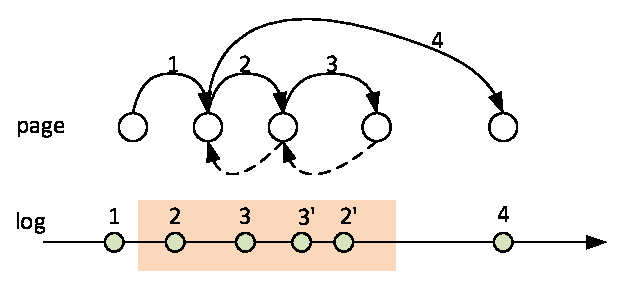
\includegraphics[width=0.6\linewidth]{handout/img/8-clr.eps}
    \caption{补偿日志}\label{fig:8-clr}
\end{figure}

CLR日志记录了对page对象的逆操作，它要指向前面的undo日志，以便应用该日志。同时undoNxtLSN指向CLR日志回退到的redo日志，这样系统重启后，可以直接跳过其间的日志条目，应用该CLR的下一条日志。如\figurename\ref{fig:8-clr}所示，$\{2, 3, 3', 2' \}$被跳过，$2'$下一条日志是$4$。

部分回滚牵涉到一个隐秘的问题，是否释放回滚部分获得的锁？如\figurename\ref{fig:8-clr}所示，$2, 3$获取行锁，$\{3', 2' \}$部分回滚后，这些锁需要释放。——这看起来违反了2PL协议，但是在道理上是讲得通的。如果不释放这些锁，由于扩大了事务资源的获取范围，死锁的风险会加大。

\subsection{swap}

如前所述，ARIES方案解耦了事务执行与缓冲管理，事务执行时，只需要关注对缓冲模块的操作，而缓冲模块的操作，只需要关注对磁盘的操作。在缓冲的设计中，一般不会允许缓冲容量无限制的增长，通常简单的做法是直接限制缓冲大小。

当缓冲不敷使用，就必须为新的页面请求腾挪出足够的空间。swap的策略很多，一般是直接使用lru，将lru队尾的页面换出，直到有足够的空间。lru并不管页面是否脏，干净页面直接释放，脏页面下刷。这些脏页面下刷，也需记录日志，可以将缓冲管理器看成一个内部事务，加入ATT表。

这些页面下刷的动作，仍然先写UNDO日志，REDO日志就不再需要了。注意到此时脏页面可能有未提交事务写入，所以数据库表并非只保存已提交事务的修改。数据库系统的状态并非只包含硬盘上的状态，而是硬盘+日志修正后的状态。

\begin{exercise}
    脏页面刷新，为什么不需要写REDO日志？
\end{exercise}

\figurename\ref{fig:8-swap}展示了脏页下刷，图中tid表示一个事务，buffer manager看成一个事务。所有日志条目看成日志流，这些日志条目抽象为堆。堆中的日志条目根据不同维度串联成链表，如按照事务，prevLSN串起了所有该事务的日志条目。另一个维度是页面，swap到磁盘上的页面，先UNDO一把，记录磁盘上之前的页面，当前LSN指向的日志包含一个指针指向上一个对该页面修改的日志。

\begin{figure}[H]
    \centering
    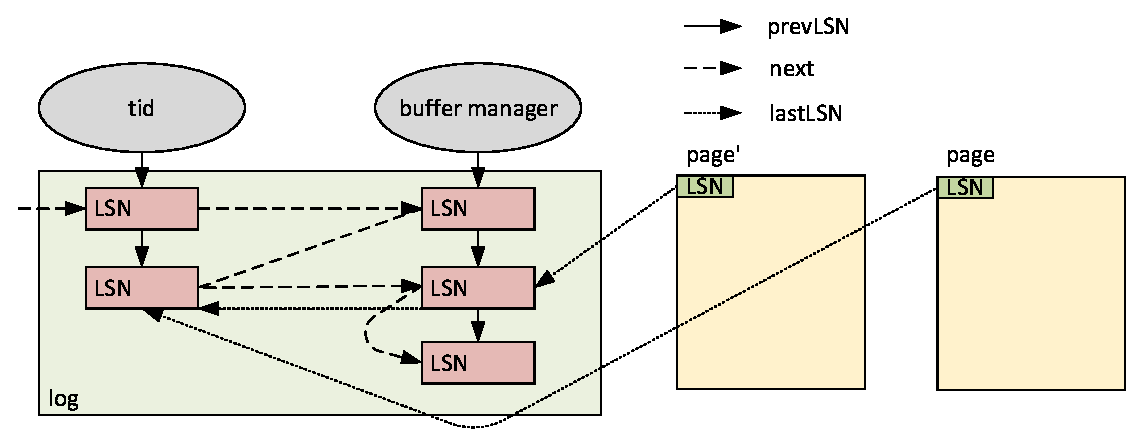
\includegraphics[width=\linewidth]{handout/img/8-swap.eps}
    \caption{脏页下刷}\label{fig:8-swap}
\end{figure}

日志格式是灵活的，在堆模型下，可以按照需要调整日志格式，如\figurename\ref{fig:8-swap}所示，日志中包含了对页面的修改，以及对页面的逆操作。

\section{Checkpoint}

检查点是需要的，日志文件长度不能无限增加，并且基于性能的考虑，系统自举后，要避免扫描日志开销过大。检查点是日志流中一类特殊的标记点，从它开始，系统可以重建。它是一个基线$b$，从它开始，每个日志条目代表一个对系统的修改$\Delta$，$b+\Delta_1+\Delta_2+...$最终重构系统状态。

\begin{figure}[H]
    \centering
    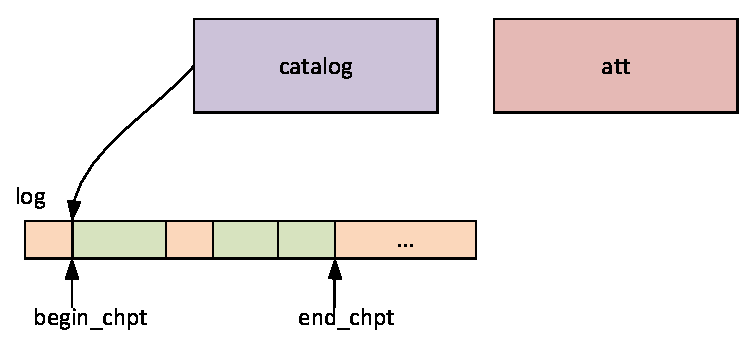
\includegraphics[width=0.6\linewidth]{handout/img/8-checkpoint.eps}
    \caption{fuzzy checkpoint}\label{fig:8-checkpoint}
\end{figure}

\subsection{fuzzy checkpoint}

早期的checkpoint构建要求系统松弛，即停止对外服务，找一个服务相对较少的时段，构建checkpoint，这称为sharp checkpoint。后来，发展出fuzzy checkpoint，以异步不停机方式构建checkpoint。

fuzzy checkpoint的实现方案如\figurename\ref{fig:8-checkpoint}所示，checkpoint被处理为一个内部事务。它启动后加入ATT表，构建过程中不断记录日志，构建完毕后，将catalog中的checkpoint位置指向begin\_ckpt的LSN。

checkpoint构建过程中，其它事务仍然执行，因此在日志流中，begin\_ckpt到end\_chpt之间可能会夹杂其它事务的日志。系统重启后，这些夹杂其间的日志会被识别出来，有些日志不会被redo，因为checkpoint在这些日志之后做总结。

接下去要考虑checkpoint需要做哪些基线。如\figurename\ref{fig:8-baseline}，首先是缓冲模块的脏页，这些页面要被写入磁盘，作为基线。其次是ATT表，它记录了系统当前活跃事务，这些事务要被写入磁盘。然后是catalog，对元数据的修改也需要记录在案，这些修改要被写入磁盘。

脏页面的处理除了交换到数据文件中，还需要转移一部分being\_chpt之前的UNDO日志到checkpoint上。脏页面的修改可能由ATT表上的活动事务做出，这些事务有被清退的可能，因此它们的修改UNDO日志要被转移到checkpoint上。

\begin{figure}[H]
    \centering
    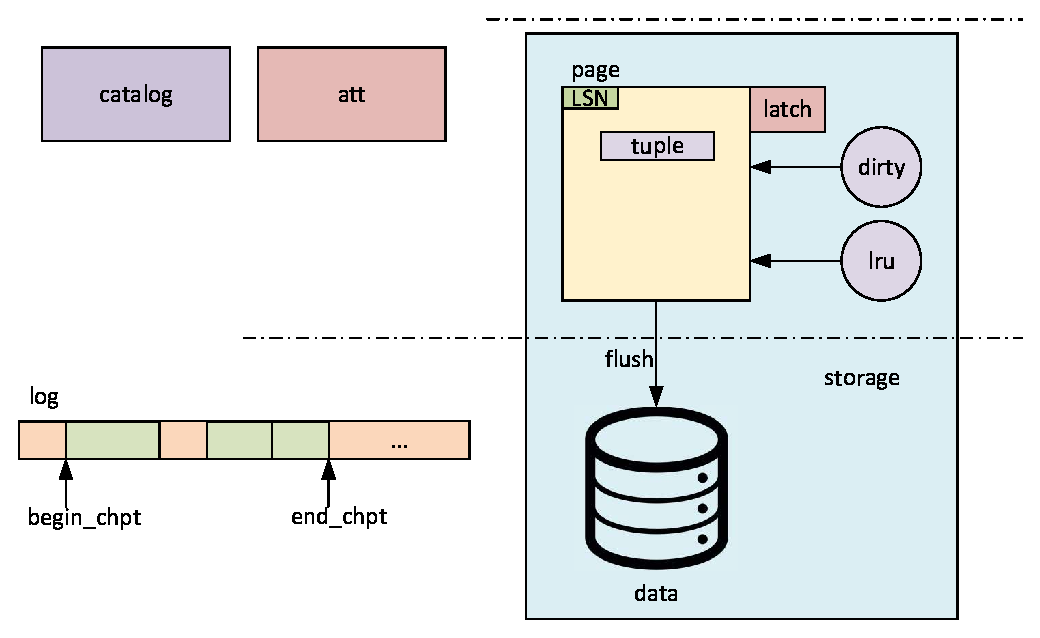
\includegraphics[width=0.8\linewidth]{handout/img/8-baseline.eps}
    \caption{checkpoint基线构建}\label{fig:8-baseline}
\end{figure}

打checkpoint需要将所有脏页落盘，这与缓冲管理层的flush功能不同，后者只是为了腾挪出足够的空间。checkpoint一般会周期性执行，也可以根据需要手动执行。

\begin{exercise}
    下刷了脏页，干净的页面怎么办？
\end{exercise}
\begin{exercise}
    checkpoint构建过程中，夹杂了部分其它事务修改记录，如何处理？如何识别哪些日志是需要在重启后redo？
\end{exercise}
\begin{exercise}
    前述的日志结构中，只有一个checkpoint类型，而checkpoint要执行的动作很多，这够吗？
\end{exercise}
\begin{exercise}
    打checkpoint，需要加锁吗？加latch的话，是否会影响其它事务的执行？
\end{exercise}

\section{系统重启}

系统重启过程，ARIES\cite{mohan1992aries}规范为三轮：

\begin{itemize}
    \item 第1轮，分析。要找到最近的checkpoint，以它为基线开始重放，一般会在catalog中记录。有些系统会打开日志，不断向前扫描，直到最近的checkpoint。在分析轮，要拉起事务模块和缓冲模块，准备好ATT表和空闲页面队列。
    \item 第2轮，重做。从checkpoint开始，顺序重放日志。新的事务开始，将它加到ATT表，然后执行它的REDO动作和补偿动作。写入页面操作，要buffer manager会先读取页面，读取完毕后，会检查该页面的LSN是否小于当前LSN。如果大于当前LSN，是因为这个页面被缓冲管理交换过，参考\figurename\ref{fig:8-swap}，按照链表找到小于当前页面的UNDO加载。当事务提交或者取消，从ATT表中驱逐这个事务。
    \item 第3轮，清扫。当所有日志重放完毕，ATT表内所剩的事务为未完成事务，处理为取消。应用这些事务的UNDO操作，将页面回退到前一个LSN，回滚前要记录补偿日志。
\end{itemize}

\begin{exercise}
    catalog非常重要，如何确保它的安全？
\end{exercise}

 % 8
% \input{distributed.tex}

% 参考文献
\printbibliography[heading=bibintoc]

% 附录
\appendix
% \chapter{术语表}

\end{document}